\documentclass[a4paper,10pt]{article}
%\documentclass[a4paper,10pt]{scrartcl}
\setcounter{secnumdepth}{0} %разделы без нумерации 
\setcounter{tocdepth}{2} % не показывать под-подразделы в оглавлении

\usepackage[utf8]{inputenc}
\usepackage[T1,T2A]{fontenc}
\usepackage[utf8]{inputenc}
\usepackage[english,russian]{babel}
\usepackage{xcolor} %для цветных блоков с текстом
\usepackage{mdframed} %для блоков с текстом
\usepackage{geometry} % Меняем поля страницы
\geometry{left=2cm}% левое поле
\geometry{right=1.5cm}% правое поле
\geometry{top=1cm}% верхнее поле
\geometry{bottom=2cm}% нижнее поле
\usepackage{graphicx} %вставлять картинки
\usepackage{array}
\usepackage{tabu}
\usepackage{keystroke}
\usepackage{menukeys}
\usepackage[normalem]{ulem} %для перечёркиваний
\usepackage{fixltx2e} %нижний индекс
\usepackage{marvosym}
\usepackage{enumitem} %иерархические списки
\usepackage{sectsty} % размер заголовков
\usepackage{longtable} %многостраничные таблицы
\usepackage{lipsum} %частные отступы для абзацев

\graphicspath{ {/home/mint/trans/freeoffice2016/tm_pics/} } %путь до картинок

\title{TextMaker\\ Руководство пользователя}
\author{}
\date{}

\pdfinfo{%
  /Title    ()
  /Author   ()
  /Creator  ()
  /Producer ()
  /Subject  ()
  /Keywords ()
}

\sectionfont{\fontsize{27}{24}\selectfont}
\subsectionfont{\fontsize{14}{18}\selectfont}
\subsubsectionfont{\fontsize{12}{12}\selectfont}
%\paragraphfont{\fontsize{11}{9}\selectfont}

\newenvironment{myindentpar}[1]%частные отступы для абзацев
 {\begin{list}{}%
         {\setlength{\leftmargin}{#1}}%
         \item[]%
 }
 {\end{list}}

\makeatletter
\renewcommand\paragraph{%
   \@startsection{paragraph}{4}{0mm}%
      {-\baselineskip}%
      {.5\baselineskip}%
      {\normalfont\normalsize\bfseries}}
\makeatother

\begin{document}
\maketitle
\tableofcontents
\section{Добро пожаловать!}

Добро пожаловать в TextMaker! Вы приобрели текстовый процессор, сочетающий в себе удобство использования с богатым функционалом по приемлемой цене. TextMaker предоставляет возможность пользователям выполнить задачи по написанию и обработке текстов быстро и с комфортом. 
\begin{mdframed}[backgroundcolor=pink!50]
\textbf{Внимание:} в SoftMaker FreeOffice (бесплатной версии SoftMaker Office) некоторые возможности отсутствуют. Отсутствующий функционал выделен розовым блоком, аналогичным тому, в который помещён данный текст.
\end{mdframed}
\subsubsection{Некоторые возможности TextMaker}
\begin{itemize}
\item Доступен для операционных систем Windows, Linux и Android
\item Удобные для работы шаблоны документов: готовые формы для писем, бланки факсов и т.п., позволяющие создавать документы в кратчайшие сроки
\item Расширенные возможности форматирования параграфов, включая автоматическую нумерацию, маркёры, обрамление, заливка и формы для заполнения
\item Стили параграфов и символов, позволяющие применять часто используемое форматирование к тексту нажатием одной кнопки
\item Возможности компьютерной вёрстки, такие, как главная страница, буквица, малые прописные, автоматический контроль абзацев, настраиваемый кернинг и шаг метки
\item Поддержка многочисленных графических форматов файлов, расширенные возможности рисования, модуль TextArt для затейливых текстовых эффектов
\item Разнообразные табличные функции, включая арифметические
\item Менеджер файлов и документов с поисковым функционалом
\item Создание оглавлений и алфавитных указателей, сносок и примечаний, показ контура
\itemПроверка орфографии, переносы и словари синонимов (не включённые в SoftMaker FreeOffice)
\itemВстроенная адресная книга (база данных)
\item… и многое другое!
\end{itemize}
Разработка TextMaker постоянно прогрессирует, и мы приветствуем отзывы и предложения от наших пользователей. Если в процессе работы вам понадобился функционал, отсутствующий на данный момент, или же у вас родились другие предложения --- напишите нам, мы хотим, чтобы TextMaker отвечал пожеланиям наших пользователей!
\subsubsection{Дополнительные возможности SoftMaker Office Professional}
Доступно только для ОС Windows и Linux:\\
Ещё более мощный \textbf{SoftMaker Office Professional} включает в себя расширенную версию TextMaker со следующими дополнительными возможностями:
\begin{itemize}
 \item Встроенные словари Berlitz для переводов --- дающие возможность перевода между пятью языками (Английский, Французский, Немецкий, Итальянский и Испанский) нажатием одной кнопки
\end{itemize}
\textbf{Версии для Android}\\
TextMaker также доступен для устройств на базе Android, в двух разных версиях:
\begin{itemize}
 \item TextMaker HD для Android\\
Эта версия содержит практически  все возможности версии для Windows и разработана для использования на планшетах
\item TextMaker Mobile для Android\\
Эта версия содержит только некоторые возможности версии для Windows и предназначена для использования на смартфонах.
\end{itemize}
Все инструкции данного руководства относятся к версии HD. (Для версии Mobile существует отдельное руководство.)
\subsection{Техническая поддержка}
Если у вас появились вопросы, наша команда технической поддержки будет рада помочь. Наши контакты:

\textbf{Вебсайт}

На нашем сайте можно найти программные обновления, полезные советы, ссылки для бесплатных загрузок и многое другое. Заходите на www.softmaker.com

\textbf{Форумы поддержки}

Обменивайтесь информацией с нашей командой техподдержки и с другими пользователями, на наших форумах поддержки по адресу forum.softmaker.com

\textbf{Почта}

Письма, касающиеся технической поддержки, шлите по адресу: support@softmaker.com

\subsection{Об этом руководстве}
TextMaker --- это программа с богатым функционалом, поэтому обилие возможностей может на первых порах показаться устрашающим. Не беспокойтесь, необязательно сразу знать все команды. В начале работы достаточно только тех, которые будут нужны непосредственно, а позже можно обратиться к соответствующим страницам Руководства.

В Руководстве по работе с TextMaker информация распределена следующим образом:
\begin{itemize}
 \item В главе «Установка и запуск программы» (стр.19) содержатся сведения об установке TextMaker.  Вы также узнаете, как запускать программу.
 \item В главе «Окно приложения» (стр.23) описываются отдельные компоненты главного окна TextMaker. Идеально для новичков!
 \item Глава «Базовые операции» (стр.29) знакомит с самыми главными командами TextMaker. То, что нужно новичкам!
 \item Глава «TextMaker в примерах» (стр.39) — это небольшой учебник по  теме редактирования текстов, который на практических примерах знакомит пользователя с операциями TextMaker.
 \item Глава «Работа с выделениями» (стр.59) и следующие за ней главы представляют собой справочный раздел Руководства. Эти главы организованы по темам, подобно справочнику, и подробно описывают все функции программы.
\end{itemize}
\subsection{Системные требования}
Для запуска и работы с программой должны выполняться следующие аппаратные и программные требования:
\textbf{Версия для Windows}
\begin{itemize}
 \item Windows 10, 8, 7, Vista или XP (с установленным Service Pack 2)
\end{itemize}
\textbf{Версия для Linux}
\begin{itemize}
 \item Любой x86-совместимый дистрибутив Linux (32 или 64 бита)
\end{itemize}
Версия для Android

\begin{itemize}
 \item Android версии 4.0 или выше
 \item ARM-совместимый процессор
 \item Рекомендованный размер дисплея: 7 дюймов или более
\end{itemize}

\section{Установка и запуск программы}
В этой главе рассказывается об установке и запуске TextMaker.

Глава разделена на следующие разделы:
\begin{itemize}
 \item Установка в ОС Windows
 \item Установка в ОС Linux
 \item Установка на устройстве Android
\end{itemize}
Переходите в раздел, непосредственно освещающий нужную ОС.
\subsection{Установка в ОС Windows}
\subsubsection{Загрузка по сети}
При загрузке TextMaker с нашего сайта, инструкции по установке будут присланы на почту пользователю после приобретения им программы.
\subsubsection{CD-ROM}
Если TextMaker был приобретён на CD-носителе, запустите программу установки, находящуюся в корневой папке CD, и далее следуйте указаниям программы.
\subsubsection{Запуск}
Для запуска установленной программы, используйте меню «Пуск» в левом нижнем углу экрана. Например, чтобы запустить TextMaker, последовательно нажмите на кнопки \textbf{Пуск > Все программы > SoftMaker Office > TextMaker}.

{\footnotesize \textit{Внимание:} при первом запуске TextMaker вам будет предложено ввести имя и адрес. Эта информация требуется \textit{не} для регистрации программы. TextMaker будет использовать эту информацию для автоматической персонализации шаблонов писем, факсов и т.д., входящих в состав программы. Эту информацию всегда можно изменить позже (см. раздел «Параметры, вкладка Общие», начинающийся на стр.533).}

\subsection{Установка в ОС Linux}
Информация об установке TextMaker будет выслана на почту пользователю после приобретения им программы.

\subsubsection{Запуск}
В большинстве дистрибутивов Linux установщик автоматически создаёт ярлыки и пункты меню для приложений SoftMaker Office в меню или на рабочем столе. Для запуска любого из приложений сделайте (двойной) щелчок по соответствующему значку или ярлыку.

Также доступны следующие скрипты для запуска программ:
\begin{itemize}
 \item textmaker16 запускает TextMaker
 \item planmaker16 запускает PlanMaker
 \item presentations16 запускает Presentations
\end{itemize}

Чтобы запустить приложение, запустите соответствующий скрипт в командном интерпретаторе.

{\footnotesize \textit{Внимание:} при первом запуске TextMaker вам будет предложено ввести имя и адрес. Эта информация требуется \textit{не} для регистрации программы. TextMaker будет использовать эту информацию для автоматической персонализации шаблонов писем, факсов и т.д., входящих в состав программы. Эту информацию всегда можно изменить позже (см. раздел «Параметры, вкладка Общие», начинающийся на стр.533).}

\subsection{Установка на устройстве под управлением Android}
Процедура установки на устройствах Android зависит от того, где была приобретена программа:
\subsubsection{Покупка на Google Play Store}
При покупке приложения с помощью Google Play Store на устройстве Android, пользователю ничего делать не надо, приложение загрузится и установится автоматически сразу после покупки.
\subsubsection{Покупка на Amazon App Shop (или “Amazon Underground”)}
Те же правила применяются и в случае покупки приложения через Amazon App Shop на устройстве: приложение загрузится и установится автоматически сразу после покупки.

\begin{mdframed}[backgroundcolor=blue!10]
\textbf{Внимание:} в случае, если установка прерывается с сообщением о том, что приложения «из неизвестных источников» нельзя установить, прочитайте ниже раздел «Разрешение установки приложений из неизвестных источников».
\end{mdframed}
\subsubsection{Покупка на нашем сайте www.softmaker.com}
Если SoftMaker Office был приобретён напрямую на нашем сайте www.soft-maker.com, для установки ПО выполните следующие шаги:
\begin{enumerate}
 \item Сразу после приобретения пользователь получит почтовое сообщение, содержащее ссылки на загрузку каждого отдельного компонента SoftMaker Office. Нажмите на эти ссылки, чтобы загрузить соответствующие установочные архивы (файлы в формате APK).
 \item Если файлы загружаются на устройстве Android, установка может начаться автоматически сразу после окончания загрузки, в зависимости от устройства. Если установка не начинается автоматически, её всегда можно запустить вручную: запустите любой файловый менеджер и откройте папку Загрузки, содержащую карту SD. Затем, коснитесь один раз каждого из загруженных файлов.\\
 Если, с другой стороны, загрузка была произведена на другом устройстве (например, на ПК), то сначала необходимо скопировать файлы APK на устройство Android, и затем коснуться каждого из них в файловом менеджере.
\end{enumerate}
Это запустит процесс установки соответствующего приложения.

\begin{mdframed}[backgroundcolor=blue!10]
\textbf{Внимание:} в случае, если установка прерывается с сообщением о том, что приложения «из неизвестных источников» нельзя установить, прочитайте ниже раздел «Разрешение установки приложений из неизвестных источников».
\end{mdframed}

\subsubsection{Разрешение установки приложений из неизвестных источников}
Если приложения были приобретены в Amazon App Shop или напрямую на нашем сайте, то при попытке установки может возникнуть сообщение об ошибке:

Большинство устройств на базе Android разрешают установку приложений только из Google Play Store. При попытке установить приложение из установочного архива напрямую, будет показано сообщение об ошибке, говорящее о том, что приложения из «неизвестных источников» устанавливать нельзя.

Для того, чтобы установить приложение. Сначала необходимо разрешить установку ПО из «неизвестных источников». Это можно сделать следующим образом:
\begin{enumerate}
 \item Откройте \textbf{Параметры} устройства на базе Android.
 \item Коснитесь пункта \textbf{Безопасность}
 \item Включите параметр «неизвестные источники».
\end{enumerate}
После этого появится возможность установить SoftMaker Office так, как описано выше.

Совет: после завершения установки лучше снова отключить этот параметр из соображений безопасности.

\section{Окно приложения}
Далее будут подробно описаны отдельные компоненты пользовательского интерфейса TextMaker.

\begin{figure}[ht]
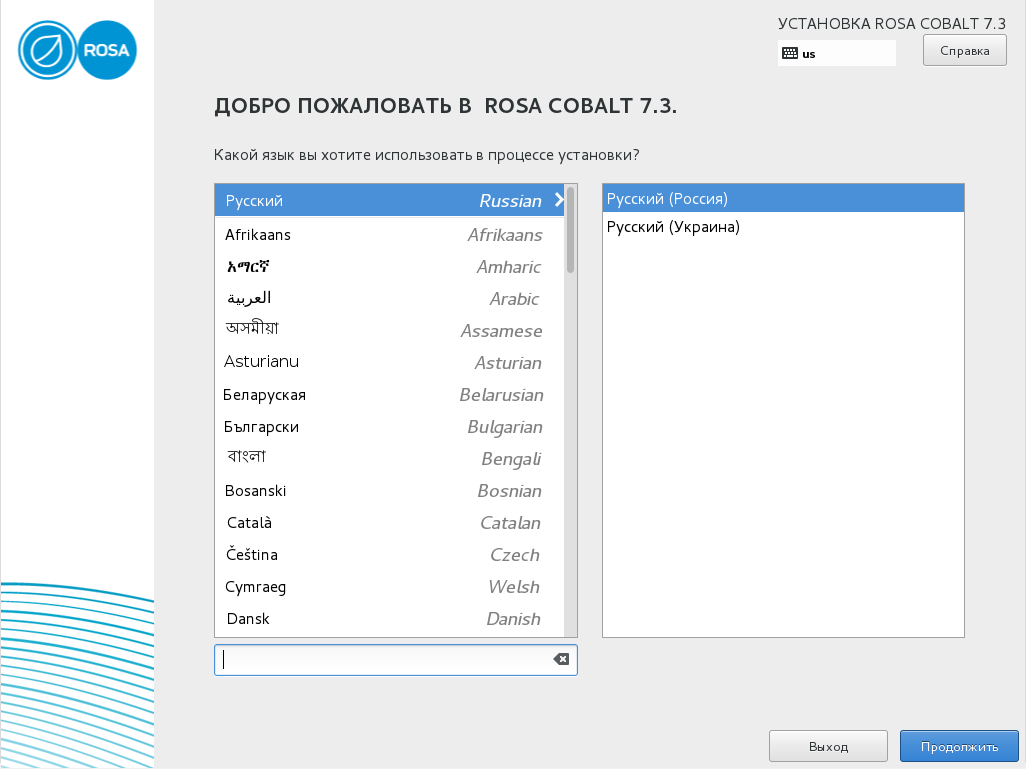
\includegraphics[scale=0.6]{0001.png}
\centering
\caption{Окно приложения TextMaker}
\end{figure}

\subsection{Панель заголовка}
В верхней части окна приложения расположена панель заголовка.

\begin{figure}[ht]

\includegraphics[scale=0.8]{0002.png}
\centering
\end{figure}
Панель заголовка показывает имя приложения и название текущего документа.

Если документ содержит ещё не сохранённые изменения, рядом с названием документа будет показана звёздочка.
\subsection{Панель меню}
Панель меню располагается непосредственно под панелью заголовка.

\begin{figure}[ht]

\includegraphics[scale=0.8]{0003.png}
\centering
\end{figure}
Эта панель содержит все команды TextMaker в виде чётко сгруппированных меню. Нажмите на пункт меню чтобы открыть меню и запустить команду.

\subsubsection{Контекстное меню}
Кроме того, доступно меню, называемое <<контекстным>>.

В этом меню можно найти разные команды, в зависимости от текущего момента. Например, если выделить текст и затем открыть контекстное меню, там будут присутствовать команды для вырезания, копирования или форматирования выделенного текста.

\begin{figure}[ht]
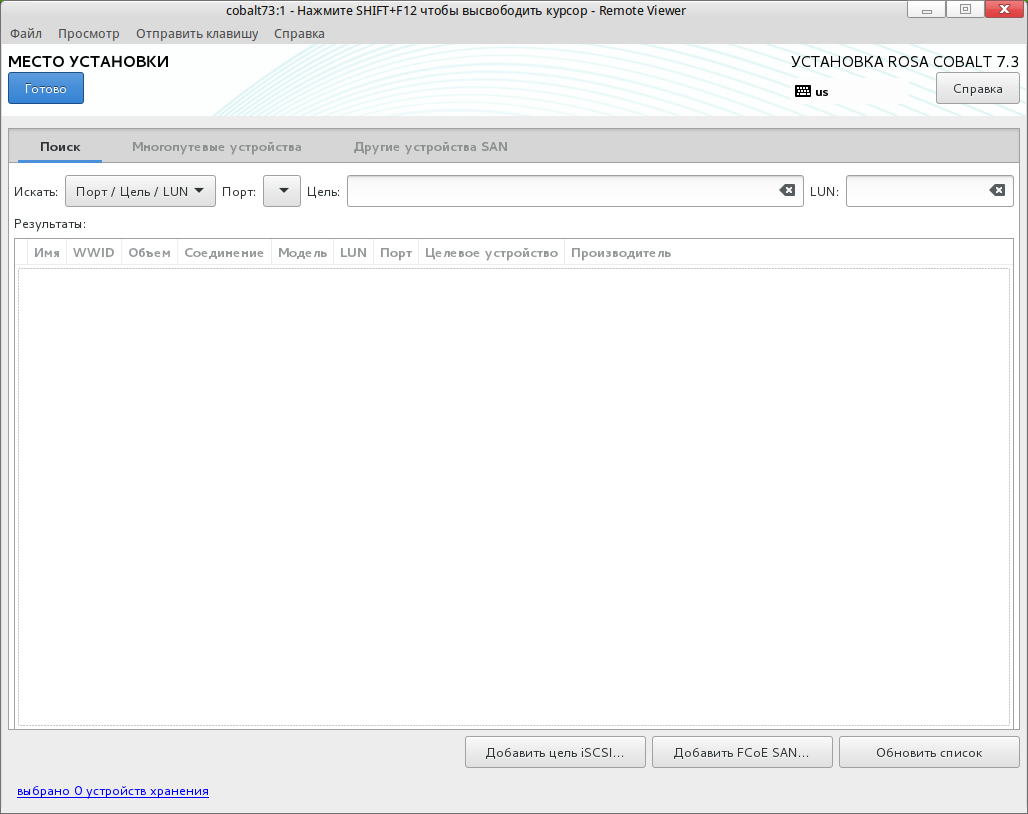
\includegraphics[scale=0.4]{0004.png}
\end{figure}

Чтобы открыть контекстное меню, обычно сначала в документе выделяют како-то элемент/текст, и затем делают щелчок правой клавишей мышки по этому элементу.

Android: в версии для Android также можно открыть контекстное меню пальцем. Коснитесь экрана и затем не отнимайте палец от экрана примерно в течение секунды.

\subsection{Стандартная панель инструментов}

Стандартная панель расположена под панелью меню. На этой панели расположены значки для наиболее часто применяемых действий. При нажатии на значок запускается соответствующая команда.


\includegraphics[scale=0.5]{0005.png}

Панели инструментов, такие, как Стандартная панель, предоставляют быстрый доступ к функциям программы. Каждый значок представляет конкретную команду. При нажатии на значок вызывается соответствующая команда.

\begin{mdframed}[backgroundcolor=blue!10]
\textbf{Совет:} если направить курсор мыши на значок (без нажатия) и удерживать в этом положении,  будет показана так называемая «всплывающая подсказка». Эта подсказка описывает действие, запускаемое при нажатии на значок. 
\end{mdframed}

В TextMaker существуют дополнительные панели инструментов, которые можно включать и отключать по желанию. Для этого либо нажмите на пункт меню \textbf{Вид>Панели инструментов} либо нажмите правой клавишей мышки по одной из видимых панелей. Будет выведено меню, в котором можно выбрать, какие панели должны показываться.

\textbf{Настройка панелей:} набор панелей по умолчанию можно изменять по желанию, а также можно создавать собственные панели. Подробности см. в разделе «Настройка панелей», который начинается на стр.566.

\subsection{Панель форматирования}
Под Стандартной панелью находится Панель форматирования. С её помощью пользователь может проверить и изменить наиболее часто используемые форматы (шрифт, полужирный шрифт, курсив и т.п.) для текущего текста.

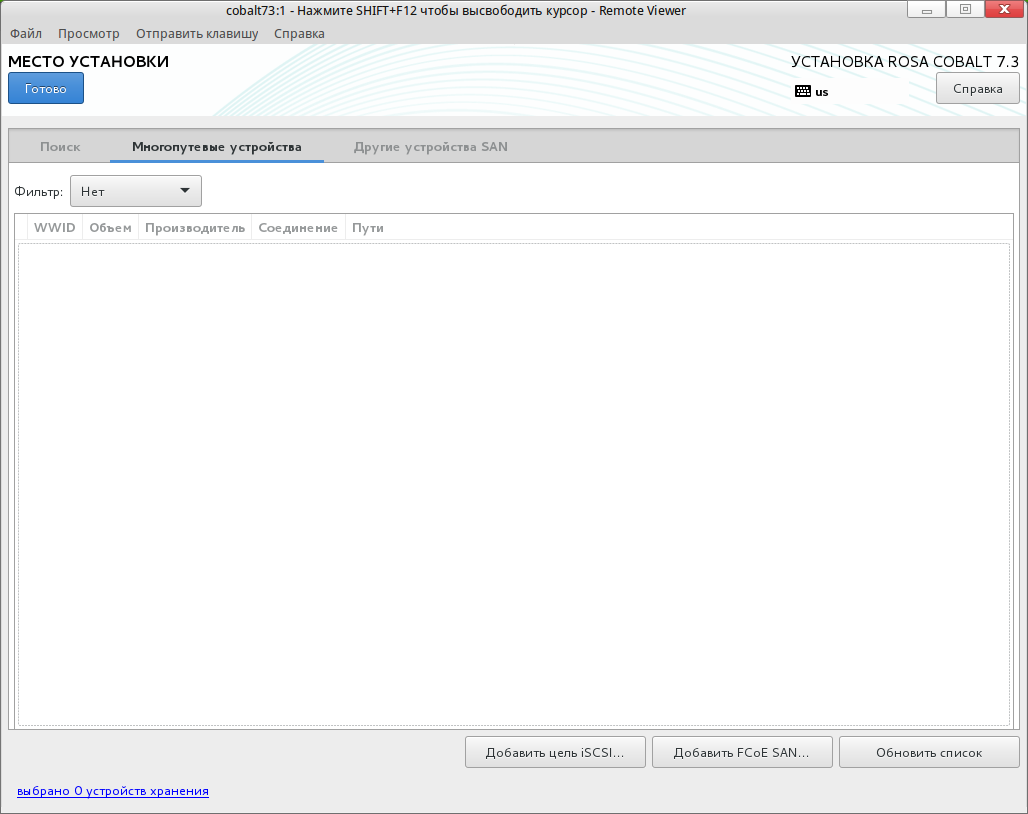
\includegraphics[scale=0.5]{0006.png}

Если фрагмент текста был выделен заранее, изменения в форматировании применяются только к этому выделенному тексту. В противном случае, изменения будут применены к тексту, который будет набираться далее.

Чтобы, например, выбрать другой шрифт, нажмите на маленькую стрелку справа от названия шрифта, чтобы открыть список шрифтов, и выберите нужный шрифт.

Другие значки на панели форматирования --- это переключатели, активируемые нажатием мышки, например, \textbf{B} для полужирного шрифта.

\subsection{Окно документа}
Окно документа, используемое для редактирования документа, занимает большую часть экрана.

Каждый документ, который открывает или создаёт пользователь, показывается в своём собственном окне, что предоставляет возможность работы с несколькими документами одновременно, и перемещать данные между этими документами.

Чтобы узнать больше о работе с окнами документов, см. раздел <<Окна документов>>, начинающийся на стр.523.

Окно документа состоит из следующих элементов:

\subsubsection{Горизонтальная линейка}
Горизонтальная линейка располагается в верхней части окна документов. Здесь показываются поля и шаг табуляции для активного параграфа, или для всех параграфов, которые могут быть выбраны в указанный момент. Единица измерения --- дюйм или сантиметр, в зависимости от системных настроек.


\includegraphics[scale=0.5]{0007.png}

Отступы и шаг табуляции не только показываются, их также можно изменять с помощью мыши. Об этом можно узнать в разделе «Отступы» (стр.80) и «Табуляция» (стр.86).

\subsubsection{Документ}
Документ как таковой занимает большую часть окна документа.

\subsubsection{Боковая панель}
Панель с правой стороны документа, называемая «боковой панелью», --- это очень полезный инструмент:

С её помощью, например, можно увидеть список всех заголовков в документе. Если сделать двойной щелчок на одному из элементов документа, TextMaker немедленно перемещается на соответствующий заголовок.

Значки на маленькой панели в верхней части боковой панели дают возможность выбрать, что именно должно показываться в боковой панели (навигатор, стили символов или параграфов).

Боковую панель можно в любое время включить или отключить с помощью пункта меню «Вид>Боковая панель». Там, где можно изменить расположение боковой панели или спрятать её, открывается подменю.

\textit{FreeOffice}: в SoftMaker FreeOffice боковая панель активируется автоматически при запуске программы, на ней показывается познавательная информация про SoftMaker Office.
Чтобы получить больше информации о боковой панели и её отдельных возможностях, см следующие разделы:
\begin{itemize}
 \item Навигация по документам с помощью боковой панели (стр.163)
 \item Стили символов и боковая панель (стр.131)
 \item Стили параграфов и боковая панель (стр.140)
\end{itemize}

\subsubsection{Строка состояния}
Строка состояния располагается в нижней части окна программы.

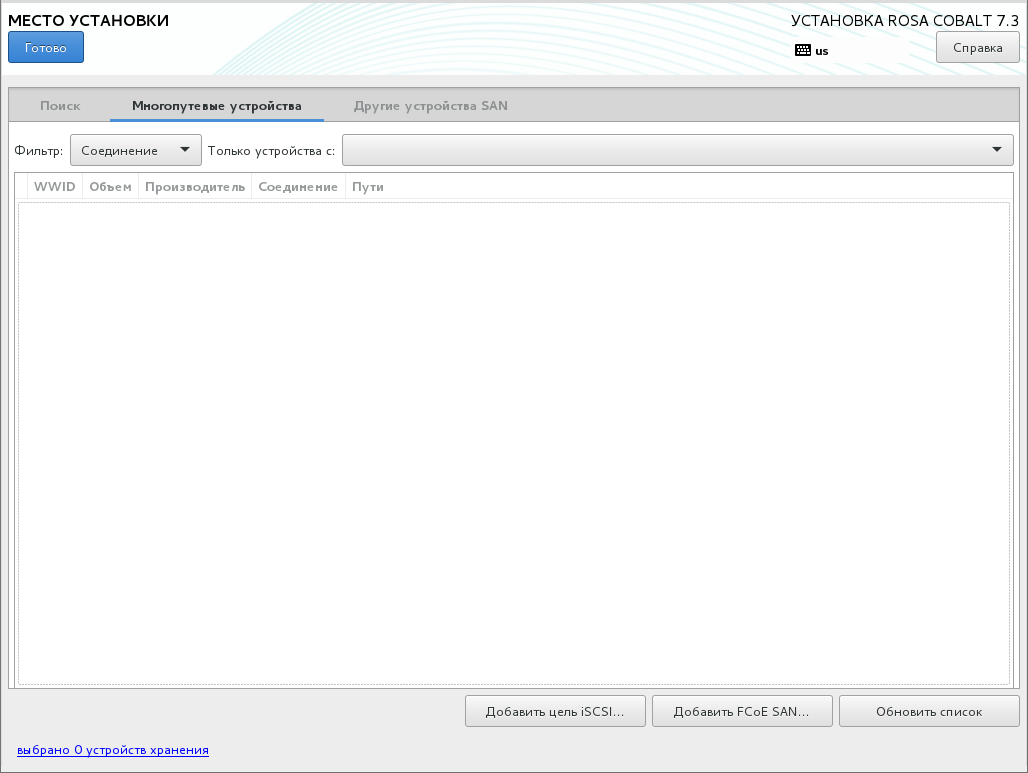
\includegraphics[scale=0.5]{0008.png}

\begin{mdframed}[backgroundcolor=blue!10]
\textbf{Подсказка:} при наведении курсора мыши на значок панели инструментов или команду меню, в строке состояния появляется краткое описания функционала этого значка или команды. 
\end{mdframed}

Кроме того, в строке состояния показывается следующая информация (слева направо):

\begin{center}
\begin{tabular}{ | m{4cm} | m{10cm} | }
\hline
 Пример & Объяснение \\ 
 \hline
 Стр.10 Кол.58 & Текстовый курсор расположен на строке 10 в колонке 58 текущей страницы. \\  
 \hline
 Раздел 1 & Текстовый курсор расположен в разделе 1 документа (см. раздел «Многоколонные макеты страниц», стр.147) \\
 \hline
 Глава 1 & Текстовый курсор расположен в главе 1 документа (см. раздел «Разделение документа на главы», стр.114). \\
 \hline
 Страница 1 из 2 & Текстовый курсор расположен на странице 1 документа, состоящего из двух страниц. \\
 \hline
 Русский & Текст в текущей позиции курсора (или текущий выделенный текст) набран на Русском языке (см. также «Настройка языка», стр.324).\\
 \hline
 Вст & Показывает, какой из режимов набора текста активен, вставка (Вст) или замена (Зам):
\textbf{Вст:} активен режим вставки — вводимый текст вставляется в существующий текст.
\textbf{Зам:} активен режим замены — вводимый текст заменяет существующий текст.
По умолчанию установлен режим вставки. Переключение между двумя режимами происходит с помощью клавиши Insert.\\
\hline
\end{tabular}
\end{center}

\section{Базовые операции}
В этой главе пользователь может познакомиться с кратким описанием наиболее важных базовых функций TextMaker. 

После этого рекомендуется обратиться к следующей главе, «TextMaker в примерах», чтобы шаг за шагом применить полученные знания на практических примерах.

\subsection{Ввод текста}
При запуске TextMaker автоматически открывается окно пустого документа, и пользователь может начинать водить текст без промедления. Не беспокойтесь, если вы умеете пользоваться пишущей машинкой, то без проблем освоите TextMaker.

\begin{mdframed}[backgroundcolor=blue!10]
\textbf{Внимание:} при работе на пишущей машинке в конце каждой строки нужно нажимать клавишу \keys{Enter}.В текстовом процессоре этого делать не нужно. Если вводимое слово не помещается в текущей строке, TextMaker автоматически перенесёт его на следующую. Клавишу \keys{Enter} нужно нажимать только в следующих случаях:
\end{mdframed}

\begin{itemize}
 \item чтобы закончить абзац
 \item чтобы ввести пустую строку
\end{itemize}

Поэтому, находясь внутри абзаца, предоставьте TextMaker делать правильные окончания строк.

\subsection{Перемещение текстового курсора}
При наборе и редактировании текста мы всегда видим мигающую чёрточку. Это так называемый текстовый курсор. При наборе текстов, буквы всегда появляются там, где расположен текстовый курсор.

Текстовый курсор можно расположить в любом месте между началом и концом документа. Для этого существуют клавиши со стрелками. Клавиши  и , например, передвигают курсор на один символ влево и вправо, соответственно.

Все доступные клавиши, применяемые для перемещения курсора:

\begin{center}
\begin{tabular}{  m{2cm} | m{12cm}  }
\hline
\keys{\arrowkeyleft} & На один символ влево \\ 
 \hline
 \keys{\arrowkeyright} & На один символ вправо\\
\hline
\keys{\arrowkeyup} & На одну строку вверх \\
\hline
\keys{\arrowkeydown} & На одну строку вниз \\
\hline
\keys{Home} & В начало строки\\
\hline
\keys{End} & В конец строки \\
\hline
\keys{Ctrl}+\keys{\arrowkeyup} & В начало текущего абзаца или, при повторном нажатии, предыдущего\\
\hline
\keys{Ctrl}+\keys{\arrowkeydown} & В следующий абзац \\
\hline
\keys{Ctrl}+\keys{Home} & В начало документа \\
\hline
\keys{Ctrl}+\keys{End} & В конец документа \\
\hline
\end{tabular}
\end{center}

Кроме того, расположить текстовый курсор в нужном месте можно нажатием мышки.

\textbf{Android}: в версии для Android также можно произвести касание пальцем в нужной позиции.

\subsection{Удаление текста}
Каждый пользователь время от времени делает опечатки, которые нужно удалять. В TextMaker это можно делать несколькими способами. 

\textbf{Удаление символов:} чтобы удалить символ, используйте клавишу \keys{BackSpace}, расположенную над клавишей \keys{Enter}. Эта клавиша удаляет символ слева от текстового курсора. Последующий текст сдвигается назад автоматически.

Также можно удалять символы в противоположном направлении: за это отвечает клавиша \keys{Delete}, которая удаляет символ не слева, а справа от текстового курсора.

\textbf{Удаление слов:} если расположить текстовый курсор перед первой буквой слова, и затем нажать сочетание клавиш \keys{Ctrl}+\keys{Del}, то это слово будет удалено. Если текстовый курсор расположен в середине слова, то это сочетание клавиш удаляет только оставшиеся буквы слова, следующие после курсора.

\textbf{Удаление возврата каретки:} пользователь также может удалить ошибочно введённый возврат каретки. Проверить это можно следующим способом: напечатайте абзац из нескольких строк и затем посредине абзаца введите возврат каретки, нажав клавишу \keys{Enter}. Дальнейший текст перемещается на следующую строчку, и абзац разделяется. В некоторых случаях, когда абзац слишком объёмный, и его нужно  разделить на два, это можно сделать намеренно. Но в данном случае это была «ошибка», поэтому --- нажмите клавишу \keys{BackSpace} для удаления возврата каретки.

\textbf{Удаление больших фрагментов текста:} вышеописанные клавиши удаления удобны для удаления небольших фрагментов текста, но удаление таким способом объёмных фрагментов текста занимает слишком много времени. Поэтому существует ещё один способ удаления текста, когда необходимый фрагмент сначала выделяется, а затем, например, нажимается клавиша \keys{Del}, для мгновенного удаления всего выделенного текста. Больше информации об этом можно найти в главе «Работа с выделениями», которая начинается на стр.59.

\subsection{Отмена изменений}
TextMaker --- программа, прощающая ошибки, и позволяющая отменить самые свежие изменения с помощью команды \textbf{Правка>Отменить}. Если пользователь, например, удалил некоторый текст, а затем решил, что этот текст нужно вернуть, всё, что ему нужно сделать, это вызвать пункт меню \textbf{Правка>Отменить}, и удаление будет отменено.

Этот способ применим не только для удалений, но практически для любого типа изменений, внесённых в документ, например, для вставки объекта в тест.

Команду \textbf{Отменить} можно применять несколько раз подряд, например, для отмены пяти последних изменений текста.

Команду \textbf{Отменить} можно также вызывать сочетанием клавишей \keys{Ctrl}+\keys{Z}.

\subsubsection{Повторение отменённых действий}
Также существует команда, действие которой противоположно команде Отмена, это команда \textbf{Правка>Вернуть}. Эта команда восстанавливает результат отменённого действия.

Для этой команды также есть сочетание клавиш: \keys{Ctrl}+\keys{Y}.

\subsection{Ввод или замена?}
Ввод текста осуществляется очень просто. Пользователь помещает текстовый курсор в нужное место и начинает печатать.

По умолчанию, в TextMaker включен режим Ввод. Если в этом режиме напечатать символ, символ вводится в существующий текст и смещает последующий текст вперёд.

Можно также переключиться в режим Замена. В этом режиме вводимый текст заменяет (перезаписывает) последующий текст.

Строка состояния всегда показывает, какой из двух режимов включен в данную минуту: \textbf{Вст} означает режим ввода, \textbf{Зам} --- пользователь работает в режиме замены.

Переключение между этими двумя режимами осуществляется с помощью клавиши \textbf{Insert}.

\subsection{Создание нового документа}
Чтобы создать новый документ, вызовите пункт меню \textbf{Файл>Новый}, или нажмите сочетание клавиш \keys{Ctrl}+\keys{N}.

\begin{figure}[ht]
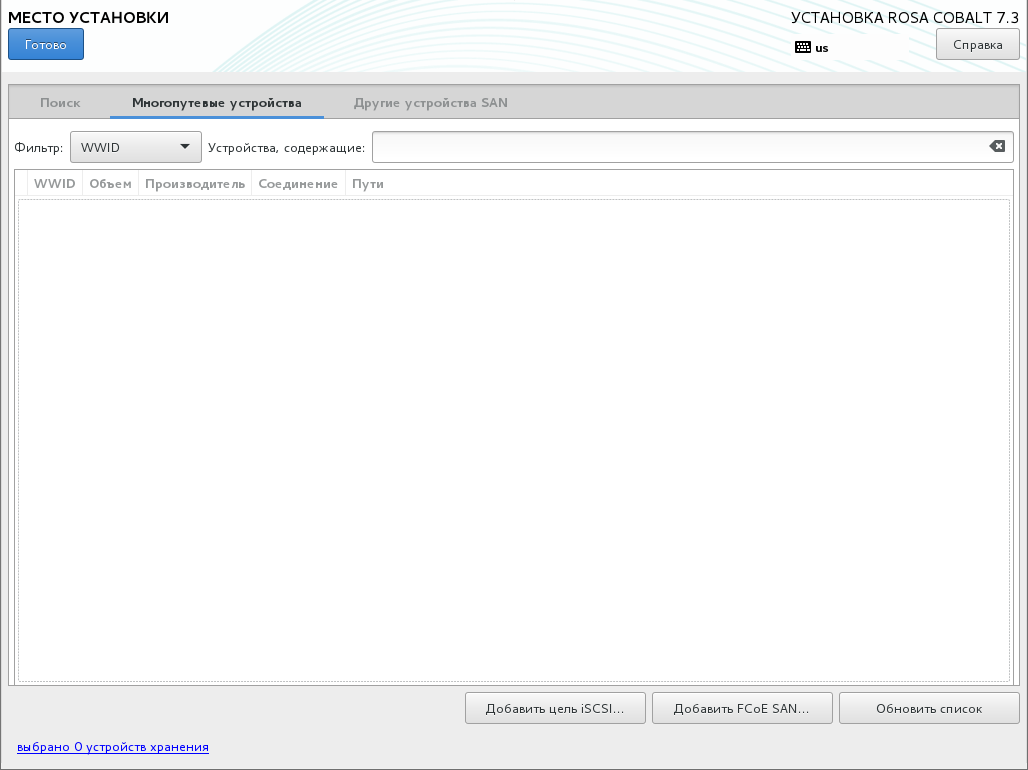
\includegraphics[scale=0.5]{0009.png}
\centering
\caption{Диалоговое окно меню Файл>Новый}
\end{figure}

Появится диалоговое окно, в котором можно выбрать шаблон для нового документа. 

Если пользователю просто нужно создать новый документ, без срочной необходимости выбора шаблона, то мы рекомендуем стандартный шаблон NORMAL.TMV.

После нажатия кнопки OK параметры нового документа будут настроены.

\subsubsection{Использование шаблонов документов}
Кроме стандартного шаблона NORMAL.TMV пользователю также доступны несколько папок, которые можно открыть двойным нажатием мыши. В папках находятся подготовленные шаблоны для писем, факсов и т.п. Далее их просто нужно наполнить содержимым.

\begin{mdframed}[backgroundcolor=blue!10]
\textbf{Совет:} в правой части диалогового окна показывается предварительный просмотр выбранного шаблона. Показ предварительного просмотра можно в любое время включить или выключить с помощью кнопки >> или << . (Эта возможность отсутствует в SoftMaker FreeOffice.) 
\end{mdframed}

Подробную информацию о работе с шаблонами документов см. в разделе «Шаблоны документов», который начинается на стр.143.

\subsubsection{Параметр «Новое окно»}
Флажок «Новое окно» в этом диалоге имеет следующее значение: при включенном флажке новый документ будет открыт в новом окне, в противном случае — текущий документ в активном окне будет закрыт, и вместо него будет создан новый документ.

\subsection{Открытие документов}
Чтобы открыть уже существующий документ, вызовите команду из пункта меню \textbf{Файл>Открыть}, или нажмите сочетание клавиш \keys{Ctrl}+\keys{O}.

Появится диалоговое окно, выглядящее примерно так: 

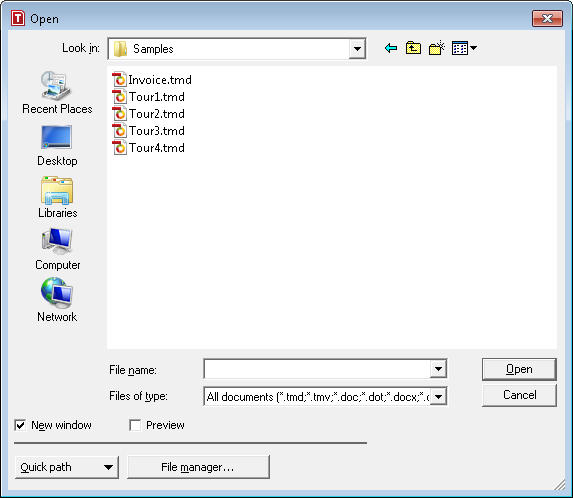
\includegraphics[scale=0.6]{00010.png}

В папке недавно использованных документов будет список всех существующих документов (отсортированных по типу файла). Чтобы выбрать файл для открытия, введите его имя вручную или просто выберите файл из списка. Затем нажмите на кнопку «Открыть».

\textbf{Новое окно}: чтобы открыть документ в новом окне, отметьте флажком параметр «Новое окно». В противном случае, текущий документ будет закрыт, и в этом же окне будет открыт новый.

\subsubsection{Открытие файлов в других форматах}
В дополнение к файлам, созданным в стандартном файловом формате TextMaker, в программе можно открывать файлы, созданные в других программах, например, в Microsoft Word. Чтобы открыть файл, созданный в другом приложении,  выберите необходимый формат файла в списке «Тип файла». 

Больше сведений по этой теме можно найти в главе «Работа с другими форматами файлов», которая начинается на стр.511.

\subsubsection{Предварительный просмотр документа}
При отмеченном параметре <<Предварительный просмотр>>, в небольшом блоке рядом с диалогом выбора файла присутствует предварительный просмотр документа.

\subsubsection{Использование быстрых путей}
С помощью кнопки «Быстрый доступ» можно создать быстрые пути для ускорения перемещения в конкретную папку при открытии или сохранении файлов. Это даёт возможность создать список наиболее часто используемых папок для быстрой навигации.

Подробности см. в разделе «Быстрый доступ», начинающемся на стр.496.

\subsubsection{Использование менеджера файлов}
\begin{mdframed}[backgroundcolor=pink!50]
\textbf{FreeOffice:} эта возможность не включена в SoftMaker FreeOffice.
\end{mdframed}

Кнопка «Менеджер файлов» открывает встроенный менеджер файлов, который показывает список документов пользователя с возможностью открыть, распечатать, просмотреть или удалить документ. Также есть возможность поиска.

Подробности см. в разделе «Менеджер файлов», который начинается на стр.498.

\subsubsection{Использование списка недавно использовавшихся файлов}
\textit{\textbf{Совет}}: в нижней части меню «Файл» находится список недавно открывавшихся файлов. Чтобы открыть такой файл снова, просто нажмите на него.

\subsection{Печать документов}
Чтобы распечатать активный документ, выберите команду \textbf{Файл>Печать} или используйте сочетание клавиш \keys{Ctrl}+\keys{P}.

Появится диалоговое окно, в котором можно указать страницы и число копий для печати. По умолчанию, печатается одна копия полного документа.

Подробности о выводе документов (печать, отправка по почте и т.д.) см. в главе «Вывод документов», начинающейся на стр.473.

\subsection{Сохранение документов}
При работе над документом рекомендуется его время от времени сохранять.

Для сохранения файла можно использовать команду \textbf{Сохранить} из меню \textbf{Файл}, или сочетание клавиш \keys{Ctrl}+\keys{S}. При использовании одного из этих двух способов, документ в активном окне сохраняется под  текущем именем.

Если у документа ещё нет имени, TextMaker автоматически предложит указать имя документа при открытии диалогового окна \textbf{Сохранить как}.

\subsubsection{Сохранение под другим именем или по другому пути}
Чтобы сохранить документ под другим названием или в другом местоположении, используйте команду \textbf{Файл>Сохранить как}. Это действие также сохраняет все внесённые в файл изменения, но пользователь должен сначала указать другое имя файла или другую папку для сохранения.

\subsubsection{Сохранение в другом формате файла}
С помощью меню \textbf{Файл>Сохранить как}, документ можно также сохранить в другом формате. Для этого, перед тем, как нажать на кнопку «Сохранить», просто выберите нужный формат файла из списка «Тип файла». Также см. главу «Работа с другими форматами файлов», начинающуюся на стр.511.

\subsubsection{Сохранение всех открытых документов}
Если у пользователя открыто несколько окон документов одновременно, для сохранения всех документов, открытых во всех окнах, можно использовать команду \textbf{Файл>Сохранить все}. TextMaker проверяет, какие из документов были изменены с момента последнего сохранения, и сохраняет только те, которые были изменены.

\subsubsection{Выход из приложения}
Чтобы выйти из программы TextMaker, используйте команду \textbf{Файл>Выход}.

Если какие-либо из открытых документов были изменены со времени их последнего сохранения, TextMaker автоматически спросит, нужно ли их сохранить.

\section{TextMaker в примерах}
Добро пожаловать в раздел «TextMaker в примерах»!

На следующих страницах, с помощью практических примеров мы представим наиболее важные возможности TextMaker.

\textbf{Внимание}: выполняя задания из примеров, по мере улучшения навыков работы, не бойтесь экспериментировать с новыми командами. Не страшно, если что-то пойдёт не так. Для каждого из заданий мы предоставляем примеры документов, чтобы в начале каждого из уроков пользователь мог открыть соответствующий документ и начал с ним работу.

\begin{mdframed}[backgroundcolor=blue!10]
\textbf{Внимание:} большинство документов для работы с заданиями были подготовлены в версии TextMaker для Windows. В других ОС некоторые элементы управления выглядят несколько иначе, но их функционал полностью идентичен. 
\end{mdframed}

\subsection{Упражнение: деловое письмо}
Готовы для первого задания? Тогда запускайте TextMaker.

\begin{mdframed}[backgroundcolor=blue!10]
\textbf{Внимание:} при первом запуске TextMaker вам будет предложено ввести имя и адрес. Эта информация требуется не для регистрации программы. TextMaker будет использовать эту информацию для автоматической персонализации шаблонов писем, факсов и т.д., входящих в состав программы. Эту информацию всегда можно изменить позже с помощью команды \textbf{Сервис>Параметры} (см. раздел «Параметры, вкладка Общие», начинающийся на стр.533).
\end{mdframed}

После запуска программы всегда появляется окно пустого документа, в котором можно сразу  начинать печатать. Тестовый курсор мигает в начале документа. Вводимый текст появляется сразу после текстового курсора, который передвигается далее вперёд. 

Для начала, давайте начнём составлять простое письмо от имени ЗАО «Рога и копыта». Просто, но профессионально. В конце данного занятия у нас будет готово полноценное деловое письмо, со всеми полагающимися атрибутами.

На этом этапе пользователь может сказать: «Не проще ли будет применить команду \textbf{Файл>Новый} и выбрать один из готовых шаблонов?» Конечно — но таким образом пользователь ничему не научится. Если вы хотите выполнять задания, им будет необходимо уделить некоторое время, но зато впоследствии вы овладеете самыми главными функциями программы и сможете немедленно изменять шаблоны для ваших нужд.

Итак, давайте начнём. Сначала напечатайте какой-нибудь текст, похожий на указанный ниже. (Копировать его буквально не обязательно, подойдёт любой текст с произвольным содержанием. )

\begin{mdframed}[backgroundcolor=blue!10]
\textbf{Важно:} нажимайте на клавишу Enter \keys{\return} только в указанных местах. При использовании текстового процессора не нужно нажимать эту клавишу в конце каждой строки, как это делается при работе с пишущей машинкой. Enter \keys{\return} необходимо нажимать только для указания конца абзаца или для вставки пустых строк.
\end{mdframed}

\begin{center}
\begin{tabular}{ | m{15cm} | }
\hline
 Дорогие клиенты! \keys{\return} \\ 
 \keys{\return} \\
 За прошедшие годы произошло много изменений. Мы наблюдали, как компании приходят и уходят, люди приезжают и уезжают, технический прогресс меняет планету. Чтобы идти в ногу со временем, ЗАО «Рога и Копыта» решило изменить свое имя на ООО «Любовь и голуби».\keys{\return} \\
 Это изменение в названии более точно отражает нашу компанию и продукты, которые мы предлагаем. Единственное отличие для вас — это смена названия.\keys{\return} \\
 \keys{\return} \\
 Мы так же, как и прежде, рады предложить вам ту же самую высококачественную продукцию по прежним и приемлемым ценам.\keys{\return} \\
 \keys{\return} \\
\hline
\end{tabular}
\end{center}

\textbf{Ошибки при вводе текста:} допущенные опечатки можно сразу же удалять, нажимая клавишу \keys{BackSpace}. Эта клавиша расположена над клавишей Enter \keys{\return}.

Если вы придерживались примера, то готовый текст должен выглядеть примерно так:

\begin{figure}[ht]
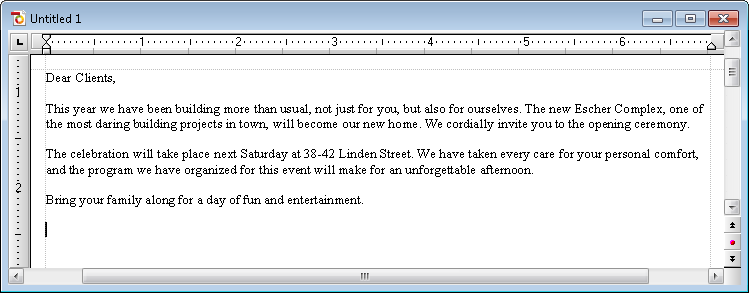
\includegraphics[scale=0.6]{00011.png}
\centering
\caption{Готовый текст}
\end{figure}

Далее, нам нужно ввести адрес над текстом нашего письма. Чтобы переместиться в начало документа, нажмите \keys{Ctrl}+\keys{Home}.

Нажмите клавишу Enter \keys{\return} семь раз, чтобы ввести несколько пустых строк. Мы создали место для адреса нашей компании, который будет введён позже. Кстати, лишние пустые строки можно удалить с помощью клавиши \keys{BackSpace}.

Далее, нажмите один раз клавишу \keys{\arrowkeyup} чтобы расположить текстовый курсор в пустой строке над текстом письма.

Теперь введите адрес и имя человека, которому адресовано письмо:

\begin{center}
\begin{tabular}{ | m{15cm} | }
\hline
1223456, Санкт-Петербург, \keys{\return} \\
Гражданская ул., дом 19\keys{\return} \\
Раскольникову Р.Р.\keys{\return} \\
\hline
\end{tabular}
\end{center}

Далее, введите дополнительные пустые строки, нажав клавишу Enter \keys{\return} одиннадцать раз, чтобы создать пустое пространство между адресом и текстом письма.

Мы создали наиболее важные элементы простого письма и на этом этапе хотим сохранить его.

\subsection{Сохранение письма-задания}
\textbf{Внимание:} подробную информацию по этой теме можно найти в разделе «Сохранение документов», который начинается на стр.36.

Чтобы сохранить текущий документ, используйте команду \textbf{Сохранить} из меню \textbf{Файл}. (Далее мы будем использовать обозначение \textbf{Файл>Сохранить}.) Вызовите эту команду следующим образом:

\textbf{\textit{Мышь}}: нажмите на кнопку \textbf{Файл} на панели меню. Откроется меню \textbf{Файл}, в котором вызвать команду \textbf{Сохранить} можно нажатием мыши.

\textbf{\textit{Клавиатура}}: для вызова команд пользователи ПК могут также использовать подчёркнутые буквы в меню. Введите подчёркнутую букву, одновременно удерживая клавишу \keys{Alt}. Например, чтобы сохранить файл, нажмите \keys{Alt}+\keys{Ф} для \textbf{\underline{Ф}айл}, а затем \keys{С} для \textbf{\underline{С}охранения}. 

Во время работы вы, возможно, заметили, что \keys{Ctrl}+\keys{S} показывается справа от команды \textbf{Сохранить}. Это является горячим сочетанием клавиш для этой команды, т.е., для вызова этой команды и сохранения документа можно также использовать данное сочетание клавиш.

Для работы с мышью также существует быстрый вызов команд --- на стандартной панели расположены значки для наиболее часто используемых команд. 


\includegraphics[scale=0.6]{00012.png}

Для сохранения документа нажмите на значок дискеты на стандартной панели инструментов (третий значок слева).

\begin{mdframed}[backgroundcolor=blue!10]
\textbf{Совет:} если направить курсор мыши на значок (без нажатия) появится текстовый блок, описывающий действие, запускаемое при нажатии на значок.
\end{mdframed}

Если стандартная панель не показывается, она, возможно, отключена. Чтобы включить её снова, вызовите команду \textbf{Вид>Панели инструментов} и отметьте галочкой \textbf{Стандартную} панель. 

\subsubsection{Диалоговое окно «Сохранить»}
Если письмо не имеет названия, при вызове пункта меню \textbf{Файл>Сохранить}, программа автоматически показывает диалоговое окно с просьбой указать имя файла. Введите имя файла в поле \textbf{Имя файла}, или, если необходимо перезаписать уже существующий файл, выберите имя из списка файлов.

Мы назовём наш документ ПИСЬМО. Поэтому, введите название «ПИСЬМО» в поле \textbf{Имя файла} и нажмите кнопку \textbf{OK} или клавишу \textbf{Enter} для подтверждения. TextMaker сохранит файл под указанным именем и автоматически присвоит ему расширение .TMD (“TextMaker document”). Таким образом мы получим полное имя файла ПИСЬМО.TMD.

В следующий раз, когда мы вызовем меню \textbf{Файл>Сохранить}, диалоговое окно уже не появится, поскольку у документа уже есть имя, и он будет немедленно сохранён под этим именем.

Кстати, выйти из диалога сохранения файла можно без выполнения команды \textbf{Сохранить}. Это можно сделать, нажав на кнопку \textbf{Отменить} вместо кнопки \textbf{OK} на контрольной панели или нажав клавишу \keys{Esc}. Этот способ доступен пользователю во всех диалоговых окнах.

\subsection{Простое форматирование}
Далее, мы приближаемся к более интересным функциям, например, к форматированию текста, а, соответственно, к применению шрифтов, визуального выделения (полужирный шрифт, курсив и т.д.), расстановке абзацев и так далее.

Сначала мы вставим строку для обратного адреса над адресом получателя, как это обычно делается для писем, отсылаемых в специальных конвертах с «окошками».

Поэтому давайте расположим курсор двумя строками выше адреса (строка 5) и введём адрес фирмы:

\begin{center}
\begin{tabular}{ | m{15cm} | }
\hline
ООО «Любовь и голуби»,  оборудование для аквариумов — г.Рыбокочинск, ул.Капитана Врунгеля, дом 2\\
\hline
\end{tabular}
\end{center}

\subsubsection{Сначала выделяем, потом форматируем}
\textbf{Внимание:} подробности выделениях можно найти в главе «Работа с выделениями», которая начинается на стр.59.

Чтобы форматировать фрагмент текста после того, как текст был введён, сначала его нужно выделить, чтобы TextMaker узнал, какую область необходимо форматировать.

Чтобы выделить строки, в которых содержится адрес, сделайте следующее:

\textbf{\textit{Мышь}}: нажимая и не отпуская кнопку мыши, перетащите курсор мыши от начала до конца текста, который нужно выделить. Кстати, существует простой способ выделить строку --- нажмите мышкой на поле слева от  строки, и вся строка целиком будет выделена.

\textbf{\textit{Клавиатура}}: пользователи, предпочитающие работу с клавиатурой, могут выделять текст, передвигая текстовый курсор, удерживая клавишу \keys{Shift}. В этом случае выделите строку адреса, с помощью клавиши \keys{Home} поместив курсор перед первым символом и затем нажав сочетание клавиш \keys{Shift}+\keys{\arrowkeydown}.

\begin{mdframed}[backgroundcolor=blue!10]
\textbf{Android:} обратите внимание, что в версии для Android выделение текста производится другим способом. Подробности см. в разделе «Выделение текста и объектов» (стр.59).
\end{mdframed}

После того, как мы выделили строку адреса, можно изменять размер шрифта. Для этого используйте панель форматирования, где находятся все наиболее часто используемые команды форматирования. Если эта панель не показывается, вызовите команду \textbf{Вид>Панели инструментов} и отметьте параметр \textbf{Форматирование}.

\subsubsection{Панель форматирования}
\textbf{\textit{Внимание}}: подробную информацию о панели форматирования можно найти в главе «Форматирование символов» (начинается на стр.67) и «Форматирование абзацев» (начинается на стр.79).


\includegraphics[scale=0.6]{00013.png}

Размер шрифта выделенного текста показывается справа от названия шрифта --- на иллюстрации выставлен размер в 10 пт. Нажмите мышью на маленькую стрелку справа от цифры 10 чтобы открыть список наиболее часто используемых  размеров шрифтов. Выберите из списка «8».

Теперь выберем другой тип шрифта. Для этого нажмите на стрелку справа от шрифта и выберите в списке Times New Roman. Если этот шрифт не был установлен, выбирайте любой понравившийся шрифт.

После внесения этих изменений панель форматирования будет выглядеть таким образом:


\includegraphics[scale=0.6]{00014.png}

Был установлен шрифт Times New Roman размером 8 пт.

Далее нам нужно выделить город и почтовый индекс адресата полужирным шрифтом. Выберите строку с городом и индексом в адресе получателя и затем нажмите на букву \textbf{B} на панели Форматирования --- или нажмите сочетание клавиш \keys{Ctrl}+\keys{B}. Шрифт строки станет полужирным.

Кстати, выделение текста курсивом делается так же просто, с помощью значка \textit{I} или сочетания клавиш \keys{Ctrl}+\keys{I}; подчёркнутый шрифт форматируется с помощью значка \underline{U} или сочетания клавиш \keys{Ctrl}+\keys{U}. Чтобы сделать обратные  изменения, применяются те же самые средства.

В итоге, адреса получателя и отправителя должны выглядеть примерно таким образом:

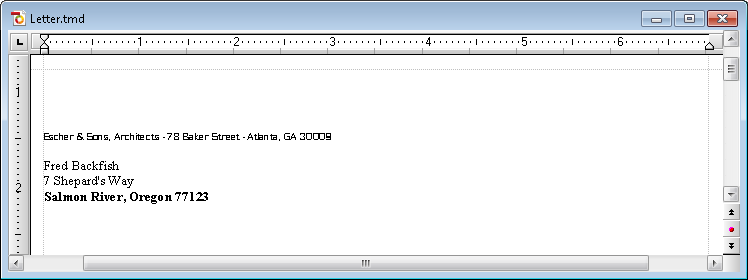
\includegraphics[scale=0.6]{00015.png}

Теперь снова необходимо сохранить наш документ с помощью \textbf{Файл>Сохранить}.

\subsection{Если что-то пошло не так…}
\textbf{Внимание:} подробную информацию по этой теме можно найти в разделе «Отмена изменений», который начинается на стр.31.

Как мы видели в предыдущем задании, снять полужирное форматирование можно, снова применив этот атрибут шрифта к тексту, уже выделенному полужирным.

В TextMaker есть дополнительная, очень удобная возможность отмены самых свежих изменений с помощью команды \textbf{Правка>Отменить}. Например, если текст был форматирован с помощью другого шрифта, всё, что нужно сделать --- это вызвать меню \textbf{Правка>Отменить}, и изменения будут отменены.

Этот способ применяется не только для форматирования, но также практически для вех типов изменения — например, можно отменить ввод абзаца или удаление текста.

Команду \textbf{Отменить} можно последовательно применять столько раз, сколько необходимо. Например, вызовите её пять раз, чтобы отменить пять последних внесённых изменений.

Кстати, эту крайне необходимую команду можно вызвать с помощью сочетания клавиш \keys{Ctrl}+\keys{Z}.
Также существует команда, противоположная по действию --- это команда \textbf{Правка>Вернуть} (сочетание клавиш \keys{Ctrl}+\keys{Y}). Эта команда восстанавливает последнее отменённое действие. Таким образом, можно отменить отмену действия.

\subsection{Открытие файлов}
\textbf{Внимание}: подробности по этой теме см. в разделе «открытие документов», который начинается на стр.33.

Теперь мы откроем файл с примером TOUR 1.TMD, прилагающийся к программе. В нём содержится наш документ-задание в таком виде, в каком он должен выглядеть на этом этапе нашей работы.

Чтобы открыть документ, вызовите команду \textbf{Файл>Открыть} из меню или с помощью сочетания клавиш \keys{Ctrl}+\keys{O}. 

Сначала перейдем в папку, где лежат документы-примеры. Чтобы её найти, выполните следующие действия:
\begin{itemize}
 \item В ОС Windows 7 или более поздних, перейдите в папку пользователя. Дальше, перейдите в папку MY DOCUMENTS \textbackslash SOFT MAKER \textbackslash SAMPLES.
 \item В Windows XP перейдите в папку MY DOCUMENTS \textbackslash SOFT MAKER \textbackslash SAMPLES.
 \item В Linux перейдите в домашний каталог пользователя и оттуда --- в каталог SOFT MAKER/SAMPLES.
 \item На устройстве Android прейдите в папку SOFT MAKER/SAMPLES на карте SD. В этой папке найдите TOUR 1.TMD и сделайте двойное касание по файлу для его открытия.
\end{itemize}

\subsection{Настройка верхнего колонтитула письма}
Конечно, нашему письму необходима достойно выглядящая «шапка», с названием компании большим шрифтом и, возможно, с описанием, какие продукты или услуги предлагает наша компания.

За работу! С помощью сочетания клавиш \keys{Ctrl}+\keys{Home} переместите текстовый курсор в начало документа TOUR 1.TMD, который мы только что открыли. Теперь введите:

\begin{center}
\begin{tabular}{ | m{15cm} | }
\hline
ООО «Любовь и голуби»\keys{\return} \\
Дизайн и планировка строительных проектов всех размеров. \\
\hline
\end{tabular}
\end{center}

Название компании вполне можно сделать чуть-чуть побольше размером: выберите первую строку и с помощью панели \textbf{Форматирования} выберите шрифт \textbf{Times New Roman}, размер 32 и сделайте его полужирным.

Размер 32 отсутствует в списке? Не важно, т.к. в списке присутствуют только наиболее часто используемые размеры, но нужный именно вам размер можно ввести вручную. Просто нажмите на размер, показанный в окошке на панели форматирования, введите 32 и подтвердите нажатием клавиши Enter \keys{\return}.

Кстати, для размера шрифта можно даже указать не целое значение (например, 12.6 пт), в том случае, если текст нужно уместить в ограниченное пространство.
В итоге, панель форматирования должна выглядеть таким образом:

\begin{figure}[ht]

\includegraphics[scale=0.6]{00016.png}
\centering
\caption{Установлен шрифт Times New Roman 32 пт полужирный.}
\end{figure}

Далее нам нужно форматировать шрифт во второй строке шрифтом Times New Roman 12 пт курсив. Для этого нам сначала нужно выделить текст. На этот раз мы не будем использовать панель форматирования, а вызовем \textbf{Формат>Шрифт}, чтобы познакомиться также и с этой часто применяемой командой.

Отроется диалоговое окно, в котором находятся сразу все возможности для форматирования символов.

\begin{figure}[ht]
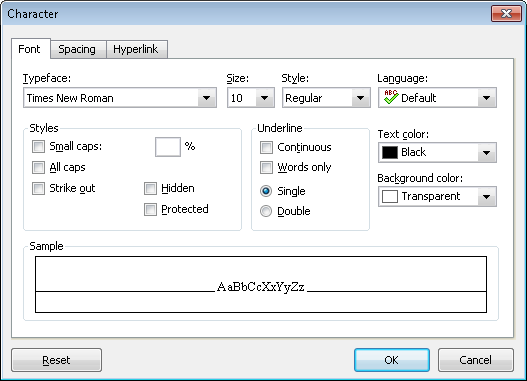
\includegraphics[scale=0.6]{00017.png}
\centering
\caption{Диалоговое окно Формат>Шрифт.}
\end{figure}

\textbf{Внимание}: подробную информацию об этом диалоговом окне можно найти в главе «Форматирование символов», которая начинается на стр.67.

Параметры диалогового окна распределены по нескольким «индексным карточкам», перейти на которые можно, нажав на вкладки в верхней части окна. Как можно видеть, в этом диалоговом окне есть вкладки \textbf{Шрифт}, \textbf{Интервал} и \textbf{Гиперссылка}. Поскольку нам нужно изменить только шрифт, мы остаёмся только на вкладке \textbf{Шрифт}.

Откройте выпадающий список «Гарнитура шрифта» нажатием на маленькую стрелку справа от названия шрифтов, и выберите шрифт Times New Roman. Затем выберите размер 12 пт в окошке справа от окошка с названиями шрифтов. Включите курсив, открыв выпадающий список \textbf{Стиль} и выбрав пункт \textbf{Курсив}.

Подтвердите выбранные параметры, нажав на клавишу \textbf{Enter}, затем сохраните документ.

\subsection{Выравнивание абзацев}
То, как TextMaker располагает текст между полями документа, называется «выравниванием абзацев».

Режим выравнивания абзацев изменяется с помощью команды \textbf{Формат>Абзац}. При вызове этой команды появляется диалоговое окно. Откройте список \textit{Выравнивание} во вкладке \textbf{Абзац}. Далее, выберите нужный способ выравнивания из списка.

Эту операцию можно выполнить быстрее с помощью панели \textbf{Форматирования}, на которой находятся четыре значка, на которые можно нажать мышью для смены способа выравнивания:


\includegraphics[scale=1]{00018.png} выравнивание слева


\includegraphics{00019.png} выравнивание справа


\includegraphics{00020.png} выравнивание по центру


\includegraphics{00021.png} выравнивание по ширине страницы

Теперь мы разместим название компании по центру страницы. Для этого, переместите текстовый курсор перед любым символом названия компании ООО «Любовь и голуби» и затем нажмите на значок «Выравнивать абзац по центру», на панели форматирования.

\begin{mdframed}[backgroundcolor=blue!10]
\textbf{Внимание:} действия по форматированию абзаца, т.е. все действия форматирования, которые выполняются через меню \textbf{Формат>Абзац}, всегда применяются ко всему абзацу. Так, если необходимо изменить формат отдельного абзаца, его не нужно сначала выделять. Просто разместите текстовый курсор на любую позицию внутри абзаца.
\end{mdframed}

С другой стороны, если необходимо изменить форматирование нескольких последовательно идущих абзацев, их необходимо сначала выделить. Выделение можно начинать с любого места внутри первого абзаца и закончить в любом месте последнего.

Давайте попробуем. Вызовите команду \textbf{Правка>Вернуть}, и название компании снова сдвинется к левому полю документа. Начиная с любой буквы в имени компании, удерживая мышь, перетащите выделение на следующую строку. Затем нажмите на значок выравнивания по центру на панели форматирования. Оба абзаца будут выравнены по центру.

После выполнения этих действий наше окно приложения будет выглядеть примерно таким образом:

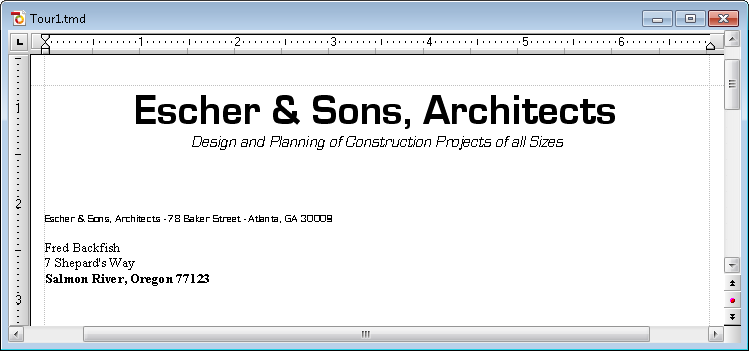
\includegraphics[scale=0.6]{00022.png}

Теперь мы можем напечатать «С наилучшими пожеланиями» внизу письма, и отправить его без лишних колебаний. Но, без сомнения, в письме есть пара элементов, которые можно сделать более привлекательными.

Поэтому давайте приступим к более тонкой отделке.

\subsection{Отступы и табуляция}
Перед тем, как продвигаться дальше, мы откроем документ TOUR 2.TMD и сравним его с нашими достижениями. В этом файле находится наш документ-пример в том виде, как он должен выглядеть на текущем этапе.

Во многие деловые письма включается строка с информацией типа: «Ваш  исходящий номер» или «Ваше письмо от» и так далее. Теперь мы вставим такую строку в наше письмо и в процессе этого познакомимся с применением отступов и табуляции.

\begin{mdframed}[backgroundcolor=blue!10]
\textbf{Внимание:} отступы вставляются с помощью клавиши \keys{Tab}. Хотя на большинстве клавиатур эта клавиша промаркирована значком \Tab, в нашем руководстве мы применяем обозначение \keys{Tab}, чтобы его было проще отличить от обозначений клавиш со стрелками.
\end{mdframed}

Теперь поместите текстовый курсор в начало строки 17 и введите следующее:

\begin{center}
\begin{tabular}{ | m{15cm} | }
\hline
Ваш исходящий номер: \keys{Tab} Ваше  письмо от: \keys{Tab} Наш исх. номер: \keys{Tab}  Наше письмо от: \keys{Tab}  Дата:\\
\hline
\end{tabular}
\end{center}

Потом отформатируйте эту строку шрифтом \textbf{Times New Roman} с размером в 8 пт.

Мы вставили отступы в текст, но ещё не определили их точного размера. Для этого нам нужно указать \textit{шаг табуляции}. По умолчанию, в TextMaker шаг табуляции равен 0,5 дюйма (1,27 см), но обычно это значение, перешедшее от пишущих машинок, не применяется.

Шаг табуляции можно настроить с помощью команды \textbf{Формат>Табуляции} или с помощью панели форматирования и \textit{горизонтальной линейки}.
\begin{figure}[ht]
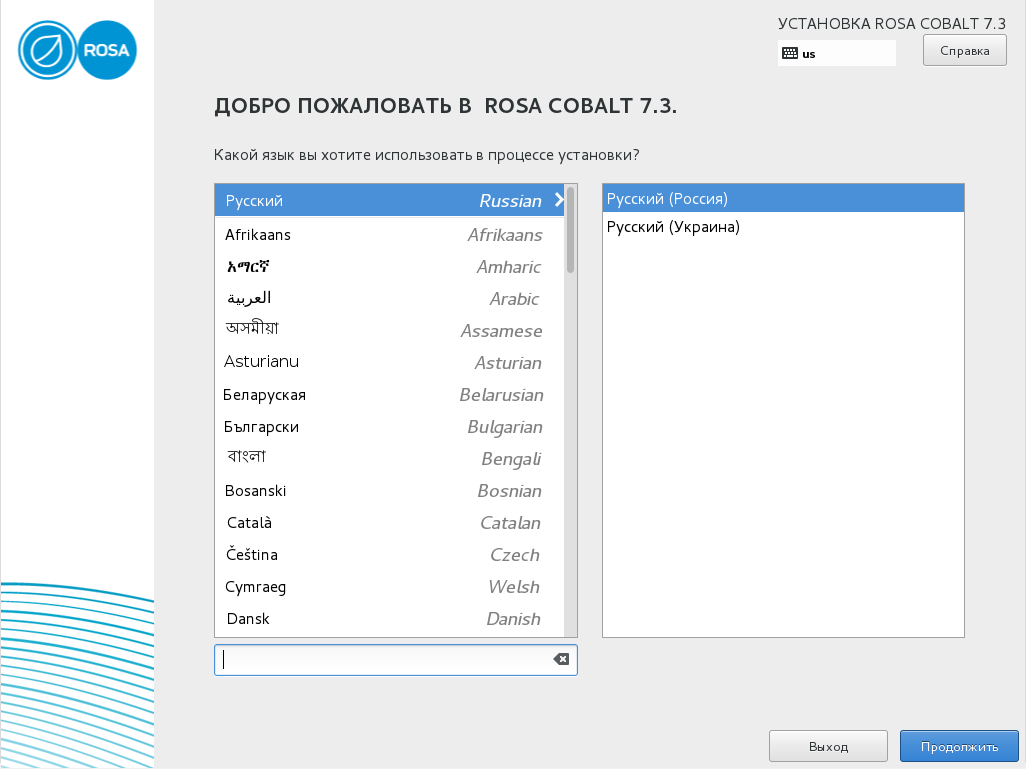
\includegraphics[scale=0.6]{0001.png}
\centering
\caption{Горизонтальная линейка}
\end{figure}

Если горизонтальная линейка в верхней части окна документа отсутствует, её нужно сначала включить с помощью команды \textbf{Вид>Горизонтальная линейка}.

Шаг табуляции настраивается следующим образом:

\begin{enumerate}
 \item \textbf{Выберите абзац, для которого нужно настроить шаг табуляции:}\\
 Если необходимо настроить шаги табуляции для нескольких абзацев, их необходимо сначала выделить, как было описано выше.\\
Выберите только что введенную строку и строку под ней, поскольку шаг табуляции для следующей строки, которую мы заполним позже, должен иметь такое же значение.
\item \textbf{Выберите нужный тип табуляции на панели Форматирования:}\\
С правой стороны панели форматирования находятся четыре различных значка выравнивания табуляции:\\

\includegraphics[scale=1]{00023.png} \textit{слева}\\

\includegraphics[scale=1]{00024.png} \textit{справа (текст заканчивается в месте табуляции)}\\

\includegraphics[scale=1]{00025.png} \textit{по центру (текст располагается по центру позиции табуляции)}\\

\includegraphics[scale=1]{00026.png} \textit{десятичное (цифры выравниваются по десятичному разделителю)}\\
Нажмите на значок левого выравнивания.
\item \textbf{Нажмите на необходимую позицию табуляции на линейке:}\\
Нажмите мышкой на (примерные) позиции в 2,54 см, 7,62 см, 10,16 см и 13,97 см чтобы установить шаги табуляции. Заметьте, как текст корректируется согласно этим параметрам.
\end{enumerate}

Заметьте, что эту же операцию можно выполнить противоположным способом, т.е. определить шаги табуляции до того, как начинать вводить текст, а затем просто ввести текст.

Линейка и текст теперь должны выглядеть примерно следующим образом:

\begin{figure}[ht]
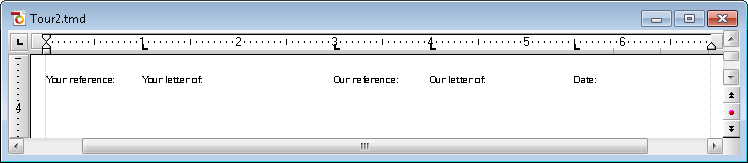
\includegraphics[scale=0.6]{00027.png}
\centering
\caption{Шаги табуляции настроены и показываются на линейке.}
\end{figure}

Если шаг табуляции не устраивает пользователя, его можно изменять прямо на линейке: сначала выделите абзац, в котором нужно изменить табуляцию, затем наведите курсор мышки на указатель шага табуляции и перетащите его на новую позицию на линейке. Не забывайте также, что при перетаскивании указателя табуляции вниз, этот шаг табуляции удаляется.

Существует ещё один способ для установки шагов табуляции. Выделив оба абзаца, вызовите \textbf{Формат>Табуляции}. Будет открыто диалоговое окно, показывающее точные текущие значения шагов табуляции. Настройки в этом диалоге выглядят следующим образом:

\begin{center}
\begin{tabular}{ | m{6cm} | m{6cm} | }
\hline
 \textbf{Цель} & \textbf{Действие} \\ 
 \hline
 Настроить шаги табуляции & Ввести необходимое значение позиции в поле \textbf{Табуляции} и нажать на кнопку \textbf{Установить}.\\
\hline
Удалить шаги табуляции & Выбрать один из существующих шагов табуляции в списке и нажать на кнопку \textbf{Очистить}. Чтобы удалить сразу все позиции, нажать на кнопку \textbf{Очистить все}. \\
\hline
Переместить шаг табуляции & Удалить шаг табуляции и установить новый. \\
\hline
Изменить выравнивание. & Нажать на один из шагов табуляции в списке, выбрать новое выравнивание в списке \textbf{Выравнивание} и нажать на \textbf{Установить}.\\
\hline
\end{tabular}
\end{center}

Для подтверждения изменений нажмите \textbf{OK}.

\textbf{Единицы измерения:} значения в диалоговых окнах TextMaker можно вводить не только в сантиметрах*, но также и в других единицах измерения. Чтобы ввести значение в конкретных единицах, просто добавьте одно из следующих сокращений после числа:

\begin{center}
\begin{tabular}{ | m{4cm} | m{4cm} | }
\hline
 \textbf{Единица измерения} & \textbf{Объяснение} \\ 
 \hline
 см & Сантиметры\\
\hline
... & Дюймы\\
\hline
пт & Пункты \\
\hline
пи & Пики\\
\hline
\end{tabular}
\end{center}

* Единицы измерения по умолчанию зависят от региональных настроек системы.

Вернёмся к нашему письму-уроку.

Теперь, когда были настроены шаги табуляции для строки «ваш исходящий номер» и строки под ней, нам нужно заполнить вторую строку.
Переместите текстовый курсор в начало строки 18 и введите:

\begin{center}
\begin{tabular}{ | m{15cm} | }
\hline
MB (Tab) 10/29/07 (Tab) HG (Tab) 10/25/07\\
\hline
\end{tabular}
\end{center}

Можно убедиться, что поскольку ранее шаги табуляции были настроены для обеих строк, то аналогичные шаги применяются и в этой строке.

В нашем письме отсутствует значение для «сегодняшнего числа». В следующем разделе урока мы настроим TextMaker на автоматическое введение даты и таким образом познакомимся с \textit{полями}.

\subsection{Ввод дат и других полей}
Сегодняшняя дата должна быть указана в области ниже «Даты», значение которой остаётся пока что незаполненным. Естественно, мы не хотим заполнять его вручную, а оставим эту задачу для TextMaker.

После введения текста, указанного выше, введите отступ с помощью клавиши \keys{Tab} и вызовите команду \textbf{Вставить>Поле}.

\begin{figure}[ht]
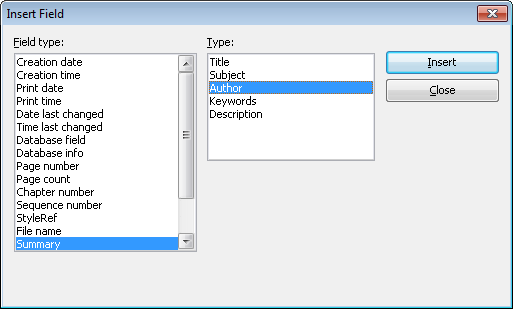
\includegraphics[scale=0.6]{00028.png}
\centering
\caption{Диалоговое окно  Вставить>Поле}
\end{figure}

Из списка Тип поля выберите поле «Дата печати». Справа, в списке Формат даты, можно выбрать формат, в котором будет вставляться дата. Выберите нужный формат и нажмите на кнопку Вставить.

TextMaker вставит текущую дату в текст, и после этого наше письмо будет выглядеть примерно таким образом:

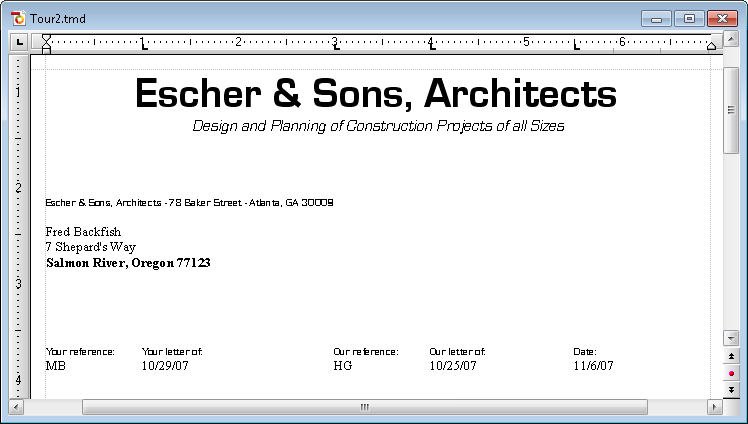
\includegraphics[scale=0.4]{00029.png}

Поля — очень удобный и практичный функционал. Во-первых, мы уже избавились от необходимости вводить текущую дату вручную, во-вторых — поле «дата печати» имеет не фиксированное, а символьное значение, автоматически обновляемое при печати документа. Поэтому, если письмо-урок будет напечатано завтра, то на этом месте будет стоять завтрашнее число.

С помощью полей можно не только вставлять дату, но также выводить текущую станицу документа, имя файла и много другой полезной информации.

Более того, с помощью полей можно вставлять поля баз данных из базы данных, как это требуется для типовых писем.

\subsection{Нижние колонтитулы}
Перед тем, как продолжать,  нам нужно открыть файл TOUR 3.TMD. В нём содержится пример документа в том виде, в каком он должен быть на этой стадии задания.

Настроить верхний и нижний колонтитулы можно для каждого документа: шапка будет печататься наверху страницы, а нижний колонтитул — внизу, на каждой странице. 

За нижние колонтитулы отвечает команда \textbf{Вставить>Нижний колонтитул}. При её вызове текстовый курсор располагается в нижней границе страницы. Это область, куда можно вводить нижний колонтитул.

Сейчас мы выберем шрифт Times New Roman 8пт перед тем, как начать вводить текст. Выберите этот шрифт с помощью панели форматирования. Теперь вводимый текст уже появится отформатированный в этом шрифте.

Давайте введём в нижнем колонтитуле адрес нашей компании и некоторую дополнительную информацию, например, сведения о банке, обслуживающем компанию. Конечно, необязательно следовать нашему образцу буквально, вы можете вводить любую информацию.

\begin{center}
\begin{tabular}{ | m{17cm} | }
\hline
ООО «Любовь и голуби»,  оборудование для аквариумов — г.Рыбокочинск, ул.Капитана Врунгеля, дом 2\\
т/ф 555-555-4242 - Факс: 555-555-4243\keys{\return}\\
\\
\hline
\end{tabular}
\end{center}

Далее, разместим обе строки нижнего колонтитула по центру, не забыв их сначала выделить, с помощью значка 
\includegraphics{00020.png} на панели форматирования, чтобы колонтитул показывался на странице примерно так:

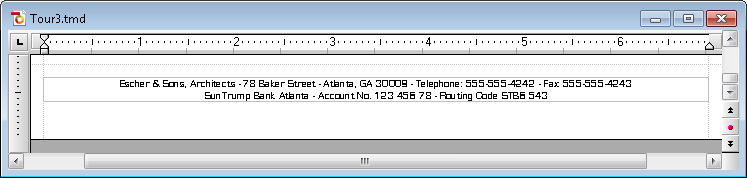
\includegraphics[scale=0.6]{00030.png}

Чтобы вернуться к обычному тексту после настройки колонтитула, просто нажмите мышью в любом месте текста. Если мы захотим изменить нижний колонтитул позже, всё, что нам нужно будет сделать, это нажать мышью на одной из строк колонтитула.

Пользуясь моментом, мы разместим завершающие письмо пожелания, под последней строкой письма. Введите пустую строку с помощью \keys{\return} и напечатайте:

\begin{center}
\begin{tabular}{ | m{15cm} | }
\hline
С наилучшими пожеланиями,\keys{\return}\\
\keys{\return}\\
\keys{\return}\\
\keys{\return}\\
И.И.Сидоров,\keys{\return}\\
ООО «Любовь и голуби»\keys{\return}\\
\hline
\end{tabular}
\end{center}

На этом наше письмо в основном готово. В следующей и завершающей части урока мы разместим линию над нижним колонтитулом, чтобы выделить его получше.

\subsection{Линии и границы}
\textbf{\textit{Внимание}}: подробную информацию по этой теме можно найти в разделе «Границы и линии», который начинается на стр.96.

В письме линия обычно размещается между нижним колонтитулом и основным текстом. Это очень легко сделать с помощью команды \textbf{Формат>Границы}. Её назначение — разместить границу вокруг абзаца или одиночные линии вдоль правого, левого,нижнего или верхнего края.

Чтобы разметить линию над нижним колонтитулом, нажмите на первую строку колонтитула и вызовите команду \textbf{Формат>Границы}.

Появится диалоговое окно, похожее на это:

\begin{figure}[ht]
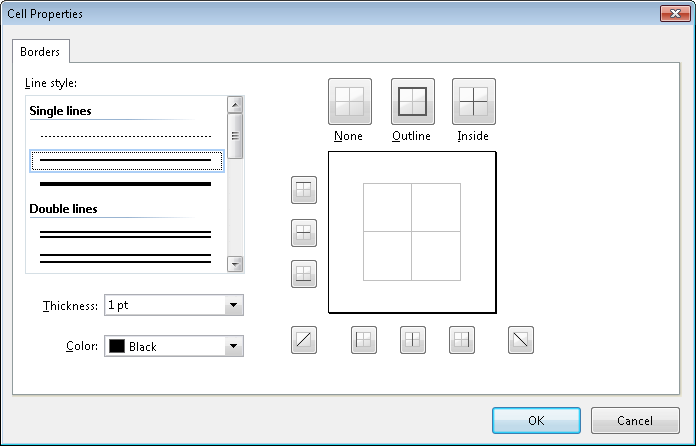
\includegraphics[scale=0.6]{00031.png}
\centering
\caption{Диалог границ}
\end{figure}

Как правило, работают с этим диалогом таким образом: сначала нужно указать какой тип линии нужен, а затем — где эту линию применить.

Соответственно, чтобы разместить линию над абзацем, нужно проделать следующее:
\begin{enumerate}
 \item Сначала выбираем тип линии, выбрав следующие параметры диалога:\\
\textbf{Стиль линии} (одиночная, двойная или пунктир)\\
\textbf{Толщина}\\
\textbf{Цвет}\\
В нашем примере мы укажем одиночную линию чёрного цвета толщиной 1пт.\\
Поскольку эти значения являются значениями по умолчанию, ничего в диалоге на этом этапе мы менять не будем.
\item Далее, укажем где применить эту линию (внизу, слева, справа и т.п.). Для этого в правой части диалога есть окошко предварительного просмотра с набором кнопок.\\
Чтобы применить границу, нажмите на соответствующую границу — прямо в окошке просмотра.\\
Или же можно добавить дополнительные линии, нажав на соответствующие границы в окошке просмотра, но нам сейчас нужна только одна.
\item Подтвердите, нажав на кнопку \textbf{OK}.
\end{enumerate}

Теперь абзац отделён тонкой чёрной линией.

Абзацы, набранные обычным текстом, можно оборудовать линиями, используя тот же самый способ, что мы применяли для колонтитулов. Кроме того, этот способ годится и для некоторых типов объектов — например, для ячеек таблицы.

\subsection{Печать письма-задания}
По желанию, вы можете теперь сделать пробную печать нашего первого сочинения. Для этого, вызовите команду \textbf{Файл>Печать} или нажмите сочетание клавиш \keys{Ctrl}+\keys{P}.

\begin{figure}[ht]
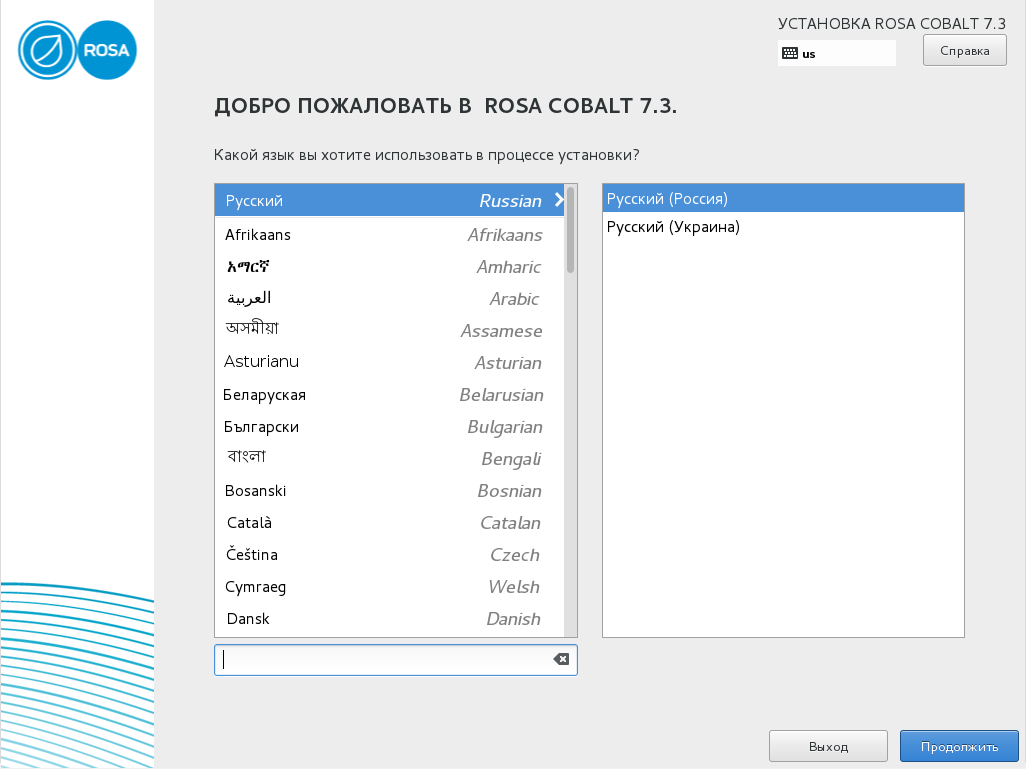
\includegraphics[scale=0.6]{0001.png}
\centering
\caption{Диалоговое окно \textbf{Файл>Печать}}
\end{figure}

В диалоговом окне «Печать» можно определить, сколько копий и каике именно страницы нужно распечатать. По умолчанию, печатается одна копия всех страниц. Подтвердите выбор с помощью кнопки OK. 

\textbf{Подсказка}: перед непосредственным процессом печати можно сделать предварительный просмотр с помощью команды \textbf{Файл>Предварительный просмотр}.

\subsection{Практическая работа закончена!}
Наш краткий обзор TextMaker в примерах на этом окончен. Пример окончательного документа можно найти в файле TOUR 4.TMD.

Теперь вы познакомились с базовым функционалом программы, и на этом этапе мы советуем уделить некоторое время дальнейшему изучению этих базовых функций. Хорошей практикой может стать, например, смена всего форматирования письма, смена шрифтов и т.д.

После этого можно углубиться в дальнейшее содержимое нашего Руководства. Руководство специально создано таким образом, чтобы пользователь мог изучить какую-то одну главу, посвящённую конкретной теме, нужной пользователю именно на текущем этапе работы. Таким образом, шаг за шагом, пользователь постигает весь функционал по мере возникающей необходимости.

Желаем продуктивной работы с TextMaker!

\section{Работа с выделениями}
Данная глава отмечает начало \textit{справочного раздела} нашего Руководства. Эта часть руководства предлагает подробное описание всех функций TextMaker, рапсределённых по тематическим главам, как это обычно и делается в справочных руководствах. 

Первая глава справочного руководства посвящена работе с \textit{выделениями}. Если нам нужно удалить, скопировать или переместить часть документа, эту часть необходимо сначала выделить. Это верно также и для объектов (рисунки, иллюстрации и т.д.).

Перед применением к тексту некоторых команд форматирования, текст необходимо также выделить. Например, для форматирования отдельного слова с помощью другого типа шрифта, это слово нужно выделить, перед тем, как устанавливать шрифт.

На последующих страницах рассказывается всё, что нужно знать при работе с выделениями. Включённые темы:

\begin{itemize}
 \item \textbf{Выделение текста и объектов}
 \item \textbf{Перемещение, удаление и копирование}
 \item \textbf{Вставка со специальным форматированием}
 \item \textbf{Вставка документов}
\end{itemize}

\subsection{Выделение текста и объектов}
Перед выполнением команды TextMaker, во многих случаях нам нужно выделить фрагмент текста (или объект), к которому должна применяться команда. Далее команда применяется к этому выделенному тексту или объекту.

В зависимости от того, в какой ОС работает TextMaker, Windows/Linux или на устройстве Android, действия по выделению текста немного отличаются. Поэтому данный раздел разделён на две части:
\begin{itemize}
 \item Выделение в версии для Windows/Linux
 \item Выделение в версии для Android
\end{itemize}

\subsubsection{Выделение в версии для Windows/Linux}
В версии TextMaker для Windows и Linux выделять можно и с помощью мыши и с помощью клавиатуры:

\textbf{\textit{Выделение с помощью мыши}}

Выделения  с помощью мыши выполняется следующим образом:
\begin{itemize}
 \item \textbf{Выделение текста}\\
 Чтобы выделить \textit{фрагмент текста} любой длины, расположите курсор мыши в начале фрагмента, затем нажмите левую кнопку, и, не отпуская кнопки, протащите до конца фрагмента.\\
Чтобы выделить слово, сделайте двойной щелчок по слову.\\
Чтобы выделить целую строку, нажмите на левом поле рядом со строкой. Можно выделить несколько строк, протащив далее курсор мыши вверх или вниз по левому полю.\\
Чтобы выделить документ целиком, нажмите и удерживайте клавишу \keys{Ctrl}, а затем нажмите мышью по левому полю (рядом с любым абзацем документа).
\item \textbf{Выделение объектов}\\
Чтобы выделить объект (рисунок, картинку и т.д.), просто нажмите на него мышью. Вокруг объекта появится рамочка, обозначающая, что объект выделен.
\item \textbf{Отмена выделения}\\
Для отмены выделения просто нажмите мышью в любом месте документа за границами выделения.
\end{itemize}

\textbf{\textit{Выделение с помощью клавиатуры}}

\begin{itemize}
 \item \textbf{Выделение текста}\\
 Переместите текстовый курсор в начало фрагмента, который нужно выделить. Нажмите и удерживайте клавишу \keys{Shift}, и двигайте текстовый курсор в любом направлении с помощью клавиш со стрелками.
 
Мы можем выделить только один символ с помощью \keys{Shift}+\keys{\arrowkeyleft} или \keys{Shift}+\keys{\arrowkeyright}, или целые страницы с помощью \keys{Shift}+\keys{PgUp} или \keys{Shift}+\keys{PgDn}.

Чтобы выделить целый документ, соответственно используется сочетание клавиш \keys{Ctrl}+\keys{Home}, после которого следует сочетание клавиш \keys{Ctrl}+\keys{Shift}+\keys{End}. Тем не менее, для этого существует более быстрый способ: вызовите команду \textbf{Правка>Выделить всё}, или сочетание клавиш \keys{Ctrl}+\keys{A}.
\item \textbf{Выделение объектов}\\
Объекты можно выделять только с помощь мыши (см. выше).
\item \textbf{Отмена выделения}\\
Для отмены выделения достаточно нажать клавишу со стрелкой.
\end{itemize}

\textbf{\textit{Выделение в версии для Android}}
В версии для Android процедура выделения выглядит несколько иначе. Можно использовать либо палец либо мышь. Выполните следующее:
\begin{itemize}
 \item \textbf{Выделение текста}\\
Самый простой способ для выделения фрагмента текста следующий:\\
двойным касанием выделите слово, которое будет служить началом выделения. Перед и после слова появятся две «метки-манипулятора», обозначающие, что слово выделено.\\

\includegraphics[scale=0.6]{00033.png}\\
Эти две метки обозначают начало и конец выделения, и также дают возможность легко расширить выделение, просто протащив метки в нужных направлениях.
\item \textbf{Выделение объектов}\\
Чтобы выделить объект (картинку, рисунок и т.д.), коснитесь его. Вокруг объекта появится рамка, обозначающая, что объект выделен.
\item \textbf{Отмена выделения}\\
Для отмены выделения коснитесь документа вне границ выделения.
\end{itemize}

\subsection{Перемещение, удаление и копирование}
Во всех операционных системах, в которых работает TextMaker, имеется крайне удобный функционал: \textit{буфер обмена}.

Буфер обмена работает следующим образом: когда мы выделяем или вырезаем что-то из документа, этот фрагмент или объект попадает в буфер обмена. Объект временно помещается в буфер обмена для  того, чтобы его можно было далее повторно вставить в любом месте документа. Таким образом, буфер обмена облегчает удаление, копирование и перемещение фрагментов текста, а также и объектов.

Все необходимые команды находятся в меню «Правка»:

\begin{center}
\begin{tabular}{ | m{4cm} | m{10cm} | }
\hline
 \textbf{Команда} & \textbf{Объяснение} \\ 
 \hline
 Удалить & При выборе фрагмента текста и дальнейшем вызове команды \textbf{Правка>Удалить}, фрагмент или объект будет удалён --- без помещения его в буфер обмена. Для более быстрого выполнения этого действия можно применять клавишу \keys{Delete}.\\
\hline
Вырезать & Команда \textbf{Правка>Вырезать} также удаляет содержимое выделения. Но не навсегда, а помещает содержимое выделения в буфер обмена, чтобы оно было доступно в любой момент позже для вставки в любом месте документа. Для вырезания также существует сочетание клавиш: \keys{Ctrl}+\keys{X}.\\
\hline
Копировать & Команда \textbf{Правка>Копировать} (сочетание клавиш \keys{Ctrl}+\keys{C}) копирует содержимое выделения в буфер обмена.\\
\hline
Вставить & Команда \textbf{Правка>Вставить} используется для вставки содержимого буфера обмена в текст. Переместите текстовый курсор на ту позицию в документе, где необходимо сделать вставку, и затем вызовите команду или нажмите \keys{Ctrl}+\keys{V}. Таким способом можно вставлять содержимое буфера обмена неоднократно.
\end{tabular}
\end{center}

В случае, если вам не до конца понятно, как буфер обмена помогает что-то удалять, копировать или перемещать, попробуйте рассмотреть всю процедуру с другой точки зрения:
\begin{itemize}
 \item \textbf{Как мне удалить текст?}\\
 Выделите фрагмент текста, и потом либо вырежьте его с помощью \keys{Ctrl}+\keys{X} для помещения его в буфер обмена, либо навсегда удалите его с помощью \keys{Delete}.
 \item \textbf{Как мне переместить текст?}\\
Выделите фрагмент текста и вырежьте его с помощью \keys{Ctrl}+\keys{X}. Потом переместите текстовый курсор на то место в тексте, куда необходимо переместить этот текст, и вставьте его с помощью \keys{Ctrl}+\keys{V}.
\item \textbf{Как мне скопировать текст?}\\
Выделите фрагмент текста и скопируйте его с помощью \keys{Ctrl}+\keys{C}. Потом переместите текстовый курсор на то место в тексте, куда необходимо скопировать этот фрагмент, и нажмите \keys{Ctrl}+\keys{V}.\\
Еси текст необходимо вставить снова, всё, что нужно сделать, это переместить курсор на следующую нужную позицию и снова нажать \keys{Ctrl}+\keys{V}.
\end{itemize}

Всё вышесказанное применимо и к объектам типа картинок и рисунков, как и способы, описанные ниже.

\subsection{Перемещение и копирование текста с помощью мыши (перетаскивание)}
Фрагмент текста, выделенный с помощью мыши, можно перетащить на другое место. С помощью этого способа, известного как «перетаскивание» (“drag and drop”), перемещение и копирование текста осуществляется очень быстро.

Выполните следующее:

\begin{enumerate}
 \item Выделите фрагмент текста.
 \item Расположите курсор мыши на выделении.
 \item Нажмите и не отпускайте левую копку мыши.
 \item С нажатой кнопкой мыши тащите выделение на необходимую позицию.
 \item После того, как вы отпустите кнопку мыши, содержимое выделения будет \textit{перемещено} в другое местоположение. А отпустив кнопку мыши при нажатой клавише \keys{Ctrl}, мы \textit{копируем} выделение в новое местоположение.
\end{enumerate}

\subsection{Вставка со специальным форматированием}
В дополнение к обычным операциям буфера обмена, таким, как \textbf{Вырезание}, \textbf{Копирование} и \textbf{Вставка}, TextMaker предлагает команду \textbf{Правка>Специальная вставка}, что даёт возможность лучше контролировать то, как именно содержимое вставляется в документ.

Подробнее:

Когда информация помещается в буфер обмена с помощью команд \textbf{Правка>Вырезать} или \textbf{Правка>Копировать}, то эта информация сохраняется в буфере в нескольких форматах. Например, если был скопирован текст, то этот текст сохраняется как в форматированном виде, так и не отформатированном виде.

Обычно это нас не волнует, т.к. TextMaker автоматически выбирает нужный формат во время вставки содержимого буфера обмена в документ по команде \textbf{Правка>Вставить}. Тем не менее, при необходимости можно выбрать формат, в котором содержимое будет вставлено. Для этого и существует команда \textbf{Правка>Специальная вставка}.

Во время вызова этой команды появляется диалоговое окно со списком всех форматов, в которых была сохранена информация, находящаяся на этот момент в буфере обмена. После выбора формата и подтверждения этого с помощи кнопки \textbf{OK}, содержимое буфера будет вставлено в выбранном формате.

\subsection{Вставка документов}
\begin{mdframed}[backgroundcolor=pink!50]
\textit{FreeOffice:} эта возможность отсутствует в \textit{SoftMaker FreeOffice}.
\end{mdframed}

С помощью команды \textbf{Вставить>Документ} можно в текущий документ вставить отдельный документ TextMaker.

Внимание: объекты с рамками (например, текстовый фрейм или текстовая рамка, фреймы рисунков и т.д.) \textit{не будут} импортированы.

Выполните следующее:
\begin{enumerate}
 \item Переместите текстовый курсор на ту позицию в документе, куда необходимо вставить другой документ.
 \item Вызовите команду \textbf{Вставка>Документ}.
 \item Будет открыто диалоговое окно, в котором можно выбрать документ для импорта.
 \item Подведите выбор с помощью кнопки OK.
\end{enumerate}

Выбранный документ будет вставлен.

\section{Форматирование символов}
С помощью команды \textbf{Формат>Шрифт} можно изменить внешний вид одного или более символов в документе.

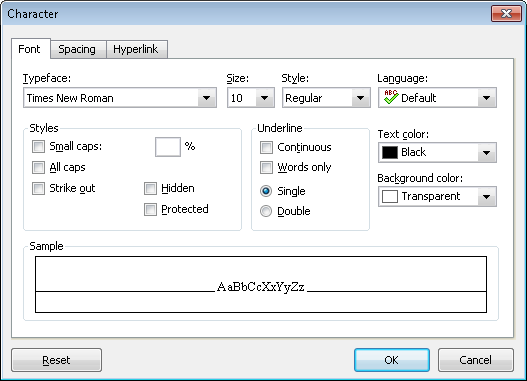
\includegraphics[scale=0.6]{00034.png}

Параметры в диалоге \textbf{Формат>Шрифт} распределены по нескольким вкладкам, перемещаться между которыми можно с помощью нажатий мыши.
\begin{itemize}
 \item Вкладка \textbf{Шрифт}\\
Используется для выбора гарнитуры и размера шрифта, стилей (полужирный, курсив и подчёркнутый), цветов текста и языка.
\item Вкладка \textbf{Интервал}\\
Используется для изменения таких свойств, как надстрочный/подстрочный формат, межсимвольный интервал, шаг печати и кернинг.
\item Вкладка \textbf{Гиперссылка}\\
Используется для вставки и редактирования гиперссылок (т.е. веб-страниц). Информацию по этой теме можно найти в разделе «Создание ссылок», который начинается на стр.468.
\end{itemize}

\textbf{Изменение формата символов}\\
Существует два способа изменить формат символов:
\begin{itemize}
 \item \textit{После того, как был введён текст}, его можно изменить, выделив нужный текст, вызвав команду \textbf{Формат>Шрифт} и внеся необходимые изменения.
 \item \textit{По мере ввода текста}, его можно изменять, вызывая команду \textbf{Формат>Шрифт}, и продолжая печать далее. С момента, например, выбора другого шрифта, вводимый текст будет форматирован этим шрифтом, до того момента, когда его снова понадобится изменить.
\end{itemize}

Дополнительная информация по теме форматирования символов представлена на следующих страницах.

\subsection{Гарнитура и размер шрифта}
Чтобы изменить гарнитуру и/или размер шрифта, сделайте следующее:
\begin{enumerate}
 \item Выделите текст, который нужно изменить.
\item Вызовите команду \textbf{Формат>Символ}.
\item Перейдите на вкладку \textbf{Шрифт}.
\end{enumerate}

Теперь можно установить нужную гарнитуру и размер шрифта:
\begin{itemize}
 \item Чтобы изменить гарнитуру, откройте выпадающий список «Гарнитура», нажав на маленькую стрелку справа, и выберите нужную.
 \item Наиболее часто употребляемые размеры шрифтов представлены в списке выпадающего меню «Размер». Можно выбрать один из представленных размеров или же вести другой размер вручную, при этом возможно указать и десятые доли размера, например, 12,7 пт.
\end{itemize}

Размеры шрифта традиционно указываются в пунктах (пт). Как правило, для основного текста используют размеры между 10 и 12 пт, и от 14 до 18 для заголовков. Основные заголовки могут быть ещё больше (например , 24пт).

\subsubsection{Работа с панелью Форматирования}
Гарнитуру и размер шрифта также можно изменить с помощью панели Форматирования.

\begin{figure}[ht]

\includegraphics[scale=0.6]{00035.png}
\centering
\caption{Панель форматирования}
\end{figure}

Для этого нужно выделить текст, открыть выпадающий список с гарнитурами или с размерами шрифтов и выбрать желаемые значения нажатием кнопки мыши.

\subsection{Стили шрифта}
Стили шрифта — это такие параметры выделения текста, как полужирный шрифт, курсив, подчёркнутый и т.п. 

TextMaker представляет следующие стили текста:
\begin{itemize}
 \item \textit{Курсив} — гарнитура с наклоном
 \item \textbf{Полужирный} — утолщённая гарнитура
 \item \textsc{Малые прописные (капители)} --- строчные буквы заменяются малыми прописными
 \item ПРОПИСНЫЕ --- все буквы являются заглавными
 \item \sout{Перечёркнутые} — текст перечёркнут
 \item Скрытый — текст не выводится на экран, не выводится на печать или не показывается обоих случаях (см. раздел «Скрытый текст», который начинается на стр.74)
 \item Защищённый — текст не подлежит изменению (см. раздел «Защита текста», который начинается на стр.75)
 \item \underline{Подчёркнутый} — одинарное или двойное подчёркивание текста. Линия может быть непрерывной или подчёркивать только слова.
 \item Надстрочный (например, x\textsuperscript{2}) или подстрочный (H\textsubscript{2}O) — эти стили можно найти в следующей вкладке (см. раздел «Надстрочный и подстрочный шрифты», начинающийся на стр.71)
 \item Цвет текста и цвет фона — см. следующий раздел
 \item Язык — при необходимости можно также указать язык для фрагмента текста (это требуется только если в документе используется больше одного языка, см. раздел «Языковые параметры», начинающийся на стр.324)
\end{itemize}

\subsubsection{Применение стилей к тексту}
Чтобы применить стиль к тексту, вызовите команду \textbf{Формат>Шрифт} и переключитесь на вкладку \textbf{Шрифт}.

Чтобы включить полужирный или курсив, откройте выпадающий список \textbf{Стиль} (справа от выбора размера) и выберите нужный стиль из списка: Обычный, \textit{Курсив}, \textbf{Полужирный} или \textit{\textbf{Полужирный курсив}}.

Чтобы применить другие стили, включите или отключите их, отметив галочкой соответствующие параметры в диалоге \textbf{Стили}.

Пользователь не ограничен только одним стилем, можно применять сочетания стилей, хотя не все сочетания возможны.

\subsubsection{Использование панели Форматирования}


\includegraphics[scale=0.6]{00035.png}

Нажмите на значок того стиля, который нужно применить или отменить: \textbf{B} — полужирный, \textit{I} — курсив, \underline{U} — непрерывное подчёркивание.

\begin{mdframed}[backgroundcolor=blue!10]
\textbf{Совет:} для применения этих стилей также существуют сочетания клавиш: \keys{Ctrl}+\keys{B}, \keys{Ctrl}+\keys{I} и \keys{Ctrl}+\keys{U}, соответственно.
\end{mdframed}

\subsection{Цвет текста}
Можно указывать цвет как для текста, так и для его фона.

Для этого:
\begin{enumerate}
 \item Выделите нужный текст.
 \item Вызовите команду \textbf{Формат>Шрифт}
 \item Перейдите на вкладку Шрифт.
\end{enumerate}

Теперь можно выбрать желаемый цвет текста из списка \textbf{Цвет текста}.

Также можно указать цвет фона в списке \textbf{Цвет фона}. По умолчанию, фон для текста является прозрачным. Если указать цвет для фона, то эффект текста на цветном фоне будет аналогичным эффекту цветного маркера на бумаге.

\subsubsection{Примечания}
\begin{itemize}
 \item Цвет текста по умолчанию с названием «Автоматический» имеет особенное свойство: текст, форматированный в этом цвете, обычно показывается чёрным. Тем не менее, если изменить цвет фона на какой-нибудь очень тёмный цвет, цвет текста автоматически сменится на белый (чтобы сохранить читаемость текста).
 \item Если никакой из предложенных в списке цветов не устраивает пользователя, всегда можно создать свой цвет. Для этого нажмите на кнопку «Задать цвет» (последний пункт в списке цветов). См. также раздел «Свойства документа, вкладка \textbf{Цвета}», который начинается на стр.556.
 \item Цвет текста также можно изменять с помощью списка цветов 
\includegraphics[scale=0.6]{00036.png} на панели \textbf{Форматирования}. Нажмите на этот список (в правой части панели) и выберите нужный цвет.
 \item Непосредственно справа от цвета текста находится элемент для Выделения цветом, также в виде раскрывающегося списка. С его помощью можно добавить цвет \textit{выделения} для выбранного теста, по аналогии с выделением цветным маркером.\\
 Внимание: эта возможность \textit{не} является аналогичной цвету фона, описанному выше. Это --- \textit{дополнительный} цвет, который можно применить только с помощью данного выпадающего писка на панели. Логику этого функционала можно оспаривать, но именно в таком виде он присутствует в Microsoft Word, поэтому в TextMaker он реализован точно так же, в интересах совместимости.
\end{itemize}

\subsection{Надстрочный и подстрочный шрифты}
Расположение шрифта выше (x\textsuperscript{2}) или ниже (H\textsubscript{2}O) базовой линии шрифта называется надстрочным или подстрочным написанием (или верхним или нижним индексом).

Выделите текст, вызовите команду \textbf{Формат>Шрифт}, перейдите на вкладку \textbf{Интервал}, и отметьте галочкой параметр «Надстрочный» или «Подстрочный».

При желании, можно указать размер сдвига ниже или выше базовой линии, введя процентное значение в окошке «Позиция». Кроме того, можно указать точное процентное уменьшение размера надстрочного/подстрочного шрифта в окошке «Размер». Если, например, пользователю необходимо, чтобы размер  надстрочного/подстрочного шрифта соответствовал размеру нормального текста, то нужно отметить 100\%.

\textbf{\textit{Совет}}: для установки надстрочного и подстрочного шрифта доступны также следующие сочетания клавиш: \keys{Ctrl}\keys{Shift}\keys{NumLock+} (клавиша плюс, расположенная на вспомогательной цифровой клавиатуре) для надстрочного шрифта, \keys{Ctrl}\keys{Shift}\keys{NumLock-} для подстрочного, \keys{Ctrl}\keys{Shift}\keys{NumLock*} --- для удаления либо того либо другого.

\subsection{Межсимвольный интервал и плотность расположения знаков}
TextMaker также даёт возможность изменять межсимвольный интервал и плотность расположения знаков.

Интервал — это расстояние по горизонтали между символами. Значение меньше 100\% приближает символы друг к другу; значение больше 100\% --- отдаляет.
Параметр «плотность расположения» влияет на ширину букв шрифта, а не на расстояние между ними.

Для изменения этих параметров вызовите \textbf{Формат>Шрифт}, перейдите на вкладку \textbf{Интервал} и введите нужное значение в поле \textbf{Межсимвольный интервал} или \textbf{Плотность расположения}.

\textit{\textbf{Внимание}}: изменение плотности расположения для \textit{внутренних} шрифтов некоторых принтеров игнорируется на выводе печати.

\subsection{Кернинг}
Некоторые пары букв выглядят лучше, если интервал между ними немного уменьшить или немного увеличить. Такое действие, называемое «кернинг», в TextMaker можно выполнять автоматически.

С помощью этой иллюстрации можно лучше понять, что такое кернинг:

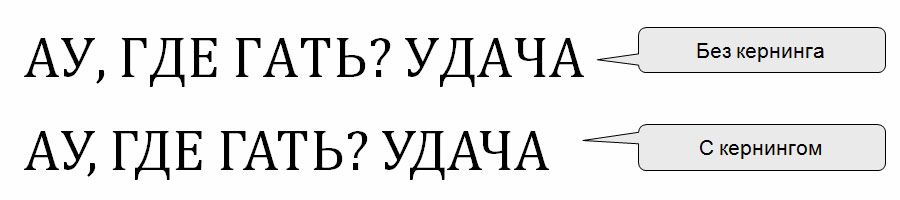
\includegraphics[scale=0.3]{00037.png}

Чтобы включить кернинг, выберите нужный текст, выберите команду \textbf{Формат>Шрифт}, перейдите на вкладку \textbf{Интервал} и активируйте параметр \textbf{Использовать кернинг}.

С этого момента TextMaker автоматически будет настраивать интервалы между буквами там, где это улучшит внешний вид текста.

\textit{\textbf{Внимание}}: не все гарнитуры предоставляют \textit{информацию о кернинге} в данных шрифтов, нужную для программного определения того, какие именно пары букв нужно настраивать, и как. Почти все наборы шрифтов, опубликованные \textbf{SoftMaker}, включают в себя исчерпывающую информацию о кернинге.

\subsection{Перенос форматирования}

\begin{mdframed}[backgroundcolor=pink!50]
\textbf{\textit{FreeOffice}:} эта возможность отсутствует в \textbf{SoftMaker} \textit{\textbf{FreeOffice}}.
\end{mdframed}

С помощью команды \textbf{Формат>Перенести форматирование} можно быстро применить формат шрифта (гарнитура, размер, стиль и др) к другим символам.

Для этого сделайте следующее:
\begin{enumerate}
 \item Выберите символ, формат которого нужно изменить. Можно также выбрать несколько символов, но их формат должен быть одинаковый.
 \item Вызовите команду \textbf{Формат>Перенести форматирование}.\\
Курсор мыши примет форму маленькой кисти: 
\includegraphics[scale=1]{00038.png}
\item Удерживая левую кнопку, протащите мышь по символам, формат которых нужно перенести.\\
\textit{\textbf{Совет}}: если вышеуказанное действие проделать при нажатой клавише \keys{Ctrl}, то будет перенесён не только формат символов, но и формат абзаца.
\item Если необходимо перенести форматирование неоднократно, повторите шаг 3 столько раз, сколько это нужно.
\item Закончив, снова вызовите команду \textbf{Формат>Перенести форматирование} или просто нажмите клавишу Esc.
\end{enumerate}

\subsection{Скрытый текст}
TextMaker даёт возможность скрывать текст. Обычно, скрытый текст показывается на экране, но не выводится на печать.

Скрытый текст идеально подходит для комментариев или примечаний, которые необходимы в тексте, но не нужны в печатном варианте документа.

\subsubsection{Скрытие текста}
Чтобы скрыть текст, проделайте следующее:
\begin{enumerate}
 \item Выделите текст, который необходимо скрыть.
 \item Вызовите команду \textbf{Формат>Шрифт}.
 \item Отметьте параметр «Скрытый».
\end{enumerate}

Теперь текст является скрытым. По умолчанию, он будет показываться на экране, но будет отсутствовать при печати документа.

\subsubsection{Показ/печать скрытого текста}
По умолчанию, скрытый текст виден на экране, но не показывается на отпечатанной странице. Тем не менее, в свойствах документа можно указать, нужно ли показывать скрытый текст на экране, и нужно ли скрытый текст печатать.

Для этого, вызовите команду \textbf{Файл>Свойства} и переключитесь на вкладку \textbf{Вид}. В разделе «Скрытый текст» присутствуют следующие параметры:
\begin{itemize}
 \item \textbf{Показать скрытый текст}\\
Этот параметр контролирует видимость скрытого текста на экране.\\
Этот параметр отмечен по умолчанию, и по умолчанию скрытый текст виден на экране. Скрытый текст выделяется нижним подчёркиванием в виде точек, так чтобы его можно было отличить от обычного текста.\\
Если отключить этот параметр, скрытый текст не будет виден на экране.
\item \textbf{Печатать скрытый текст}

Параметр \textbf{Печатать скрытый текст} контролирует вывод скрытого текста на печать вместе с обычным текстом.\\
По умолчанию, этот параметр не отмечен, и скрытый текст отсутствует в отпечатанном документе.\\
Этот параметр нужно отметить, если необходимо вывести скрытый текст на печать.
\end{itemize}

\subsubsection{Удаление свойства «скрытый»}
Если пользователю необходимо удалить форматирование текста как «скрытого», нужно сделать следующее:
\begin{enumerate}
 \item Убедитесь, что параметр «показать скрытый текст» отмечен в свойствах документа (см. выше), так что скрытый текст виден при просмотре документа на экране.
 \item Выделите скрытый текст, вызовите команду \textbf{Формат>Шрифт} и снимите галочку с параметра «Скрытый» во вкладке \textbf{Шрифт}.
\end{enumerate}
Текст  более не является скрытым.

\subsection{Защита текста}
Фрагмент текста можно защитить от изменений или удаления.
\subsubsection{Защита текста}
Чтобы защитить текст, выполните следующее:
\begin{enumerate}
 \item Выделите текст, который нужно защитить.
 \item Вызовите команду \textbf{Формат>Символ}.
 \item Переключитесь на вкладку \textbf{Шрифт}.
 \item Отметьте параметр \textbf{Защищённый}.
\end{enumerate}
Текст, защищённый таким образом, нельзя изменять. Если поместить текстовый курсор в такой текст и попытаться что-то напечатать или удалить, эти действия не будут иметь никакого эффекта.

\begin{mdframed}[backgroundcolor=blue!10]
\textbf{\textit{Важное примечание:}} если выделить фрагмент текста, включающий в себя скрытый текст, и удалить этот фрагмент, то защищённый текст, входящий в этот фрагмент, будет удалён вместе с обычным текстом. Защита предотвращает редактирование или удаление только в границах скрытого текста.
\end{mdframed}

\subsubsection{Удаление свойства «защищённый»} 
Чтобы удалить защиту с текста, выделите нужный фрагмент защищённого текста, вызовите команду \textbf{Формат>Символ} и снимите галочку с параметра \textbf{Защищённый} во вкладке \textbf{Шрифт}.

Фрагмент текста более не защищён, и его можно удалять и редактировать.

\textbf{Удаление форматирования}

В случае, если необходимо удалить форматирование символов, в TextMaker это можно сделать быстро и просто.

Выполните следующие действия:
\begin{enumerate}
 \item Выделите нужный фрагмент текста.
 \item Вызовите команду \textbf{Формат>Стандартный} или нажмите сочетание клавиш \keys{Ctrl}+\keys{Пробел}.
\end{enumerate}

TextMaker удалит любое форматирование, ранее применённое к тексту с помощью команды \textbf{Формат>Символ} или с помощью панели \textbf{Форматирования}.

Форматирование абзаца и форматирование символов, являющихся стиля абзаца, останется нетронутым.

\begin{mdframed}[backgroundcolor=blue!10]
\textbf{Внимание:} это действие также удаляет свойства текста \textbf{Скрытый} и \textbf{Защищённый}. Соответственно, ранее скрытый текст станет видимым, а ранее защищённый текст станет возможно редактировать.
\end{mdframed}

\subsection{Изменение форматирования по умолчанию}
Стандартное форматирование можно изменить в любое время. Если, например, пользователю не нравится выбранный по умолчанию шрифт, то это можно изменить за несколько нажатий мыши.

Выполните следующее:
\begin{enumerate}
 \item Вызовите команду \textbf{Формат>Символ}.
 \item В диалоговом окне настройте желаемые параметры по своему выбору.
 \item Теперь внимание: вместо нажатия на кнопку OK, нажмите на кнопку \textbf{Установить по умолчанию}.
 \item TextMaker выведет запрос, нужно ли изменить параметры по умолчанию только для текущего документа или также и для всех последующих документов.\\
\textbf{Изменить только в этом документе:} при выборе этого параметра, изменённое форматирование по умолчанию будет применено только к текущему документу.\\
\textbf{Изменить для всех новых документов:} при выборе этого параметра, изменённое форматирование по умолчанию будет сохранено в стандартном шаблоне документа (Normal.tmv), и, соответственно, все будущие документы будут созданы на основе этих параметров.
\item Подтвердите выбор с помощью кнопки \textbf{OK}.
\item Для выхода из диалога снова нажмите \textbf{OK}.
\end{enumerate}

TextMaker сохранит выбранные параметры форматирования в качестве параметров по умолчанию.

(Для продвинутых пользователей: с технической точки зрения, TextMaker просто применяет эти параметры к стилю по умолчанию  «Обычный». См. также раздел «Стиль символов \textbf{Обычный}», стр.120.)

\section{Форматирование абзацев}
Чтобы установить форматы для абзацев, используйте команду \textbf{Формат>Абзац}.

Вот наиболее часто используемые параметры для формата абзацев:
\begin{itemize}
 \item Отступы
 \item Интервал между строками
 \item Интервал над/под абзацем
 \item Выравнивание абзацев
 \item Формат символов для всего абзаца
 \item Табуляция
\end{itemize}

Также доступны следующие дополнительные параметры:
\begin{enumerate}
 \item Маркированный список (и нумерованный список)
 \item Буквица
 \item Заливка
 \item Границы и линии
 \item Уровень разбивки
 \item Частота переносов (см. раздел «Переносы»)
 \item Принудительная разбивка перед абзацами (разрыв страницы, разрыв колонки)
 \item Контроль абзацев (не отрывать абзац от следующего и т.п.)
 \item Подавление нумерации строк
\end{enumerate}

Подробности см. далее.

Форматирование абзацев всегда применяется только к абзацам целиком. Изменения форматирования абзаца влияет на весь абзац, в котором расположен текстовый курсор. При выборе нескольких абзацев, форматирование меняется во всех выбранных абзацах.

\textbf{Изменение форматирования абзацев}

Изменить форматирование абзацев можно одним из следующих способов:
\begin{itemize}
 \item Чтобы изменить форматирование абзацев после того, как они были напечатаны, выберите нужный абзац, вызовите команду \textbf{Формат>Абзац} и сделайте необходимые изменения.
 \item Чтобы изменить форматирование абзацев во время их набора, установите нужное форматирование с помощью команды \textbf{Формат>Абзац}, без выделения. Текущий абзац будет переформатирован согласно новым параметрам. Далее эти параметры будут применяться ко всем новым абзацам, начинаемым по нажатию клавиши \textbf{Enter}, до тех пор, пока пользователь снова не изменит форматирование.
\end{itemize}

\textbf{Стили абзацев (для продвинутых пользователей):} стили абзацев --- это способ значительно сократить общий объём работы при форматировании абзацев. С их помощью можно очень быстро применить предварительно настроенные форматы. Эту информацию можно найти в главе «Стили», которая начинается на стр.123.

Единицы измерения: значения в диалоговых окошках TextMaker можно вводить в различных единицах.

\begin{center}
\begin{tabular}{ | m{4cm} | m{4cm} | }
\hline
 \textbf{Единица измерения} & \textbf{Объяснение} \\ 
 \hline
 см & Сантиметры\\
\hline
... & Дюймы\\
\hline
пт & Пункты \\
\hline
пи & Пики\\
\hline
\end{tabular}
\end{center}

\subsection{Отступы}
С помощью отступов мы изменяем правые и левые границы абзацев для сужения или расширения текста. Отступ для первой строки абзаца можно настроить отдельно.
Отступы всегда указываются относительно полей страницы. Если, например, левое поле страницы настроено на 1 см, и \textbf{Левый} отступ настроен на 1,5см, то текст будет начинаться на расстоянии в 2,5см.

\begin{mdframed}[backgroundcolor=blue!10]
\textbf{Внимание:} поля страницы указываются с помощью команды \textbf{Файл>Параметры страницы}, а \textit{не} с помощью отступов.
\end{mdframed}

Чтобы использовать отступы, поместите курсор внутрь нужного абзаца или выберите несколько абзацев. Затем вызовите команду \textbf{Формат>Абзац} и перейдите на вкладку \textbf{Абзац}.

В диалоговом поле «Отступы»  можно указать Левый отступ, Правый отступ и отступ для Первой строки. Введите нужные значение в соответствующие окошки.
Если, например, нам нужно расширить текст, то можно ввести отрицательное значение.

\subsubsection{Использование горизонтальной линейки}
Включенная горизонтальная линейка (отмеченный параметр \textbf{Вид>Горизонтальная линейка}) предоставляет удобный альтернативный способ для изменения отступов.

Отступы показывается на линейке следующим образом:

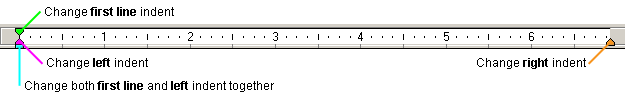
\includegraphics[scale=0.6]{00039.png}

Чтобы изменить отступ, сначала выберите абзац(ы), который нужно изменить, далее нажмите мышью на один из треугольных манипуляторов на линейке (см. картинку выше), и удерживая кнопку мыши, перетащите его на нужную позицию.

Изменяя \textbf{Левый} отступ, внимательно выбирайте нужный треугольник --- за левый отступ отвечает \textit{нижний} треугольник. Соответственно, \textit{верхний} манипулятор-треугольник отвечает за отступ только для \textbf{Первой} строки. \textit{Прямоугольный} манипулятор отвечает за изменение \textbf{Правого и Левого} отступов \textit{одновременно}.

\subsubsection{С использованием клавиатуры}
Отступы также можно изменять с помощью следующих сочетаний клавиш:
\begin{itemize}
 \item Увеличить \textbf{Левый} отступ: \keys{Ctrl}+\keys{M}
 \item Уменьшить \textbf{Левый} отступ: \keys{Ctrl}+\keys{Shift}+\keys{M}
 \item Увеличить висячий отступ*: \keys{Ctrl}+\keys{T} 
\end{itemize}

* Увеличивает \textbf{Левый} отступ, одновременно уменьшая отступ \textbf{Первой} строки. В итоге, первая строка абзаца сохраняет свою позицию, а отступ применяется к другим строкам.

\subsection{Межстрочный интервал}
Интервал между строками (межстрочный интервал) --- это расстояние между строками в абзаце. 

Чтобы изменить интервал между строками, сделайте следующее:
\begin{enumerate}
 \item Поместите текстовый курсор в нужный абзац (или выделите несколько абзацев).
 \item Вызовите команду \textbf{Формат>Абзац}.
 \item Переключитесь на вкладку «Абзац».\\
 Параметры интервалов находятся в блоке «Межстрочный интервал»:
 \item Сначала нужно выбрать способ указания межстрочного интервала (см. ниже) в выпадающем списке.
 \item Затем введите интервал в блоке редактирования справа.
\end{enumerate}

После подтверждения параметров с помощью кнопки \textbf{OK}, межстрочный интервал будет изменён.

\subsubsection{Способы указания межстрочного интервала}
Есть несколько способов указания межстрочных интервалов. В выпадающем списке «Межстрочный интервал» можно выбрать один из следующих способов:
\begin{itemize}
 \item \textbf{Одинарный}\\
 Автоматический одинарный межстрочный интервал.\\
Определяет оптимальный интервал \textit{автоматически}:\\
При увеличении размера шрифта абзаца,  межстрочный интервал увеличивается автоматически.\\
При уменьшении размера шрифта, интервал уменьшается соответственно.
\item \textbf{Множественный}\\
Несколько автоматических одинарных межстрочных интервалов.\\
Точно так же, как и параметр \textbf{Одинарный}, этот параметр определяет оптимальный интервал автоматически. Тем не менее, при необходимости, межстрочный интервал можно легко увеличить или уменьшить. Для этого нужно просто ввести нужное число строк в блок редактирования справа.

Несколько примеров:\\
Если в блок редактирования ввести значение «1.5», то автоматически определяемый интервал будет умножен на 1,5 (что даёт полтора автоматических интервала).
При вводе значения «2» автоматически определяемый интервал умножается на 2 (что даёт двойной автоматический интервал).
Значение «1» соответствует выбору параметра \textbf{Одинарный} (что даёт автоматический одинарный интервал).
\item \textbf{Точно}\\
Фиксированный межстрочный интервал.\\
Этот параметр даёт возможность указать \textit{точное} значение интервала вручную, в пунктах. В этом случае интервал \textit{не} будет согласовываться с размером шрифта.

\textbf{Подсказка}: проверенным практическим размером для корректного межстрочного интервала является формула Межстрочный интервал = Размер шрифта x 1,2
Так, для шрифта размером в 10пт советуется применять межстрочный интервал в 12пт.
\item \textbf{Не менее}\\
Автоматический межстрочный интервал с указанным минимальным значением.
Так же, как и параметр \textbf{Одинарный}, этот параметр предоставляет автоматический одинарный интервал --- но препятствует его уменьшению ниже указанного минимального значения.

Так, если для минимального значения ввести значение в 12пт, то будет применяться автоматический одинарный интервал. Но если автоматический одинарный межстрочный интервал примет значение меньше 12 пт (например, при использовании очень маленького размера шрифта), то вместо этого будет применяться фиксированный интервал в 12пт.
\end{itemize}

По умолчанию для межстрочного интервала указано значение \textbf{Одинарный}.

Для наиболее часто употребляемый значений также существуют сочетания клавиш:

\keys{Ctrl}+\keys{1} --- автоматический одинарный интервал (1 строка)

\keys{Ctrl}+\keys{5} --- автоматический полуторный интервал (1,5 строки)

\keys{Ctrl}+\keys{2} --- автоматический двойной межстрочный интервал (2 строки)

\subsection{Интервал между абзацами}
Кроме межстрочного интервала, можно также указать количество пустого пространства, добавляемого над первой строкой и ниже последней строки абзаца.  
Чтобы изменить эти параметры, вызовите команду \textbf{Формат>Абзац} и перейдите на вкладку \textbf{Абзац}.

В групповом блоке \textbf{Интервал} между абзацами доступны следующие возможности: 

\subsubsection{Перед}
Здесь можно указать объём пустого пространства между окончанием предыдущего абзаца и началом текущего. 

\subsubsection{После}
Здесь указывается объём пустого пространства между окончанием текущего абзаца и началом следующего. 

\subsubsection{Подавить для абзацев с одинаковым стилем абзаца}
Этот параметр был введён в основном для поддержки совместимости с Microsoft Word. Включение его включит следующие свойства:
\begin{itemize}
 \item Если текущий и предыдущий абзацы используют один и тот же стиль абзаца, интервал «перед» применяться не будет.
 \item Если текущий и следующий абзацы используют один и тот же стиль абзаца, интервал «После» применяться не будет.
 \end{itemize}
 
 По умолчанию, этот параметр отключен.
 
 \subsection{Выравнивание абзацев}
 Способ, каким TextMaker организует текстовые абзацы, называется «выравнивание абзацев». В TextMaker существует четыре типа выравнивания абзацев:
 \begin{itemize}
  \item Влево \keys{Ctrl}+\keys{L}
  \item Вправо \keys{Ctrl}+\keys{R}
  \item По центру \keys{Ctrl}+\keys{E}
  \item \keys{Ctrl}+\keys{J}
 \end{itemize}

Чтобы изменить выравнивание абзацев, выделите необходимые абзацы и нажмите одно из указанных выше сочетаний клавиш.

Или можно вызвать команду \textbf{Формат>Абзац}, перейти на вкладку \textbf{Абзац} и выбрать способ выравнивания в выпадающем списке «Выравнивание».

\subsubsection{С помощью панели Форматирования}
Для изменения выравнивания можно также использовать панель \textbf{Форматирования}. Для этого, нажмите на одну из следующих кнопок:


\includegraphics[scale=0.6]{00018.png} Выравнивать абзац влево


\includegraphics[scale=0.6]{00019.png} Выравнивать абзац вправо


\includegraphics[scale=0.6]{00020.png} Выравнивать абзац по центру


\includegraphics[scale=0.6]{00021.png} Выравнивать абзац по ширине страницы

Выравнивание абзаца изменится соответственно.

\subsubsection{Изменение направления текста}

Для текста, написанного арабским письмом, существует дополнительная возможность под названием «Направление текста» , с помощью которой можно установить направление письма в абзаце справа налево. Также см. главу «Работа с арабскими текстами» (стр.515).

\subsection{Формат символов для абзацев целиком}
В диалоговом окне команды \textbf{Формат>Абзац}, во вкладке \textbf{Абзац} также можно увидеть кнопку \textbf{Шрифт}. С её помощью можно изменить форматирование символов (шрифт, стили текста и т.д.) для абзацев целиком. Это особенно удобно для стилей абзаца (см. раздел «Стили абзаца», начинающийся на стр. 132).

Чтобы изменить форматирование символов для для целых абзацев, выделите нужный абзац, вызовите команду \textbf{Формат>Абзац} и нажмите на эту кнопку. Будет показано диалоговое окно, в котором можно настроить желаемый формат для символов (см. раздел «Форматирование символов», который начинается на стр.67).

\subsection{Табуляция}
Шаг табуляции --- это «прыжок», с помощью которого мы позиционируем текстовый курсор в конкретной точке строки. Табуляция помогает, например, составлять, табличные отчёты. 

Чтобы начать работать с табуляциями необходимо сделать два шага:
\begin{enumerate}
 \item Определить шаг табуляции с помощью команды \textbf{Формат>Табуляции}. Эта команда используется для указания позиций, на которые табуляция передвинет курсор.
 \item С помощью клавиши \keys{Tab} передвинуть текстовый курсор от одного шага к другому --- это называется «ввод табуляции».
\end{enumerate}

\textbf{Внимание}: хотя на большинстве клавиатур клавишу табуляции помечена значком \keys{Tab} , в нашем руководстве мы используем обозначение \keys{Tab}, чтобы  пользователь не спутал его со значками клавиш со стрелками.

Подробности о работе с табуляциями см. ниже.

\subsubsection{Использование табуляции}
По умолчанию, шаг табуляции равен интервалу примерно в 1,25 см (0,5 дюйма). Но это значение осталось ещё с эры печатных машинок, и пользователь ни в коем случае им не ограничен.

Для каждого абзаца документа можно настроить свой шаг табуляции.

Чтобы настроить шаги табуляции, выполните следующее:
\begin{enumerate}
 \item Расположите текстовый курсор в нужном абзаце (или выберите несколько абзацев).
 \item Вызовите команду \textbf{Формат>Табуляции}.\\
 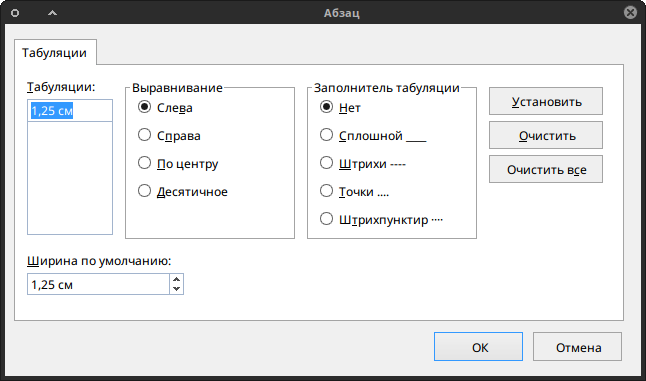
\includegraphics[scale=0.6]{00040.png}
 \item В диалоговом окне \textbf{Табуляции} введите желаемое значение для позиции относительно левой границы страницы, где значение «0» соответствует непосредственно левой границы страницы.
 \item При желании, выберите другое \textbf{Выравнивание} и другой \textbf{Заполнитель} табуляции для шага табуляции (см. ниже).
 \item \textit{Не забудьте} нажать на кнопку \textbf{Установить}.
 \item При необходимости, точно также настройте дополнительные шаги табуляции, и завершите работу в диалоговом окне нажатием кнопки \textbf{OK}.
\end{enumerate}

После настройки шагов табуляции, с помощью клавиши \keys{Tab} их можно вставлять в документ.

\textbf{Внимание}: этот диалог можно также использовать для указания \textbf{Стандартной ширины} для предварительно настроенных шагов табуляции, о которых мы упоминали ранее. Но после установки пользовательских шагов табуляции для конкретного абзаца, предварительно настроенные стандартные шаги игнорируются.

\subsubsection{Выравнивание табуляции}
С помощью команды \textbf{Формат>Табуляции} можно установить не только позицию для нового шага, но также и его выравнивание:

\begin{center}
\begin{tabular}{ | m{4cm} | m{10cm} | }
\hline
 \textbf{Выравнивание} & \textbf{Эффект} \\ 
 \hline
 Слева & Обычный шаг табуляции аналогичный шагу пишущей машинки. Шаг табуляции отмечает место, с которого \textit{начинается} текст.\\
\hline
Справа & Текст после шага табуляции выравнивается по правому краю. Шаг табуляции отмечает место, где текст \textit{заканчивается}.\\
\hline
По центру & Текст, вводимый после шага табуляции, центрируется по позиции табуляции. Шаг табуляции отмечает \textit{середину} вводимого текста.\\
\hline
Десятичное & Для форматирования цифровых столбцов. Цифры располагаются таким образом, чтобы \textit{десятичные разделители} были выравнены по вертикали.\\
\hline
\end{tabular}
\end{center}

\textbf{Совет}: чтобы изменить выравнивание уже существующего шага табуляции, вызовите команду \textbf{Формат>Табуляции}. Выберите один из  настроенных шагов табуляции, измените его выравнивание и нажмите на кнопку \textbf{«Установить»}.

\subsubsection{Заполнитель табуляции}
При желании, пространство шага табуляции можно заполнить следующими символами заполнения:

\begin{center}
\begin{tabular}{ | m{3cm} | m{3cm} | m{7cm} |}
\hline
 Нет &  & Табуляция без заполнения\\ 
 \hline
Сплошной &  & Заполнение сплошным подчеркиванием\\
\hline
Штрихи & \Kutline\Kutline\Kutline\Kutline\Kutline\Kutline & Заполнение штрихами\\
\hline
Точки & \dots\dots\dots\dots\dots\dots\dots & Заполнение точками\\
\hline
Штрихпунктир &      &  Заполнение штрих-пунктиром\\
\hline
\end{tabular}
\end{center}

\textbf{Совет}: чтобы заполнить уже существующую табуляцию, вызовите команду \textbf{Формат>Табуляции}. Выделите один из настроенных шагов табуляции, выберите нужный заполнитель в поле \textbf{Заполнитель табуляции} и нажмите на кнопку \textit{«Установить»}.

\subsubsection{Удаление и перемещение шагов табуляции}
Уж настроенные шаги табуляции можно в любое время изменить. Для этого, выберите абзац, в котором нужно изменить шаги табуляции, и вызовите команду \textbf{Формат>Табуляции}.

Чтобы удалить один из шагов табуляции, выберите его в списке Табуляции и нажмите на кнопку \textbf{Очистить}. Чтобы удалить все шаги табуляции, используйте кнопку \textbf{Очистить все}.

Переместить шаг табуляции на новую позиция с помощью команды \textbf{Формат>Табуляции} невозможно. Можно только удалить шаг табуляции и настроить новый на нужной позиции. Передвинуть шаг табуляции можно с помощью горизонтальной линейки, о чём рассказывается в следующем разделе.

\subsubsection{Использование горизонтальной линейки}
Все шаги табуляции, настроенные для текущего параграфа, показываются на горизонтальной линейке, как можно посмотреть на иллюстрации ниже:

\begin{figure}[ht]

\includegraphics[scale=0.6]{00041.png}
\centering
\caption{Горизонтальная линейка с несколькими табуляциями с левым выравниванием}
\end{figure}

С помощью линейки шаги табуляции можно устанавливать, перемещать и удалять.

Чтобы установить шаги табуляции сделайте следующее:
\begin{enumerate}
 \item Разместите текстовый курсор в нужном абзаце (или выберите несколько абзацев).
 \item Чтобы выбрать нужный тип табуляции , нажмите на один из следующих значков на панели \textbf{Форматирования}:\\
 
\includegraphics[scale=0.6]{00023.png} Выравнивание слева\\
 
\includegraphics[scale=0.6]{00024.png} Выравнивание справа (тест заканчивается на позиции табуляции)\\
 \includegraphics[scale=0.6]{00025.png} Выравнивание по центру (текст центрируется по позиции табуляции)\\
 \includegraphics[scale=0.6]{00026.png} Десятичное (десятичные разделители чисел выравниваются по отметке табуляции)
 
 Также, чтобы изменить тип табуляции, можно нажать на значок непосредственно слева от линейки. Каждое нажатие мышки вызывает следующий доступный тип табуляции.
 \item И наконец, просто нажмите на нужную позицию на линейке, чтобы установить шаги табуляции.
\end{enumerate}

Если позиция шага табуляции пользователя не удовлетворяет, её можно легко изменить, нажав на неё и протащив на новую позицию на линейке.

Чтобы удалить шаг табуляции, стащите отметку вниз, вне области линейки.

\subsection{Маркированные списки}
Списки, в которых каждый пункт списка расположен в отдельном абзаце, и отмечен маркером, гораздо легче читаются, чем списки, разделённые запятыми. Значки, используемые для таких списков, называются \textit{маркерами}.

Создание маркированных списков является легкой задачей для пользователей TextMaker: TextMaker добавляет маркеры к спискам и автоматически их вставляет с помощью нажатия одной клавиши.

 Также можно использовать списки, в которых пункты отмечены цифрой, а не маркером. В этом случае абзацы нумеруются автоматически по порядку, т.е. 1, 2, 3, и т.д.  информацию об этом можно найти в главе «Автоматическая нумерация», которая начинается на стр.175.

\subsubsection{Добавление маркеров}
Чтобы начать маркированный список, сделайте следующее:
\begin{enumerate}
 \item Вызовите команду \textbf{Формат>Маркеры и нумерация}.
 \item Перейдите на вкладку \textbf{Маркеры и простая нумерация}.
 \item В тестовом блоке \textbf{Тип} выберите нужный \textbf{Маркер}.\\
 \includegraphics[scale=0.6]{00042.png}
 \item Выберите нужный тип маркера, нажав на один из маркеров в текстовом блоке \textbf{Маркер}.
 \item Подтвердите выбор с помощью кнопки \textbf{OK}.
 \item Теперь вводите текст. В конце абзаца нажмите клавишу \keys{Enter}, чтобы начать новый абзац. TextMaker автоматически применяет отступ и добавляет маркер.
\end{enumerate}

Конечно, добавить маркер к абзацу можно и после того, как список был напечатан. Для этого выделите текст, вызовите команду, описанную выше, и выберите маркер.

\subsubsection{Удаление маркеров}
Чтобы закончить список или удалить существующие маркеры, сделайте следующее:
\begin{enumerate}
 \item После ввода последнего пункта маркированного списка нажмите клавишу \keys{Enter} чтобы начать новый абзац.\\
 \textit{Или}: выберите абзац, из которого нужно удалить маркеры.
 \item Вызовите команду \textbf{Формат>Маркеры и нумерация}.
 \item Перейдите на на вкладку \textbf{Маркеры и простая нумерация}. 
 \item Выключите маркеры, выбрав параметр \textbf{Нет} в блоке \textbf{Тип}.
 \item Подтвердите нажатием кнопки \textbf{OK}.
\end{enumerate}

\subsubsection{Параметры диалогового окна}
Вкладка \textbf{Маркеры и простая нумерация} диалогового окна \textbf{Формат>Маркеры и нумерация} предоставляет следующие параметры для маркеров:
\begin{itemize}
 \item Тип\\
 Здесь можно указать тип \textbf{Маркер} или тип \textbf{Нумерация}. (Подробности о нумерации см. в разделе «Простая нумерация», который начинается на стр.176).\\
При выборе параметра \textbf{Нет} --- все существующие маркеры или нумерация удаляется.\\
Переделать маркированный список в нумерованный можно в любое время, сменив Тип на Нумерацию. Естественно, можно проделать и обратную операцию.
\item \textbf{По умолчанию} и \textbf{По выбору пользователя}\\
Здесь можно выбрать тип значка маркера. Предварительно настроенные знаки доступны в ряду \textbf{По умолчанию}. Маркеры из ряда \textbf{По выбору пользователя} можно изменить, для создания пользовательского маркера (см. ниже).
\item \textbf{Цвет} (только для маркеров по умолчанию)\\
Цвет для маркера можно выбрать в выпадающем списке Цвет. Кроме цветов из списка, можно применить свой собственный (см. раздел «Свойства документа вкладка Цвета», который начинается на стр.556).
\begin{mdframed}[backgroundcolor=blue!10]
\textbf{Совет:} при выборе цвета \textbf{Автоматически}, TextMaker автоматически будет устанавливать цвет маркера соответственно цвету шрифта, которым набран соответствующий абзац.
\end{mdframed}
\item \textbf{Размер} (только для маркеров по умолчанию)\\
Здесь при необходимости можно изменить размер маркера (пт).
\begin{mdframed}[backgroundcolor=blue!10]
\textbf{Совет:} при выборе параметра \textbf{Автоматически}, TextMaker автоматически будет устанавливать размер маркера соответственно цвету шрифта, которым набран соответствующий абзац.
\end{mdframed}
\item Кнопка \textbf{Символ} (только для маркеров по выбору пользователя)\\
При выборе маркера из пользовательского ряда, два вышеозначенных параметра заменяются кнопкой \textbf{Символ}. Нажмите на эту кнопку, если необходимо изменить формат символа маркера (размер шрифта, цвет, особое выделение и т.д.)
\begin{mdframed}[backgroundcolor=blue!10]
\textbf{Совет:} если формат символа маркера не был изменён, к маркеру будет автоматически применён формат символов, которыми набран соответствующий абзац.
\end{mdframed}
\item Позиция по горизонтали.\\
Определяет сдвиг текста вправо чтобы освободить место для маркера.
\item Позиция по вертикали\\
Определяет вертикальную позицию маркера на строке. Отрицательное значение опускает маркер, положительное --- поднимает.
\item Вкладка \textbf{Нумерованные списки}\\
В этой вкладке располагаются дополнительные возможности для форматирования списков: нумерованные списки. Нумерованные списки можно сохранить и повторно использовать в случае необходимости. Кроме того, у нумерованных списков может быть многоуровневая нумерация (1., 1.1., 1.1.1 и т.п.).\\
Подробности о нумерованных списках можно найти в разделе \textbf{Нумерованные списки}, который начинается на стр.180.
\end{itemize}

\subsubsection{Использование маркеров, настроенных пользователем}
Если имеющиеся значки маркеров в диалоге, описанные выше, не удовлетворяют пользователя, можно выбрать свой значок из множества пользовательских.

Как мы помним, в диалоговом окне этой команды присутствует два ряда значком маркеров: маркеры в ряду \textbf{По умолчанию} нельзя изменить. Напротив, маркеры в ряду \textbf{По выбору пользователя} можно изменять по своему желанию.

Для этого проделайте следующие шаги:
\begin{enumerate}
 \item В пользовательском ряду нажмите на значок который нужно изменить.
 \item Нажмите на кнопку \textbf{Изменить} справа от ряда.
 \item Появится таблица с символами. Сначала установите \textbf{Шрифт}.\\
 {\footnotesize \textit{\textbf{Совет пользователям Windows}: шрифты Symbol и Wingdings содержат множество символов, пригодных для использования в качестве маркеров.}}
 \item Сделайте двойной щелчок по символу, который нужно выбрать.
 \item Выбранный символ появится в ряду пользовательских маркеров. Нажмите на кнопку \textbf{OK} для применения.
\end{enumerate}

\begin{mdframed}[backgroundcolor=blue!10]
\textbf{Внимание:} хотя в диалоговом окне показано только шесть маркеров, пользователь не ограничен только шестью маркерами. Пользовательские маркеры можно переопределить так часто, как это нужно пользователю --- даже в рамках одного документа.
\end{mdframed}

\subsection{Буквица}
Буквицей называется большая декоративная буква в начале абзаца.

TextMaker может создавать такие буквы автоматически, используя первую букву абзаца, и автоматически форматирует последующий текст абзаца так, что он красиво обрамляет эту букву.
\begin{mdframed}[backgroundcolor=blue!10]
\textbf{Внимание:} буквицы можно использовать только в абзацах с выравниванием \textbf{Слева} или \textbf{По ширине страницы}.
\end{mdframed}

Чтобы создать буквицу, выполните следующее:
\begin{enumerate}
 \item Расположите текстовый курсор в том абзаце, в котором нужно создать буквицу.
 \item Вызовите команду \textbf{Формат>Буквица}
 \item В параметрах \textbf{Буквица} выберите желаемый тип.
 \item Выберите нужный \textbf{Размер} шрифта. Если шрифт буквицы должен отличаться от шрифта остального абзаца, нажмите на копку «Шрифт» и укажите нужные параметры шрифта.
 \item Измените \textbf{Поля} для буквицы.
\end{enumerate}

После подтверждения выбранных параметров с помощью кнопки \textbf{OK}, TextMaker отформатирует буквицу для выбранного абзаца. Содержимое абзаца можно будет изменять в обычном режиме.

\subsubsection{Удаление буквицы}
Чтобы удалить буквицу, снова вызовите команду \textbf{Формат>Буквица} и укажите параметр «Нет» в поле \textbf{Буквица}. 

\subsection{Заливка}
С помощью команды \textbf{Формат>Заливка} можно добавить цветную заливку или узор для указанного абзаца в тексте.

\includegraphics[scale=0.6]{00042.png}

Для этого выберите нужный абзац, вызовите команду \textbf{Формат>Заливка} и затем продолжайте следующим образом:
\begin{itemize}
 \item \textbf{Добавление заливки}\\
 В указанный абзац можно добавить цветную заливку из смешанных цветов переднего плана и фона.\\
 Чтобы добавить заливку, выберите Тип «Заливка» и укажите следующие параметры:\\
Сначала выберите цвета \textbf{Переднего плана} и \textbf{Фона} (цвет фона по умолчанию — белый).\\
В разделе Оттенки теперь будут предложено несколько комбинаций из смешанных указанных цветов, нажмите на один из них, для выбора. Или можно ввести точное процентное соотношение каждого цвета в текстовом блоке ниже. Диапазон значений — от 0 (100\% цвет фона) до 100 (100\% цвет переднего плана).
\item \textbf{Добавление узора}\\
Чтобы добавить узор, нажмите на один из них в разделе \textbf{Узоры}.\\
Также для узора можно выбрать различные цвета \textbf{Фона} и \textbf{Переднего плана}.
\item \textbf{Удаление заливки или узора}\\
Чтобы удалить заливку или узор, отметьте пункт \textbf{«Нет»}. 
\end{itemize}

Подтвердите параметры нажатием на кнопку \textbf{OK}.

\subsection{Границы и линии}
Команда \textbf{Формат>Границы} даёт возможность разместить линии границ в абзацах и некоторых объектов. Линии можно добавить слева, справа, сверху и/или снизу абзаца или объекта.

При вызове этой команды появляется следующее диалоговое окно:

\begin{figure}[ht]
\includegraphics[scale=0.6]{00044.png}
\centering
\caption{Диалог для линий границ (здесь: для ячеек таблицы)}
\end{figure}

Аналогичный диалог появляется для всех типов объектов, к которым можно применить границу (например, текстовые рамки или ячейки).

Обычно, работа в таком диалоге происходит следующим образом:
\begin{enumerate}
 \item Сначала указывается, какой именно \textit{тип} границы нам нужен (т.е. выбирается стиль линии, толщина и цвет).
 \item Затем  выбирается, \textit{где} должна применяться указанная линия — с помощью щелчка по соответствующим линиям в диалоге предпросмотра в правой половине диалогового окна (или по кнопкам вокруг него).
\end{enumerate}

\begin{mdframed}[backgroundcolor=blue!10]
\textbf{Внимание пользователи, производящие обновление:} в версиях SoftMaker Office 2012 и более ранних, эти действия должны были производиться в обратном порядке.
\end{mdframed}

Рассмотрим всю процедуру подробно:

Например, пользователю нужно добавить границы для текстового абзаца:
\begin{enumerate}
 \item Разместите текстовый курсор в нужном абзаце (или выберите несколько нужных абзацев).
 \item Вызовите команду \textbf{Формат>Границы}. 
 \item Сначала нужно выбрать какой тип границы нам нужен --- с помощью следующих параметров:\\
\textbf{Стиль} линии (одиночная, двойная или пунктир)\\
\textbf{Толщина} линии\\
\textbf{Цвет} линии
\item Затем нужно выбрать, где должна применяться эта линия (сверху, снизу, слева, справа и т.д.)\\
Для этого в правой части диалогового окна доступен блок предварительного просмотра, окружённый набором кнопок. Используйте его следующим образом:\\
А) При нажатии на одну из линий в области предпросмотра, выбранный тип линии применяется к соответствующей границе.\\
Б) Или можно нажать на кнопки, расположенные сверху и снизу области просмотра. Каждая кнопка представляет один тип границы (указанный символом значка кнопки).\\
В) К кнопкам, расположенным над областью предварительного просмотра, привязаны следующие значения:\\
Кнопка \textbf{Контур} применяет настроенную линию ко всем внешним границам.
Кнопка \textbf{Внутри} применяет эти же настройки ко всем внутренним линиям (например, к ячейкам таблицы).
Кнопка \textbf{Нет} удаляет все линии.
\item Добавьте необходимое количество линий, повторяя шаг 4.\\ 
Конечно, всегда можно изменить параметры линий (шаг 3) перед их добавлением (шаг 4).
\item Закончив, подтвердите настройки с помощью кнопки \textbf{OK}.
\end{enumerate}

Подробности о каждом параметре этого диалога см. ниже.

\subsubsection{Изменение или удаление существующих линий границы}
Стиль, толщину или цвет существующей линии границы можно изменить в любое время, как и удалить линии. Для этого снова вызовите диалог \textbf{Формат>Границы} и выполните следующее:
\begin{itemize}
 \item \textbf{Изменение}: чтобы изменить внешний вид линии сначала необходимо выбрать нужные значения (стиль, толщину, цвет). Затем нажмите на нужную линию в области предварительного просмотра (или на соответствующую кнопку в этой области) чтобы применить эту линию.
 \item \textbf{Удаление}: чтобы удалить линию границы дважды нажмите на её (или на соответствующую кнопку) в области предварительного просмотра. Одно нажатие применяет линию к границе, двойное — удаляет её снова.
\end{itemize}

\textbf{Совет}: кнопка \textbf{Нет}, расположенная над областью просмотра, удаляет все линии сразу.

\subsubsection{Параметры диалога}
Полное описание всех параметров диалогового окна границ и линий:

\begin{itemize}
 \item \textbf{Стиль линии}\\
 Определяет тип создаваемой линии. Можно выбрать между несколькими вариантами одинарной, двойной или пунктирной линии.
 \item \textbf{Толщина}\\
 Определяет толщину линии.
 \item \textbf{Цвет}\\
 Здесь можно изменить цвет линии.\\
 Можно использовать уже существующие цвета, или же собственные цвета (см. раздел Свойства документа, вкладка Цвета», который начинается на стр.556).
 \item \textbf{Поле просмотра}\\
 Область предварительного просмотра располагается в правой части диалога. Оно даёт представление о том, как будут выглядеть линии границ после применения указанных в диалоге параметров.\\
 Кроме того, область просмотра также даёт возможность добавлять и удалять линии следующим образом:\\
 При щелчке по одной из границ, показанных в просмотре, применяется соответствующая линия (с настроенным стилем, толщиной и цветом). При повторном щелчке линия удаляется.\\
 Кроме того, для этой же задачи доступны кнопки слева и под областью просмотра. Каждая кнопка представляет одну границу (что указывается соответствующим значком на кнопке).\\
 Кнопки, расположенные над областью просмотра, представляют собой сочетания команд: \textbf{Нет} --- удаляет все линии сразу, \textbf{Внутри} --- добавляет линии ко всем внешним границам, \textbf{Внутри} --- применяет эти же настройки ко всем внутренним линиям (например, к ячейкам таблицы).
 \item \textbf{Пределы}\\
 Применяются только для текстовых абзацев, определяют, где должны начинаться и заканчиваться линии.\\
 Доступные значения:\\
 \textbf{Поля страницы}: линии идут от левого поля страницы до правого.\\
 \textbf{Отступы параграфа}: линии идут от левого отступа абзаца до правого. Это является значением по умолчанию.\\
 \textbf{Текст}: линии имеют ту же ширину, что и окружаемый ими текст.
 \item Расстояние от текста\\
 Только для текстовых абзацев, определяет расстояние от линии до текста.
\end{itemize}

\subsection{Уровень структуры}
Объёмные документы (например, руководства) обычно организованы и составлены на базе \textit{структуры}.

Для настройки и изменения структуры документа, TextMaker предоставляет \textit{Структурный режим}. Здесь можно присвоить обычный текст заголовкам, повысить или понизить структурный уровень заголовков.

\begin{mdframed}[backgroundcolor=blue!10]
\textbf{Внимание:} как правило, структурный уровень абзаца не меняют вручную с помощью команды \textbf{Формат>Абзац} --- обычной практикой является использование для этого кнопок в Структурном режиме.
\end{mdframed}

В тех редких случаях, когда структурный уровень нужно изменить вручную, вызовите команду \textbf{Формат>Абзац}, переключитесь на вкладку \textbf{Абзац} и укажите нужный уровень с помощью элемента управления \textbf{Уровень структуры}.

Подробности о работе со структурными уровнями можно найти в разделе «Структура», который начинается на стр.408.

\subsection{Принудительная вставка разрывов страниц и столбцов перед абзацем}
TextMaker может всегда вставлять разрыв страницы или столбца перед текущим абзацем. Для этого вызовите команду \textbf{Формат>Абзац}, перейдите на вкладку  \textbf{Направление текста} и активируйте параметр \textbf{Разрыв колонки} или \textbf{Разрыв страницы}.

С этого момента TextMaker всегда будет вставлять разрыв страницы или колонки перед данным абзацем, даже если он будет передвинут на другую позицию в тексте.

\subsection{Контроль абзацев}
Вкладка \textbf{Направление текста} диалога \textbf{Формат>Абзац} также предоставляет возможности для ограничения способов автоматического разделения документа на страницы, для того чтобы обеспечить желаемый внешний вид страниц.

В групповом блоке \textbf{Интервал} для этого существуют следующие возможности:
\begin{itemize}
 \item \textbf{Не отрывать от следующего}\\
 Если этот параметр отмечен, TextMaker не будет вставлять автоматический разрыв страницы, который бы разделил текущий абзац от последующего. Вместо этого TextMaker вставит разрыв перед текущим абзацем.
 
 Если было выбрано несколько абзацев, то не будут разрываться эти абзацы \textit{плюс абзац, который следует за ними}.
 \item \textbf{Не разрывать}\\
 Этот параметр не даёт TextMaker вставлять разрыв страницы посреди абзаца. Вместо этого, TextMaker будет вставлять разрыв перед абзацем, чтобы весь абзац поместился на следующей странице.
 \item \textbf{Запретить висячие строки}\\
 Этот параметр не даёт разрывать абзац так, чтобы в нём появлялись висячие строки. Висячие строки --- это одна строка, отделённая разрывом страницы от других строк абзаца. Это неприятно для глаз и препятствует комфортному прочтению документа.\\
 Если этот параметр включен, то разбиение на страницы выполняется таким образом, чтобы разрыв страницы не оставлял меньше, чем две строки абзаца на странице. Если абзац никак нельзя разбить таким образом, например, если в абзаце всего две строки, то весь абзац будет размещён на следующей странице.
\end{itemize}

\subsection{Неразрывные пробелы}
Существует ещё один способ контроля положения текста на странице:

В некоторых случаях бывает необходимо, чтобы два слова, разделённых пробелом, помещались в одной строке. Но TextMaker об этом не догадывается, и может автоматически разместить эти слова в разных строках. 

Пример: нам необходимо, чтобы все слова в словосочетании «29,800 Руб» находились вместе и не разрывались. Это можно обеспечить, вставив так называемый \textit{неразрывный пробел} или \textit{защищённое пространство} между «29,800» и «Руб». Чтобы вставить такой пробел, нажмите сочетание клавиш \keys{Ctrl}+\keys{Shift}+\textbf{Пробел} вместо простого пробела.

На печати неразрывный пробел выглядит точно так же, как и обычный. Он отличается только программно, чтобы TextMaker размещал целевые слова на одной строке.

\subsection{Подавление нумерации строк}
Параметр \textbf{Подавлять нумерацию строк} вкладки \textbf{Направление текста} диалогового окна \textbf{Формат>Абзац} действует следующим образом:

Во вкладке \textbf{Направление текста} диалогового окна \textbf{Формат>Абзац} можно настроить TextMaker на показ номеров строк в левом поле документа. Для тех абзацев, в которых \textit{не нужно} показывать номера строк, просто отключите параметр \textbf{Подавлять нумерацию строк}.

Подробности про номера строк можно посмотреть в разделе \textbf{Добавление нумерации строк}, стр.190.

\section{Форматирование страниц}
В этой главе освещается всё, что касается форматирования страниц в TextMaker. Сюда входят следующие разделы:
\begin{itemize}
 \item \textbf{Вставка разрывов страниц вручную}\\
 Если пользователю нужно начать новую страницу до того, как текст достигнет конца текущей страницы, всегда можно вставить разрыв страницы вручную. Подробности смотрите в данном разделе.
\item \textbf{Параметры страницы}\\
\item Указать формат страницы для документа можно с помощью команды \textbf{Файл>Параметры страницы}. Здесь можно настроить такие параметры, как размер бумаги, ориентация страницы (книга или альбом) и поля.
\item \textbf{Верхние и нижние колонтитулы}\\
Верхние и нижние \textit{колонтитулы} --- это строки текста, которые повторяются на каждой странице в верхней и в нижней части документа соответственно. В этом разделе описывается, как их создавать и изменять.
\item Верхние и нижние колонтитулы являются частью так называемой \textit{главной страницы}. В главную страницу можно вставить любые типы объектных рамок, например, рамку с водяным знаком. Объекты, добавленные в главную страницу, содержатся на каждой странице документа.
\item \textbf{Разделение документа на главы}\\
Изменение любого из вышеописанных параметров влияет на документ целиком --- если только не разделить документ на \textit{главы}. У каждой главы может быть своё собственное форматирование страницы. Документ нужно разделить на главы в том случае, если, например, нужно изменить нижний и верхний колонтитул или формат бумаги посредине документа. Прочитайте этот раздел, чтобы больше узнать про главы.
\item \textbf{Изменение фона страницы}
\begin{mdframed}[backgroundcolor=pink!50]
\textbf{\textit{FreeOffice}:} команда \textbf{Формат>Фон страницы} отсутствует в \textbf{SoftMaker \textit{FreeOffice}}.
\end{mdframed}
Можно изменить фон страниц документа, например, сделать их цветными. Для этой цели доступно две команды:\\
\textbf{Формат>Фон страницы} и \textbf{Формат>Глава}. В этом разделе вы узнаете, как работать с этими командами, и чем они отличаются.
\end{itemize}

\subsection{Вставка разрывов страниц вручную}
Обычно TextMaker заполняет страницы документа автоматически --- сверху донизу. Когда текст достигает конца страницы, выполняется автоматический разрыв страницы, и текст продолжается на следующей. В случае необходимости начать новую страницу \textit{до} того, как текст дойдёт до конца текущей страницы, всегда можно прибегнуть к \textit{ручному разрыву страницы}.

Если у вас возникла такая необходимость, то для этого нужно разместить текстовый курсор в том месте, где должна начинаться следующая страница, и вызвать команду \textbf{Вставить>Разрыв>Разрыв страницы}. Или можно нажать сочетание клавиш \keys{Ctrl}+\keys{Enter}.

TextMaker вставит принудительный разрыв.

Для удаления такого разрыва нужно разместить текстовый курсор в начале первой строки, непосредственно \textit{следующей за} разрывом, и нажать клавишу \keys{BackSpace}.

\subsection{Разрыв страницы в начале конкретного абзаца}
Принудительный разрыв можно вставлять не только с помощью команды \textbf{Вставить>Разрыв>Разрыв страницы}, но также присвоив абзацу атрибут «всегда начинается с новой страницы».

Для этого нужно разместить текстовый курсор в нужном абзаце, вызвать команду \textbf{Формат>Абзац}, перейти на вкладку \textbf{Направление текста} и отметить параметр \textbf{Разрыв страницы}. TextMaker \textit{всегда} будет вставлять разрыв страницы перед этим абзацем, даже при переносе этого абзаца на другое местоположение в документе.

\subsection{Параметры страницы}
С помощью команды \textbf{Файл>Параметры страницы} можно указать формат страниц в документе. Здесь настраиваются такие параметры, как размер бумаги, ориентация страницы (книга или альбом) и поля.

\begin{figure}[ht]
\includegraphics[scale=0.6]{00045.png}
\centering
\caption{Диалоговое окно команды \textbf{Файл>Параметры страницы}}
\end{figure}

Присутствуют следующие параметры:
\begin{itemize}
 \item \textbf{Ориентация}\\
 Определяет \textbf{ориентацию} документа на отпечатанной странице: \textbf{книжная} или \textbf{альбомная}.
 \item \textbf{Бумага}\\
 Здесь можно указать размер бумаги, под которую форматируется документ. Выпадающий список \textbf{Размер} содержит все размеры, поддерживаемые текущим принтером. Отсутствующий размер можно ввести вручную в полях \textbf{Ширина} и \textbf{Высота}.
 \item \textbf{Поля}\\
 Значения для полей страницы.
 \item \textbf{Переплёт}\\
 Кроме полей страницы, можно также настроить переплёт. Для этого выберите расположение переплёта и введите размер.
 \item \textbf{Подача бумаги}\\
 \textbf{Параметр доступен только в ОС Windows}: при наличии у принтера нескольких лотков для подачи бумаги, здесь можно выбрать, какой из них нужно использовать. Если вы не хотите, чтобы TextMaker как-то влиял на эти параметры, необходимо оставить значение по умолчанию \textbf{Использовать настройки принтера}. С другой стороны, если необходимо напечатать первую страницу на бумаге из лотка 1, а остальные страницы --- из лотка 2, то тогда настраивайте эти параметры соответственно.
 \item Вкладка \textbf{Глава}\\
 В этой вкладке находятся параметры, имеющие отношение к формату главы, который обсуждается в разделе «Деление документа на главы» (который начинается на стр.114).
 \end{itemize}
 
 \begin{mdframed}[backgroundcolor=blue!10]
\textbf{\textit{Внимание}:} изменение этих параметров влияют на \textit{весь} документ, если только не разделить его на \textit{главы}. У каждой главы может быть своё собственное форматирование страницы. Документ нужно разделить на главы в том случае, если, например, необходимо изменить нижний и верхний колонтитул или формат бумаги посредине документа (см. раздел «Деление документа на главы», начинающийся на стр.114).
\end{mdframed}

\subsection{Верхние и нижние колонтитулы}
Верхние и нижние \textit{колонтитулы} --- это строки с текстом, которые печатаются на каждой странице, в верхней и нижней части документа соответственно.

TextMaker располагает верхние колонтитулы на верхних полях страницы, нижние --- на нижних. При изменении полей документа, расположение и размеры колонтитулов настраиваются автоматически.

На следующих страницах вы можете узнать всё, что необходимо знать про колонтитулы.

\subsubsection{Создание и изменение колонтитулов}
Чтобы ввести текст колонтитула, вызовите команду \textbf{Вставить>Колонтитул}. TextMaker разместит текстовый курсор в рамке верхнего колонтитула в верхнем поле документа. Здесь можно ввести и отформатировать текст как обычно.

Рамка верхнего колонтитула обычно состоит из одной строки, тем не менее, по мере ввода текста, или в результате нажатия клавиши \keys{Enter}, она может вырасти за пределы одной строки.

Чтобы переместиться к обычному тексту из рамки колонтитула, просто нажмите мышкой где-нибудь в обычном тексте. Если позже возникнет необходимость редактирования колонтитула, вызовите команду \textbf{Вставить>Перейти к колонтитулу} или нажмите на рамку колонтитула, чтобы вернуться к нему и выполнить редактирование.

\begin{mdframed}[backgroundcolor=blue!10]
\textbf{Внимание:} изменение этих параметров влияют на весь документ, если только не разделить его на \textit{главы}. У каждой главы может быть своё собственное форматирование страницы. Документ нужно разделить на главы в том случае, если, например, необходимо изменить нижний и верхний колонтитул или формат бумаги посредине документа (см. раздел «Деление документа на главы», начинающийся на стр.114).
\end{mdframed}

\paragraph{Совет: использование панели колонтитулов}
TextMaker предоставляет полезный инструмент для редактирования колонтитулов: \textit{панель колонтитулов}.

\begin{figure}[ht]
\includegraphics[scale=0.6]{00046.png}
\centering
\caption{Панель колонтитулов}
\end{figure}

Эта панель появляется автоматически, если расположить текстовый курсор в колонтитуле, если только панель не была отключен. Если панель не показывается, вызовите команду \textbf{Вид>Панели инструментов} и поставьте галочку для «Колонтитулов».

Значки на панели отвечают за следующие функции (слева направо):
\begin{itemize}
 \item Изменить свойства текущего колонтитула (см. раздел «Изменение параметров колонтитулов», который начинается на стр.109)
 \item Изменить формат страницы (вызывает команду \textbf{Файл>параметры страницы})
 \item Вставить верхний колонтитул (или перейти к существующему)
 \item Вставить нижний колонтитул (или перейти к существующему)
 \item Удалить текущий нижний или верхний колонтитул
\item Вставить поле номера страницы
\item Вставить поле количества страниц
\item Вставить другие поля (вызывает команду \textbf{Вставить>Поле})
\item Перейти на предыдущий колонтитул
\item Перейти к следующему колонтитулу
\item Переключиться между верхним и нижним колонтитулом
\item Выйти из колонтитула (переместить текстовый курсор в обычный текст)
\end{itemize}

\begin{mdframed}[backgroundcolor=blue!10]
\textbf{\textit{Совет}:} если направить курсор мыши на один из значков, не нажимая на него, появится текстовое поле с описанием функционала этого значка
\end{mdframed}

\subsubsection{Вставка номеров страниц, даты и т.п.}
Колонтитулы часто содержат номера страниц, дату и т.п. В TextMaker можно вставлять подобную информацию с помощью функционала под названием \textit{поля}.

Для этого переместите текстовый курсор на желаемую позицию в верхнем или нижнем колонтитуле, вызовите команду \textbf{Вставить>Поле} и выберите необходимое поле, например, «Номер страницы» или «Дата печати». Информацию о разных типах полей можно найти в главе «Поля», которая начинается на стр.165.

\textit{\textbf{Совет}}: на \textit{панели колонтитулов} есть кнопки для вставки наиболее часто используемых полей (номер тстраницы, дата и т.д.). См. предыдущий раздел.

\paragraph{Пример: вставка номера страницы в нижний колонтитул}

Чтобы вставить номер страницы в нижний колонтитул, сделайте следующее:
\begin{enumerate}
 \item Нажмите на колонтитул чтобы разместить в нём текстовый курсор.
 \item Вызовите команду \textbf{Вставить>Поле}.
 \item В списке \textbf{Тип поля} выберите пункт «Номер страницы».
 \item Выберите нужный формат нумерации из списка \textbf{Формат}, например, арабский (1, 2, 3, …) или римский (I, II, III …).
 \item Подтвердите с помощью кнопки \textbf{OK}.
\end{enumerate}

TextMaker вставит поле номера страницы в нижнем колонтитуле.

\paragraph{Контроль нумерации страниц}

По умолчанию, первой странице каждого документа присваивается номер «1». тем не менее, при необходимости можно настроить TextMaker начинать с другой цифры.

Для этого вызовите команду \textbf{Формат>Глава}, смените значение параметра \textbf{Номер главы} с \textbf{Приращения} на \textbf{Значение}, и введите нужное начальное число в текстовое поле. Например, «42» --- чтобы присвоить первой странице номер 42.

\subsubsection{Изменение свойств колонтитулов}
Как и все типы рамок, рамки колонтитулов (содержащие колонтитулы), имеют некоторые свойства, которые можно изменить с помощью команды \textbf{Объект>Свойства}. Например, можно изменить высоту или расстояние до текста и полей страницы.

Для этого выполните следующее:

\begin{enumerate}
 \item Нажмите мышкой на рамку колонтитула.\\
 Или вызовите команду \textbf{Вставить>Перейти к верхнему колонтитулу} или \textbf{Вставить>Перейти к нижнему колонтитулу}, что даст аналогичный результат.
 \item Вызовите команду \textbf{Объект>Свойства} чтобы запустить соответствующий диалог.\\ 
 \textbf{Совет}: этот диалог также можно вызвать нажатием на кнопку \includegraphics[scale=0.6]{00047.png} на \textit{панели колонтитулов}.
\end{enumerate}

В этом диалоге можно найти следующие параметры:

\subsubsection{Вкладка «Свойства»}
Во вкладке можно изменить следующие  параметры:
\begin{enumerate}
 \item \textbf{Высота}\\
 Изменяет высоту рамки колонтитула:\\
 \textbf{Не менее}: значение по умолчанию. Высота рамки настраивается автоматически. Чем больше текста вводится, тем больше становится рамка. Текстовое поле справа даёт возможность ввести минимальное значение, если это нужно.\\
 \textbf{Фиксировано}: выбор этого параметра даёт возможность указать точную высоту рамки. Внимание: если этот параметр отмечен, TextMaker будет показывать красную линию на нижней границе рамки колонтитула каждый раз, как рака не будет уменьшаться в указанное значение. В этом случае нужно ввести большее значение для фиксированной высоты или уменьшить количество текста в рамке.
 \begin{mdframed}[backgroundcolor=blue!10]
\textbf{\textit{Внимание}:} \textbf{ширина} колонтитулов настраивается автоматически (чтобы придерживаться левой и правой границы страницы). Тем не менее, чтобы расширить или сузить колонтитул, всегда можно добавить \textit{отступ абзаца}. 
\end{mdframed}
\item \textbf{Расстояние до края}\\
Здесь указывается расстояние между рамкой и нижним/верхним краем страницы.
\item \textbf{Расстояние до текста}\\
Здесь указывается расстояние между рамкой и блоком обычного текста.
\end{enumerate}

\subsubsection{Вкладка «Границы»}
Здесь указываются границы рамки.

Параметры в этой вкладке соответствуют параметрам команды \textbf{Формат>Границы} (раздел «Границы и линии», начинающийся на стр.96).

\subsubsection{Вкладка «Заливка»}
Здесь можно указать фон рамки в виде заливки или узора.

Параметры в этой вкладке соответствуют параметрам команды \textbf{Формат>Заливка} (раздел «Заливка», начинающийся на стр.95).

\subsection{Другие колонтитулы для первой страницы}
Верхние и нижние колонтитулы являются частью так называемой главной страницы (см. также раздел «Главные страницы», начинающийся на стр.112). По умолчанию, содержимое страницы-шаблона повторяется на каждой странице документа.

В случае необходимости можно указать, чтобы для первой страницы документа была использована другая главная страница (включая другие колонтитулы). Это может быть удобно, например, когда первая страница письма должна печататься на предварительном готовом бланке делового письма, а две последующие страницы -- на чистых листах бумаги.

Для этого вызовите команду \textbf{Формат>Глава} и отметьте параметр \textbf{Первая страница отличается}. С этого момента колонтитулы на первой странице можно изменять независимо от колонтитулов остального документа.

\subsection{Разные колонтитулы на левой и правой страницах}
В книгах часто используются разные колонтитулы для левой и правой страниц. Например, на левых страницах руководств номер страницы обычно размещается слева в нижнем колонтитуле, а на правых страницах --- справа.

Чтобы включить разные колонтитулы для разворотов левой и правой страниц, сделайте следующее:

\begin{enumerate}
 \item Вызовите команду \textbf{Формат>Глава}.
 \item Отметьте параметр \textbf{Отличаются левые и правые страницы}.
\end{enumerate}

Теперь стало возможно настроить разные колонтитулы для левых и правых разворотов страниц.

Более детально: при настройке или редактировании колонтитула на любой левой странице документа, колонтитулы для правой страницы будут оставаться не изменёнными. Точно так же изменения колонтитула правой страницы не затронут колонтитул левой.

\subsection{Удаление колонтитулов}
Текст колонтитула можно удалить в любое время, нажав на рамку колонтитула, выделив весь текст и просто удалив его.

При необходимости можно \textit{полностью} удалить рамку колонтитула из документа, хотя обычно этого не требуется. Для этого проделайте следующее:
\begin{enumerate}
 \item Разместите текстовый курсор в рамке колонтитула.
 \item Нажмите на значок \includegraphics[scale=0.6]{00048.png} на панели колонтитулов.\\
 Или можно нажать ПКМ в любой \textit{пустой} области рамки колонтитула и выбрать пункт \textbf{удалить колонтитул} в контекстном меню.
\end{enumerate}

Рамка колонтитула удалена вместе со всем содержимым. В любое время можно настроить новый, с помощью команды \textbf{Вставить>Колонтитул}.

\subsection{Главные страницы}
В этой главе мы уже познакомили вас с колонтитулами, которые нужно ввести только один раз, и они будут присутствовать на \textit{каждой странице} документа. Это очень удобная возможность, но TextMaker приготовил ещё несколько сюрпризов:

Главная страница точно также присутствует на каждой странице документа. Но, как можно судить по названию, она не ограничивается несколькими строчками колонтитула, но может охватывать страницу целиком.

Обратите внимание, что на главной странице разрешены только \textit{рамки} (например, текстовые рамки, рамки рисунков и т.д.).

Если, например, пользователю нужно добавить в деловое письмо «водяной знак», то для этого нужно просто вставить нужную картинку в главную страницу, и затем отметить значение «За текстом» для параметра \textbf{Обтекание текстом}. Водяной знак теперь будет присутствовать на \textit{каждой} странице документа, с текстом поверх него.

\subsubsection{Редактирование главных страниц}
В случае, когда объекты должны присутствовать на \textit{каждой странице} документа или главы, их просто нужно разместить на главной странице. Для этого нужно переключиться в \textit{режим главной страницы} и вставить объекты в страницу.

\begin{mdframed}[backgroundcolor=blue!10]
\textbf{Внимание:} в главную страницу можно вставлять только рамки (текстовые рамки, фреймы рисунков и т.д.) и рисунки. Информацию о работе с этими объектами можно найти в главе «Фреймы и графика», которая начинается на стр.251.
\end{mdframed}

Редактировать главную страницу можно следующим образом:
\begin{enumerate}
 \item Переключитесь в режим главной страницы с помощью команды \textbf{Вид>Главные страницы}.
 \item Внесите необходимые изменения. Например, чтобы вставить изображение, вызовите команду \textbf{Объект>Новая картинка}, для того, чтобы ввести текст, нужно сначала вставить текстовую рамку с помощью команды \textbf{Объект>Новая текстовая рамка}, и т.д.
 \item Закончив редактирование, вызовите команду \textbf{Вид>Стандартный} для выхода из режима главной страницы.
\end{enumerate}

Все вставленные таким образом объекты появятся теперь на \textit{всех} страницах документа.

К сведению: \textit{колонтитулы} также являются частью главной страницы. Не считая того факта, что колонтитулы автоматически размещаются внизу или вверху страницы, в остальном они ведут себя как текстовая рамка, вставленная в главную страницу.

\subsubsection{Несколько главных страниц в одном документе}
По умолчанию, главная страница применяется к документу целиком. Если необходимо использовать разные главные страницы в одном и том же документе, документ необходимо разделить на \textit{главы}, поскольку каждая глава имеет свою главную страницу. Больше информации на эту тему можно найти в разделе «Разделение документа на главы», который начинается на стр.114.

В этом разделе вы узнаете, как настроить главную страницу так, чтобы она применялась только к первой странице документа, а также как создавать разные главные страницы для левых и правых страниц документа.

\begin{mdframed}[backgroundcolor=blue!10]
\textbf{Совет:} в режиме главной страницы тип главной страницы показывается в верхней части каждой главной страницы. Если, например, TextMaker показывает там надпись «Глава 7, правая главная страница», то это соответствует главной странице для всех правых страниц главы 7.
\end{mdframed}

\subsubsection{Блокировка объектов главной страницы в стандартном режиме}
По желанию, объекты, вставленные в главную страницу, могут быть «заблокированы», чтобы предотвратить их случайное перемещение мышью во время редактирования документа в стандартном режиме.  

Чтобы заблокировать такие объекты, вызовите команду \textbf{Файл>Свойства} и перейдите на вкладку \textbf{Вид}. В групповом блоке \textbf{Блокировка} отметьте параметр \textbf{Блокировать объекты на главной странице}.

После блокировки объектов, во время редактирования в стандартном режиме объекты нельзя ни передвинуть ни изменить их размер. Редактировать объекты можно только в режиме главной страницы.

\textbf{\textit{Внимание}}: этот параметр влияет только на текущий документ.

\subsection{Разделение документа на главы}
По умолчанию, параметры форматирования страницы, описанные в этой главе, применяются к документу целиком. То есть все страницы будут иметь одни и те же колонтитулы, формат бумаги и т.д.

\textit{Главы} предоставляют обход для этого ограничения. С помощью команды \textbf{Вставить>Разрыв>Разрыв главы} можно разделить документ на столько глав, сколько это необходимо пользователю. 

Это повлияет на форматирование документа следующим образом:

\begin{itemize}
 \item Для каждой главы можно отдельно настроить \textbf{Формат бумаги}, \textbf{ориентацию} и \textbf{поля}.
 \item Каждая глава может иметь свою отдельную главную страницу и, соответственно, свои собственные \textbf{колонтитулы}.
 \item Для каждой главы можно при необходимости возобновить \textbf{нумерацию страниц}, с любым начальным значением.
 \item При отмеченном параметре \textbf{Отличаются левые и правые страницы} в диалоге форматирования страниц, для левых и правых разворотов страниц можно настроить разные колонтитулы и главные страницы.
 \item Глава может начинаться только на правой или только на левой странице. Если, например, указать только правую страницу, TextMaker автоматически вставит пустую страницу для предотвращения начала главы с левой страницы.
\end{itemize}

Учитывая эти возможности, разделение документа на главы может оказаться удобным в различных ситуациях, а не только при написании объёмной работы, содержащей «главы» в обычном смысле этого слова. Например, это может пригодиться при смене ориентации бумаги с книжной на альбомную посредине документа, для наилучшего размещения широкой таблицы.

Для этого можно вставить разрыв главы, установить ориентацию бумаги в новой главе на альбомную и затем разместить таблицу. Закончив таблицу, вставить после неё ещё один разрыв главы, снова настроить ориентацию на книжную, для продолжения ввода текста.

Подробности о работе с главами можно найти на дальнейших страницах.

\subsubsection{Вставка и удаление глав}
Чтобы начать новую главу, просто вставьте в текст \textbf{разрыв главу}:
\begin{enumerate}
 \item Переместите текстовый курсор на местоположение, где должна начинаться новая глава.
 \item Вызовите команду \textbf{Вставить>Разрыв>Разрыв главы}.\\
 \end{enumerate}
 
 TextMaker вставит разрыв главы.
 
 \begin{mdframed}[backgroundcolor=blue!10]
\textbf{Внимание:} TextMaker всегда выполняет разрыв страницы в начале новой главы.
\end{mdframed}

\textbf{\textit{Совет}}: глава, в которой в данный момент расположен текстовый курсор, показана в поле «Глава» в строке состояния в нижней части окна TextMaker.

\subsubsection{Удаление разрыва главы}
Удалить разрыв главы можно, расположив текстовый курсор в начале абзаца, идущего сразу после разрыва, и нажав затем клавишу \keys{BackSpace}. Глава, расположенная \textit{перед} разрывом будет включена в главу \textit{после} разрыва, и к ней будет применено форматирование этой главы.

\subsection{Главы и форматирование страниц}
\begin{mdframed}[backgroundcolor=blue!10]
\textbf{Внимание:} для каждой главы документа может применяться разный формат страниц.
\end{mdframed}

Напомним, что формат страницы включает в себя:
\begin{itemize}
 \item Формат бумаги, ориентацию и поля
 \item Колонтитулы и главные страницы
 \item Нумерацию страниц
\end{itemize}

При создании нового документа, он изначально состоит из \textit{одной} главы. Соответственно, когда изменяется что-то, имеющее отношение к форматированию страниц, это изменение влияет на документ в целом.

Если разделить документ на главы с помощью команды \textbf{Вставка>Разрыв>Разрыв главы}, то сначала к каждой главе применяется изначальный формат страниц документа. Общее правило таково:

\begin{mdframed}[backgroundcolor=blue!10]
\textbf{Внимание:} при вставке разрыва главы, создаваемая новая глава имеет текущее форматирование страницы и шаблон главной страницы. Но после последующего изменения формата страницы и разметки главной страницы новой главы, эти изменения применяются только для этой созданной главы.
\end{mdframed}

После разделения документа на главы, для каждой главы можно отдельно настроить разные колонтитулы, настроить различный формат бумаги и т.д.

\subsubsection{Форматирование глав}
\textit{Форматирование глав} выходит за рамки \textit{форматирования страниц}, которые можно применять к главам в последовательном режиме, и включает в себя форматирование, относящееся непосредственно к главам как таковым.

Чтобы изменить \textit{формат страницы} главы, используются команды, описанные в главе «Форматирование страниц», начинающейся на стр.103.

Чтобы изменить \textit{формат главы} для главы, выполните следующее:
\begin{enumerate}
 \item Расположите текстовый курсор где-нибудь внутри нужной главы, или выделите несколько глав, чтобы изменить формат для них одновременно. Выделение может начинаться в любом абзаце первой нужной главы и заканчиваться в любом абзаце последней нужной главы.
 \item Вызовите команду \textbf{Формат>Глава}.\\
 \includegraphics[scale=0.6]{00049.png}
 \item Внесите необходимые изменения и подтвердите их с помощью кнопки OK.
\end{enumerate}

Диалоговое окно этой команды предоставляет следующие параметры:
\begin{itemize}
 \item \textbf{Главные страницы}\\
 Здесь присутствуют параметры, имеющие отношение к главным страницам главы (см. также раздел «Главные страницы», начинающийся на стр.112).
 
 \textbf{Первая страница отличается}: если этот параметр отмечен, первая страница главы использует другую главную страницу. Это удобно, если, например, колонтитул первой страницы документа (или главы), должен отличаться от других.
 
 \textbf{Отличаются левые и правые страницы}: удобно для двусторонней печати (книги, например). Если этот параметр отмечен, для разворотов левых и правых страниц настраиваются разные главные страницы (и соответственно, и разные колонтитулы).\\
 \begin{mdframed}[backgroundcolor=blue!10]
\textbf{\textit{Подсказка}:} в режиме главной страницы тип главной страницы показывается в верхней части каждой главной страницы. Если, например, TextMaker показывает там надпись «Глава 7, правая главная страница», то это соответствует главной странице для всех правых страниц главы 7.
\end{mdframed}

\textbf{Границы и заливка главной страницы}: дайте возможность изменить границу и заливку главной страницы (и, соответственно, всех страниц документа в этой главе). При нажатии на кнопку \textbf{Изменить} появляется всплывающее меню, в котором можно выбрать, какой тип главной страницы нужно изменить. Далее показывается обычный диалог для границ, линий и заливки. Также см. раздел «Изменение фона страниц» (стр.119).
\item \textbf{Глава начинается с}\\
При вставке пользователем разрыва главы, TextMaker добавляет разрыв страницы. Соответственно, новая глава всегда начинается на новой странице.

При смене значения параметра \textbf{Глава начинается с} с \textbf{Любой страницы}, например, на \textbf{Правую страницу}, TextMaker следит за тем, чтобы глава всегда начиналась с правой страницы, в случае необходимости автоматически добавляя пустую страницу в конце предыдущей главы.\\
Как пример можно привести общее правило, что главы в печатной книге начинаются на правой странице. Это даёт читателю возможность быстро пролистать книгу в поисках интересующей главы.
\item \textbf{Номер главы}\\
TextMaker автоматически нумерует главы приращением. Номер текущей главы всегда можно увидеть в строке состояния.

При смене значения параметра \textbf{Номер главы} с \textbf{Приращения} (по умолчанию) на \textbf{Значение}, пользовтаель может сам указать номер главы, введя его в текстовое поле. Например, если ввести значение «5» для третьей главы, то главы будут в таком цифровом порядке: 1,2,5,6,7 и т.д.\\
\textbf{\textit{Посказка}}: номер главы всегда можно вставить в текст с помощью команды \textbf{Вставить>Поле}.
\item \textbf{Выравнивание по вертикали}\\
Здесь можно изменить вертикальное выравнивание основного текста на странице.\\
Если,  например, было выбрано значение \textbf{По центру}, текст будет выравнен вертикально по центру страницы. При выборе значения \textbf{По ширине}, абзацы равномерно размещаются таким образом, что  текст начинается сразу под верхним полем страницы, а заканчивается сразу над нижним.
\item \textbf{Номер страницы}\\
Автоматическую нумерацию страниц также можно изменять. Чтобы изменить нумерацию страниц, измените значение параметра \textbf{Номер страницы} с \textbf{Приращения} на \textbf{Значение} и введите желаемое число для первой страницы главы в расположенном здесь же текстовом поле.\\
Если, например, ввести значение «42», то первой страницей главы будет страница 42, второй --- 43 и так далее.\\
Дополнительные сведения об использовании номеров страниц можно найти в разделе «Вставка номеров страниц, даты и т.д.», начинающемся на стр.108.
\item Вкладка \textbf{Формат страницы}\\
В другой вкладке этого диалогового окна можно изменить формат страницы (размер бумаги, ориентация, поля и так далее). Подробную информацию о каждом параметре можно найти в разделе «Параметры страницы», начинающемся на стр.104.\\
Не забывайте, что для каждой отдельной главы можно указывать различный формат страниц. Поэтому, если документ разделён на главы, а вам нужно изменить формат страниц \textit{всего} документа, то сначала нужно выделить весь документ целиком.
\end{itemize}

\subsubsection{Перемещение между главами}
Переместиться в нужную главу можно с помощью команды \textbf{Правка>Перейти к}. Для этого вызовите команду, выберите параметр \textbf{Глава} в списке \textbf{Перейти к} и затем выберите нужную главу.

\subsection{Изменение фона главы}
Как уже упоминалось в разделе «Форматирование глав», изменить фон страниц документа можно с помощью команды \textbf{Формат>Глава}. Таким образом, например, можно добавить цветной фон страницам.

Есть ещё одна команда с аналогичным функционалом, но предлагающая больше параметров для выбора: команда \textbf{Формат>Фон страницы}.
\begin{mdframed}[backgroundcolor=pink!50]
\textbf{\textit{FreeOffice}:} команда \textbf{Формат>Фон страницы} отсутствует в \textbf{SoftMaker} \textbf{\textit{FreeOffice}}.
\end{mdframed}

В этом разделе мы расскажем, как работают эти две команды, и чем они отличаются.

\subsubsection{\textbf{Формат>Фон страницы}}
Команду \textbf{Формат>Фон страницы} можно использовать для смены фона страниц \textit{всего} документа.

Выполните следующее:
\begin{enumerate}
 \item Вызовите команду \textbf{Формат>Фон страницы}.
 \item В списке \textbf{Тип} заполнения выберите тип заливки для фона. Можно выбрать сплошной цвет, узор, рисунок (плиткой) или различные типы цветных градиентов.
 \item Внесите необходимые изменения и нажмите на кнопку OK.
\end{enumerate}

Подробности об этом диалоге см. в разделе «Свойства объектов, вкладка Заливка» (стр.267). Этот раздел описывает практически идентичный диалог заливки для объектов.

\textbf{Печать}: обратите внимание, что такой тип фона страницы показывается только на экране, и \textit{не выводится на печать}. Тем не менее, сущетвует параметр, позволяющий изменить это поведение. При активации параметра \textbf{Печатать фон страницы} во вкладке \textbf{Вид} диалога \textbf{Файл>Свойства}, фон страницы также будет присутствовать в печатном экземпляре документа.

\subsubsection{\textbf{Формат>Глава}}
Команда \textbf{Формат>Глава} работает немного по-другому.

Эту команду можно использовать для изменения фона страницы для текущей \textit{главы} (более конкретно, её главной страницы).

Выполните следующее:
\begin{enumerate}
 \item Если документ был разделён на несколько глав, расположите текстовый курсор в нужной главе.
 \item Вызовите команду \textbf{Формат>Глава}.
 \item В блоке \textbf{Границы и заполнение главных страниц} нажмите на кнопку \textbf{Изменить} и выберите, какой тип главной страницы нужно изменить.
 \item Перейдите на вкладку \textbf{Заливка}.
 \item Выберите нужный \textbf{Тип} заливки. Здесь доступны только цветовые заливки и узоры.
 \item Внесите необходимые изменения и нажмите на кнопку OK.
\end{enumerate}

Подробности об этом диалоге см. в разделе «Заливка» (стр.95). В этом разделе описывается идентичный диалог «Заливка» для текстовых абзацев.

Обратите внимание, что если документ разделён на несколько глав, изменения, внесённые с помощью этой команды, влияют только на текущую главу (см. также раздел «Разделение документа на главы», начинающийся на стр.114).

\textbf{Печать}: этот тип заливки \textit{всегда} выводится на печать. Параметр документа \textbf{Печатать фон страницы}, упомянутый выше, здесь не влияет.

\section{Стили}
\textit{Стиль} --- это удобный помощник продвинутых пользователей текстовых редакторов.

Если пользователю часто приходится прибегать к конкретному формату символов или абзацев, будет более выгодно создать на его основе стиль. После этого такой стиль применяется к любому необходимому фрагменту текста, с параметрами, указанными при создании стиля.

\begin{mdframed}[backgroundcolor=blue!10]
\textbf{\textit{Кроме того}:} использование стилей не только экономит время при частом использовании одного и того же форматирования, но также обеспечивает унифицированность формата документа, поскольку при изменении параметров стиля, формат \textit{всех} фрагментов текста, к которым был применён этот стиль, изменяется соответственно.
\end{mdframed}

Фактически, стили работают таким образом: пользователь настраивает стиль абзаца под названием «Заголовки», с крупным полужирным шрифтом, с выравниванию по центру и тому подобное. После этого, всегда, когда пользователю нужно превратить абзац в заголовок, всё, что для этого нужно сделать --- это применить созданный стиль.

Для каждого документа можно создать разные стили --- все эти стили сохраняются в документе.

В этой главе вы найдёте подробное описание использования стилей. Рассматриваются следующие темы:
\begin{enumerate}
 \item \textbf{Стили символов}\\
 В стиле \textit{символов} можно сохранить часто используемый формат \textbf{символа} (гарнитура, размер, выделение и т.п.) и повторно применять его к любым нужным символам.\\
Для этого используйте команду \textbf{Формат>Стиль символов}.
\item \textbf{Стили абзаца}\\
В стиле \textbf{абзаца} можно сохранить часто используемый формат \textbf{абзаца} (отступы, шаги табуляции, выравнивание и т.п.) и повторно применять его к любым нужным абзацам.
Для этого используйте команду \textbf{Формат>Стиль абзаца}.
\item \textbf{Управление стилями}\\
\begin{mdframed}[backgroundcolor=pink!50]
\textbf{\textit{FreeOffice}:} этот функционал отсутствует в \textbf{SoftMaker \textit{FreeOffice}}.
\end{mdframed}
Встроенный \textit{менеджер стилей} TextMaker даёт возможность управлять стилями в документах. Можно, например, скопировать стиль из одного документа в другой.
Для этого используйте команду \textbf{Формат>Управление стилями}.
\item \textbf{Шаблоны документов}\\
Часто используемые стили можно сохранять в \textit{шаблоне документа}.\\
Каждый раз при создании документа TextMaker предлагает выбрать шаблон, на основе которого будет создан документ. Все стили, хранящиеся в шаблоне, будут также доступны в новом документе.
\end{enumerate}

Подробности смотрите далее.

\subsection{Стили символов}
В стиле \textit{символов} можно сохранить часто используемый формат \textbf{символа} (гарнитура, размер, выделение и т.п.) и повторно применять его к любым нужным символам.

Если, например, некоторые раздела документа-контракта должны быть форматированы специальной гарнитурой меньшего размера, создайте соответствующий стиль символов -- назовём его «Тонкая печать» --- и примените к нужным разделам документа.

\textbf{\textit{Внимание:}} различия между стилями символов и стилями абзацев (см. раздел «Стили абзаца», начинающийся на стр.132) в том, что стили символов содержат только сохранённые форматы символов, в то время как стили абзацев сохраняют и формат \textit{символов} и формат \textit{абзацев} (отступы, шаги табуляции, выравнивание и т.п.).

Соответственно, стили символов применяются к отдельным символам, а стили абзацев применяются только к целым абзацам.

На нижеследующих страницах вы найдёте подробную информацию о работе со стилями символов. Рассматриваются следующие темы:
\begin{itemize}
 \item \textbf{Создание стилей символов}
 \item \textbf{Применение стилей символов}
 \item \textbf{Изменение стилей символов}
 \item \textbf{Область действия стилей символов}
 \item \textbf{Стиль символов «Обычный»}
 \item \textbf{Создание связанных стилей символов}
 \item \textbf{Стили символов и боковая панель}
\end{itemize}

\subsubsection{Создание стилей символов}
Чтобы создать стиль символов, сделайте следующее:
\begin{enumerate}
 \item Вызовите команду \textbf{Формат>Стиль символа}\\
 \includegraphics[scale=0.6]{00050.png}
 \item Нажмите на кнопку \textbf{Новый}.
 \item Дайте своему стилю любое название и нажмите на кнопку \textbf{OK}.
 \item Появится диалоговое окно, очень похожее на диалоговое окно \textbf{Формат>Символ}. Здесь можно указать нужные параметры формата (см. раздел «Форматирование символов», начинающийся на стр.67).
 \item При частом применение стиля, ему можно назначить сочетание клавиш (см. ниже).
 \item Сделав необходимые изменения параметров, нажмите на кнопку OK чтобы создать стиль.
 \item Выйдите из диалога, нажав на кнопку \textbf{Закрыть}.
\end{enumerate}

Стиль создан и готов к использованию. Узнать, как с ним работать, можно в разделе «Применение стилей символов».

\paragraph{Создание стилей символа на основе существующего текста}

Как вариант, можно сначала отформатировать текст, а затем создать стиль символа с этими параметрами форматирования. Для этого вместо кнопки \textbf{Новый} используйте кнопку \textbf{Новый из текста}.

Этот способ удобен в случае «ручного» форматирования текста и получения на его основе стиля с точно таким форматированием.

Выполните следующее:
\begin{enumerate}
 \item Установите формат символа (гарнитура, размер шрифта и т.д.) любого фрагмента текста.
 \item Разместите текстовый курсор внутри этого текста (или выделите этот текст).
 \item Как описано выше,  используйте команду \textbf{Формат>Стиль символа} для создания нового стиля символа. Но в данном случае нужно использовать кнопку \textbf{Новый из текста} вместо кнопки \textbf{Новый}.
 \end{enumerate}

Созданный таким способом стиль символа ведёт себя точно также, как и любой другой стиль символа. Его отличие только в том, что он основан на формате символов выбранного текста. (И конечно, пользователь в любое время может изменить параметры форматирования в этом стиле, вне зависимости от текста.)

\paragraph{Использование горячих клавиш}

В случае когда часто приходится применять стиль, ему можно назначить сочетание клавиш. В этом случае стиль можно применять очень быстро, одним нажатием клавиш.

Чтобы присвоить сочетание клавиш стилю, в диалоге редактирования стиля перейдите во вкладку \textbf{Стиль}. Расположите курсор в окошке \textbf{Горячая клавиша} и нажмите желаемое сочетание клавиш.

\begin{mdframed}[backgroundcolor=blue!10]
\textbf{\textit{Внимание}:} в случае, если эта комбинация клавиш уже \textit{используется}, то её текущее значение будет показано под текстовым окошком \textbf{Горячая клавиша}:

\includegraphics[scale=0.4]{00051.png}

В этом случае нажмите клавишу \keys{BackSpace} для удаления этой комбинации клавиш и ввода другой. В противном случае будет перезаписано уже присвоенное сочетание клавиш для другого стиля или даже команды TextMaker.
\end{mdframed}

Мы рекомендуем использовать сочетание клавиш с \keys{Ctrl} \textit{и} \keys{Shift}, поскольку, как правило, они по умолчанию не присвоены.

\subsubsection{Применение стилей символов}
Чтобы применить стиль символа, выполните следующее:
\begin{enumerate}
 \item Выделите фрагмент текста, к которому нужно применить стиль.
 \item Вызовите команду \textbf{Формат>Стиль символа}.
 \item Выберите нужный стиль.
 \begin{mdframed}[backgroundcolor=blue!10]
\textbf{\textit{Подсказка}:} предварительный просмотр выбранного стиля располагается в правой части диалогового окна. Предпросмотр можно в любое время включить или выключить с помощью кнопок \textbf{>>}и \textbf{<<}.
\end{mdframed}
\item Нажмите на кнопку \textbf{Применить}.
\end{enumerate}

Формат выбранного текста изменится в соответствии с параметрами стиля символа.

\begin{mdframed}[backgroundcolor=blue!10]
\textbf{\textit{Подсказка 1}:} Стили символов можно также выбрать из списке шрифтов на панели Форматирования.
\newline
\newline
\textbf{\textit{Подсказка 2}:} в случае, если стилю присвоено сочетание клавиш, стиль можно применить ещё быстрее. Выделите символ, к которому нужно применить стиль, и нажмите сочетание клавиш.
\newline
\newline
\textbf{\textit{Подсказка 3}:} кроме того, для применения стилей (а также и для их редактирования) можно использовать боковую панель, см. раздел «Стили символов и боковая панель», стр.131).
\end{mdframed}

Чтобы удалить стиль, примените к тексту стиль символов «Обычный». Не забывайте, что тексту, к которому был применён стиль, всегда можно добавить дополнительное форматирование с помощью команды \textbf{Формат>Шрифт}.

\subsubsection{Изменение стилей символов}
Далее подразумевается, что стили символов можно изменять в любое время по желанию.

\begin{mdframed}[backgroundcolor=blue!10]
\textbf{\textit{Важно}:} при изменении стиля символа, форматирование \textit{всех} фрагментов текста, к которым был ранее применён этот стиль, изменяется соответственно. Тем не менее, это автоматическое переформатирование ограничено для тех фрагментов текста, в которых также применялось ручное форматирование символов (см. следующий раздел).
\end{mdframed}
Чтобы редактировать стиль символа, выполните следующее:
\begin{enumerate}
 \item Вызовите команду \textbf{Формат>Стиль символа}.
 \item Выберите из списка стиль, который нужно изменить.
 \item Нажмите на кнопку \textbf{Изменить}.
 \item Внесите нужные изменение в параметры стиля.
 \item Нажмите на кнопку \textbf{OK}.
 \item Закройте диалог нажатием на кнопку \textbf{Закрыть}.
\end{enumerate}

Стиль изменён.

\paragraph{Выбор стилей, которые должны показываться в списке}

По умолчанию, в диалоге, описанном выше, список стилей содержит использованные стили, или стили, изменённые пользователем. Если необходимо просмотреть \textit{все} доступные стили, выберите в параметре \textbf{Показать} значение \textbf{Все стили}. Тогда будут также показаны предварительно настроенные стили.

\paragraph{Изменение стиля для совпадения с текущим текстом}

Кнопку \textbf{Новый из текста} можно использовать для приведения стиля в соответствие с выделенным текстом. В итоге стиль получит параметры форматирования этого текста.

Продолжайте таким образом:
\begin{enumerate}
 \item Настройте формат символа (гарнитура, размер шрифта и т.д.) любого фрагмента текста.
 \item разместите текстовый курсор внутри этого текста (или выделите этот фрагмент).
 \item Вызовите команду \textbf{Формат>Стиль символа}.
 \item Выберите в списке стиль, который нужно  изменить.
 \item Нажмите на кнопку \textbf{Обновить из текста}.
\end{enumerate}

К стилю будут применены параметры форматирования указанного текста. (Конечно, пользователь в любое время может изменить параметры форматирования в этом стиле, вне зависимости от текста.)

\paragraph{Удаление или переименование стиля}

Чтобы удалить стиль в текущем документе, выберите его в диалоге и затем нажмите на кнопку \textbf{Удалить}. Чтобы дать стилю новое название, нажмите на кнопку \textbf{Переименовать} и введите новое имя.

Внимание: для встроенных стилей кнопка \textbf{Удалить} недоступна.

Чтобы удалить или  переименовать стиль в \textit{шаблоне документа} откройте шаблон, внесите изменения и сохраните шаблон.

\subsubsection{Область действия стилей символов}
Что делать, если пользователь изменил стиль символа, но формат некоторых фрагментов текста, к которым был применён ранее этот стиль, не изменился? Это происходит потому, что эти фрагменты текста были повторно отформатированы вручную. Пример:

Предположим, что мы настроили стиль, в котором используется шрифт Arial, и применили его. Если затем сменить шрифт в стиле на Times New Roman, то все фрагменты, форматированные в этом стиле, изменятся соответствующим образом.

\textbf{\textit{Но}}: если для одного из этих текстовых фрагментов шрифт был изменён с помощью команды \textbf{Формат>Шрифт} или с помощью панели Форматирования, то все последующие изменения \textit{стиля} этого фрагмента \textit{не будут применяться} к этому фрагменту текста. То есть ручное форматирование имеет приоритет над стилями.

Если пользователь хочет «освободить» такой фрагмент текста от ручного форматирования, вызовите команду \textbf{Формат>Стандартный}. Тогда для этого фрагмента текста будет восстановлено форматирование, указанное в применённом стиле.

\subsubsection{Стиль символов «Обычный»}
Стиль символов «Обычный» по умолчанию присутствует в каждом документе и имеет особое значение. Он является стандартным текстовым стилем. Если начать вводить текст в новом документе, тексту автоматически присваивается стиль «Обычный», до того момента, когда (и если) будет выбран другой стиль, который будет применяться, начиная от текущей позиции.

Если изменить этот стиль, например, указав новую гарнитуру, то новая гарнитура применится ко всему существующему тексту (если только тексту не была присвоена новая гарнитура с помощью команды \textbf{Формат>Шрифт}.) Более того, гарнитура поменяется в тексте, который будет вводиться после этого, т.к.  изменяя таким образом образом стиль «Обычный», мы изменяем шрифт по умолчанию.

\subsubsection{Создание связанных стилей символов}
Создаваемые стили символов всегда базируются на стиле символов «Обычный», как мы говорили выше. Соответственно, при изменении стиля «Обычный», например, выбрав другую гарнитуру для него, все стили символов, созданные на его основе , также изменятся (кроме тех стилей, где гарнитура была указана специально).

\begin{mdframed}[backgroundcolor=blue!10]
\textbf{\textit{Поэтому}:} по умолчанию, все стили символов связаны со стилем «Обычный». тем не менее, при создании нового стиля можно указать другой базовый стиль в параметре \textbf{На базе}.
\end{mdframed}

Чтобы создать новый стиль на базе \textit{другого} стиля, чем «Обычный», выполните следующее:
\begin{enumerate}
 \item Вызовите команду \textbf{Формат>Стиль символа}.
 \item Нажмите на кнопку \textbf{Новый}.
 \item Укажите название для нового стиля.
\item Перейдите на вкладку \textbf{Стиль}.
\item \textit{Теперь внимание:} в блоке \textbf{На базе} выберите стиль, к которому будет привязан новый стиль.
\item Теперь можно изменять параметры форматирования и так далее.
\end{enumerate}

\textbf{Практический пример}:

Предположим, что для заголовков нашей докторской диссертации нам нужно использовать полужирный шрифт с чёткими и строгими очертаниями. Но нам также нужно. чтобы заголовки были разных размеров, отражающие структуру документов.

Для этого нам нужно выполнить следующее:
\begin{enumerate}
 \item Сначала создадим стиль символов с названием «Заголовки1», для заголовков самого высокого уровня. Здесь мы выбираем конкретную, нужную нам  гарнитуру, указываем размер в 24пт и включаем полужирный формат.
 \item Далее добавим стиль с названием «Заголовки2». В поле \textbf{На базе} выбираем наш стиль «Заголовки1» и указываем размер в 18пт.
 \item Затем создадим стиль символов с названием «Заголовки3», на основе стиля «Заголовки2», с размером в 14пт, и так далее.
\end{enumerate}

Польза: если позже пользователю покажется, что для заголовков подходит другой шрифт, то изменить \textit{все} заголовки со стилями от «Заголовки1» до «Заголовки3» можно всего-навсего изменив параметр шрифта для стиля символов «Заголовки1». А если бы мы создали наши стили на базе стиля «Обычный», то пришлось бы изменять шрифт для каждого стиля отдельно.

\textbf{Относительные размеры шрифтов}
При создании одного стиля на базе другого, в случае необходимости можно указать размер шрифта в \textit{относительной} манере. Например, можно указать, что размер шрифта для стиля X должен всегда составлять 80\% от размера шрифта для стиля Y.

Это можно сделать следующим образом:
\begin{enumerate}
 \item Вызовите команду \textbf{Формат>Стиль символа}.
 \item Выберите стиль и нажмите \textbf{Изменить}.
 \item Переключитесь на вкладку \textbf{Стиль}.
 \item Активируйте параметр \textbf{Масштаб}.
 \item Введите желаемую переменную в виде процента --- например, 80.
 \item Подтвердите с помощью кнопки \textbf{OK}.
\end{enumerate}

Размер шрифта для стиля, указанный таким образом, всегда будет составлять 80\% от размера шрифта, указанного для стиля, на базе которого создан новый стиль.

\subsubsection{Стили символов и боковая панель}
На предыдущих страницах мы научились создавать, применять и изменять стили символов. Эти же операции можно выполнять с помощью другого очень удобного инструмента TextMaker: \textit{боковой панели}.

Боковая панель, помимо всего прочего, может показать список всех доступных стилей символов. Чтобы применить стиль к конкретному тексту, просто выделите текст и сделайте двойной щелчок по нужному стилю на боковой панели.

Кроме этого, боковую панель можно использовать для редактирования и управления стилями. Для этого нужно включить боковую панель и активировать функцию \textit{стили символов}. Это можно сделать следующим образом:

\begin{enumerate}
 \item Если боковая панель не показывается, включите её, вызвав команду \textbf{Вид>Боковая панель>Показать справа}.
 \item На маленькой панели инструментов в верхней части боковой панели нажмите на значок \includegraphics[scale=0.6]{00052.png}. Боковая панель переключится на функционал \textit{стилей символов}. 
\end{enumerate}

На боковой панели теперь показываются все стили символов, доступные в документе, что даёт возможность выполнить следующие действия:

\begin{enumerate}
 \item \textbf{Применение стиля символов}\\
 Сначала выберите символы, которые нужно форматировать, затем сделайте двойной щелчок по нужному стилю на боковой панели.\\
 (Или одним нажатием выберите стиль и затем нажмите на кнопку \textbf{Применить} в нижней части боковой панели.)
 \item \textbf{Изменение стиля символа}\\
 Одним нажатием выберите нужный стиль на боковой панели. Затем нажмите на кнопку \textbf{Правка} в нижней части боковой панели.
 \item \textbf{Управление стилями символов}\\
 Одним нажатием выберите нужный стиль на боковой панели. Затем нажмите на кнопку \textbf{Упорядочить} в нижней части боковой панели.
 Будет показано мини-меню с командами для управления стилями, с помощью которого можно создавать, удалять и переименовывать стили. Подробности о каждой из этих команд можно найти в разделе «Стили символов» (нач. на стр.124).\\
 Подсказка: это меню можно открыть быстрее, сделав щелчок ПКМ по стилю на боковой панели.
 \item \textbf{Создание нового стиля символов}\\
 Сделайте щелчок ПКМ по стилю на боковой панели, на базе которого будет создан новый стиль. Будет показано упомянутое выше мини-меню, в котором нужно выбрать команду \textbf{Новый}.
\end{enumerate}

\subsection{Стили абзаца}
Часто используемый формат абзаца (отступы, шаги табуляции, выравнивание и т.п.) можно сохранить в \textit{стиле абзаца} и применять его повторно к нужным абзацам.

Если, например, заголовки документа должны быть выполнены крупным полужирным шрифтом и выравнены по центру, просто создайте стиль абзаца под названием «Заголовок» и примените его к нужным абзацам.

\textbf{\textit{Внимание}}: различие между стилями символов (раздел «Стили символов», нач. на стр.124) и стилями абзацев заключается в том, что стили символов содержат только сохранённый формат символов (гарнитура, стиль текста и т.д.), а стили абзаца содержат как форматирование \textit{символов}, так и форматирование \textit{абзацев}.

Кроме того, стили символов применяются к отдельным символам, а стили абзацев применяются только к абзацам целиком.

Ниже можно найти подробную информацию о работе со стилями абзацев. Рассматриваются следующие темы:
\begin{itemize}
 \item Создание стилей абзацев
 \item Применение стилей абзацев
 \item Изменение стилей абзацев
 \item Область действия стилей абзацев
 \item Стиль абзацев «Обычный»
 \item Создание связанных стилей абзацев
 \item Стили абзацев и боковая панель
\end{itemize}

\subsubsection{Создание стилей абзацев}
Чтобы создать новый стиль абзаца, выполните следующее:
\begin{enumerate}
 \item Вызовите команду \textbf{Формат>Стиль абзаца}.\\
 \includegraphics[scale=0.6]{00053.png}
 \item Нажмите на кнопку \textbf{Новый}.
 \item Дайте название стилю.
 \item Будет показано диалоговое окно, очень похожее на диалоговое окно \textbf{Формат>Абзац}. Здесь можно указать нужное форматирование абзаца (см. раздел «Форматирование абзаца», нач. на стр.79).
 \item Совет: если стиль абзаца применяется довольно часто, ему можно присвоить сочетание клавиш (см. ниже).
 \item После внесения нужных изменений, нажмите на кнопку OK для создания стиля.
 \item Выйдите из диалога, нажав на кнопку \textbf{Закрыть}.
\end{enumerate}

Стиль создан и готов к использованию. Сейчас мы расскажем, как с ними работать (раздел «Применение стилей абзацев»).

\textbf{Создание новых стилей абзацев из выделенного текста}

Как вариант, можно сначала отформатировать текст, а затем создать стиль абзаца с этими параметрами форматирования. Для этого вместо кнопки \textbf{Новый} используйте кнопку \textbf{Новый из текста}.

Этот способ удобен в случае «ручного» форматирования текста и получения на его основе стиля с точно таким форматированием.
Выполните следующее:
\begin{enumerate}
 \item Установите формат абзаца (гарнитура, стиль текста и т.д.) любого фрагмента текста.
 \item Разместите текстовый курсор внутри этого текста (или выделите этот текст).
 \item Как описано выше, используйте команду \textbf{Формат>Стиль абзаца} для создания нового стиля символа. Но в данном случае нужно использовать кнопку \textbf{Новый из текста} вместо кнопки \textbf{Новый}.
\end{enumerate}

Созданный таким способом стиль абзаца ведёт себя точно также, как и любой другой стиль абзаца. Его отличие только в том, что он основан на формате абзаца выбранного текста. (И конечно, пользователь в любое время может изменить параметры форматирования в этом стиле, вне зависимости от текста.)

\paragraph{Параметр «Следующий стиль» или Какой стиль должен применяться к следующему абзацу?} 

При завершении абзаца нажатием клавиши \keys{Enter}, стиль текущего абзаца автоматически переносится на следующий абзац.

Это обычное поведение. Тем не менее, иногда это бывает неудобным. Например, заголовок обычно состоит из одной строки, за которой следует обычный текст, и после ввода заголовка обычно бывает нужно переключиться на стиль «Обычный».

Поэтому, для каждого стиля абзаца можно указать стиль, который нужно применять ко следующему абзацу, после того, как текущий абзац был завершён с помощью клавиши \keys{Enter}. Для этого переключитесь на вкладку \textbf{Стиль} в диалоге редактирования стиля. Там выберите нужный стиль форматирования в списке \textbf{Следующий стиль} --- согласно нашем примеру, это будет стиль «Обычный».

\paragraph{Использование горячих клавиш}
В случае когда часто приходится применять стиль, ему можно назначить сочетание клавиш. В этом случае стиль можно применять очень быстро, одним нажатием клавиш.

Чтобы присвоить сочетание клавиш стилю, в диалоге редактирования стиля перейдите во вкладку \textbf{Стиль} диалога редактирования стиля. Расположите курсор в окошке \textbf{Горячая клавиша} и нажмите желаемое сочетание клавиш.

\begin{mdframed}[backgroundcolor=blue!10]
\textbf{Внимание:} в случае, если эта комбинация клавиш уже используется, то её текущее значение будет показано под текстовым окошком \textbf{Горячая клавиша}. В этом случае нажмите клавишу \keys{BackSpace} для удаления этой комбинации клавиш и ввода другой. В противном случае будет перезаписано уже присвоенное сочетание клавиш для другого стиля или даже команды TextMaker.
\end{mdframed}

Мы рекомендуем использовать сочетание клавиш с \keys{Ctrl} и \keys{Shift}, поскольку, как правило, они по умолчанию не присвоены.

\subsubsection{Применение стилей абзацев}

Чтобы применить стиль абзаца, выполните следующее:
\begin{enumerate}
 \item Разместите текстовый курсор в нужном абзаце (или выделите несколько абзацев для изменения).
 \item Вызовите команду \textbf{Формат>Стиль абзаца}.
 \item Выберите нужный стиль.
 \begin{mdframed}[backgroundcolor=blue!10]
\textbf{\textit{Подсказка}:} в правой части диалога располагается предварительный просмотр выбранного стиля. Предпросмотр можно в любое время включить или выключить с помощью кнопок \textbf{»} и \textbf{«}.
\end{mdframed}
\item Нажмите на кнопку \textbf{Применить}.
\end{enumerate}

Формат выбранного текста изменится в соответствии с параметрами стиля абзаца.

\begin{mdframed}[backgroundcolor=blue!10]
\textbf{Подсказка 1 }: Стили абзаца можно также выбрать из списка в левой крайней части панели Форматирования.

\textbf{Подсказка 2}: в случае, если стилю присвоено сочетание клавиш, стиль можно применить ещё быстрее: просто нажмите сочетание клавиш.

\textbf{Подсказка 3}: кроме того, для применения стилей (а также и для их редактирования) можно использовать боковую панель, см. раздел «Стили абзацев и боковая панель», стр.140).
\end{mdframed}

\subsubsection{Изменение стилей абзацев}
Изменить стиль абзаца можно в любое время по желанию пользователя.

\begin{mdframed}[backgroundcolor=blue!10]
\textbf{Важно:} при изменении стиля абзаца, форматирование \textit{всех} фрагментов текста, к которым был ранее применён этот стиль, изменяется соответственно. Тем не менее, это автоматическое переформатирование ограничено для тех фрагментов текста, в которых также применялось ручное форматирование символов (см. следующий раздел).
\end{mdframed}

Чтобы редактировать стиль абзаца, выполните следующее:
\begin{enumerate}
 \item Вызовите команду \textbf{Формат>Стиль абзаца}.
 \item Выберите из списка стиль, который нужно изменить.
 \item Нажмите на кнопку \textbf{Изменить}.
 \item Внесите нужные изменение в параметры стиля.
 \item Нажмите на кнопку \textbf{OK}.
 \item Закройте диалог нажатием на кнопку \textbf{Закрыть}.
\end{enumerate}

Стиль изменён.

\paragraph{Выбор стилей, которые должны показываться в списке}

По умолчанию, в диалоге, описанном выше, список стилей содержит использованные стили, или стили, изменённые пользователем. Если необходимо просмотреть \textit{все} доступные стили, выберите в параметре \textbf{Показать} значение \textbf{Все стили}. Тогда будут также показаны предварительно настроенные стили.

\paragraph{Изменение стиля для совпадения с текущим текстом}

Кнопку \textbf{Новый из текста} можно использовать для приведения стиля в соответствие с выделенным текстом. В итоге стиль получит параметры форматирования этого текста.

Продолжайте таким образом:
\begin{enumerate}
 \item Настройте формат абзаца (гарнитура, стиль текста и т.д.) любого фрагмента текста.
 \item Разместите текстовый курсор внутри одного из этих абзацев (или выделите абзацы).
 \item Вызовите команду \textbf{Формат>Стиль абзаца}.
 \item Выберите в списке стиль, который нужно изменить.
 \item Нажмите на кнопку \textbf{Обновить из текста}.
\end{enumerate}

К стилю будут применены параметры форматирования указанного текста. (Конечно, пользователь в любое время может изменить параметры форматирования в этом стиле, вне зависимости от текста.)

\paragraph{Удаление или переименование стиля}

Чтобы удалить стиль в текущем документе, выберите его в диалоге и затем нажмите на кнопку \textbf{Удалить}. Чтобы дать стилю новое название, нажмите на кнопку \textbf{Переименовать} и введите новое имя.

Внимание: для встроенных стилей кнопка \textbf{Удалить} недоступна.

Чтобы удалить или переименовать стиль в \textit{шаблоне документа} откройте шаблон, внесите изменения и сохраните шаблон.

\subsubsection{Область действия стилей абзацев}
Что делать, если пользователь изменил стиль абзаца, но формат некоторых фрагментов текста, к которым был применён ранее этот стиль, не изменился? Это происходит потому, что эти абзацы были повторно отформатированы вручную. Пример:

Предположим, что мы настроили стиль, в котором используется выравнивание абзаца по центру, и применили его. Если затем сменить выравнивание в стиле на правое, то все абзацы, форматированные в этом стиле, изменятся соответствующим образом.

\textbf{\textit{Но}}: если для одного из этих абзацев выравнивание было изменено с помощью команды \textbf{Формат>Абзац} или с помощью панели Форматирования, то все последующие изменения стиля этого фрагмента \textit{больше не будут} применяться к этому абзацу. То есть ручное форматирование имеет приоритет над стилями.

Если пользователь хочет «освободить» такой абзац от ручного форматирования, просто выделите абзац и заново примените стиль с помощью команды \textbf{Формат>Стиль абзаца}. Тогда для этого абзаца будет восстановлено форматирование, указанное в применённом стиле, и последующие изменения стиля будут отражены в абзаце.

\subsubsection{Стиль абзацев «Обычный»}
Стиль абзаца «Обычный» по умолчанию присутствует в каждом документе и имеет особое значение. Он является стандартным текстовым стилем. Если начать вводить текст в новом документе, тексту автоматически присваивается стиль «Обычный», до того момента, когда (и если) будет выбран другой стиль, который будет применяться, начиная от текущей позиции.

Если изменить этот стиль, например, указав другой межстрочный интервал, то новый интервал применится ко всем существующим абзацам (если только абзацам не была вручную присвоен новый межстрочный интервал с помощью команды \textbf{Формат>Абзац}.) Более того, абзацы, которые будут далее введены в документ, будут иметь новый межстрочный интервал.

\subsubsection{Создание связанных стилей абзацев}
Создаваемые стили абзацев всегда базируются на стиле абзацев «Обычный», как мы говорили в начале данного раздела. Соответственно, при изменении стиля «Обычный», например, выбрав для него другой межстрочный интервал, все стили абзацев, созданные на его основе, также изменятся (кроме тех стилей, где межстрочный интервал был указан специально).

\begin{mdframed}[backgroundcolor=blue!10]
\textbf{\textit{Поэтому}:} по умолчанию, все стили абзацев связаны со стилем «Обычный». тем не менее, при создании нового стиля можно указать другой базовый стиль в параметре \textbf{На базе}.
\end{mdframed}

Чтобы создать новый стиль абзаца на базе другого стиля, чем «Обычный», выполните следующее:
\begin{enumerate}
 \item Вызовите команду \textbf{Формат>Стиль абзаца}.
 \item Нажмите на кнопку \textbf{Новый}.
 \item Укажите название для нового стиля.
 \item Перейдите на вкладку \textbf{Стиль}.
 \item \textit{Теперь внимание}: в блоке \textbf{На базе} выберите стиль, к которому будет привязан новый стиль.
 \item Теперь можно изменять параметры форматирования и так далее.
\end{enumerate}

Печатная версия данного руководства служит примером использования связанных стилей абзацев. Здесь стили абзацев для всех уровней заголовков основаны на одном абзаце, в котором, среди прочих параметров, указан увеличенный отступ от предыдущего абзаца.

При просмотре отпечатанных экземпляров, мы заметили, что выбранный отступ оказался слишком маленьким. Чтобы исправить проблему, всё, что нам нужно было сделать, это увеличить отступ в одном базовом стиле, и сразу же отступ \textit{для всех заголовков} увеличился. А если бы мы создали наши стили на базе стиля «Обычный», то пришлось бы изменять отступ для каждого стиля отдельно.

\subsubsection{Стили абзацев и боковая панель}
На предыдущих страницах мы научились создавать, применять и изменять стили абзацев. Эти же операции можно выполнять с помощью другого очень удобного инструмента TextMaker: \textit{боковой панели}.

Боковая панель, помимо всего прочего, может показать список всех доступных стилей абзацев. Чтобы применить стиль к конкретному тексту, просто разместите текстовый курсор внутри абзаца и сделайте двойной щелчок по нужному стилю абзаца на боковой панели.

Кроме этого, боковую панель можно использовать для редактирования и управления стилями. Для этого нужно включить боковую панель и активировать функцию \textit{стили абзацев}. Это можно сделать следующим образом:
\begin{enumerate}
 \item Если боковая панель не показывается, включите её, вызвав команду \textbf{Вид>Боковая панель>Показать справа}.
 \item На маленькой панели инструментов в верхней части боковой панели нажмите на значок \includegraphics[scale=0.6]{00054.png}. Боковая панель переключится на функционал \textit{стилей абзацев}. 
\end{enumerate}

На боковой панели теперь показываются все стили абзацев, доступные в документе, что даёт возможность выполнить следующие действия:
\begin{itemize}
 \item \textbf{Применение стиля абзацев}\\
 Сначала разметите текстовый курсор в нужном абзаце (или выделите несколько абзацев). Затем сделайте двойной щелчок по нужному стилю на боковой панели.
 
 (Или одним нажатием выберите стиль и затем нажмите на кнопку \textbf{Применить} в нижней части боковой панели.)
 \item \textbf{Изменение стиля абзаца}\\
 Одним нажатием выберите нужный стиль на боковой панели. Затем нажмите на кнопку \textbf{Правка} в нижней части боковой панели.
 \item \textbf{Управление стилями абзацев}\\
 Одним нажатием выберите нужный стиль на боковой панели. Затем нажмите на кнопку \textbf{Упорядочить} в нижней части боковой панели.
 
 Будет показано мини-меню с командами для управления стилями, с помощью которого можно создавать, удалять и переименовывать стили. Подробности о каждой из этих команд можно найти в разделе «Стили абзацев» (нач. на стр.132).
 
Подсказка: это меню можно открыть быстрее, сделав \textit{щелчок ПКМ} по стилю на боковой панели.
\item \textbf{Создание нового стиля абзацев}\\
Сделайте щелчок ПКМ по стилю на боковой панели, на базе которого будет создан новый стиль. Будет показано упомянутое выше мини-меню, в котором нужно выбрать команду \textbf{Новый}.
\end{itemize}

\subsection{Управление стилями}
\begin{mdframed}[backgroundcolor=pink!50]
\textbf{\textit{FreeOffice}:} этот функционал отсутствует в \textbf{SoftMaker \textit{FreeOffice}}.
\end{mdframed}

Встроенный менеджер стилей TextMaker даёт возможность \textit{управлять стилями} в документах. Его основное предназначение --- копирование стиля из одного документа в другой. 

Чтобы открыть менеджер стилей, используйте команду \textbf{Формат>Управление стилями}.

\includegraphics[scale=0.6]{00055.png}

По умолчанию, в левой части диалога показаны стили текущего документа, а правый список пуст.

Для работы с менеджером стилей используются следующие элементы контроля:

\subsubsection{Левый список}
В левом списке показаны все стили символов и абзацев текущего документа. Выберите один или более стилей и нажмите на одну из кнопок, описанных ниже, чтобы выполнить желаемое действие. Чтобы выбрать несколько стилей, нажмите и удерживайте клавишу \keys{Ctrl} и кликните по каждому из нужных стилей.

Если в списке нужно открыть другой документ, нажмите на кнопку \textbf{Открыть} и выберите нужный файл.

\subsubsection{Правый список}
В правом списке можно открыть второй документ, что даёт возможность копировать стили из одного документа в другой. Чтобы открыть второй документ, нажмите на кнопку \textbf{Открыть}, расположенную под \textit{правым} списком.

\subsubsection{Кнопки « и »}
Две кнопки, \textbf{«} и \textbf{»} используются для копирования стилей из одного открытого в диалоге документа в другой.

Сначала выберите один или более стилей в одним из списков. Затем нажмите на кнопку \textbf{»} чтобы скопировать списки из левого списка в правый, или на кнопку \textbf{«} чтобы скопировать  из правого списка в левый.

При попытке скопировать стиль, уже существующий в целевом документе, TextMaker сначала спросит разрешения на его перезапись.

\subsubsection{Кнопка «Переименовать»}
Чтобы переименовать стиль, выделите его, нажмите на кнопку \textbf{Переименовать} и введите новое имя.

Внимание: стиль по умолчанию «Обычный» нельзя переименовать.

\subsubsection{Кнопка «Удалить»}
Чтобы удалить стили, выделите из и нажмите на кнопку \textbf{Удалить}.

Внимание: стиль по умолчанию «Обычный» нельзя удалить.

\subsubsection{Кнопка «Закрыть»}
Используйте эту кнопку для выхода из менеджера стилей.

\subsection{Шаблоны документов}
Как мы узнали ранее, стили абзацев и символов сохраняются в том документе, в котором они были созданы. При необходимости использовать эти стили в дальнейшем в других документах, эти стили нужно сохранять в \textit{шаблонах документов}.

Каждый раз при вызове команды \textbf{Файл>Новый}, TextMaker даёт выбрать шаблон документа, на базе которого будет создан новый файл. Если на этой стадии будет выбран  созданный пользователем шаблон документа, все стили абзацев и символов, хранящиеся в этом шаблоне, становятся доступными в новом документе.

В шаблон документа можно также включить текст, например, бланк письма. Таким образом достигается сразу несколько целей: создание шаблона документа, включающего бланк письма \textit{и} любые стили для писем, создание другого шаблона для факса, ещё одного для деловых докладов и так далее.

\subsubsection{Создание шаблонов документов}
Чтобы создать шаблон документа, выполните следующее:
\begin{enumerate}
 \item Создайте новый документ или откройте документ или шаблон документа, который должен служить основой для будущего шаблона.
 \item Если в шаблоне должен содержаться текст, введите его.
 \item Внесите нужные изменения в стили абзацев и символов.
 \item При желании, изменения можно вносить также и в параметры диалогов \textbf{Файл>Параметры страницы} и \textbf{Файл>Свойства}.
 \item Вызовите команду \textbf{Файл>Сохранить как}.
 \item Выберите параметр \textbf{Шаблон} в списке \textbf{Тип файла}.
 \item На этом этапе TextMaker автоматически перейдёт в папку, в которой хранятся шаблоны документов.
 \item В поле \textbf{Имя файла} введите название шаблона.
 \item Подтвердите нажатием кнопки \textbf{OK}.
\end{enumerate}

\paragraph{Хранение шаблонов в разных папках}

При сохранении шаблона можно в любое время нажать на кнопку \textbf{Новая папка}, создать подпапку в папке Templates, затем перейти в неё и сохранить новый шаблон там. Таким образом шаблоны можно хранить в отдельных папках, согласно приложению. Например, шаблоны, идущие в составе TextMaker, рассортированы по папкам Fax, Letter и так далее.

\subsubsection{Применение шаблонов документов}
Чтобы использовать шаблон документа, просто создайте новый документ с помощью команды \textbf{Файл>Новый}. TextMaker автоматически предложит выбрать шаблон для нового документа.

Соответственно, выполните следующее:
\begin{enumerate}
 \item Вызовите команду \textbf{Файл>Новый}.
 \item Будет показан диалог, в списке которого можно выбрать шаблон, на базе которого должен быть создан новый документ.\\
 В этом списке присутствуют как шаблоны, так и папки. Папки открываются двойным нажатием, и содержат подготовленные шаблоны для писем, факсов и т.д.
 \item Выберите шаблон документа.
 \begin{mdframed}[backgroundcolor=blue!10]
\textbf{\textit{Подсказка}:} в правой части диалога показан предварительный просмотр выбранного шаблона. Предварительный просмотр можно выключить или выключить с помощью кнопок « и ». (Этот функционал отсутствует в \textbf{SoftMaker \textit{FreeOffice}}.)
\end{mdframed}
\item Подтвердите выбор нажатием на кнопку \textbf{OK}.
\end{enumerate}

На базе выбранного шаблона создан новый документ, содержащий все стили абзацев и символов. Кроме того, все параметры, настроенные с помощью команд \textbf{Файл>Параметры страницы} и \textbf{Файл>Свойства}, также доступны в документе.

Дополнительно: если в шаблоне содержится текст, этот текст появится в новом документе и его можно редактировать, как обычный текст.

\begin{mdframed}[backgroundcolor=blue!10]
\textbf{\textit{Подсказка}:} в TextMaker включены различные предварительно подготовленные шаблоны документов, содержащие полные бланки писем, формы для факсов и т.п. Эти шаблоны связаны с адресной базой данных TMW.DBF. Эти шаблоны могут значительно ускорить работу --- прочитайте об этом в разделе «Импорт индивидуальных адресов», начинающемся на стр.356
\end{mdframed}

\subsubsection{Изменение шаблонов документов}
Изменение шаблона документа ничем не отличается от редактирования обычного документа. Шаблон открывется, вносятся и сохраняются изменения, шаблон закрывается. 

\begin{mdframed}[backgroundcolor=blue!10]
\textbf{\textit{Важно}:} при изменении шаблона документа, эти изменения отразятся на \textit{всех} документах, которые затем будут создаваться на базе этого шаблона.
\end{mdframed}

Чтобы изменить шаблон документа, выполните следующее:
\begin{enumerate}
 \item Вызовите команду \textbf{Файл>Открыть}.
 \item В списке \textbf{Тип файла} выберите \textbf{Шаблоны}.
 \item Найдите шаблон, который нужно изменить и нажмите на кнопку \textbf{OK}.
 \item Внесите нужные изменения в текст или в стили абзаца или символов.
 \item Вызовите команду \textbf{Файл>Сохранить} для сохранения шаблона.
\end{enumerate}

Конечно, шаблон можно сохранить под другим именем, с помощью команды \textbf{Файл>Сохранить как}, если нельзя перезаписывать исходный файл.

\subsubsection{Шаблон документов Normal.tmv}
Шаблон документов Normal.tmv имеет особое значение: это шаблон по умолчанию для новых документов. Он содержит только стили абзаца и символов «Обычный», а также некоторые стили заголовков. Также в нём отсутствует текст.

Соответственно, шаблон \textsc{Normal.tmv} является подходящей основой для создания новых шаблонов с нуля.

\begin{mdframed}[backgroundcolor=blue!10]
\textbf{\textit{Важно}:} как правило, изменять шаблон \textsc{Normal.tmv} не требуется. Тем не менее, если пользователь хочет его изменить, нужно знать, что этот шаблон содержит значения по умолчанию для формата страниц, абзаца и и символов, а также много дополнительных значений по умолчанию. Изменения шаблона \textsc{Normal.tmv} повлияют на все новые документы, которые в дальнейшем будут созданы на его основе.
\end{mdframed}

При необходимости изменить формат по умолчанию (например, гарнитуру), чтобы этот формат присутствовал во всех новых документах, в дальнейшем создаваемых на базе шаблона \textsc{Normal.tmv}  --- откройте шаблон, внесите изменения (в этом случае в формат символов стиля абзацев «Обычный») и сохраните шаблон.

Также можно выбрать другой шаблон по умолчанию для новых документов. Для этого вызовите команду \textbf{Файл>Новый}, выберите нужный шаблон и нажмите на кнопку \textbf{Установить по умолчанию}. С этого момента TextMaker всегда будет предлагать этот шаблон в качестве стандартного при создании новых документов.

\section{Многоколоночная разметка страницы}
TextMaker предоставляет возможность разместить текст по нескольким колонкам. В границах документа пользователь может изменять число колонок сколько угодно часто.

Ввод текста в раздел документа, разделённый на несколько колонок, почти не отличается от ввода текста в одноколоночном разделе. Существует только одно различие: при достижении конца первой колонки, текст не продолжается на следующей странице; вместо этого он переходит на следующую колонку на той же самой странице. Другими словами, при этом автоматически вставляется \textit{разрыв колонки}. \textit{Разрыв страницы} вставляется автоматически только если ввод текста продолжается после достижения конца последней колонки.

\textbf{Ручной разрыв колонки}: указать TextMaker вставить разрыв колонки до того момента, как разрыв будет вставлен автоматически, можно с помощью команды \textbf{Вставить>Разрыв>Разрыв колонки} в нужном месте. TextMaker немедленно разорвёт колонку.

Подробности о настройке многоколоночного текста см. ниже.

\subsection{Изменение количества столбцов}
Чтобы переформатировать одноколоночный тест на текст, состоящий, например, из трёх колонок, нужно выделить текст и изменить число колонок с помощью команды \textbf{Формат>Раздел}.

Для этого выполните следующе:
\begin{enumerate}
 \item Выделите текст, который нужно переформатировать.
 \item Вызовите команду \textbf{Формат>Раздел}.\\
 \includegraphics[scale=0.6]{00056.png}
 \item \textbf{\textit{Важно}}: убедитесь, что в списке \textbf{Применить к} выбран пункт \textbf{Выделенный текст}.
 \item Введите нужное количество колонок в поле \textbf{Число}.
 \item TextMaker определяет оптимальную ширину колонок автоматически. Тем не менее, при необходимости, как ширину колонок, так и расстояние между ними можно указать вручную в блоке \textbf{Колонки} (см.ниже).
 \item Подтвердите параметры нажатием кнопки \textbf{OK}.
\end{enumerate}

Выбранный текст будет переформатирован с указанным количеством колонок.

Если многоколоночную страницу нужно снова сделать одноколоночной, проделайте вышеописанные действия, указав для числа колонок значение «1».

Диалоговое окно команды \textbf{Формат>Раздел} также содержит следующие параметры:

\subsubsection{Вкладка «Колонки»}
Во вкладке \textbf{Колонки} указывается число колонок и их формат:
\begin{itemize}
 \item Групповой блок \textbf{Заготовки}\\
 Здесь с помощью щелчка мыши можно выбрать одну из нескольких предварительно настроенных схем разметки.
 \item Групповой блок \textbf{Колонки}\\
 Здесь указывается количество и ширина колонок, а также расстояние между ними.\\
 Введите нужное количество колонок в поле \textbf{Число}.\\
 Соответственно, укажите \textbf{Ширину} и \textbf{Интервал}. При отмеченном параметре \textbf{Колонки одинаковой ширины}, все колонки будут иметь одинаковую ширину и одинаковый интервал. Если параметр не отмечен, эти значения указываются вручную и могут быть разными.
 \item \textbf{Высота}\\
 Даёт возможность указать высоту колонок.\\
 \textbf{Авто}: если этот параметр отмечен, TextMaker автоматически настраивает высоту колонок на основе длины текста, так чтобы текст поместился в колонки одинаковой высоты.\\
 \textbf{Высота страницы}: если отмечен этот параметр, высота колонок будет равна высоте страницы, независимо от длины текста.\\
 \textbf{Фиксированная высота}: при выборе этого параметра указывается фиксированная высота колонки.
 \item \textbf{Разрыв страницы}\\
 Если этот параметр отмечен, TextMaker вставляет разрыв страницы в начале многоколоночного раздела.
 \item \textbf{Перезапуск автонумерации}\\
 Этот параметр влияет не на разметку колонок, а на автонумерацию. Если он отмечен, значение поля «Автонумерация» для данное раздела будет сброшено до единицы. Информацию об автонумерации можно найти в разделе «Нумерация с помощью автонумерации», нач. на стр.189.
 \item \textbf{Направление текста}\\
 Этот параметр изменяет направление текста в многоколоночном разделе для \textit{арабского} письма. При изменении направления справа налево, крайняя \textit{правая} колонка становится первой (вместо крайней \textit{левой}). Также см. главу «Работа с арабским письмом» (стр.515).
 \item Кнопка \textbf{Поля}\\
 Здесь указываются поля раздела, с помощью которых можно изменить, например, размер пустого пространства, которое TextMaker должен вставить над и под разделом.
 \item Кнопка \textbf{Линия переплёта}\\
 С помощью этой кнопки TextMaker вставляет вертикальные линии между колонками многоколоночного текста.\\
 При нажатии на эту кнопку показывается диалоговое окно, в котором можно выбрать желаемый стиль, толщину и т.п. для линии.\\
 Для удаления линии переплёта нужно просто выбрать значение \textbf{Без лини} для параметра \textbf{Стиль линии}.
 \item \textbf{Применить к}:\\
 Определяет, какая часть документа будет изменена с помощью параметров, указанных в диалоге.\\
 \textbf{Весь документ}: весь документ\\
 \textbf{Начиная от отметки}: часть документа, начинающаяся от текущей позиции текстового курсора и заканчивающаяся в конце документа.\\
 \textbf{Выделенный текст}: текущий выделенный фрагмент текста.\\
 \textbf{Текущий раздел}: текущий раздел. Раздел --- это фрагмент текста с одинаковым числом колонок (см. также следующий раздел).\\
 \textbf{Выделенные разделы}: все разделы, включённые в текущее выделение.\\
 \textbf{До конца раздела}: фрагмент текста, начинающийся от положения текстового курсора и заканчивающийся в конце текущего раздела.
 \end{itemize}

 \subsubsection{Вкладка «Номера строк»}
 Параметры во вкладке \textbf{Номера строк} не влияют на разметку колонок. Они дают возможность TextMaker пронумеровать строки текста и добавить \textit{номера строк} в левом поле. Дополнительную информацию по этой теме можно найти в разделе «Добавление номеров строк» на стр.190 и далее.

\subsection{Что такое разделы?}
В  этой главе мы несколько раз упоминали термин «раздел». Но что такое разделы? Упрощённо говоря, раздел --- это фрагмент текста с единой разметкой колонок. 

Пример: мы выделили фрагмент текста в середине одноколоночного документа и форматировали его в виде двухколоночного теста.

\includegraphics[scale=0.9]{00057.png}

Этим действием мы создали три раздела: одноколоночный раздел в начале документа, двухколоночный раздел в середине и другой одноколоночный раздел в конце.

При желании создать три колонки в среднем разделе, это можно сделать, поместив текстовый курсор на любую позицию в границах среднего раздела и вызвав команду \textbf{Формат>Раздел}. Далее в поле \textbf{Применить к} выбираем \textbf{Текущее выделение}, затем изменяем число колонок на 3. Двухколоночный раздел далее будет переформатирован в трёхколоночный.

\paragraph{Вставка разрыва раздела:} команду \textbf{Вставить>Разрыв>Разрыв раздела} можно использовать для разделения раздела надвое. Таким образом документ можно разделить на дополнительны разделы, и форматировать каждый раздел на разное число колонок.

\paragraph{Разрыв страницы перед разделом:} по умолчанию, TextMaker не вставляет разрыв страницы между разделами, что позволяет тексту без помех переходить из одного раздела в другой. тем не менее, если необходимо, чтобы указанный раздел всегда начинался на новой странице, разместите текстовый курсор в границах раздела, вызовите команду \textbf{Формат>Раздел} и отметьте параметр \textbf{Разрыв страницы}.


\section{Поиск и замена}
В этой главе вы познакомитесь с функционалом, имеющим отношение к поиску и замене текста, а также к форматированию.

\begin{itemize}
 \item \textbf{Поиск и замена}\\
 Слова и термины можно \textit{найти} в тексте, и при необходимости, выполнить их \textit{замену} на другие слова или термины.
 
 Если, например, в тексте несколько раз ошибочно было набрано слово «ашыпка» вместо «ошибка», то можно указать TextMaker найти заменить все неправильные вхождения на правильные.
 
 Кроме того, можно найти конкретное \textit{форматирование}, например, форматирование символов и абзацев.
 \item \textbf{Закладки}\\
 \textit{Закладки} представляют собой ещё один способ быстро перейти к конкретным местоположениям в документе. Закладку можно установить в любом месте текста. После того, как закладке было присвоено имя, с помощью команды \textbf{Правка>Перейти к} можно быстро перейти на закладку. Закладок можно создать столько, сколько необходимо пользователю.
 \item \textbf{Команда «Перейти к»}\\
 Команда \textbf{Правка>Перейти к} также даёт возможность перехода к конкретному местоположению в документе, согласно указанному признаку: в конкретную \textit{главу}, к конкретному \textit{объекту} и так далее.
 \item \textbf{Навигация по документу с помощью боковой панели}\\
 \begin{mdframed}[backgroundcolor=pink!50]
\textbf{\textit{FreeOffice:}} этот функционал отсутствует в \textbf{SoftMaker \textit{FreeOffice}}.
\end{mdframed}
\textit{Боковая панель} предоставляет ещё более быстрый способ перемещения по документу.  В боковой панели присутствует список всех заголовков, закладок, объектов и т.д. При нажатии мышкой на элемент этого списка, TextMaker мгновенно перемещается в указанное местоположение документа.
\end{itemize}

Подробности см. на следующих страницах.

\subsection{Поиск}
Найти указанное слово или термин в документе можно с помощью команды \textbf{Правка>Поиск} (или сочетания клавиш \keys{Ctrl}+\keys{F}).

Есть возможность поиска определённого форматирования --- например, все фрагменты с полужирным шрифтом (см. раздел «Поиск/замена форматирования» на стр.159).

\includegraphics[scale=0.6]{00058.png}

Для поиска по документу выполните следующее:
\begin{enumerate}
 \item Вызовите команду \textbf{Правка>Поиск}.
 \item В поле \textbf{Искать} введите текст, который нужно найти.
 \item При необходимости отметьте параметры поиска (см. раздел «Расширенные параметры поиска», нач. на стр.156).
 \item Нажмите на кнопку \textbf{Поиск} для начала поиска.
\end{enumerate}

Во время поиска, TextMaker прокручивает документ до местоположения нужного текста в документе и выделяет его.

Далее можно выполнить что-то из следующего:
\begin{enumerate}[label=\Alph*]
\item Нажать на кнопку \textbf{Поиск дальше} чтобы переместиться к дальнейшим вхождениям нужного текста.
 \item Нажать на кнопку \textbf{Закрыть} чтобы завершить поиск и закрыть диалог поиска.
\end{enumerate}

Можно не только найти конкретный текст, но и заменить его чем-то другим. Читайте об этом в следующем разделе.

\subsection{Замена}
Иногда пользователю требуется не только найти текст, но и заменить его на другой. Для этого служит команда \textbf{Правка>Заменить} (сочетание клавиш \keys{Ctrl}+\keys{H}).

Выполните следующее:
\begin{enumerate}
 \item Вызовите команду \textbf{Правка>Заменить}.
 \item В поле \textbf{Искать} введите текст для поиска.
 \item В поле \textbf{Заменить на} введите текст, на который нужно заменить найденное.
 \item При необходимости отметьте параметры поиска (см. раздел «Расширенные параметры поиска», нач. на стр.156).
 \item Нажмите на кнопку \textbf{Поиск}.
\end{enumerate}

Во время поиска, TextMaker прокручивает документ до местоположения нужного текста в документе и выделяет его.

Далее можно выполнить что-то из следующего:

\begin{enumerate}[label=\Alph*]
 \item Нажать на кнопку \textbf{Заменить}, чтобы TextMaker заменил выделенный найденный текст на текст замены и переместился к следующему найденному тексту.
 \item Нажать на кнопку \textbf{Поиск дальше} чтобы TextMaker переместился к следующему найденному тексту --- без выполнения замены.
 \item Нажать на кнопку \textbf{Заменить все} чтобы TextMaker заменил найденный текст и весь найденный текст \textit{во всём} документе.
 \item Нажать на кнопку \textbf{Закрыть} чтобы завершить поиск и закрыть диалоговое окно.
\end{enumerate}

\subsection{Повторение поиска/замены}
Чтобы повторить действие поиска или замены или чтобы продолжить прерванную операцию поиска или замены можно использовать команду \textbf{Правка>Заменить дальше} или \textbf{Правка>Поиск снова} или нажать клавишу \keys{F3}.

TextMaker продолжит последний выполнявшийся поиск, и найдя следующее вхождение искомого текста, покажет его.

\begin{mdframed}[backgroundcolor=blue!10]
\textbf{\textit{Подсказка:}} продолжить прерванный поиск можно также с помощью горячих клавиш: \keys{Ctrl}+\keys{PgDown} для перехода к следующему вхождения, \keys{Ctrl}+\keys{PgUp} для перехода к предыдущему вхождению.
\end{mdframed}

\subsection{Расширенные параметры поиска}
При нажатии на кнопку \textbf{Увеличить} в диалоге \textbf{Правка>Поиск} или \textbf{Правка>Заменить}, диалог разворачивается, предоставляя дополнительные параметры.

При нажатии на кнопку \textbf{Уменьшить}, диалог сворачивается, и дополнительные параметры прячутся. Таким образом можно настроить диалог в соответствии с необходимостью указать больше параметров поиска или необходимостью лучше видеть найденные вхождения текста в документе.

Развёрнутый диалог предоставляет следующие дополнительные параметры:

\subsubsection{Групповой блок «Параметры»}
Здесь находятся возможности доя контроля над операцией поиска:
\begin{itemize}
 \item \textbf{С учётом регистра}\\
 По умолчанию, регистр букв в поиске игнорируется. Таким образом, при поиске слова «дом» будут найдены : «ДОМ», «Дом», «ДоМ» и так далее.
 
Если отметить этот параметр, будут найдены только вхождения, регистр которых совпадает с регистром, указанным в тексте для поиска. Таким образом, при поиске «дом» будет искаться только «дом».
\item \textbf{Только слова целиком}\\
Если этот параметр отмечен, будут показаны только вхождения, являющиеся отдельными словами.

Таким образом, если искать «тест», будет искаться только слово целиком, а не слова «про\underline{тест}» или «\underline{тест}о».
\item \textbf{Поиск от начала к концу}\\
Если отметить этот параметр, поиск будет выполняться в  обратном направлении, т.е. от текущего положения курсора к началу документа.
\item \textbf{Во всех блоках текста}\\
По умолчанию, TextMaker ищет только в текстовой рамке, в которой расположен текстовый курсор. Если курсор расположен в основном тексте, то будет выполнен поиск только по основному тексту. Тем не менее, если отметить этот параметр, TextMaker будет искать как в основном тексте, так и и во всех текстовых рамках, присутствующих в документе (включая колонтитулы).
\end{itemize}

\subsubsection{Кнопка «Сброс»}
Кнопка \textbf{Сброс} очищает содержимое поля \textbf{Поиск} или поля \textbf{Заменить на} (включая форматирование) --- в зависимости от того, в каком из этих полей находится курсор.

\subsubsection{Кнопка «Формат»}
Кнопка \textbf{Формат} даёт возможность поиска конкретного форматирования в документе, например, всех фрагментов, набранных полужирным шрифтом, или всех абзацев, выравненных по центру.

Нажмите на эту кнопку и установите форматирование, которое нужно найти.

Подробности см. в следующем разделе («Поиск/замена форматирования»).

\subsubsection{Кнопка «Особый»}
Кнопка \textbf{Особый} даёт возможность поиска в документе специальных символов и использования подстановочных знаков для «любых символов»:
\begin{itemize}
 \item \textbf{Любое число} (\textasciicircum\#) --- если указать, например, поиск для «200\textasciicircum\#», то TextMaker найдёт совпадения от «2000» до «2009».
 \item \textbf{Любая буква} (\textasciicircum \textdollar) --- если указать, например, поиск для «\textasciicircum \textdollar», то TextMaker найдёт совпадения от «А» до «Я» и от «а» до «я».
 \item \textbf{Любой символ} (\textasciicircum?) --- ищет любой символ вообще (буква, число или знак пунктуации).
 \item \textbf{Любые кавычки} (\textasciicircum q) --- ищет любой тип книжных кавычек (нейтральные кавычки типа `` или ' в поиск не включаются).
 \item \textbf{Каретка} (\textasciicircum\textasciicircum) --- ищет «\textasciicircum» (каретку).
 \item \textbf{Неразрывный пробел} (\textasciicircum n) --- ищет неразрывные пробелы.
 \item \textbf{Табуляция} (\textasciicircum t) --- ищет табуляции.
 \item \textbf{Разрыв строки} (\textasciicircum z) --- ищет ручные разрывы строки (ведённые с помощью \keys{Shift}\keys{Enter})
 \item \textbf{Разрыв абзаца} (\textasciicircum a) --- ищет знаки абзаца, расположенные в конце каждого абзаца.
 \item \textbf{Разрыв страницы} (\textasciicircum p) --- ищет ручные разрывы страниц (введённые с помощью \textbf{Вставка>Разрыв>Разрыв страницы}.)
 \item \textbf{Разрыв раздела} (\textasciicircum s) --- ищет разрывы разделов (введённые с помощью \textbf{Вставка>Разрыв>Разрыв раздела}).
 \item \textbf{Разрыв главы} (\textasciicircum c) --- ищет разрывы глав (введённые с помощью \textbf{Вставка>Разрыв>Разрыв главы}).
\end{itemize}

Чтобы включить один из этих специальных символов в поиск, нажмите на кнопку \textbf{Особый} и выберите нужный символ нажатием мышки.

Эти символы можно повторять и комбинировать в рамках одного поискового запроса. Кроме того, их можно использовать вместе с обычным текстом. Поиск «\textasciicircum\#\textasciicircum\# литров \textasciicircum \textdollar\textasciicircum \textdollar\textasciicircum \textdollar\textasciicircum \textdollar» найдёт все вхождения, например: «10 литров воды» или «26 литров пива» и так далее.

\subsection{Поиск/замена форматирования}
Команды \textbf{Правка>Найти} и \textbf{Правка>Заменить} дают возможность поиска не только текста, но также и форматирования, и замены указанного форматирования на другое.

Таким образом можно, например, заменить один шрифт на другой везде, где указанный шрифт встречается в документе.

\subsubsection{Чтобы найти форматирование, выполните следующее:}
\begin{enumerate}
 \item Вызовите команду \textbf{Правка>Найти}.
 \item Если кнопка \textbf{Формат} не показывается в диалоге, нажмите на кнопку \textbf{Увеличить} чтобы раскрыть диалог поиска.
 \item Очистите поле поиска \textbf{Искать} от старых условий поиска с помощью кнопки \textbf{Сброс}.
 \item Нажмите на кнопку \textbf{Формат}.
 \item Выберите тип форматирования, которое нужно найти: форматирование символов, абзацев, стиль символов или стиль абзацев и так далее.
 \item В появившемся диалоговом окне укажите формат(ы), которые нужно найти, подтвердите кнопкой \textbf{OK}.
 \item Теперь можно начать поиск с помощью кнопки \textbf{Поиск}.
\end{enumerate}

\subsubsection{Чтобы найти форматирование и заменить его другим форматированием, выполните следующее:}

\begin{enumerate}
 \item Вызовите команду \textbf{Правка>Заменить}.
 \item С помощью кнопки \textbf{Формат} укажите форматирование, которое нужно найти (см. выше) и подтвердите нажатием кнопки \textbf{OK}.
 \item Нажмите на поле \textbf{Заменить на}.
 \item Снова используйте кнопку \textbf{Формат} чтобы указать форматирование, на которое нужно заменить форматирование, указанное в условиях поиска. Снова подтвердите кнопкой \textbf{OK}.
 \item Можно начать поиск с  помощью кнопки \textbf{Поиск}.
\end{enumerate}

Когда TextMaker найдёт совпадения, они будут показаны в окне документа.

Для продолжения поиска нажмите на кнопку \textbf{Поиск дальше}. Или, в случае необходимости заменить найденное форматирование, нажмите на кнопку \textbf{Заменить}. Если нажать на кнопку \textbf{Заменить все}, TextMaker заменит все вхождения документа, соответствующие условиям поиска, на новое форматирование.

\begin{mdframed}[backgroundcolor=blue!10]
\textbf{\textit{Подсказка}:} этот функционал можно использовать, например, для замены одного шрифта другим везде, где он встречается в документе. Тем не менее, опытные пользователи для этого используют \textbf{стили} (см. главу «Стили», нач. на стр.123), поскольку они предоставляют гораздо более элегантные методы достижения подобных целей. Если сменить шрифт в стиле, \underline{все} фрагменты текста, форматированные при помощи этого стиля, изменятся соответственно.
\end{mdframed}

При поиске можно сочетать текст и форматирование, выполняя поиск указанного термина в указанном формате. Например, если в поле поиска ввести «TextMaker» и также указать «полужирное» форматирование символов, то поиск будет выполнен для каждого вхождения слова «TextMaker», набранного полужирным шрифтом.

\subsection{Закладки}
TextMaker предоставляет возможность размещать метки в тексте точно также, как это делается в бумажных книгах, когда нужно быстро открыть определённую страницу. Эти метки называются \textit{закладки}.

Чтобы вставить закладку, вызовите команду \textbf{Вставить>Закладка} на необходимом месте в тексте и дайте закладке название. Отметив таким образом позицию в документе, на неё затем всегда можно вернуться с помощью команды \textbf{Правка>Перейти к}.

\subsubsection{Создание закладок}
Чтобы отметить местоположение в тексте, установите там закладку с помощью следующих действий:
\begin{enumerate}
 \item Переместите текстовый курсор на нужную позицию в тексте.
 \item Вызовите команду \textbf{Вставить>Закладка}.
 \item Введите любое имя для закладки.\\
 {\footnotesizeВнимание: имена закладок могут содержать только буквы, цифра и знаки нижнего подчёркивания. Специальные символы не разрешены. Имя всегда должно начинаться с буквы.}
 \item Нажмите \textbf{OK} чтобы установить закладку.
\end{enumerate}

Количество закладок в одном документе не ограничено.

\subsubsection{Работа с закладками}
Чтобы возвратиться на местоположение в тексте, отмеченное закладкой, сделайте следующее:
\begin{enumerate}
 \item Вызовите команду \textbf{Правка>Перейти к} или нажмите F5.
 \item В списке \textbf{Перейти к } выберите \textbf{Закладку}.
 \item Будет показан список закладок документа. Выберите нужную из списка или введите её имя вручную.
 \item Подтвердите с помощью кнопки \textbf{OK}.
\end{enumerate}

TextMaker немедленно переместит текстовый курсор на местоположение закладки.

\subsubsection{Удаление закладок}
Если закладка больше не нужна, её можно удалить, выполнив следующее:
\begin{enumerate}
 \item Вызовите команду \textbf{Вставить>Закладка}.
 \item Выберите в списке закладку, которую нужно удалить, или введите её имя вручную.
 \item Нажмите на кнопку \textbf{Удалить}.
\end{enumerate}

Внимание: если из документа будет удалён фрагмент текста, в который была вставлена закладка, эта закладка будет удалена автоматически.

\subsubsection{Показ закладок в документе}
Обычно закладки не видны. Тем не менее, их можно сделать видимыми, активировав параметр \textbf{Отображать закладки в документе} в диалоге \textbf{Вставить>Закладка}. После этого закладки будут показаны в документе (в угловых скобках).

(Внимание: этот параметр идентичен параметру \textbf{Показывать закладки} в диалоге \textbf{Файл>Свойства} во вкладке \textbf{Вид}.)

\subsection{Команда «Перейти к»}
Команда \textbf{Правка>Перейти к} (сочетание клавиш F5 или \keys{Ctrl}+\keys{G}) используется для быстрого перехода в конкретное местоположение в документе --- на конкретную страницу или к конкретной закладке.

Чтобы быстро перейти на конкретную страницу, выполните следующее:
\begin{enumerate}
 \item Вызовите команду \textbf{Правка>Перейти к}.
 \item В списке параметров \textbf{Перейти к} выберите \textbf{Страницу}.
 \item Введите нужный номер страницы. Будет немедленно выполнен переход на эту страницу.
 \item Нажмите на кнопку \textbf{Закрыть} чтобы закрыть диалог.
\end{enumerate}

С помощью этой команды можно выполнять несколько аналогичных действий, выбирая параметры в списке \textbf{Перейти к}, включая перечисленные в этой таблице:

\begin{center}
\begin{tabular}{ | m{5cm} | m{9cm} | }
\hline
 \textbf{Параметр} & \textbf{Действие} \\ 
 \hline
 \textbf{Страница} & Быстрый переход на указанную страницу (как описано выше)\\
\hline
\textbf{Глава} & Быстрый переход к указанной главе\\
\hline
\textbf{Закладка} & Быстрый переход на указанную закладку\\
\hline
\textbf{Примечание} & Быстрый переход к указанному примечанию\\
\hline
\textbf{Текст примечания} & Быстрый переход к тексту указанного примечания\\
\hline
\textbf{Объект} & Быстрый переход к выбранному объекту (рисунок, таблица и т.д.)\\
\hline
\textbf{Содержание} & Быстрый переход к содержанию документа\\
\hline
\textbf{Алфавитный указатель} & Быстрый переход к алфавитному указателю\\
\hline
…и так далее &  \\
\hline
\end{tabular}
\end{center}

\subsubsection{Подсказка: использование кнопок внизу вертикальной полосы прокрутки}
Действия перехода можно также выполнять с помощью трёх кнопок в нижнем правом углу окна документа.

\includegraphics[scale=0.6]{00059.png}

Эти кнопки используются следующим образом:
\begin{itemize}
 \item Нажмите на кнопку с красной точкой чтобы вызвать мини-меню и выберите в меню действие перехода.
 \item Нажмите на кнопку со стрелкой вверх чтобы быстро перейти на предыдущую позицию. Если, например, в качестве цели была ранее выбрана \textbf{Страница}, нажатие на эту кнопку перенесёт курсор на эту страницу.
 \item Нажмите на кнопку со стрелкой вниз, чтобы быстро переместиться на местоположение, следующее за текущей позицией --- на следующую страницу, например.
\end{itemize}

\subsection{Навигация по документу с помощью боковой панели}

\begin{mdframed}[backgroundcolor=pink!50]
\textbf{\textit{FreeOffice:}} этот функционал отсутствует в \textbf{SoftMaker \textit{FreeOffice}}.
\end{mdframed}

Кроме команды \textbf{Правка>Перейти к}, представленной в предыдущем разделе, для перемещения по документу существует также ещё один удобный инструмент --- \textit{боковая панель}.

Помимо других возможностей, боковая панель может показывать список всех заголовков, существующих в документе. Чтобы быстро переместиться к конкретному заголовку, просто нажмите на соответствующий элемент списка.

Также можно отобразить список всех закладок, объектов, примечаний и других компонентов документа.

Всё, что для этого нужно сделать, это включить показ боковой панели и активировать \textit{схему документа}.Это выполняется следующим образом:

\begin{enumerate}
 \item Если боковая панель не показывается, включите её (например, вызвав команду \textbf{Вид>Боковая панель>Показать справа}).
 \item На мини-панели наверху боковой панели нажмите на кнопку \includegraphics[scale=0.6]{00060.png}, чтобы переключиться на \textit{схему документа}.
\end{enumerate}

На боковой панели теперь показываются все заголовки документа (если они вообще были созданы в документе, естественно). Чтобы быстро переместиться к нужному заголовку, просто нажмите на соответствующий элемент в в списке.

Таким образом можно не только перемещаться между заголовками, но также и по некоторым другим составным частям документа. Для этого откройте выпадающий список \textbf{Содержание документа} в верхней части боковой панели и выберите нужные элементы для показа. Доступные элементы:

\begin{center}
\begin{tabular}{ | m{5cm} | m{9cm} | }
\hline
 \textbf{Параметр} & \textbf{Результат} \\ 
 \hline
 \textbf{Заголовки} & На боковой панели показываются все заголовки\\
\hline
\textbf{Закладки} & Показываются все закладки\\
\hline
\textbf{Таблицы} & Показываются все таблицы\\
\hline
\textbf{Рисунки} & Показываются все рисунки\\
\hline
\textbf{Объекты} & Показываются все объекты\\
\hline
\textbf{Примечания} & Показываются все примечания\\
\hline
\textbf{Ссылки на примечания} & Показываются все ссылки на примечания (маленькие цифры в тексте)\\
\hline
\textbf{Комментарии} & Показываются все комментарии\\
\hline
\textbf{Подписи к картинкам} & Показываются все подписи к картинкам\\
\hline
\end{tabular}
\end{center}

Список на боковой панели меняет содержимое соответственно. При нажатии на элемент списка, TextMaker выполняет быстрый переход на соответствующее место в документе.

\section{Поля}
С помощью команды \textbf{Вставить>Поле} можно вставлять различные типы  «полей» в текст.

\textit{Поля} --- это символическое представление специальных значений или содержимого, привязанного к полям, в зависимости от их типа и размещения в тексте. Поле «Дата печати», например, содержит текущую дату; поле «Номер страницы» --- номер текущей страницы, и так далее. Доступные поля даже охватывают поля из базы данных, необходимые для бланков стандартных писем.

Всегда при открытии или печати документа, содержимое всех его полей автоматически обновляется. Таким образом, если документ с полем «Дата печати» будет повторно напечатан завтра, то дата в поле будет автоматически обновлена на завтрашнее число везде, где было вставлено это поле. При необходимости, содержимое поля можно обновить вручную в любое время, с помощью команды \textbf{Сервис>Обновить поля} (горячая клавиша F9).

Поля можно форматировать, удалять, копировать и перемещать как обычный текст; тем не менее, их содержимое нельзя редактировать напрямую.

Подробности см. на дальнейших страницах.

\subsection{Вставка поля}
Чтобы вставить поле в текст, переместите текстовый курсор на необходимую позицию и вызовите команду \textbf{Вставить>Поле}.

\includegraphics[scale=0.6]{00061.png}

Выберите тип поля, которое нужно вставить, в списке \textbf{Тип поля}.

При желании, в правой половине диалога можно также указать подтип поля или форму представления.

Сделав выбор, нажмите на кнопку \textbf{Вставить}.

Поле и его содержимое вставляется в текст. По умолчанию, показываемое содержимое --- это результат замены символов поля соответствующими данными. Если, например, было вставлено поле \textbf{Дата печати}, то в тексте будет показан текущая дата.

\subsubsection{Список всех типов полей}
Доступны следующие типы полей:
\begin{itemize}
 \item \textbf{Дата создания}\\
 Дата создания текущего документа
 \item \textbf{Время создания}\\
 Время создания текущего документа
 \item \textbf{Дата печати}\\
 Текущая дата. Это поле --- как и все типы полей --- автоматически обновляется во время печати документа.
 \item \textbf{Время печати}\\
 Текущее время. Автоматически обновляется во время печати документа.
 \item \textbf{Дата последнего изменения}\\
 Дата, когда были внесены последние изменения в документ. т.е. дата последнего сохранения документа.
 \item \textbf{Время последнего изменения}\\
 Время, когда были внесены последние изменения в документ. т.е. время последнего сохранения документа.
 \item \textbf{Поле базы данных}\\
 Содержимое поля из базы данных, присоединённой к документу. Конкретное поле для вставки выбирается в списке \textbf{Имя поля}. См. также главу «База данных», нач. на стр.345.
 \item \textbf{Информация о базе данных}\\
 Любой из следующих элементов о базе данных, прикреплённой к документу: \textbf{Только имя файла базы данных} (имя файла базы данных), \textbf{Полное имя базы данных} (то же, с добавлением полного пути до файла БД), \textbf{Номер записи базы данных} (номер записи текущей записи БД) и \textbf{Количество записей} (число записей в БД).
 \item \textbf{Номер страницы}\\
 Номер текущей страницы
 \item \textbf{Всего страниц}\\
 Общее число страниц в документе
 \item \textbf{Номер главы}\\
 Номер текущей главы. См. также раздел «Разделение документа на главы», нач. на стр.426.
 \item \textbf{Ссылка на стиль}\\
 Обратный поиск по документу текста, форматированного в конкретном стиле абзаца. Показывается первый же найденный текст. Это даёт возможность, например, показать текущий главный заголовок (обычно форматированный в стиле «Заголовок 1») в тексте. Также см. раздел «Ссылки на стиль», нач. на стр.444.
 \item \textbf{Имя файла}\\
 Имя файла текущего документа, по желанию включая полный путь или без пути.
 \item \textbf{Описание}\\
 Любая информация о текущем документе (Тема, автор, ключевые слова и т.д.). Содержимое этих полей можно изменить, нажав на кнопку \textbf{Сводка}. Также см. раздел «Описание документа», нач. на стр.497.
 \item \textbf{Автор последних изменений}\\
 Имя, фамилия или инициалы пользователя, внесшего последние изменения в документ (т.е. сохранившего документ). Эти поля будут действовать только если пользователь ранее вызвал команду \textbf{Сервис>Параметры}, переключился на вкладку \textbf{Общие}, нажал на кнопку \textbf{Пользователь (дом)} и указал своё имя.
 \item \textbf{Пользователь (дом.)}\\
 Любой из нескольких элементов личной информации, который можно изменить с помощью кнопки \textbf{Параметры}. Одно из этих полей можно вставить в текст, если в документе нужно указать имя, адрес, телефон и т.п. Эти поля используются, например, в шаблонах документов, входящих в состав программы.
 \item \textbf{Пользователь (служ.)}\\
 Эти поля используются точно так же, как используются поля домашнего адреса (см. выше), когда в документе необходимо показать служебный адрес. Эти поля можно отредактировать, нажав на кнопку \textbf{Параметры}
 \item \textbf{Автонумерация}\\
 Создаёт серийный номер. Подробности по этой теме можно прочитать в главе «Автоматическая нумерация», нач. на стр.175.
\end{itemize}

\subsubsection{Редактирование полей}
При необходимости редактирования существующего поля, например, изменить формат показываемой даты, просто выделите его в тексте и вызовите снова команду \textbf{Вставить>Поле}.

Будет показан диалог для вставки поля. Измените необходимые параметры, подтвердите с помощью кнопки OK, и поле в тексте будет соответственно заменено.

\subsubsection{Обновление полей}

Каждый раз при открытии и печати документа, все поля документа автоматически обновляются. Соответственно, если документ, в котором есть поле «Дата печати», будет напечатан завтра, в этом поле будет присутствовать завтрашняя дата.

Обновить поля вручную можно в любое время с помощью команды \textbf{Сервис>Обновить поля} или клавиши F9. Все поля и рассчёты в документе будут приведены в актуальное состояние.

\subsubsection{Показ имён полей и затенение полей}
При необходимости контролировать поля, содержащиеся в документе, можно отметить параметр \textbf{Показывать имена полей}. В этом случае TextMaker будет показывать имена полей в фигурных скобках вместо их содержимого, например \textit{\{Время печати\}} для поля «Время печати».

Этот параметр можно найти, вызвав команду \textbf{Файл>Свойства} и перейдя на вкладку \textbf{Вид}. Там отметьте параметр \textbf{Показывать имена полей}.

В этом диалоге также присутствует параметр \textbf{Затенить поля}. Если его отметить, все поля будут показаны на светло-сером фоне, для визуального отличия от обычного текста.

\textit{\textbf{Внимание:}} эти параметры действуют только для текущего документа.

\subsubsection{Настройка пользовательского формата даты и времени}
Если ни один из настроенных форматов даты и времени не удовлетворяет пользователя, возможно настроить свои собственны форматы в диалоговом окне \textbf{Вставить>Поле}. Сначала выберите поле даты или времени, затем нажмите на кнопку \textbf{Новый формат}.

Можно указать точный формат, введя сокращения в диалоговое окно. По мере ввода сокращений, TextMaker показывает пример возможного результата.

При указании формата можно использовать любое сочетание следующих сокращений (обратите внимание на регистр).

\begin{center}
\begin{tabular}{ | m{2,3cm} | m{8cm} |  m{3cm} |}
\hline
 \textbf{Сокращение} & \textbf{Значение} & \textbf{Пример}\\ 
 \hline
 д & день & 2\\
\hline
 дд & день с двумя знакоместами & 02\\
\hline
 ддд & день недели, сокращённый до трёх букв& Пнд\\
\hline
 дддд & день недели полностью & Понедельник\\
\hline
 м & месяц & 4\\
\hline
 мм & месяц с двумя знакоместами & 04\\
\hline
 ммм & месяц, сокращённый до  трёх букв & Апр\\
\hline
 мммм & месяц полностью & Апрель\\
\hline
 гг & год с двумя знакоместами & 16\\
\hline
 гггг & год с четырьмя знакоместами & 2016\\
\hline
  &  & \\
\hline
 ч & час (12-ти часовой формат) & 8\\
\hline
 чч & час с двумя знакоместами & 08\\
\hline
 Ч & час (24-ти часовой формат) & 8\\
\hline
 ЧЧ & час с двумя знакоместами (24-ти часовой формат) & 08\\
\hline
 М & минута & 5\\
\hline
 ММ & минута с двумя знакоместами & 05\\
\hline
 С & секунда & 0\\
\hline
 СС & секунда с двумя знакоместами & 02\\
\hline
 am & до полудня (или после, pm) после значения часа & am\\
\hline
AM & до полудня (или после, PM) после значения часа & AM\\
\hline
\end{tabular}
\end{center}

Кроме того, можно использовать любые знаки препинания (точка, косая черта и т.д.).

Пример: если в качестве формата в поле формата ввести «дддд, д мммм гггг», то в итоге мы получим «Среда, 26 апрель 2016».

\paragraph{Смена языка:} сменить \textbf{Язык} текстового фрагмента можно с помощью команды \textbf{Формат>Символ}. При использовании этой команды для форматирования текста на указанном языке, названия месяцев и дней недели, создаваемые на базе полей даты, автоматически соответственно изменяются (см. также раздел «Языковые параметры», нач. на стр.324).

\subsection{Вставка даты и времени как текста}
С помощью команды \textbf{Вставить>Дата/время} текущую дату или время можно вставить в документ в виде текста.

В отличие от команды, описанной ранее, для вставки \textit{полей} даты и времени, эта команда использует текущую дату или время для создания \textit{фиксированного текста}, который не будет автоматически обновляться.

При вызове команды \textbf{Вставить>Дата/время} появляется диалоговое окно, в котором можно выбрать либо дату либо время как основу для создаваемого текста, и указать формат.

Если ни один из предварительно настроенных форматов пользователя не удовлетворяет, можно нажать на кнопку \textbf{Новый формат} и ввести свой собственный формат, используя сокращения, описанные в таблице выше.

Если необходимо вставить дату или время в качестве \textit{поля}, а не фиксированного текста, отметьте параметр \textbf{Вставить как поле}. TextMaker создаст поле (\textit{Дата печати} или \textit{Время печати}). Подробности о том, как работать с полями, можно найти в разделе выше.

\subsubsection{Подсказка: использование сочетаний клавиш}
Доступны следующие горячие клавиши для вставки текущей даты|времени:
\begin{itemize}
 \item Вставить дату: \keys{Ctrl}+\keys{.}
 \item Вставить время: \keys{Ctrl}+\keys{:}
\end{itemize}

При нажатии одного из этих сочетаний, дата или время будет вставлены немедленно, без показа диалога.


\section{Вставка специальных символов}
Некоторые символы, такие, как знак авторского права, обозначение градуса и символы с акцентом, используемые в некоторых языках, нельзя ввести в текст напрямую с клавиатуры. Для этого TextMaker предоставляет встроенную таблицу --- удобный способ для вставки специальных обозначений и других символов.

Специальные символы можно вставить следующим способом:
\begin{enumerate}
 \item Вызовите команду \textbf{Вставить>Символ}.
 \item Будет показано диалоговое окно с доступом к любому символу, доступному для выбранного шрифта. Если необходим символ из другого шрифта, выберите его из списка в верхней части диалога.
 \item Символы шрифтов сгруппированы в наборы. Если необходимый символ отсутствует в текущем наборе, можно быстро перейти в набор, в котором этот символ скорей всего будет находиться, выбрав его из списка \textbf{Набор}. Например, для просмотра кириллических символов можно выбрать \textbf{Кириллицу} (при условии, что текущий шрифт содержит подобные символы).\\
 \textit{\textbf{Внимание:}} многие шрифты содержат только несколько доступных наборов символов. Тем не менее, шрифты, поставляемые в составе ОС, обычно представляют собой огромное хранилище символов. Это такие шрифты, как Arial, Tahoma и Times New Roman.
 \item Выберите щелчком мыши нужный символ. Затем нажмите клавишу \keys{Enter} или нажмите на кнопку \textbf{Вставить} для вставки символа в текст. Или можно сделать двойной щелчок по символу. 
 \item При необходимости, повторите вышеописанное действие для вставки других символов. Закончив, закройте диалог с помощью кнопки \textbf{Закрыть}.
\end{enumerate}

\begin{mdframed}[backgroundcolor=blue!10]
\textbf{\textit{Подсказка для пользователей Windows:}} большинство версий Windows включают в себя два шрифта с символами, Symbol и Wingdings. В этих шрифтах содержится большое количество необходимых символов (все маркеры, например).
\end{mdframed}

\subsubsection{Использование сочетаний клавиш}
Если пользователю приходится часто вставлять определённые специальные символы, им всегда можно назначить горячие клавиши. Горячие клавиши экономят время, позволяя выполнять операции одним нажатием клавиш.

Чтобы присвоить горячую клавиши или сочетание клавиш специальным символам, выполните следующее:
\begin{enumerate}
 \item Вызовите команду \textbf{Вставить>Символ}.
 \item Выделите символ, которому нужно присвоить горячую клавишу.
 \item Нажмите на кнопку \textbf{Изменить} рядом с параметром \textbf{Горячая клавиша}.
 \item Откроется ещё один диалог, в котором нужно нажать желаемое сочетание клавиш в блоке ввода \textbf{Нажмите на горячую клавишу}.


Мы рекомендуем использовать сочетания клавиш с \keys{Ctrl} \textit{и} \keys{Shift}, поскольку обычно такие сочетание не заняты.

\textit{\textbf{Подсказка:}} если пользователь сделал опечатку, всегда можно нажать клавишу \keys{BackSpace} чтобы удалить неправильно введённое сочетание.

\item \textit{\textbf{Не забудьте:}} нажмите на кнопку \textbf{Добавить} чтобы присвоить эти клавиши символу.
\item Подтвердите выбор нажатием кнопки OK и выйдите из диалога с помощью кнопки \textbf{Закрыть}.
\end{enumerate}

С этого момента специальный символ можно вводить с помощью сочетания клавиш.

\begin{mdframed}[backgroundcolor=blue!10]
\textbf{\textit{Внимание}:} сочетание клавиш запоминает только выбранный символ; выбранный шрифт \textit{не запоминается}.
\end{mdframed}

Подробности о смене раскладки клавиатуры см. раздел «Настройка сочетаний клавиш» (нач. на стр.574). Подсказка: сочетания клавиш для специальных символов можно изменить, открыв диалог для редактирования отображения клавиш и выбрав параметр \textbf{Символы} в левом списке.

\subsubsection{Вставка специальных символов с использованием кода символа}
Существует другой способ вставки специальных символов: ввод их шестнадцатеричных кодов символов (Юникод) плюс нажатие сочетания клавиш \keys{Ctrl}+\keys{Shift}+\keys{Alt}+\keys{X}.

Если, например, ввести 20AC и затем нажать данное сочетание клавиш, то мы получим символ Евро, поскольку код символа Евро в таблице Юникода --- 20AC.

\section{Автоматическая нумерация}

В TextMaker существует несколько функций, отвечающих за автоматическую нумерацию. В этой главе мы расскажем о них всё, что нужно знать. Охваченные темы:

\begin{itemize}
 \item \textbf{Простая нумерация}\\
 В первом разделе описывается команда \textbf{Формат>Маркеры и нумерация}. Это команда служит для нумерации абзацев. Слева от каждого последующего абзаца вставляется номер, а также отступ, для выделения номера.
 \item \textbf{Нумерованные списки}\\
 С помощью этой команды можно также создавать \textit{нумерованные списки}. Схему нумерации для нумерованного списка можно сохранить и использовать повторно. Кроме того, нумерованный список может быть организован иерархически (1., 1.1, 1.1.1, и так далее).
 \item \textbf{Нумерованные заголовки}\\
 Для автоматического применения нумерации заголовков также можно применять нумерованные списки. Информацию об этом можно найти в разделе «Нумерованные заголовки», нач. на стр.416.
 \item \textbf{Автоматическая нумерация}\\
 Кроме вышеупомянутых способов нумерации абзацев, в TextMaker существует общий метод для автоматической нумерации: в любом месте текста можно вставить экземпляр поля \textit{Автоматической нумерации}. Последовательные экземпляры этого поля автоматически нумеруются инкрементно.
 \item \textbf{Добавление номеров строк}\\
 Кроме того, TextMaker может показывать номера строк вдоль текста документа. Номера строк вставляются в левом поле и показываются как на экране, так и на печати.
\end{itemize}  

Данные темы раскрываются далее в указанном порядке.

\subsection{Простая нумерация}
В разделе «Маркированные списки», начинающемся на стр.90, описывается, как добавить маркеры абзацам с помощью команды \textbf{Формат>Маркеры и нумерация}.

Эту команду можно также использовать для \textit{нумерации} абзацев. TextMaker автоматически создаёт левый отступ для абзацев для выделения места номерам, и затем инкрементно нумерует абзацы.

\begin{figure}[ht]
\includegraphics[scale=0.6]{00062.png}
\centering
\caption{Нумерованные абзацы}
\end{figure}

В рамках одного документа нумерацию можно использовать неграниченно. В начале каждой нумерации номер сбрасывается на единицу.

\subsubsection{Добавление нумерации}
Чтобы добавить нумерацию группе абзацев, выполните следующее:

\begin{enumerate}
 \item Выделите нужный абзац.
 \item Вызовите команду \textbf{Формат>Маркеры и нумерация}.
 \item Переключитесь на вкладку \textbf{Маркеры и простая нумерация}.
 \item В групповом блоке \textbf{Тип} выберите \textbf{Нумерацию}.
 
 \includegraphics[scale=0.6]{00063.png}
 
 \item Установите необходимые значения параметров в групповом блоке \textbf{Нумерация} (см. раздел «Параметры» ниже).
 \item Подтвердите нажатием кнопки \textbf{OK}. 
\end{enumerate}

Мы пронумеровали выделенные абзацы.

\textit{\textbf{Внимание:}} в пределах одного документа можно создавать столько нумерованных элементов, сколько необходимо. В начале каждой новой группы пронумерованных элементов нумерация автоматически сбрасывается. Более точно: каждый раз, когда перед нумерованным абзацем идёт \textit{не нумерованный}, номером этого нумерованного абзаца автоматически будет «1».

\subsubsection{Пропуск абзацев при нумерации}
При необходимости можно прервать нумерацию для указанного абзаца и продолжить её на следующем.

Для этого, расположите текстовый курсор в нумерованном абзаце, который нужно исключить из нумерации, вызовите команду \textbf{Формат>Маркеры и нумерация}, 
переключитесь на вкладку \textbf{Маркеры и простая нумерация} и отметьте параметр \textbf{Пропустить нумерацию}.

Номер выбранного абзаца будет удалён, сохранится только отступ. Нумерация продолжится со следующего абзаца.

\subsubsection{Окончание или удаление нумерации}
Чтобы закончить нумерацию абзаца, или удалить ранее созданную нумерацию, выполните следующее:
\begin{enumerate}
 \item Расположите текстовый курсор в конце последнего пронумерованного абзаца и нажмите клавишу \keys{Enter} чтобы начать новый абзац.\\
 \textit{Или:} если нужно удалить все номера из конкретной группы пронумерованных абзацев, выделите эти абзацы.
 \item Вызовите команду \textbf{Формат>Маркеры и нумерация}.
 \item Переключитесь на вкладку \textbf{Маркеры и простая нумерация}.
 \item Отмените нумерацию, выбрав значение \textbf{Нет} для \textbf{Типа} нумерации.
 \item Подтвердите нажатием кнопки \textbf{OK}. 
\end{enumerate}

\subsubsection{Параметры диалога}
Вкладка \textbf{Маркеры и простая нумерация} диалогового окна команды \textbf{Формат>Маркеры и нумерация} предлагает следующие параметры:
\begin{itemize}
 \item \textbf{Тип}\\
 Здесь можно указать \textbf{Маркер} или \textbf{Нумерацию} для выбранных абзацев. Для нумерованных абзацев выберите параметр \textbf{Нумерация}. (Сведения о \textbf{Маркерах} можно найти в разделе «Маркированные списки», нач. на стр.90.)
 
 Если отметить параметр \textbf{Нет}, существующая нумерация или маркеры удаляются.
 
 Превратить нумерованный список в маркированный можно, сменив тип на \textbf{Маркер}. Конечно, обратная трансформация выполняется так же легко.
 \item \textbf{Перед} и \textbf{После}\\
 При необходимости можно указать, будет ли текст добавлен перед и/или после номера, присвоенного абзацу. Если, например, номера должны помещаться между тире (-1-, -2-, -3-, и так далее), нужно выбрать параметр \textbf{Формат 1,2,3} и ввести «-» в поля \textbf{Перед} и \textbf{После}.
 \item \textbf{Формат}\\
 Здесь указывается формат нумерации. Кроме обычных «1,2,3 …» можно выбрать, например, буквы (A,B,C …) или римские цифры (I, II, III, …).
 \item \textbf{Нумерация начинается с}\\
 По умолчанию, TextMaker начинает каждую нумерацию с единицы. Если необходимо другое начальное значение, укажите его здесь.
 \item \textbf{Пропустить нумерацию}\\
 Часто случается, что в нумерованном списке один нумерованный элемент включает в себя больше одного абзаца, и в таком случае необходимо пронумеровать только первый абзац этого элемента. Следующие абзацы этого нумерованного элемента списка не должны иметь нумерации, которая продолжится только для следующего элемента нумерованного списка.
 
 Для такой ситуации TextMaker предоставляет параметр \textbf{Пропустить нумерацию}. Выделив пронумерованные абзацы, которые должны быть сгруппированы как единый элемент нумерованного списка и не иметь нумерации, отметьте этот параметр. TextMaker пропустит эти абзацы при нумерации.
 \item Кнопка \textbf{Символ}\\
 Нажмите на эту кнопку для изменения формата символа (шрифт, размер, тип выделения) для номеров.
 \item \textbf{Позиция по горизонтали}\\
 Служит для указания, насколько большим должен быть отступ вправо.
 \item \textbf{Позиция по вертикали}\\
 Служит для указания вертикальной позиции номеров. При отрицательных значениях номера будут расположены ниже, при положительных --- будут подниматься.
 \item Вкладка \textbf{Нумерованный список}\\
 В этой вкладке можно контролировать создание \textit{нумерованных списков}. У нумерованного писка есть свойства, отличающие его от простой нумерации: схему нумерованного списка можно сохранить и использовать повторно. Кроме того, нумерованный список может иметь иерархию (1., 1.1, 1.1.1 и так далее).
\end{itemize}

Информацию о нумерованных списках можно найти в следующем разделе.

\subsection{Нумерованные списки}
Продвинутые пользователи TextMaker наверняка уже оценили преимущества работы со \textit{стилями}, описанными в главе «Стили». Часто используемый формат абзаца можно сохранить в стиле и затем применять его снова и снова к любому абзацу.

Что-то похожее существует и для нумерации: \textit{нумерованные списки}.

Нумерованные списки похожи на стили абзацев: при необходимости \textit{часто} применять определённый тип нумерации в документе, создайте нумерованный список. При это будет показан диалог, аналогичный диалогу для нумерованных и маркированных списков. В диалоге можно точно указать необходимый тип нумерации и формат чисел.

После этого, схему этого нумерованного списка можно применять к любому абзацу. Абзацы будут пронумерованы в точном соответствии с параметрами, указанными для нумерованного списка.

Дополнительное преимущество: если впоследствии изменить формат нумерованного списка, абзацы, пронумерованные с помощью этого списка, будут изменены соответственно.

\textbf{Использование иерархических списков}

Нумерованные списки имеют дополнительное преимущество: они предоставляют возможность создавать \textit{иерархической} нумерации.

В то время, как \textbf{простые списки} (например, 1,2,3,…) имеют только один уровень нумерации, \textbf{иерархические списки} могут иметь несколько уровней. Например, иерархический список может выглядеть так:

\begin{enumerate}
  \item Тема
  \begin{enumerate}[label*=\arabic*.]
    \item Первая подтема
    \item Вторая подтема
    \begin{enumerate}[label*=\arabic*.]
      \item Первая подподтема
      \item Вторая подподтема
    \end{enumerate}
    \item Третья подтема
  \end{enumerate}
  \item Вторая тема
\end{enumerate}

И так далее.

В примере выше три абзаца в элементе 1 имеют второй уровень нумерации, 1.1, 1.2 и 1.3.

Подробности о создании нумерованных списков см. далее.

\subsubsection{Создание нумерованных списков}
Чтобы создать новый нумерованный список, выполните следующее:
\begin{enumerate}
 \item Если нужно применить нумерованный список сразу после его создания, сначала выделите абзац к которому нужно применить список.
 \item Вызовите команду \textbf{Формат>Маркеры и нумерация}.
 \item Переключитесь на вкладку \textbf{Нумерованные списки}.
 \item Нажмите на кнопку \textbf{Новый}.
 \item Назовите новый нумерованный список по вашему желанию и подтвердите нажатием кнопки \textbf{OK}.
 \item Выберите \textbf{Простой список} (1., 2., 3. и т.д.) или \textbf{Иерархический список} (1., 1.1, 1.1.1. и т.д.), в зависимости от типа создаваемого списка (см. вводный раздел).
 \item Выберите дополнительные требуемые параметры нумерации (см. ниже).
 \item Подтвердите нажатием кнопки \textbf{OK}.
\end{enumerate}

Новый нумерованный список настроен. Если его нужно применить к выбранным в тексте абзацам, нажмите на кнопку \textbf{Применить}. В противном случае нажмите на \textbf{Закрыть}.

Дополнительную информацию о применении нумерованных списков можно найти в разделе «Применение нумерованных списков», нач. на стр.186.

В диалоговом окне настройки и изменения нумерованных списков можно найти следующие параметры:

\paragraph{Общие параметры}

\begin{itemize}
 \item \textbf{Простой} или \textbf{иерархический} список\\
 Выбранный здесь параметр определяет общую схему нумерованного списка, т.к. он контролирует тип списка:
 
 Выберите \textbf{Простой список} для простого нумерованного списка с одним уровнем (1,2,3 …).
 
 Выберите \textbf{Иерархический список} для иерархической нумерации с несколькими уровнями (1., 1.1, 1.2, …)
 \item \textbf{Использовать уровень структуры абзаца как первый уровень}\\
 Доступно только если тип нумерованного списка отмечен как \textbf{Иерархический список}.
 
 Если этот параметр отмечен, то структурные уровни абзацев, к которым применяется нумерованный список, используются как уровни при автоматической нумерации списка. Если, например, абзац находится на третьем структурном уровне (под заголовком третьего уровня), то он становится элементом третьего уровня в списке (например, «1.1.1»).
 
 \begin{mdframed}[backgroundcolor=blue!10]
\textbf{\textit{Внимание}:} если этот параметр отмечен, нумерация применяется только к \textit{заголовкам}. \textit{Обычный} текст (абзацы с нулевым структурным уровнем), \textit{не} нумеруются.
\end{mdframed}

Информацию о структурных уровнях документов можно найти в разделе «Структура документа», нач. на стр.408.

Если параметр \textbf{Использовать уровень структуры абзаца как первый уровень} не отмечен, то структурный уровень документа можно настроить вручную, с помощью параметра \textbf{Уровень списка} в главном диалоге (см. также раздел «Применение нумерованных списков», нач. на стр.186).
\item \textbf{Уровень}\\
Доступно только если тип нумерованного списка был установлен как \textbf{Иерархический}.

Здесь с помощью щелчка мышки можно выбрать уровень списка, который нужно изменить. Например, если нажать на «3», то можно изменять параметры для третьего уровня.

Каждый уровень иерархического списка может иметь свои параметры. Например, можно установить синий цвет для заголовков первого уровня, а цвет заголовков других уровней --- чёрный.
\item \textbf{Предварительный просмотр}\\
В поле \textbf{Предварительный просмотр} можно увидеть, как нумерация будет выглядеть с текущими параметрами.

Кроме того, здесь предлагается дополнительный способ выбора уровня, который нужно изменить. Сделать выбор в поле \textbf{Предварительный просмотр} можно точно также, как и в поле \textbf{Уровень}, нажав на нужный уровень.
\item \textbf{Показывать верхние уровни}\\
Доступно только для иерархических списков уровня 2 и выше.

Если этот параметр выбран, то нумерация, применяемая к элементу списка на выбранном уровне, будет полностью представлять иерархическую позицию этого элемента. Эта нумерация будет включать в себя номер элемента в последовательности элементов, относительно которой он согласован, и номера \textit{всех} вышестоящих элементов. Таким образом, элемент списка третьего уровня будет иметь такой тип нумерации: «1.5.9».

Если этот параметр не отмечен, то в нумерацию не будут включаться номера более высоких уровней. Таким образом, элемент в вышеприведённом примере будет иметь просто номер «9», а не «1.5.9».
\item \textbf{Не сбрасывать уровень}\\
Доступно только для иерархических списков уровня 2 и выше. 

Если этот параметр выбран, то в случае, когда элемент списка на этом уровне следует за элементом более высокого уровня, нумерация элементов списка на выбранном уровне не будет сбрасываться до единицы.

Если, например, этот параметр был отмечен для уровня 2, то результат будет таким, как на иллюстрации ниже:

\begin{center}
\begin{tabular}{  m{4cm}  m{10cm}  }
 \textbf{Параметр не отмечен} & \textbf{Параметр отмечен} \\ 
 \hline
  1. & 1.\\
  1.1 & 1.1\\
  1.2 & 1.2\\
  2. & 2.\\
  \textbf{2.1} & \textbf{2.3}\\
\end{tabular}
\end{center}
 
 Как мы видим на примере \textit{последнего} элемента, за вторым уровнем следует 2.3, а при отмеченном параметре он сбрасывается до 2.1.
 \item Кнопка \textbf{Сброс}\\
 Если при работе с нумерованным списком пользователь совершит серьёзную ошибку или решит полностью переделать список, то в этом случае можно нажать на кнопку \textbf{Сброс}, чтобы начать всё с начала. Эта функция сбрасывает все параметры (для \textit{всех} уровней списка) на изначальные значения.
\end{itemize}

Остальные параметры этого диалога дают возможность изменить внешний вид нумерованного списка, что описывается далее.

Внимание: как говорилось выше, каждый уровень \textit{иерархического} списка может иметь \textit{свои собственные} параметры. Поэтому, перед настройкой любого их этих параметров, убедитесь, что в поле \textbf{Уровень} был выбран нужный уровень списка.

\paragraph{Параметры маркеров}

Если в групповом блоке \textbf{Тип} был выбран параметр \textbf{Маркер}, то в диалоге появляются следующие параметры:

\begin{itemize}
 \item Групповой блок \textbf{Маркер}\\
 Здесь можно выбрать желаемые маркеры.
 
 В ряду \textbf{По умолчанию} находятся предварительно настроенные маркеры, а в ряду \textbf{По выбору пользователя} --- маркеры, выбранные пользователем. Если нажать на один из маркеров в пользовательском ряду, а затем нажать на кнопку \textbf{Изменить} в конце этого ряда, то можно выбрать любой символ для использования в качестве маркера.
 \item \textbf{Цвет} (только для маркеров по умолчанию)\\
 В выпадающем списке \textbf{Цвет} можно выбрать цвет маркера. Если пользователя не устраивают предварительно выбранные цвета, всегда можно выбрать свои (см. раздел «Свойства документа, вкладка Цвета», нач. на стр.556).
 
 \textit{\textbf{Подсказка:}} если указать \textbf{Автоматический} цвет, то TextMaker автоматически будет использовать цвет шрифта абзаца справа от маркера.
 \item \textbf{Размер} (только для маркеров по умолчанию)\\
 Здесь можно изменить размер маркера (в пунктах).
 
 \textbf{\textit{Подсказка:}} если указать размер \textbf{Авто}, то TextMaker автоматически будет использовать размер шрифта абзаца справа от маркера.
 
 \item Кнопка \textbf{Символ}\\
 При выбранном маркере из пользовательского списка, два параметра, описанных выше, заменяются кнопкой \textbf{Символ}. Нажмите на эту кнопку при необходимости изменить формат символа (размер, цвет, выделение и т.п.).
 
 \textbf{\textit{Подсказка:}} если формат символа \textit{не} был изменён, то TextMaker автоматически будет использовать формат шрифта абзаца справа от маркера. 
 \item \textbf{Позиция по горизонтали}\\
 Позволяет указать отступ для абзаца для выделения места под маркер.
 \item \textbf{Позиция по вертикали}\\
 Служит для указания вертикальной позиции маркеров. При отрицательных значениях маркеры будут расположены ниже, при положительных — будут подниматься.
 \item \textbf{Дополнительный отступ}\\
 Этот параметр применяется для установки отступа всего элемента списка вправо (\textit{включая} маркер).
\end{itemize}

\paragraph{Параметры нумерации}
Если в групповом блоке \textbf{Тип} был выбран параметр \textbf{Нумерация}, то в диалоге появляются следующие параметры:
\begin{itemize}
 \item \textbf{Текст нумерации}\\
 С помощью этого и других параметров можно изменять формат нумерации в соответствии с необходимостью.
 
 Текстовое поле \textbf{Текст нумерации} заполняется программой автоматически, тем не менее, пользователь всегда может внести свои изменения. Например, {1} представляет элемент списка уровня 1, в указанном формате (см. следующий параметр). Если, например, в это поле ввести «{1}», и был выбран формат «1,2,3, …», то элементы списка первого уровня будут иметь нумерацию 1,2,3 и так далее. Тем не менее, если в поле ввести «-{1}-» (с добавленными тире до и после заполнителя), то элементы списка первого уровня будут иметь нумерацию -1-,-2-,-3- и так далее.
 
 Если номер имеет несколько компонентов уровня, то в поле заполнения будет присутствовать заполнитель для каждого компонента, например, {1}, {2}, {3} (для уровней 1,2,3) и так далее.
 \item \textbf{Формат}\\
 Этот параметр даёт возможность указать формат нумерации. Кроме обычного «1,2,3» можно выбрать, например, буквы (A, B, C, …) или римские цифры (I, II, III, …).
 \item \textbf{Нумерация начинается с}\\
 Если нумерация должна начинаться с другой цифры, чем единица, здесь можно указать начальное значение.
 
 Этот параметр действует, только если нумерация начинается заново, или если нумерация была сброшена с помощью параметра \textbf{Начать нумерацию заново} в главном диалоговом окне.
 \item Кнопка \textbf{Символ}\\
 С помощью этой кнопки можно изменить форматирование символов нумерации (шрифт, размер и т.п.)
 \item \textbf{Позиция по горизонтали}\\
 Позволяет указать отступ для абзаца для выделения места под маркер.
 \item \textbf{Позиция по вертикали}\\
 Служит для указания вертикальной позиции номеров. При отрицательных значениях номера будут расположены ниже, при положительных — будут подниматься.
 \item \textbf{Дополнительный отступ}\\
 Этот параметр применяется для установки отступа всего элемента списка вправо (\textit{включая} номер).
\end{itemize}

\subsubsection{Применение нумерованных списков}
Применение нумерованных списков очень похоже на применение стилей абзаца. Сначала выделяются абзацы, затем применяется нумерованный список.

Таким образом, выполняем следующее:
\begin{enumerate}
 \item Расположите текстовый курсор в абзаце, к которому нужно применить нумерованный список, или выделите несколько нужных абзацев.
 \item Вызовите команду \textbf{Формат>Маркеры и нумерация}.
 \item Переключитесь на вкладку \textbf{Нумерованные списки}.
 \item Выберите нужный нумерованный список.
 \item Нажмите на кнопку \textbf{Применить}.
\end{enumerate}

Абзац форматирован с помощью нумерации, настроенной в указанном списке.

\begin{mdframed}[backgroundcolor=blue!10]
\textbf{\textit{Внимание}:} при применении иерархического списка с отмеченным параметром \textbf{Использовать уровень структуры абзаца как первый уровень} нумерованный список будет применён только на \textit{заголовках}. Обычный текст (абзацы с нулевым структурным уровнем) \textit{не будет} иметь нумерации.
\end{mdframed}

\paragraph{Параметры диалога}

Ниже приводятся параметры и значения диалогового окна для этой команды:
\begin{itemize}
 \item \textbf{Уровень списка}\\
 Здесь указывается уровень списка абзаца, к которому применяется \textit{иерархический} нумерованный список. Например, если установить этот параметр на 1, то абзац будет форматирован как элемент списка уровня 1 и будет иметь тип номера «1», а если установить этот параметр на 3, то абзац будет иметь тип номера «1.1.1» и так далее.
 
 Внимание: при отмеченном параметре \textbf{Использовать уровень структуры абзаца как первый уровень} уровень списка \textit{нельзя} указать, поскольку в этом случае структурный уровень абзаца используется как уровень списка.
 \item \textbf{Начать нумерацию заново}\\
 Начинает новый отсчёт нумерации с выбранного абзаца; другими словами, сбрасывает нумерацию абзацев на текущем уровне до 1.
 
 Внимание: если при вызове этой команды было выделено несколько абзацев, то первый выделенный абзац становится основой для сброса нумерации.
\end{itemize}

\paragraph{Изменение уровня списков с помощью панели Форматирования}

При работе с абзацами, к которым был применён \textit{иерархический} нумерованный список, для удобного изменения уровней списка абзаца можно использовать следующие кнопки на панели Форматирования:

\includegraphics[scale=0.6]{00064.png} Понижает первый уровень

\includegraphics[scale=0.6]{00065.png} Повышает первый уровень

\subsubsection{Изменение нумерованных списков}
Ранее настроенный нумерованный список можно изменить в любое время.

Для этого выполните следующее:
\begin{enumerate}
 \item Вызовите команду \textbf{Формат>Маркеры и нумерация}.
 \item Переключитесь на вкладку \textbf{Нумерованные списки}.
 \item Нажатием мышки выберите нужный нумерованный список.
 \item Нажмите на кнопку \textbf{Изменить}.
 \item Внесите нужные изменения.
 \item Подтвердите нажатием на кнопку \textbf{OK}.
\end{enumerate}

Нумерованный список изменён согласно требованиям. При необходимости применить этот список к текущим абзацам, выделенным в тексте, нажмите на кнопку \textbf{Применить}. В противном случае нажмите на кнопку \textbf{Закрыть}.

\textbf{\textit{Внимание:}} изменения нумерованного списка отражается на \textit{всех} абзацах, которые были ранее форматированы при помощи этого списка.

\paragraph{Удаление и переименование нумерованных списков}
Чтобы удалить нумерованный список, выберите его в ранее описанном диалоге и нажмите на кнопку \textbf{Удалить}.
\begin{mdframed}[backgroundcolor=blue!10]
\textbf{\textit{Внимание}:} при удалении нумерованного списка, нумерация удаляется из \textit{всех} абзацев, к которым ранее был применён этот список
\end{mdframed}

Чтобы переименовать нумерованный список, выделите его, нажмите на кнопку \textbf{Переименовать} и введите новое название списка.

\subsection{Нумерованные заголовки}
Нумерованные списки также можно использовать для автоматической нумерации всех заголовков в документе. Подробности можно узнать в разделе «Нумерованные заголовки», нач. на стр.416

\subsection{Автоматическая нумерация}
Автоматическую нумерацию можно создавать не только с помощью с функционала нумерации абзацев, описанного на предыдущих страницах, но также и вручную, с помощью вставки поля \textbf{Автонумерация} в любом месте текста.

«Автонумерация» --- это поле, символизирующее номер в последовательности. Первый экземпляр автоматического номера в документе всегда имеет номер «1», следующий --- «2» и так далее.

При вставке в документ дополнительного автоматического номера, каждый \textit{последующий} экземпляр автоматического номера будет увеличиваться на единицу. Если удалить фрагмент текста, содержащий автоматический номер, все последующие автоматические номера уменьшатся на единицу. 

Чтобы вставить автоматический номер, выполните следующее.
\begin{enumerate}
 \item Вызовите команду \textbf{Вставить>Поле}.
 \item Выберите поле «Автонумерация» в списке \textbf{Тип поля}.
 \item Нажмите на кнопку \textbf{Вставить}.
\end{enumerate}

Автоматический номер появится в тексте.

\paragraph{Сброс автоматической нумерации}
Если при создании нескольких отдельных нумераций в документе пользователь хочет использовать автоматическую нумерацию, это можно выполнить, сбросив в нужных местах автоматическую нумерацию до единицы.

Выполните следующее:
\begin{enumerate}
 \item Переместите текстовый курсор на то место, где должна начинаться новая последовательность нумерации.
 \item Вызовите команду \textbf{Вставить>Разрыв>Разрыв раздела}.
 \item Вызовите команду \textbf{Формат>Раздел}.
 \item Убедитесь, что параметр \textbf{Применить к} в диалоге форматирования установлен на значение \textbf{Текущий раздел}.
 \item Нажмите на параметр \textbf{Перезапуск автонумерации}.
 \item Подтвердите нажатием на кнопку \textbf{OK}.
\end{enumerate}

Вас не должно удивлять то, что большинство действий в диалоге \textbf{Формат>Раздел} применяется к колонкам. «Разделы» существуют не только для сброса автонумерации, но также и для облегчения создания многоколоночного формата.

\subsection{Добавление номеров строк}
Кроме различных возможностей нумерации, описанных в предыдущих разделах, TextMaker предоставляет функцию, которая показывает \textit{номера строк} вдоль текста документа. Номера строк показываются на левом поле, как на экране, так и в отпечатанном документе.

Чтобы увидеть номера строк в TextMaker, выполните следующее:
\begin{enumerate}
 \item Выберите фрагмент текста, для которого нужно показать номера строк.
 \item Вызовите команду \textbf{Формат>Раздел}.
 \item Перейдите на вкладку \textbf{Номера строк}.
 \item Отметьте параметр \textbf{Показать номера строк}.
 \item Отметьте нужные параметры нумерации (см. ниже).
 \item Подтвердите нажатием кнопки \textbf{OK}.
\end{enumerate}

Будут показаны номера строк.

\paragraph{Отключение или пропуск номеров строк}
Чтобы снова отключить показ номеров строк, выполните процедуру, описанную выше, и отключите параметр \textbf{Показать номера строк} на шаге 4.

В случае если необходимо просто пропустить нумерацию строк для некоторых абзацев, выделите эти абзацы, вызовите команду \textbf{Формат>Абзац}, перейдите на вкладку \textbf{Направление текста} и отметьте галочкой параметр \textbf{Подавить нумерацию строк}.

\paragraph{Параметры диалога}
В диалоге команды \textbf{Формат>Раздел} присутствуют различные параметры для нумерации строк:
\begin{itemize}
 \item \textbf{Показать номера строк}\\
 Включает или выключает показ нумерации строк.
 \item Групповой блок \textbf{Параметры}\\
 Здесь расположены следующие параметры:
 
 \textbf{Номер первой строки} --- это номер, с которого должна начинаться нумерация.\\
 \textbf{Приращение} --- интервал между пронумерованными строками. Если, например, ввести 5, то номера строк будут показаны только для строк 5, 10, 20 и так далее.\\
 \textbf{Расстояние до текста} --- размер незаполненного расстояния, которое TextMaker должен оставить между номером строки и левым полем.\\
 \textbf{Позиция} --- определяет, где будут показаны номера: на левом или на правом поле, на внутреннем или на внешнем поле страницы (для документов с разворотом страниц, например, книг).
 \item Групповой блок \textbf{Нумерация}\\
 Даёт возможность указать, нужен ли перезапуск нумерации, и когда он должен быть выполнен:
 
 \textbf{Перезапуск от начала этого раздела}: нумерация сбрасывается на единицу только в начала текущего раздела. Подсказка: новые разделы можно создать с помощью команды \textbf{Вставить>Разрыв>Разрыв раздела}.\\
 \textbf{Перезапуск на каждой странице}: нумерация сбрасывается на единицу в начале каждой страницы документа.\\
 \textbf{Непрерывно}: нумерация не сбрасывается на 1.\\
 Дополнительный параметр \textbf{Пропускать пустые абзацы}
 \item \textbf{Применить к}:\\
 Определяет, на какие части документа повлияют изменения, настроенные в этом диалоге:
 
 \textbf{Весь документ}: весь документ.\\
 \textbf{До конца документа}: часть документа, начинающаяся от текущего положения текстового курсора и до конца документа.\\
 \textbf{Выделенный текст}: выделенный текст.\\
 \textbf{Текущий раздел}: текущий раздел. Подсказка: команду \textbf{Вставить>Разрыв>Разрыв раздела} можно использовать для разбивки документа на столько разделов, сколько нужно пользователю.\\
 \textbf{Выбранные разделы}: все разделы, включенные в текущее выделение.\\
 \textbf{До конца раздела}: фрагмент текста, начинающийся от текущего положения текстового курсора и до конца текущего раздела.
\end{itemize}


\section{Таблицы}
Каждый пользователь иногда хочет разместить некоторые части документа, включая текст, цифры, и/или рисунки, в табличной форме для более лёгкого их прочтения. Для этого надо просто вставить в документ \textit{таблицу}.

\begin{center}
\begin{tabular}{ | m{4cm} | m{7cm} | m{5cm} |}
\hline
 Это пример таблицы. & Как мы видим, текст в пределах «ячейки таблицы» переносится автоматически & Столбцы в таблице могут быть разной ширины.\\ 
 \hline
 У каждой ячейки может быть своя рамка. & У каждой ячейки может быть свой фон. & TextMaker автоматически определяет оптимальную высоту каждой строки ячеек.\\
\hline
\end{tabular}
\end{center}

Конечно, мы просто могли бы применить табуляцию в случае простого списка, но таблицы предлагают следующие преимущества:
\begin{itemize}
 \item В границах одной ячейки, текст, не помещающийся на одной строке, автоматически разбивается на несколько строк, а высота ячейки настраивается автоматически, чтобы вместить все строки.
 \item Отдельные ячейки таблицы (а также и ряды или столбцы целиком) можно удалять, копировать, перемещать или форматировать.
 \item Также возможно выполнять вычисления на базе содержимого ячеек (см. главу «Произведение рассчётов в тексте», нач. на стр.385).
\end{itemize}

В данной главе вы найдёте подробную информацию по работе с таблицами. Рассматриваются следующие темы:

\begin{itemize}
 \item \textbf{Вставка таблиц}
 \item \textbf{Редактирование таблиц}
 \item \textbf{Выделение ячеек таблицы и содержимого ячеек}
 \item \textbf{Удаление, копирование, перемещение содержимого ячеек}
 \item \textbf{Удаление и вставка ячеек}
 \item \textbf{Разделение и объединение ячеек таблицы}
 \item \textbf{Форматирование таблиц}
 \item \textbf{Превращение таблицы в текст}
 \item \textbf{Превращение текста в таблицу}
 \item \textbf{Сортировка таблиц}
 \item \textbf{Сортировка текста}
 \item \textbf{Подсказка: использование панели «Таблица»}
\end{itemize}
 Подробности на дальнейших страницах.
 
\subsection{Вставка таблиц}
Чтобы вставить в текст таблицу, переместите текстовый курсор на желаемую позицию и вызовите команду \textbf{Таблица>Новая таблица}.

Появится диалоговое окно, в котором можно указать количество строк и столбцов таблицы.

\includegraphics[scale=0.6]{00066.png}

После подтверждения параметров нажатием на кнопку OK, TextMaker вставит таблицу в текст. 

\subsection{Редактирование таблиц}
Текст внутри таблицы можно вводить, редактировать и форматировать как обычно. При вставке новой таблицы, TextMaker автоматически размещает текстовый курсор в первой ячейке таблицы, чтобы можно было немедленно начать вводить текст.

В границах одной ячейки можно вводить несколько строк текста --- разрывы строк выполняются автоматически --- и начинать новые абзацы с помощью клавиши \keys{Enter}. Высота всех ячеек в ряду настраивается автоматически относительно высоты текущей ячейки по мере её наполнения.

Картинки вставляются в ячейку таблицы также обычным способом, с помощью команды \textbf{Объект>Новая картинка}, как описано в главе «Рисунки», начинающейся на стр.219. Конечно, можно вставлять также и другие типы объектов --- например, объекты OLE, объекты форм и так далее.

Чтобы переместить тестовый курсор из одной ячейки таблицы в другую, выполните следующее:

\textbf{\textit{Клавиатура:}} нажмите клавишу \keys{Tab} чтобы переместиться в следующую ячейку, или \keys{Shift}+\keys{Tab} чтобы переместиться в предыдущую ячейку. Чтобы переместить текстовый курсор из столбца в столбец, используйте клавиши со стрелками \keys{\arrowkeyup} или \keys{\arrowkeydown}.

\textbf{\textit{Мышь:}} нажмите на нужную ячейку.

\begin{mdframed}[backgroundcolor=blue!10]
\textbf{\textit{Внимание}:} как было указано выше, клавиша \keys{Tab} недоступна для вставки шагов табуляции внутри ячеек таблицы. В ячейках таблиц \textit{шаги табуляции} вставляются с помощью сочетания клавиш \keys{Ctrl}+\keys{Tab}.
\end{mdframed}

\subsection{Выделение ячеек таблицы и содержимого ячеек}
Выделение текста \textit{внутри} ячейки выполняется также, как и обычное выделение текста.

Чтобы выделить \textit{ячейки целиком}, включая их содержимое, нажмите на первую нужную ячейку, а затем, нажав и удерживая ЛКМ, протащите выделение до последней нужной ячейки.

Есть альтернативный способ выделить \textit{ряд или столбец ячеек целиком}. При вызове команды \textbf{Таблица>Выбрать} откроется подменю, в котором можно указать выделение текущего ряда, текущего столбца или всей таблицы.

Целый ряд или целый столбец можно также выделить с помощью мыши: чтобы выбрать столбец, нажмите на область сразу нал столбцом, чтобы выделить ряд --- на область лева от ряда.

Время от времени бывает нужно выделить только \textit{одну ячейку}. Для этого используется следующий «фокус»: нажав и не отпуская ЛКМ, протащите указатель от нужной ячейки к соседней, а затем назад.

\subsection{Удаление, копирование, перемещение содержимого ячеек}
Для удаления, копирования или перемещения содержимого ячеек таблицы, выделите ячейки и используйте уже знакомые команды из меню \textbf{Правка}:

\begin{center}
\begin{tabular}{  m{3cm}  m{13cm}  }
 \textbf{Команда} & \textbf{Объяснение} \\ 
 \hline
  \textbf{Удалить} & Команда \textbf{Правка>Удалить} (горячая клавиша \keys{Del}) удаляет содержимое всех выделенных ячеек.\\
  \textbf{Вырезать} & Команда \textbf{Правка>Вырезать} (горячие клавиши \keys{Ctrl}+\keys{X}) вырезает содержимое выделенных ячеек и помещает его в буфер обмена.\\
\textbf{Копировать} & Команда \textbf{Правка>Копировать} (горячие клавиши \keys{Ctrl}+\keys{C}) копирует содержимое выделенных ячеек в буфер обмена.\\
\textbf{Вставить} & Команда \textbf{Правка>Вставить} (горячие клавиши \keys{Ctrl}+\keys{V}) вставляет содержимое буфера обмена. Перед использованием команды расположите текстовый курсор в нужной ячейке.\\
\end{tabular}
\end{center}

\begin{mdframed}[backgroundcolor=blue!10]
\textbf{\textit{Внимание}:} обратите внимание, что эти команды применяются только к \textit{содержимому} ячеек. Поэтому, при выделении ячеек и вызове, например, команды \textbf{Правка>Удалить}, будет удалено только содержимое ячейки, а сами ячейки останутся на своих местах. Информацию об удалении/вставке \textit{ячеек таблиц} (включая содержимое) можно найти в следующем разделе.
\end{mdframed}

\subsection{Удаление и вставка ячеек}
В предыдущем разделе мы узнали, как удалять, копировать или перемещать \textit{содержимое} ячеек таблицы.

В этом разделе описывается, как \textit{полностью} удалить ячейки из таблицы и вставить дополнительные ячейки в таблицу.

Охваченные темы:

\begin{itemize}
 \item \textbf{Удаление ячеек из таблицы}
 \item \textbf{Вставка ячеек в таблицу}
\end{itemize}

\subsubsection{Удаление ячеек из таблицы}
Чтобы полностью удалить ячейку (включая содержимое) из таблицы, выполните следующее:
\begin{enumerate}
 \item Выделите ячейки, которые нужно удалить.
 \item Вызовите команду \textbf{Таблица>Удалить ячейки}.\\
 Не нажимайте просто клавишу \keys{Del}, поскольку это удалит только \textit{содержимое} ячеек таблицы, а не сами ячейки.
\end{enumerate}

Ячейки удалены вместе с содержимым.

\paragraph{Удаление таблицы целиком}
\textit{Внимание:} чтобы удалить \textit{всю} таблицу, сначала нужно выделить всю таблицу. Для этого можно использовать команду \textbf{Таблица>Выбрать>Таблица}. Затем вызовите команду \textbf{Таблица>Удалить ячейки}.

\subsubsection{Вставка ячеек в таблицу}
\begin{mdframed}[backgroundcolor=blue!10]
\textbf{\textit{Подсказка}:} добавить новый ряд ячеек внизу таблицы можно, расположив курсор в последней ячейке и просто нажав клавишу \keys{Tab}. TextMaker автоматически увеличит таблицу, добавив новый ряд.
\end{mdframed}

В общих случаях, вставить новые ячейки в таблицу можно следующим образом:
\begin{enumerate}
 \item Расположите текстовый курсор в ячейке, перед которой нужно вставить новые ячейки.
 \item Вызовите команду \textbf{Таблица>Вставить ячейки}.
 \item В некоторых случаях будет показан диалог, в котором можно указать, каким именно образом новые ячейки будут вставлены (см. ниже).
 \item Нажмите на кнопку \textbf{Вставить}, чтобы вставить новые ячейки перед текущей, или \textbf{Добавить}, чтобы вставить их в конце таблицы.
\end{enumerate}

Ячейки будут вставлены.

В случае, если перед вызовом команды \textbf{Таблица>Вставить ячейки} не были выбраны ряды или столбцы целиком, будет показан диалог, в котором можно выбрать, как именно должны быть вставлены ячейки.

\includegraphics[scale=0.6]{00067.png}

В диалоге присутствуют следующие параметры:

\begin{center}
\begin{tabular}{  m{4cm}  m{12cm}  }
 \textbf{Параметр} & \textbf{Значение} \\ 
 \hline
  \textbf{Ряд полностью} & Вставляются ряды ячеек целиком.\\
  \textbf{Столбец полностью} & Вставляются столбцы ячеек целиком\\ 
\textbf{Одинарные ячейки} & Ячейки вставляются, основываясь на принципе «ячейка за ячейку», в зависимости от текущего выделения. Если, например, перед вызовом команды была выделена группа 4х4 ячейки, то и будет вставлена группа 4х4 ячейки.\\
\end{tabular}
\end{center}

Дополнительный параметр даёт возможность указать \textbf{Число} вставляемых ячеек. Если, например, выбрать параметр \textbf{Ряд полностью} и затем указать \textbf{Число} 10, то будет вставлено 10 рядов ячеек, а не один.

\paragraph{Подсказка: быстрая вставка рядов или столбцов}
Существует быстрый способ для вставки новых рядов или столбцов.

Перед вызовом команды \textbf{Таблица>Вставить ячейки} выделите целый ряд или целый столбец. TextMaker немедленно вставит новый ряд или новый столбец перед выбранным рядом или столбцом --- без показа вышеописанного диалога.

\begin{mdframed}[backgroundcolor=blue!10]
\textbf{\textit{Подсказка}:} если перед вызовом этой команды выбрать целые столбцы или целые ряды, то будет вставлено соответствующее количество рядов/столбцов. Если, например, было выбрано 3 ряда, то и будет вставлено 3 дополнительных ряда, а не один.
\end{mdframed}

\subsection{Разделение и объединение ячеек таблицы}
В этом разделе объясняется, как разделять и объединять ячейки таблицы или целые таблицы.

Включённые темы:

\begin{itemize}
 \item \textbf{Разделение ячеек таблицы}
 \item \textbf{Объединение ячеек таблицы}
 \item \textbf{Разделение таблиц}
 \item \textbf{Объединение таблиц}
\end{itemize}

\subsubsection{Разделение ячеек таблицы}
Разделить ячейки таблицы, т.е. создать из одной ячейки несколько ячеек, можно в любо время по желанию пользователя. 

Для этого выполните следующее:

\begin{enumerate}
 \item Расположите текстовый курсор в ячейке, которую нужно разделить.
 \item Вызовите команду \textbf{Таблица>Разделить ячейки}.
 \item Будет показано диалоговое окно. Введите число колонок и рядов, на которое нужно разбить ячейку.
 \item Подтвердите нажатием кнопки \textbf{OK}.
\end{enumerate}

Ячейка будет разбита согласно указанным параметрам.

\paragraph{Разбиение нескольких ячеек одновременно}
По желанию, перед вызовом команды \textbf{Таблица>Разделить ячейки} можно выбрать несколько соседних ячеек. При этом все выбранные ячейки будут разбиты за одно  действие. 

Обратите внимание, что в случае выбора нескольких ячеек, вышеописанный диалог содержит параметр \textbf{Объединить выделенные ячейки перед разбиванием?}, в котором присутствуют следующие возможности: 

\begin{itemize}
 \item Если выбрать значение \textbf{Рассматривать выбор как одну ячейку и разделить её}, то выбранные ячейки объединяются в одну, а затем разбиваются.
 \item Если выбрать значение \textbf{Каждая выбранная ячейка будет разделена индивидуально}, то \textit{каждая} выбранная ячейка будет разбита на указанное количество рядов и колонок.
\end{itemize}

\subsubsection{Объединение ячеек таблицы}
Объединить соседние ячейки таблицы, т.е. сделать из нескольких ячеек одну, можно в любое время. 

Для этого:

\begin{enumerate}
 \item Выделите ячейки, которые нужно объединить.
 \item Вызовите команду \textbf{Таблица>Разделить ячейки}
\end{enumerate}

Ячейки будут объединены.

В результате этого действия содержимое исходных ячеек не будет потеряно, оно появится в итоговой ячейке. Содержимое каждой исходной ячейки будет размещено в отдельном абзаце.

\subsubsection{Разделение таблиц}
С помощью команды \textbf{Таблица>Разделить таблицу} можно разделить таблицу по горизонтали. В итоге получится две отдельные таблицы.

Чтобы разделить таблицу, выполните следующее:

\begin{enumerate}
 \item Разместите текстовый курсор в любой ячейке ряда, по которому таблица будет разбита.
 \item Вызовите команду \textbf{Таблица>Разделить таблицу}.
\end{enumerate}

Таблица разбита на две отдельные таблицы.

\subsubsection{Объединение таблиц}
Чтобы объединить две таблицы, выполните следующее:
\begin{enumerate}
 \item Удалите текст между таблицами, должен остаться только пустой абзац.
 \item Разместите текстовый курсор в этом пустом абзаце.
 \item Нажмите клавишу \keys{Delete}.
\end{enumerate}

Две таблицы объединились в одну.

\subsection{Форматирование таблиц}
В дальнейших разделах вы познакомитесь с командами, доступными при форматировании таблиц.
\begin{itemize}
 \item \textbf{Свойства ряда}\\
 Используйте команду \textbf{Таблица>Свойства ряда} для изменения формата \textit{рядов} таблицы, включая их высоту и параметры, изменяющие поведение ряда при разрыве страницы.
 \item \textbf{Свойства ячейки}\\
 Используйте команду \textbf{Таблица>Свойства ячейки} для форматирования отдельных \textit{ячеек} таблицы. С её помощью можно изменять ширину и поля ячеек, а также изменять границы и фон ячеек.
 \item \textbf{Изменение общих свойств таблиц}\\
 С помощью команды \textbf{Таблица>Свойства таблицы} можно изменять форматирование таблиц \textit{целиком}, например, настроить границы и фон для всей таблицы.
 \item \textbf{Автоформат}\\
 \begin{mdframed}[backgroundcolor=pink!50]
\textbf{\textit{FreeOffice}:} этот функционал отсутствует в \textbf{SoftMaker \textit{FreeOffice}}.
\end{mdframed}
Команда \textbf{Таблица>Автоформат} может очень сильно сэкономить время пользователям, т.к. предоставляет предварительно настроенные  «стили таблиц», которые можно использовать для форматирования \textit{целой} таблицы нажатием одной кнопки.
\end{itemize}

Подробности см. далее.

\subsubsection{Свойства ряда}
Команда \textbf{Таблица>Свойства ряда} существует для форматирования целых рядов таблиц.

Перед вызовом этой команды выделите ряды, формат которых нужно изменить. Если ни один ряд не будет выделен, изменения будут применены только к тому ряду, в котором расположен курсор.

\includegraphics[scale=0.6]{00068.png}

Диалоговое окно этой команды прелагает следующие параметры.

\paragraph{Высота}
Здесь изменяется высота ячеек таблицы с помощью таких возможностей:
\begin{itemize}
 \item \textbf{Авто}\\
 Значение по умолчанию. Если это значение выбрано, TextMaker определяет оптимальную высоту рядов автоматически (адаптируя его под пространство, нужное под текущее наполнение ячеек).
 \item \textbf{Точно}\\
 С помощью этого значения можно указать точную высоту рядов. Тем не менее, в этом случае высота рядов будет фиксированной и \textit{не будет} подгоняться автоматически, даже если содержимое ячеек не будет помещаться в эти размеры.
 \item \textbf{Не менее}\\
 Этот параметр сочетает в себе свойства двух параметров, описанных выше. Если указать значение 0,6см, то высота рядов будет ровно 0,6см, в том случае, если этого достаточно для содержимого ячеек. Тем не менее, в случае, если содержимое ячеек не будет помещаться в указанный размер, то TextMaker автоматически настроит высоту ряда.
\end{itemize}

\paragraph{Оставить вместе со следующим рядом}
Если этот параметр отмечен, то выделенные ряды \textit{и}(!) ряд, следующий непосредственно за ними, всегда будут располагаться вместе. Если TextMaker определит, что между этими рядами необходимо вставить разрыв страницы, то разрыв будет вставлен перед ними, чтобы эти ряды никогда не располагались на разных страницах.

\paragraph{Разрыв страницы на ряду}
Если этот параметр отмечен, TextMaker вставит разрыв страницы перед этим рядом, чтобы этот ряд всегда располагался в начале другой страницы.

\paragraph{Разрешить разрыв страницы в ряду}
Если этот параметр отмечен, TextMaker получает разрешение на вставку разрыва страницы в пределах выдранного ряда. Так, если автоматический разрыв страницы выпадает на этот ряд, то одна часть содержимого ряда останется на текущей странице, а другая --- появится на следующей.

Тем не менее, по умолчанию этот параметр не отмечен, т.е. TextMaker в таком случае по умолчанию будет вставлять разрыв страницы \textit{перед} этим рядом.

\paragraph{Со строкой заголовка}
Этот параметр доступен только для первого ряда таблицы.

Параметр влияет только на те таблицы, которые располагаются на нескольких страницах. Если он отмечен, то TextMaker повторно вставляет выбранные ряды на каждой последующей странице.

Это удобно, например, когда два первых ряда таблицы содержат заголовки, которые должны появляться на каждой странице, на которой располагается таблица. Для этого выберите два первых ряда и включите для них этот параметр.

\subsubsection{Свойства ячейки}
Внешний вид текущей ячейки таблицы можно изменить с помощью команды \textbf{Таблица>Свойства ячейки}.

Далее подразумевается, что перед вызовом команды пользователь может выбрать более одной ячейки таблицы, или даже ряды или столбцы целиком, чтобы изменить свойства нескольких ячеек сразу.

\includegraphics[scale=0.6]{00069.png}

Диалоговое окно этой команды прелагает следующие параметры:

\paragraph{Размер}
Здесь изменяется \textbf{Ширина} выбранных ячеек, с помощью одного из следующих параметров:
\begin{itemize}
 \item \textbf{Фиксировано}\\
 При выборе этого параметра можно указать точное значение ширины, введя его в текстовое поле справа от списка \textbf{Ширина}.
 \item \textbf{Процент}\\
 При выборе этого параметра ширина ячейки указывается в процентах от общей ширины таблицы.
 
 По умолчанию, ячейки таблицы имеют одинаковую ширину, значение которой составляет 100\%, разделённое на число ячеек в ряду. Например, каждая ячейка в таблице из трёх столбцов по умолчанию имеет ширину в 33,3\%. Если пользователю нужно, чтобы первый столбец был в два раза шире двух остальных столбцов, тогда ширину всех ячеек в этом столбце нужно установить на «50», а ширину всех ячеек во втором и третьем столбце --- на «25».
 \item \textbf{Авто}\\
 При выборе этого параметра TextMaker автоматически определяет необходимую ширину. В этом случае ширина ячеек будет автоматически распределена согласно доступному размеру.
\end{itemize}

Любой из этих трёх параметров может быть применён в любом сочетании в рамках одной таблицы. Так, например, можно настроить таблицу, где ячейки первого столбца имеют фиксированную ширину, а ячейки в других столбцах будут иметь ширину «Авто». Если потом увеличить ширину первого столбца такой таблицы, то ширина других столбцов автоматически пропорционально уменьшится. 

\begin{mdframed}[backgroundcolor=blue!10]
\textbf{\textit{Подсказка}:} ширину ячеек можно также изменить с помощью мыши. Для этого протащите правую границу ячейки вправо или влево. Если никаких ячеек не было выбрано, то ширина всех ячеек в текущем столбце будет изменена. Если ячейки были выбраны, то изменится только ширина этих выбранных ячеек.
\end{mdframed}

\paragraph{Выравнивание по вертикали}
Этот параметр определяет каким образом содержимое ячейки будет выравнено относительно верхней и нижней границы ячейки:

\begin{center}
\begin{tabular}{  m{4cm}  m{12cm}  }
 \textbf{Параметр} & \textbf{Объяснение}\\ 
 \hline
  \textbf{Сверху} & Содержимое ячейки выравнивается по верхней границе ячейки. (Это значение по умолчанию.)\\
  \textbf{По центру} & Содержимое ячейки выравнивается по центру между верхней и нижней границей ячейки.\\ 
\textbf{Снизу} & Содержимое ячейки выравнивается по нижней границе ячейки.\\
\textbf{По ширине} & Строки текста в ячейке будут распределены равномерно, таким образом, чтобы верхняя строка была выравнена относительно верхней границы ячейки, а нижняя --- относительно нижней границы.\\
\end{tabular}
\end{center}

\paragraph{Повернуть на …}
Здесь указывается угол поворота для содержимого ячеек.

\paragraph{Поля}
Здесь изменяются внутренние поля ячеек.

\paragraph{Параметры}
Если параметр \textbf{Текст заблокирован} отмечен, то при редактировании документа в \textit{режиме форм}, изменение содержимого выбранных ячеек не будет возможно.

По умолчанию этот параметр не выбран, и, соответственно, содержимое ячеек можно будет изменять в режиме форм.

Подробности на эту тему см. в разделе «Защита содержимого объектов форм» (нач. на стр.318).

\paragraph{Вкладка «Границы»}
Здесь указываются линии границ для выбранных ячеек.

Параметры этой вкладки аналогичны параметрам команды \textbf{Формат>Границы} (см. раздел «Границы и линии», нач. на стр.96).

Внимание: если выбрать \textit{несколько} ячеек, то можно добавить не только внешние линии границ, но также и линии сетки между ячейками.

\begin{mdframed}[backgroundcolor=blue!10]
\textbf{\textit{Подсказка}:} для изменения границ ячеек можно также использовать кнопку \includegraphics[scale=0.6]{00070.png} на панели Таблица. Выделите нужные ячейки и затем нажмите на \textit{стрелку} справа от значка (\textit{не} сам значок). Откроется меню с несколькими предварительно настроенными стилями границ. Нажмите на нужный для его применения.

Если затем нужно применить тот же стиль границ к другим ячейкам, просто выберите их и нажмите на сам значок (не на стрелку), TextMaker повторно применит последний выбранный стиль.
\end{mdframed}

\paragraph{Вкладка «Заливка»}
Здесь можно указать цветной или узорный фон для выбранных ячеек.

Параметры этой вкладки аналогичны параметрам команды \textbf{Формат>Заливка} (нач. на стр.95).

\subsubsection{Изменение общих свойств таблиц}
Внести дополнительные изменения в таблицы можно с помощью команды \textbf{Таблица>Свойства таблицы}. Изменения, внесённые с помощью этой команды, влияют на таблицу \textit{в целом}. Можно, например, изменить границы и фон \textit{всей} таблицы.

Чтобы изменить свойства всей таблицы, сначала поместите текстовый курсор в любой ячейке таблицы. Затем вызовите команду \textbf{Таблица>Свойства таблицы} чтобы запустился связанный с командой диалог.

Внимание: этот диалог также можно вызвать с помощью команды \textbf{Объект>Свойства} --- обе эти команды идентичны.

В диалоге присутствуют следующие параметры:

\paragraph{Вкладка «Свойства»}
В этой вкладке можно изменить некоторые общие параметры таблицы. Описание этих параметров ищите в разделе «Свойства объектов, вкладка Параметры», нач. на стр.273

\textit{\textbf{Внимание:}} параметр \textbf{Текст заблокирован}, упомянутый выше, отсутствует для таблиц, т.к. защита для ячеек таблиц установлена на основе принципа \textit{ячейка за ячейкой} с помощью команды \textbf{Таблица>Свойства ячейки} (см. описание параметра \textbf{Текст заблокирован} в разделе «Свойства ячейки», нач. на стр.203). Конечно, всегда можно защитить таблицу целиком, выделив все её ячейки и затем активировав параметр \textbf{Текст заблокирован}.

\textbf{Направление текста:} для текста на \textit{арабском} языке можно изменить направление записи в таблице. При установке направления письма \textit{справа налево}, \textit{крайний правый} столбец станет первым (вместо крайнего \textit{левого} столбца). Также см. главу «Работа с арабскими текстами» (стр.515).

\paragraph{Вкладка «Границы»}
Здесь можно указать линии границ для выбранных ячеек.

Параметры в этой вкладке аналогичны параметрам окна команды \textbf{Формат>Границы} (см. раздел «Границы и линии», нач. на стр.96).

Внимание: в таблицах можно изменять не только внешние линии границ, но также и внутренние между ячейками.

\paragraph{Вкладка «Заливка»}
Здесь можно указать цветной или узорный фон для всей таблицы.

Параметры этой вкладки аналогичны параметрам команды \textbf{Формат>Заливка} (нач. на стр.95).

\subsubsection{Автоформат}
\begin{mdframed}[backgroundcolor=pink!50]
\textbf{\textit{FreeOffice}:} этот функционал отсутствует в \textbf{SoftMaker \textit{FreeOffice}}.
\end{mdframed}

Команда \textbf{Таблица>Автоформат} может очень сильно сэкономить время пользователям, т.к. предоставляет предварительно настроенные «стили таблиц», которые можно использовать для форматирования \textit{целой таблицы} нажатием одной кнопки.

Просто расположите текстовый курсор в нужной таблице и вызовите эту команду.

Будет показан диалог со списком всех доступных стилей таблицы. Выберите нужный и подтвердите нажатием кнопки OK. Таблица будет отформатирована соответственно.

Параметры в нижней части диалога можно использовать для тонкой настройки того, как именно должен применяться стиль таблицы.

\begin{itemize}
 \item Раздел \textbf{Применить}\\
 Даёт возможность указать, какие параметры форматирования нужно применить.
 
 Если, например, отключить все параметры кроме \textbf{Границ}, то применяться только линии границ;все остальные параметры форматирования останутся без изменений.
 \item Раздел \textbf{Заголовки окон}\\
 Позволяет указать, должна ли таблица содержать заголовки или колонтитулы (форматированные по-другому).
 
 Просмотреть действие этих параметров можно прямо в поле \textbf{Образец}. Например, если пользователь отключит параметр \textbf{Нижний колонтитул}, то последний ряд таблицы потеряет своё особое форматирование, и его формат будет аналогичен формату «обычных» ячеек. 
\end{itemize}

\subsection{Преобразование таблицы в текст}
\begin{mdframed}[backgroundcolor=pink!50]
\textbf{\textit{FreeOffice}:} этот функционал отсутствует в \textbf{SoftMaker \textit{FreeOffice}}.
\end{mdframed}

С помощью команды \textbf{Таблица>Преобразовать таблицу в текст} можно превратить таблицу в текст.

\textbf{Пример:} нам нудно превратить таблицу размером 2x2 ячейки в список, в котором содержимое ячеек будет отделено точками с запятой.

Для этого проделайте следующее:

\begin{enumerate}
 \item Расположите курсор в любом месте таблицы.
 \item Вызовите команду \textbf{Таблица>Преобразовать таблицу в текст}.
 \item Выберите нужный символ \textbf{Разделителя}, в данном случае это \textbf{Точка с запятой}.
 \item Подтвердите с помощью кнопки \textbf{OK}.
\end{enumerate}

Содержимое таблицы будет преобразовано в обычный текст --- справа налево и сверху вниз.

\textbf{Если преобразовать такую таблицу …}

\begin{center}
\begin{tabular}{ | m{3cm} | m{3cm} | }
\hline
 Ячейка 1 & Ячейка 2 \\ 
 \hline
 Ячейка 3 & Ячейка 4\\
\hline
\end{tabular}
\end{center}

\textbf{… то получится такой текст:}

Ячейка 1;Ячейка 2
Ячейка 3;Ячейка 4

Каждый рад становится отдельным абзацем. \textbf{Разделитель} размещается между содержимым каждой отдельной ячейки в каждом ряду. В зависимости от выбранного разделителя, в итоге получается следующее:

\begin{center}
\begin{tabular}{  m{3cm}  m{11cm}  }
 \textbf{Разделитель} & \textbf{Результат}\\ 
 \hline
  \textbf{Разрыв абзаца} & Здесь новый абзац начинается для \textit{каждой} отдельной ячейки в таблице.\\
  \hline
  \textbf{Табуляция} & С конца каждого ряда таблицы начинается новый абзац. Содержимое ячеек в каждом ряду отделяется табуляцией.\\
  \hline
\textbf{Точка с запятой} & С конца каждого ряда таблицы начинается новый абзац. Содержимое ячеек в каждом ряду отделяется точкой с запятой.\\
\hline
\textbf{Определяется пользователем} & Здесь пользователь может сам выбрать разделитель, введя нужный символ в текстовое поле. При желании можно указать более одного символа. Если, например, ввести запятую, а дальше пробел, то содержимое каждой строки будет разделено, соответственно, запятой и пробелом.\\
\hline
\end{tabular}
\end{center}

Также есть обратная возможность --- преобразовать текст в табличной форме в таблицу (см. следующий раздел).

\subsection{Преобразование текста в таблицу}
\begin{mdframed}[backgroundcolor=pink!50]
\textbf{\textit{FreeOffice}:} этот функционал отсутствует в \textbf{SoftMaker \textit{FreeOffice}}.
\end{mdframed}

В предыдущем разделе описывалось, как превратить таблицу в абзацы с текстом. Существует обратная возможность: с помощью команды \textbf{Таблица>Преобразовать текст в таблицу} можно преобразовать текст в табличной форме в таблицу.

Для этого проделайте следующее:

\begin{enumerate}
 \item Выберите абзацы, которые нужно превратить в таблицу.
 \item Вызовите команду \textbf{Таблица>Преобразовать текст в таблицу}.
 \item Сначала выберите \textbf{Разделитель}, используемый для отделения фрагментов текста (см. ниже).
 \item Далее укажите количество рядов и столбцов, которые должна иметь таблицы (TextMaker автоматически попробует предложить подходящие значения.)
 \item Подтвердите нажатием на кнопку \textbf{OK}.
\end{enumerate}

Текст преобразован в таблицу. каждая строка текста превращена в столбец таблицы.

\textbf{Пример:} нам нужно превратить следующий список адресов в таблицу:

Азербайджан;Баку;ул.Р.Бейбутова,89B
Беларусь;Минск;ул.Кульман 2, оф.415
Казахстан;Алматы;пр. Сейфуллина, 541

Вызвав команду \textbf{Таблица>Преобразовать текст в таблицу}, выберите в качестве разделителя точку с запятой. Мы получим следующий результат:

\includegraphics[scale=0.4]{00071.png}

\paragraph{Параметры диалога}
Диалог этой команды содержит следующие параметры:

\begin{itemize}
 \item \textbf{Ряды} и \textbf{Столбцы}\\
Обычно специально следить за этими параметрами не нужно. При условии, что разделитель был указан правильно, TextMaker может автоматически определить число рядов и столбцов в итоговой таблице и заполнить эти поля соответствующими значениями.

Тем не менее, пользователь может указать свои значения.
\item \textbf{Разделитель}\\
Это наиболее важный параметр, который указывает символ, с помощью которого TextMaker должен распознать отдельные элементы текста в каждой строке.

Присутствуют следующие значения:

\textbf{Разрыв абзаца}: отдельный абзац для каждого элемента.\\
\textbf{Табуляция}: элементы разделены табуляцией.\\
\textbf{Точка с запятой}: элементы текста разделены точкой с запятой.

Кроме этих разделителей, можно выбрать любой другой символ, введя его в поле \textbf{Определяется пользователем}. Это поле используется, если фрагменты текста ограничены, например, косыми чертами или точками. Также можно указать несколько символов.\\
\textbf{Внимание:} разделитель не должен попадаться внутри элемента, т.к. в этом случае TextMaker логично разделит единый фрагмент текста на два.
\item \textbf{Удалить кавычки}\\
Если этот параметр отмечен, то TextMaker при преобразовании удалит все окружающие кавычки из текстовых фрагментов.

Это удобно, например, когда нужно преобразовать список, в котором все элементы заключены в кавычки («Василий»; «Фатима»; …). Многие программы баз данных создают такие списки.
\item \textbf{Удалить начальные/конечные пробелы}\\
Если этот параметр отмечен, TextMaker при конвертации удалит все начальные и конечные пробелы из фрагментов текста. (Пробелы \textit{в границах} конкретного фрагмента текста не будут удаляться.)
Внимание: также возможно действие и в обратном направлении, т.е. преобразование таблиц в текст (см. предыдущий раздел).
\end{itemize}


\subsection{Сортировка таблиц}
\begin{mdframed}[backgroundcolor=pink!50]
\textbf{\textit{FreeOffice}:} этот функционал отсутствует в \textbf{SoftMaker \textit{FreeOffice}}.
\end{mdframed}
TextMaker может сортировать ряды таблицы с помощью команды \textbf{Таблица>Сортировка таблицы}.

\begin{mdframed}[backgroundcolor=blue!10]
\textbf{Внимание:} эта команда применяется только к таблицам. Для сортировки обычных текстовых абзацев см. раздел «Сортировка текста», нач. на стр.214.
\end{mdframed}

Для того, чтобы рассортировать ряды таблицы с помощью TextMaker, выполните следующее:
\begin{enumerate}
 \item Расположите текстовый курсор в любой ячейке таблицы.\\
 \textit{Или:} в случае необходимости сортировки только части таблицы, выберите те ряды, которые нужно отсортировать.
 \item Вызовите команду \textbf{Таблица>Сортировка таблицы}
 \item В диалоговом окне выберите столбец, содержимого которого нужно использовать как основу для сортировки (см. ниже).
 \item Подтвердите с помощью кнопки \textbf{OK}.
\end{enumerate}

Ряды таблицы отсортированы в соответствии с содержимым выбранных столбцов.

Диалоговое окно этой команды содержит следующие параметры:

\paragraph{Сортировать по:}
Здесь указываются столбцы, чьё содержимое должно служить основой для сортировки.

Дополнительно можно указать порядок сортировки: \textbf{По возрастанию} (А-Я) или \textbf{По убыванию} (Я-А).
\paragraph{Тип}
Обычно для этого параметра оставляется значение по умолчанию, \textbf{Текст}. Тем не менее, если столбец содержит цифры, то нужно указать \textbf{Число}, если даты --- то \textbf{Дата}.

Внимание: если столбец содержит, например, даты и было выбрано значение \textbf{Дата}, то программа автоматически вычленит день, месяц и год для определения правильного порядка сортировки.

\paragraph{Затем сортировать по:}
При необходимости можно указать больше одного критерия сортировки.

Если, например, первый столбец содержит фамилии, а второй столбец --- имена, то для параметра \textbf{Сортировать по:} нужно выбрать первый столбец, а второй --- для параметра \textbf{Затем сортировать по:}. В итоге ряды таблицы будут отсортированы по фамилии, а ряды, содержащие одинаковые имена, будут отсортированы по  имени.

\paragraph{Первая строка содержит заголовки}
Если первый ряд таблицы содержит заголовки, то необходимо отметить этот параметр, чтобы TextMaker исключил этот ряд из сортировки.

Пример: таблица содержит адреса. Первый ряд содержит такие заголовки, как «Имя», «Улица», «Город» и так далее. В подобном случае необходимо отметить этот параметр, чтобы заголовки остались в первом ряду и не попали в сортировку.

\paragraph{С учётом регистра}
Если этот параметр отмечен, элементы сортировки, начинающиеся со строчных букв, будут располагаться над элементами, начинающимися с прописных. В противном случае все элементы, начинающиеся с одной и той же буквы, будут сгруппированы вместе, независимо от регистра этой первой буквы.

Пример:
\textbf{Параметр отключен:} Арбуз, бананы, Виноград. \textbf{Параметр включен:} бананы, Арбуз, Виноград.

\paragraph{Включать форматы ячеек}
Определяет, должна ли сортировка ячеек включать в себя форматирование.

\textbf{Параметр отключен:} сортируется только содержимое ячеек, исходное форматирование таблиц сохраняется.
\textbf{Параметр включен:} ячейки, перемещаемые на другое место в результате сортировки, перемещаются вместе со своим форматированием (затенение, поля, ориентация, разворот).

\subsection{Сортировка текста}
\begin{mdframed}[backgroundcolor=pink!50]
\textbf{\textit{FreeOffice}:} этот функционал отсутствует в \textbf{SoftMaker \textit{FreeOffice}}.
\end{mdframed}

Сортировка возможна не только для содержимого таблицы, как было описано в предыдущем разделе, но также и для абзацев обычного текста. Для этого используется команда \textbf{Правка>Сортировка}.

Выполните следующее:
\begin{enumerate}
 \item Выберите абзацы, которые нужно отсортировать.
 \item Вызовите команду \textbf{Правка>Сортировать}.
 \item Выберите сортировку по возрастанию или по убыванию.
 \item Подтвердите нажатием кнопки \textbf{OK}.
\end{enumerate}

Абзацы были сортированы в соответствии с настройками.

Диалоговое окно команды сортировки позволяет установить базовые условия сортировки и предоставляет следующие дополнительные параметры:

\paragraph{Сортировать по:}
Всё, что обычно здесь нужно указать, это порядок сортировки: \textbf{По возрастанию} (А-Я) или \textbf{По убыванию} (Я-А).

Указание столбца в качестве основы для сортировки имеет смысл, только когда выбранные абзацы организованы в виде таблицы, т.е. содержат элементы, разграниченные табуляцией или другими разделителями (см. параметр \textbf{Разделитель}).

\paragraph{Затем сортировать по:}
При необходимости можно указать больше одного критерия сортировки.

Если, например, выбранные абзацы имеют форму столбцов, и первый столбец содержит фамилии, а второй столбец — имена, то для параметра \textbf{Сортировать по:} нужно выбрать первый столбец, а второй — для параметра \textbf{Затем сортировать по:}. В итоге абзацы будут отсортированы по фамилии, а ряды, содержащие одинаковые имена, будут отсортированы по имени. Кроме того, абзацы, содержащие одинаковые имена, будут отсортированы по имени.

\paragraph{Разделитель}

\textbf{Разделитель} нужно указывать только для сортировки абзацев, организованных в табличной форме.

Если абзацы содержат, например, имена, адреса улиц, названия городов и так далее, разделённые символами разделителей, то TextMaker можно настроить на распознавание отдельных составных частей адреса, отметив один из следующих параметров:
\begin{itemize}
 \item \textbf{Пробелы}
 \item \textbf{Табуляция}
 \item \textbf{Определяется пользователем} (здесь можно ввести свой разделитель)
\end{itemize}

Пример:

Нам нужно отсортировать следующие три абзаца:

\texttt{Голопузь, Антон Прокофьевич\keys{Tab}Полтавская область\keys{Tab}г.Миргород\keys{Tab}ул. Гоголя, 154}

\texttt{Перерепенко, Иван Иванович\keys{Tab}Полтавская область\keys{Tab}г.Миргород\keys{Tab}ул. Апостола Данилы, 3}

\texttt{Довгочхун, Иван Никифорович\keys{Tab}Полтавская область\keys{Tab}г.Миргород\keys{Tab}ул. Багачанская, 48} 

В этом случае значение параметра \textbf{Разделитель} нужно установить на \textbf{Табуляцию}, поскольку элементы каждого адреса (имя, улица, город) разделены табуляцией.

Преимущество: теперь можно воспользоваться параметром \textbf{Сортировать по}, доступным в диалоге команды сортировки, чтобы указать сортировку по Столбцу 1, Столбцу 2 или Столбцу 3. Столбец 1 соответствует именам, Столбец 2 --- улицам, Столбец 3 --- городам.

Если в качестве сепаратора вместо \textbf{Табуляции} было выбрано значение \textbf{Пробелы}, то TextMaker будет рассматривать каждое слово абзаца как принадлежащее отдельному «столбцу», что приведёт к ненужному результату.

\paragraph{Первый абзац содержит заголовки}
Если первый выбранный абзац содержит заголовки, выберите этот параметр, чтобы TextMaker \textit{не включил} первый абзац в сортировку.

Пример: в выделенных абзацах содержатся адреса. В первом абзаце содержатся такие заголовки, как «Имя», «Улица», «Город» и так далее, идентифицирующие различные составные части адресов. В этом случае необходимо отметить этот параметр, чтобы заголовки остались в первом абзаце, и не были некорректно отсортированы вместе с частями адресов, к которым они относятся.

\paragraph{С учётом регистра}
Если этот параметр отмечен, элементы сортировки, начинающиеся со строчных букв, будут располагаться над элементами, начинающимися с прописных. В противном случае все элементы, начинающиеся с одной и той же буквы, будут сгруппированы вместе, независимо от регистра этой первой буквы.

Пример:

\textbf{Параметр отключен:} Арбуз, бананы, Виноград. \textbf{Параметр включен:} бананы, Арбуз, Виноград.

\subsection{Подсказка: использование панели инструментов «Таблица»}
Кроме команд меню, TextMaker предоставляет очень удобный вспомогательный инструмент для редактирования таблиц, \textit{панель инструментов «Таблица»}.

\begin{figure}[ht]
\includegraphics[scale=0.6]{00072.png}
\centering
\caption{Панель инструментов «Таблица»}
\end{figure}

Эта панель появляется автоматически при размещении текстового курсора в таблице. Значки таблицы представляют следующие функции (слева направо):

\begin{itemize}
 \item Вставить таблицу (в текущую ячейку)
 \item Редактировать свойства таблицы
 \item Редактировать свойства ячейки
 \item Вставить ячейки
 \item Удалить ячейки
 \item Объединить ячейки
 \item Разбить ячейки
 \item Сортировка таблицы
 \item Вставить ряд(ы) в таблицу
 \item Вставить столбец/столбцы в таблицу
 \item Удалить ряд(ы)
 \item Удалить столбец/столбцы
 \item Изменить границы ячеек
 \item Заливка ячеек
\end{itemize}

Подробности о каждом параметре см. в главе «Таблицы», нач. на стр.193.

\section{Рисунки}
Вставить рисунок в документ можно в любой момент. Размеры рисунков полностью настраиваются, местоположение рисунков зависит от того, был ли рисунок вставлен напрямую в тело текста или в виде так называемого «фрейма рисунка»:

\begin{itemize}
 \item \textbf{Вставка рисунка в текст}\\
 Вставить рисунок непосредственно в основной текста можно с помощью команды \textbf{Объект>Новый рисунок}.
 
 Рисунок, вставленный таким образом, TextMaker рассматривает как символ в границах текста. Такой рисунок становится частью основного текста. Таким образом, если пользователь введёт какой-нибудь текст перед этим рисунком, то рисунок будет подвинут, чтобы вместить текст, точно также, как сдвинулся бы любой символ.
 \item \textbf{Вставка фрейма рисунка}\\
 Как вариант, рисунки в текст можно вставить в виде \textbf{фрейма рисунка}, используя команду \textbf{Объект>Новый фрейм рисунка}.
 
 Фреймы рисунков прикреплены на фиксированной позиции на странице; таким образом, они не сдвигаются при вводе или удалении текста перед ними. Такое поведение удобно, например, для документа в газетном стиле.
\end{itemize}

В этой главе описывается вставка рисунков непосредственно в текст. Информацию о \textit{фреймах} рисунков см. в главе «Фреймы и графика», нач. на стр.251.

Рассматриваются следующие темы:

\begin{itemize}
 \item \textbf{Вставка рисунка в текст}
 \item \textbf{Сканирование в документ}
 \item \textbf{Вставка рисунков из галереи (Android)}
 \item \textbf{Изменение местоположения и размера рисунка}
 \item \textbf{Изменение свойств рисунка}
 \item \textbf{Использование панели инструментов «Рисунок»}
\end{itemize}

Подробности см. на следующих страницах.

\subsection{Вставка рисунка в текст}
Чтобы вставить рисунок непосредственно в основной тест, выполните следующее:

\begin{enumerate}
 \item Переместите тестовый курсор на желаемую позицию.
 \item Вызовите команду \textbf{Объект>Новый рисунок}
 \item Будет показано диалоговое окно, в котором можно выбрать рисунок для вставки. Выберите файл и нажмите на кнопку \textbf{OK}.
\end{enumerate}

Рисунок будет вставлен в текст.

\textbf{Рисунок не видно?} Если после вставки рисунка его не видно, возможно, это произошло потому, что пользователь отключил показ рисунков, другими словами, отметил параметр \textbf{Использовать заполнители} в свойствах файла. Чтобы включить показ картинок, вызовите команду \textbf{Файл>Свойства} и отметьте параметр \textbf{Отображать рисунки} во вкладке \textbf{Вид}.

\textbf{Фреймы рисунков:} как указывалось выше, для вставки рисунков существует альтернативный способ с использованием \textit{фреймов рисунков}. Фреймы закреплены на фиксированной позиции на странице, и таким образом не могут быть перемещены при вставке или удалении теста перед ними. Подробности см. в разделе «Фреймы рисунков», нач. на стр.283.

\subsubsection{Параметры диалога}
Параметры диалогового окна для этой команды:
\begin{itemize}
 \item \textbf{Сохранить в документе}\\
 Если этот параметр отмечен, TextMaker сохраняет копию рисунка в документе, и использует эту копию вместо оригинала.
 
 В противном случае, TextMaker сохраняет только ссылку на файл рисунка в документе.
 \item \textbf{Копировать в папку документа}\\
 Если этот параметр отмечен, TextMaker сохраняет копию файла рисунка в той папке, в которой располагается сам документ, и использует эту копию вместе оригинала.
 
 Этот параметр доступен только если документ уже сохранялся ранее, поскольку иначе TextMaker не будет знать, в какой папке он расположен.
\end{itemize}

\subsection{Сканирование изображений в документ}
\begin{mdframed}[backgroundcolor=blue!10]
\textbf{\textit{Внимание}:} сканирование изображений напрямую в документ возможно только в версии TextMaker для Windows.
\end{mdframed}

\begin{mdframed}[backgroundcolor=pink!50]
\textbf{\textit{FreeOffice}:} этот функционал отсутствует в \textbf{SoftMaker \textit{FreeOffice}}.
\end{mdframed}

TextMaker для Windows поддерживает сканирование отпечатанных материалов напрямую в документ. Чтобы использовать этот функционал, необходимо иметь сканер, подключенный к компьютеру и установленное в системе ПО сканера. ПО сканера должно быть \textit{совместимо с протоколом TWAIN} (почти все модели сканеров соответствуют этому требованию).

Чтобы отсканировать изображение напрямую в документ, выполните следующее:

\begin{enumerate}
 \item Включите сканер и вставьте документ в сканер.
 \item Переместите текстовый курсор на то местоположение в документе, где необходимо вставить результат сканирования.
 \item Вызовите команду \textbf{Файл>Получить}
\end{enumerate}

На этом этапе TextMaker активирует ПО сканера. Обычно это ПО предоставляет диалоговое окно, где пользователь может настроить необходимые параметры и затем начать процесс сканирования (см. руководство к сканеру). После окончания процесса, изображение оригинала появится в качестве рисунка в документе.

\paragraph{Получение фрейма рисунка из сканированного изображения}
Вышеописанная процедура вставляет отсканированное изображение напрямую в текст. Как вариант, изображение можно вставить в свободно перемещаемый \textit{фрейм} рисунка. Для этого переключитесь в \textit{объектный режим} (с помощью команды \textbf{Вид>Объектный режим}) до того, как вызвать команду \textbf{Файл>Получить}.

Различия: фреймы рисунков прикреплены на фиксированной позиции на странице; таким образом, они не сдвигаются при вводе или удалении текста перед ними. Такое поведение удобно, например, для документа в газетном стиле.

Подробности см. в разделе «Фреймы рисунков», нач. на стр.283.

\paragraph{Выбор других источников}
При наличии нескольких сканеров, подключенных к компьютеру, переключиться между ними можно с помощью команды \textbf{Файл>Выбрать источник}.

Чтобы переключиться между сканерами, вызовите команду, выберите нужное устройство и подтвердите нажатием кнопки \textbf{OK}.

\subsection{Вставка рисунков из галереи (Android)}
\begin{mdframed}[backgroundcolor=blue!10]
\textbf{\textit{Внимание}:} данный функционал доступен только в версии TextMaker для Android.
\end{mdframed}

На версии для Android можно вставлять рисунки с помощью приложения \textit{Галерея}.

Выполните следующее:
\begin{enumerate}
 \item Переместите курсор на нужную позицию.
 \item Вызовите команду \textbf{Объект>Новый рисунок из Галереи}.
 \item Устройства на базе Android откроет приложение \textit{Галерея}. Выберите изображение, коснувшись его.
\end{enumerate}

Рисунок будет вставлен в текст.

\paragraph{Вставка рисунка как фрейма}
Вышеописанная процедура вставляет изображение напрямую в текст. Как вариант, изображение можно вставить в свободно перемещаемый \textit{фрейм} рисунка. Для этого нужно использовать команду \textbf{Объект>Новый фрейм рисунка из Галереи} вместо команды \textbf{Новый рисунок из Галереи}.

Различия: фреймы рисунков прикреплены на фиксированной позиции на странице; таким образом, они не сдвигаются при вводе или удалении текста перед ними. Такое поведение удобно, например, для документа в газетном стиле.

Подробности см. в разделе «Фреймы рисунков», нач. на стр.283.

\subsection{Изменение местоположения и размера рисунка}
TextMaker рассматривает рисунок, вставленный при помощи команды \textbf{Объект>Новый рисунок}, как один из символов текста. При необходимости изменить местоположение такого рисунка, всё, что нужно сделать --- это вырезать и вставить его в другое место с помощью знакомого нам меню \textbf{Правка}.

Размер рисунка можно изменить двумя способами:

\begin{itemize}
 \item \textbf{Перетаскивая линии границ}\\
 Нажмите на рисунок для выделения. Если рисунок выделен, его границы обозначены голубыми линиями. Если перетащить такую линию мышью, размер рисунка соответственно изменится.
 \item \textbf{Ввод значений вручную после двойного нажатия}\\
 Выполните двойное нажатие на рисунке для вызова диалога, в котором можно изменить параметры рисунка (см. также следующий раздел). Переключитесь на вкладку \textbf{Формат} и введите желаемые значения в групповом блоке \textbf{Размер}.
\end{itemize}

\subsection{Изменение свойств рисунка}
Команда \textbf{Объект>Свойства} даёт доступ к диалогу, в котором можно изменить все свойства объекта. В свойства объекта, например, входят его размеры и границы, а также многочисленные другие настраиваемые параметры.

Чтобы изменить свойства рисунка, сначала выделите рисунок нажатием мыши. Затем вызовите команду \textbf{Объект>Свойства} для запуска связанного диалога.

\begin{mdframed}[backgroundcolor=blue!10]
\textbf{\textit{Подсказка}:} эту команду можно также вызвать двойным щелчком по рисунку.
\end{mdframed}

В диалоге доступны следующие параметры:

\paragraph{Вкладки «Разметка», «Формат», «Заполнение» и т.д.}
Вкладки, перечисленные ниже, доступны почти для всех типов объектов, и позволяют изменить следующие параметры:

\begin{itemize}
 \item \textbf{Разметка:} в этой вкладке единственным параметром, который можно применить к рисункам, является \textbf{Обтекание полей}. Другие параметры доступны только для \textit{фреймов} рисунков. См. раздел «Свойства объектов, вкладка «Разметка», нач. на стр.260.
 \item \textbf{Формат:} для изменения размеров рисунка. См.раздел «Свойства объектов, вкладка «Формат», нач. на стр.266.
 \item \textbf{Заполнение:} для изменения типов заполнения. Является видимым только для рисунков с прозрачными областями. См. раздел «Свойства объекта, вкладка «Заполнение», нач. на стр.267.
 \item \textbf{Линии:} для добавления линий границ. См. раздел «Свойства объектов, вкладка «Линии», нач. на стр.269.
 \item \textbf{Тень:} для добавления тени. См. раздел «Свойства объектов, вкладка «Тень», нач. на стр.270.
 \item \textbf{Эффекты:} для добавления  различных эффектов. См. раздел «Свойства объектов, вкладка «Эффекты», нач. на стр.272.
 \item \textbf{Свойства:} для изменения общих свойств объекта. Также показывает некоторую информацию о рисунке. См. раздел «Свойства объектов, вкладка «Свойства», нач. на стр.273.
\end{itemize}

Для рисунков существует дополнительная вкладка со следующими параметрами:

\paragraph{Вкладка «Рисунок»}
Во вкладке \textbf{Рисунок} можно изменить параметры, относящиеся к картинкам.

\begin{mdframed}[backgroundcolor=blue!10]
\textbf{\textit{Подсказка}:} некоторые из этих параметров можно изменить с помощью \textit{панели инструментов «Рисунок»}, которая появляется автоматически при выделении рисунка. См. раздел  «Использование панели инструментов «Рисунок» (стр.226).
\end{mdframed}

Параметры, доступные в этой вкладке:
\begin{itemize}
 \item \textbf{Варианты}\\
 В этом списке представлено несколько преднастроенных вариантов рисунков --- например, различные цветовые режимы (градации серого, чёрно-белый и т.д.), а также раскрашенные варианты изображения.
 
 Чтобы выбрать один из этих вариантов, просто нажмите на него, и параметры в диалоге будут настроены соответствующим образом.
 \item Групповой блок \textbf{Параметры}\\
 Здесь можно поменять яркость, контраст, насыщенность и гамму (баланс цветности, влияющий на яркость).
 \item Кнопка \textbf{Ещё…}\\
 При нажатии на эту кнопку открывается диалог со следующими дополнительными параметрами:
 
 При активации параметра \textbf{Закрасить} и выборе цвета ниже, рисунок  будет окрашен соответственно.
 
 Параметры в групповом блоке \textbf{Кадрирование} можно использовать для кадрирования рисунка. Это удобно, если, например, необходимо использовать только часть рисунка. Чтобы отрезать верхнюю четверть рисунка, введите значение «25» (процентов) в поле \textbf{Сверху}.
 \item Групповой блок \textbf{Прозрачность}.\\
 Даёт возможность изменить параметры прозрачности изображения. Доступны параметры:\\
 \textbf{Определять автоматически:} прочитывает параметры прозрачности, хранящиеся в файле рисунка и отображает рисунок соответствующим образом. Внимание: только файлы в формате GIF или PNG имеют параметры прозрачности.\\
 \textbf{Без прозрачности:} игнорирует параметры прозрачности, хранящиеся в файле рисунка. Даже для рисунков, содержащих прозрачные области, прозрачность не будет показана.\\
 \textbf{Цвет:} даёт возможность указать цвет, который будет показан как прозрачная область. Например, если выбрать белый, то все белые области рисунка будут показаны прозрачными.
 \item Кнопка \textbf{Файл}\\
 Чтобы использовать другой файл картинки, нажмите на эту кнопку и выберите новый файл.\\
 \item Кнопка \textbf{Экспорт}\\
 Доступна только для рисунков, сохранённых в документе.
 
 Эту кнопку можно использовать для экспорта изображения, т.е. сохранения его копии на жёсткий диск.
 
 Если в диалоге экспорта отметить параметр \textbf{Создать ссылку на файл}, то TextMaker сначала скопирует изображение из документа в файл и удалить изображение из документа, а затем заменит его ссылкой на новый файл. Таки образом, изображение больше не будет храниться в документе.
\end{itemize}

\subsection{Использование панели инструментов «Рисунок»}
Некоторые параметры рисунка можно изменить с помощью \textit{панели инструментов «Рисунок»}.

\begin{figure}[ht]
\includegraphics[scale=0.6]{00073.png}
\centering
\caption{Панель инструментов «Рисунок»}
\end{figure}

Эта панель появляется автоматически при выборе рисунка в документе. Кнопки соответствуют следующим функциям, слева направо:
\begin{itemize}
 \item Вызвать команду \textbf{Объект>Свойства} для этого изображения.
 \item Добавить эффект фото-рамки в изображение (отсутствует в \textbf{SoftMaker \textit{FreeOffice}})
 \item Использовать исходные цвета
 \item Преобразовать изображение в оттенки серого
 \item Преобразовать изображение в монохромное
 \newline
 \item Увеличить яркость изображения
 \item Уменьшить яркость изображения
 \newline
 \item Увеличить контраст
 \item Уменьшить контраст
 \newline
 \item Увеличить гамму
 \item Уменьшить гамму
 \newline
 \item Поворот на 90 градусов вправо
 \item Поворот на 90 градусов влево
 \newline
 \item Сбросить все изменения, сделанные с помощью этой панели
 \item Войти/выйти из \textit{режима обрезки}. В этом режиме по бокам изображения показываются дополнительные элементы управления. Протащите их, чтобы обрезать изображение. (Эта возможность отсутствует в \textbf{SoftMaker \textit{FreeOffice}}.)
 \end{itemize}
 
 Внимание: эти параметры также можно изменить с помощью диалога команды \textbf{Объект>Свойства}. См. раздел «Изменение свойств рисунков» (стр.223).
 
 \section{Диаграммы}
 \begin{mdframed}[backgroundcolor=pink!50]
\textbf{\textit{FreeOffice:}} в \textbf{SoftMaker \textit{FreeOffice}} диаграммы только \textit{отображаются} (т.е. при открытии документа, содержащего диаграммы.) Создание и редактирование новых диаграмм не поддерживается.
\end{mdframed}

Встроенный модуль диаграмм TextMaker позволяет наглядно представлять цифровую информацию в виде \textit{диаграмм}.

В этой главе вы узнаете всё, что нужно знать о диаграммах. Рассматриваются следующие темы:

\begin{itemize}
 \item \textbf{Вставка диаграмм}\\
 В первом разделе рассказывается о создании диаграмм. Для этого существует два способа: а) создание диаграммы внутри приложения для работы с таблицами \textit{PlanMaker} и затем копирование её в документ TextMaker, или б) просто создать пустую диаграмму и заполнить её вручную.
 \item \textbf{Редактирование диаграмм}\\
 В этом разделе можно узнать, как вводить/редактировать данные, отображаемые в диаграмме, как работать с различными элементами диаграмм (столбцы данных, оси, легенды и т.д) и как изменять общие свойства диаграмм.
\end{itemize}

Подробности см. далее.

\begin{mdframed}[backgroundcolor=blue!10]
\textbf{\textit{Подсказка:}} базовую информацию о диаграммах можно также найти в руководстве для приложения электронных таблиц \textit{PlanMaker}, глава «Диаграммы».
\end{mdframed}

 \subsection{Вставка диаграмм}
 \begin{mdframed}[backgroundcolor=pink!50]
\textbf{\textit{FreeOffice}:} в \textbf{SoftMaker \textit{FreeOffice}} диаграммы только \textit{отображаются} (т.е. при открытии документа, содержащего диаграммы.) Создание и редактирование новых диаграмм не поддерживается.
\end{mdframed}

Существует два способа вставить диаграмму в документ:

\begin{itemize}
 \item \textbf{Вставка диаграмм с помощью PlanMaker}\\
 Наиболее удобный способ: создать или открыть диаграмму в приложении для работы с электронными таблицами PlanMaker и скопировать ей в буфер обмена. Затем переключиться в TextMaker и вставить диаграмму в документ.
 \item \textbf{Вставить диаграмму вручную}\\
 Также можно создать новую пустую диаграмму с нуля с помощью команды \textbf{Объект>Новая диаграмма} в TextMaker. После этого введите нужные цифры с помощью команды \textbf{Объект>Диаграмма>Изменить данные}.
\end{itemize}

Подробности см. далее.

\subsubsection{Вставка диаграмм с помощью PlanMaker}
Наиболее удобный путь вставки диаграмм --- это небольшой «обходной путь» с использованием приложения для работы с электронными таблицами PlanMaker, в котором и нужно создать диаграмму. Закончив, скопируйте её в буфер обмена и вставьте в документ TextMaker.

Преимущества: PlanMaker просто гораздо лучше подходит для ввода данных и создания диаграмм. В этом приложении есть инструменты и возможности, которые может предложить только ПО для работы с электронными таблицами.

(Конечно, чтобы использовать этот способ, нужно установить PlanMaker.)

Выполните следующее:
\begin{enumerate}
 \item В приложении PlanMaker (не TextMaker!) ведите цифры, которые должны присутствовать в диаграмме.
 
 (Или откройте документ, уже содержащий эти данные.)
 \item Выделите ячейки, в которых содержатся эти данные, и вызовите команду \textbf{Объект>Новая рамка диаграммы} чтобы на основе данных ячеек создать диаграмму. (Подробные инструкции можно найти в руководстве по PlanMaker, в главе «Диаграммы».)
 
 (Или откройте документ, уже содержащий диаграмму.)
 \item В случае, если диаграмма ещё не выделена, нажмите на неё мышкой.
 \item С помощью команды \textbf{Правка>Копировать} скопируйте диаграмму в буфер обмена.
 \item Переключитесь в TextMaker.
 \item Переместите текстовый курсор на ту позицию, куда нужно вставить диаграмму.
\end{enumerate}

Диаграмма появится в документе.

Внимание: диаграмма, вставленная этим способом, \textit{не будет} преобразована в изображение, и сохранит все свойства и функционал диаграммы. Это означает, что при желании позже можно изменить, например, тип этой диаграммы, отредактировать данные или изменить любые другие её параметры.

\paragraph{Вставка как фрейм диаграммы}
Вышеописанная процедура вставляет диаграмму напрямую в текст. Как вариант, диаграмму можно вставить в свободно перемещаемый \textit{фрейм диаграммы}. Для этого, перед вызовом команды \textbf{Правка>Копировать} просто переключитесь в \textit{объектный режим} (команда \textbf{Вид>Объектный режим}).

Различия: фреймы диаграмм прикреплены на фиксированной позиции на странице; таким образом, они не сдвигаются при вводе или удалении текста перед ними. Такое поведение удобно, например, для документа в газетном стиле.

Подробности см. в главе «Фреймы и графика», (стр.251).

\paragraph{Вставка как объект OLE}
При копировании и вставки диаграммы из PlanMaker, она теряет \textit{все} связи с исходной диаграммой. Поэтому, если позже внести изменения в исходную диаграмму в PlanMaker, они \textit{не повлияют} на копию в TextMaker.

При необходимости вставить диаграмму, связанную с исходной диаграммой в PlanMaker, её нужно вставить как \textit{объект OLE}. Для этого вызовите команду \textbf{Объект>Новый объект OLE} и в списке доступных типов объектов выберите \textbf{Диаграмма PlanMaker}.

Подробности о работе с объектами OLE см. в главе «Объекты OLE» (стр.243).

 \subsubsection{Вставка диаграмм вручную}
 В предыдущем разделе мы описывали вставку диаграммы путём создания её в PlanMaker и дальнейшего её копирования в документ TextMaker. Также можно просто создать \textit{пустую} диаграмму в документе TextMaker и затем ввести данные вручную.
 
 Выполните следующее:
 
 \paragraph{Шаг 1: вставка пустой диаграммы}
 Сначала вставим пустую диаграмму следующим образом:
 \begin{enumerate}
  \item В документе TextMaker переместите текстовый курсор на нужное местоположение.
  \item Вызовите команду \textbf{Объект>Новая диаграмма}
  \item В появившемся диалоговом окне выберите нужный \textbf{Тип диаграммы} и \textbf{Подтип} для указания внешнего вида диаграммы.\\
  (Подробности о типах диаграмм можно найти в руководстве \textit{PlanMaker}, по ключевому слову «тип диаграмм».)
  \item Подтвердите нажатием на кнопку \textbf{OK}.
 \end{enumerate}

 \paragraph{Шаг 2: ввод данных для представления}
 При вставке новой диаграммы она по умолчанию заполняется значениями 1,2,3,4. Это просто пробные значения, чтобы диаграмма не была полностью пустой. Конечно, эти пробные значения пользователь должен заменить на настоящие.
 
 Для этого выполните следующее:
 
 \begin{enumerate}
  \item В случае, если диаграмма ещё не выделена, выделите её нажатием мышки.
  \item Вызовите команду \textbf{Объект>Диаграмма>Изменить данные}
  \item Появится диалоговое окно. В столбце \textbf{Значения Y} введите нужные числа.\\
  Не беспокойтесь о других столбцах и параметрах, для большинства типов диаграмм они не имеют значения. (Подробную информацию об этом диалоге см. в разделе «Ввод/редактирование данных диаграмм», стр.232.)
  \item Закончив вводить данные, подтвердите их нажатием кнопки OK.
 \end{enumerate}

 Диаграмма будет обновлена и представит только что введённые данные.
 
 Изменить эти значения можно в любое время, выделив диаграмму и повторно вызвав команду \textbf{Объект>Диаграмма>Изменить данные}.
 
 \paragraph{Вставка в виде фрейма диаграммы}
 Вышеописанная процедура вставляет диаграмму напрямую в текст. Как вариант, диаграмму можно вставить в свободно перемещаемый \textit{фрейм} диаграммы. Для этого вместо команды \textbf{Объект>Новая диаграмма} нужно вызвать команду \textbf{Объект>Новая \textit{рамка} диаграммы}.
 
Различия: фреймы диаграмм прикреплены на фиксированной позиции на странице; таким образом, они не сдвигаются при вводе или удалении текста перед ними. Такое поведение удобно, например, для документа в газетном стиле.

Подробности см. в главе «Фреймы и графика», (стр.251).
 
 \subsection{Редактирование диаграмм}
 \begin{mdframed}[backgroundcolor=pink!50]
\textbf{\textit{FreeOffice}:} в \textbf{SoftMaker \textit{FreeOffice}} диаграммы только \textit{отображаются} (т.е. при открытии документа, содержащего диаграммы.) Создание и редактирование новых диаграмм не поддерживается.
\end{mdframed}

Далее вы узнаете, как изменять данные в уже существующих диаграммах. Рассматриваются следующие темы:

\begin{itemize}
 \item \textbf{Ввод/редактирование данных диаграмм}\\
 Первый раздел описывает команду \textbf{Объект>Диаграмма>Изменить данные}. Она позволяет изменять данные диаграммы --- т.е. вводить или изменять занчения, присутствующие в диаграмме.
 \item \textbf{Работа с элементами диаграммы}\\
 Диаграммы состоят из нескольких компонентов (ряды данных, оси, легенда и так далее), которые называются \textit{элементами диаграммы}. Каждый из этих элементов диаграммы можно выбрать и изменить. Прочитайте этот раздел, чтобы узнать, как это сделать.
 \item \textbf{Изменение общих свойств диаграммы}\\
 Кроме свойств конкретных элементов данных, существуют также общие свойства диаграмм, которые также можно изменять. Это, например, различные варианты схем, тип диаграммы, параметры, относящиеся к рядам данных и т.д. Чтобы изменить свойства диаграммы, используйте команду \textbf{Объект>Свойства}, описываемую в этом разделе.
\end{itemize}

Подробности см. далее.

\begin{mdframed}[backgroundcolor=blue!10]
\textbf{\textit{Подсказка:}} базовую информацию о диаграммах можно также найти в руководстве для приложения электронных таблиц \textit{PlanMaker}, глава «Диаграммы». 
\end{mdframed}

\paragraph{Подсказка: использование панели инструментов «Диаграмма»}
При выборе диаграммы автоматически появляется панель инструментов, которая называется \textbf{Панель «Диаграмма»}.

\begin{figure}[ht]
\includegraphics[scale=0.6]{00074.png}
\centering
\caption{Панель инструментов «Диаграмма»}
\end{figure}

На этой панели присутствуют значки, помогающие при работе с диаграммами. Слева направо:

\begin{itemize}
 \item Выбор типа диаграммы
 \item Выбор подтипа диаграммы
 \item Выпадающий список со всеми элементами диаграммы (откройте список и нажмите на элемент чтобы его выбрать)
 \item Редактировать свойства текущего элемента диаграммы
 \item Редактировать свойства диаграммы
 \item Добавить линию тренда
 \item Выключение/выключение легенды
 \item Включение/выключение вертикальной сетки
 \item Включение/выключение горизонтальной сетки
\end{itemize}

\subsubsection{Ввод/редактирование данных диаграмм}
При вставке новой диаграммы она по умолчанию заполняется значениями 1,2,3,4. Это просто пробные значения, чтобы диаграмма не была полностью пустой.

С помощью команды \textbf{Объект>Диаграмма>Изменить данные} пользователь должен ввести настоящие значения в диаграмму.

Выполните следующее:
\begin{enumerate}
 \item Нажатием мышки выделите диаграмму.
 \item Вызовите команду \textbf{Объект>Диаграмма>Изменить данные}
 \item Появится диалоговое окно. В столбце Значения Y введите нужные числа.\\
Не беспокойтесь о других столбцах и параметрах, для большинства типов диаграмм они не имеют значения. (Подробную информацию об этом диалоге см. выше.)
\item Подтвердите данные нажатием кнопки \textbf{OK}.
\end{enumerate}

Диаграмма будет обновлена и покажет новые данные.

Внимание: этот диалог также можно открыть, выделив диаграмму, вызвав команду \textbf{Объект>Свойства}, переключившись на вкладку \textbf{Ряды} и нажав на кнопку \textbf{Правка}.

\paragraph{Параметры диалога}
\begin{itemize}
 \item \textbf{Ряд}\\
 Для диаграмм с несколькими рядами данных. Этот список поможет выбрать, какой ряд нужно показать. \\
 Подсказка: управлять рядами данных в диаграмме можно, выбрав диаграмму, вызвав команду \textbf{Объект>Свойства} и переключившись на вкладку \textbf{Ряды}. Здесь можно добавлять, удалять и редактировать ряды данных.
 \item Кнопка \textbf{Переименовать}\\
 Переименовывает ряды данных, выбранных в списке \textbf{Ряд}.\\
 Подсказка: это имя также показывается в легенде диаграммы.
\end{itemize}

Б\'{o}льшую часть диалога занимает таблица, в которую нужно вносить значения:
\begin{itemize}
 \item \textbf{Значения по X}\\
 В левом столбце показаны значения для оси X. Такие значения требуются только для нескольких типов диаграмм (например, XY диаграммы). Для других типов диаграмм этот столбец установлен на \textbf{Автоматические} значения (с помощью флажка над столбцом).
 \item \textbf{Значения по Y}\\
 В среднем столбце показаны значения по оси Y. Именно \textit{здесь} обычно вводятся значения, которые должны быть показаны в диаграмме.
 \item \textbf{Размеры пузырька}\\
 В большинстве типов диаграмм правый столбец не используется. Он предназначен для размеров пузырьков в пузырьковых диаграммах.
 \item Кнопка \textbf{Вставить ряд}\\
 Вставляет дополнительный ряд над текущим.
 \item Кнопка \textbf{Добавить ряд}\\
 Добавляет дополнительный ряд под последним рядом.
 \item Кнопка \textbf{Удалить ряд}\\
 Удаляет текущий ряд.
 \item Кнопка \textbf{Вставить}\\
 Заменяет значения в текущем ряду данных на содержимое буфера обмена.
 
 Предварительно скопируйте нужные значения в буфер обмена. Для каждого значения используется новая строка.
 
 Также см. замечания ниже.
\end{itemize}

\paragraph{Некоторые замечания по работе с кнопкой «Вставить»}
\begin{itemize}
 \item Кнопка \textbf{Вставить} может заполнить только \textit{один} ряд данных за один раз. Это означает, что в буфер обмена нельзя скопировать, например, целую таблицу и вставить её в качестве \textit{нескольких} рядов данных.
 
 Подсказка: тем не менее,это можно выполнить с помощью обходного способа. Вставьте содержимое таблицы в приложение по работе с электронными таблицами \textit{PlanMaker} как ячейки таблицы, создайте из них диаграмму, скопируйте её и вставьте в документ TextMaker. См. также раздел «Вставка диаграмм с помощью PlanMaker» (стр.228).
 \item В случае необходимости вставить значения x \textit{и} y с помощью кнопки \textbf{Вставить}, сначала уберите флажок \textbf{Автоматически} над столбцом \textbf{X}. Также убедитесь, что в буфере обмена содержатся \textit{два} значения на ряд: x и y. Эти два значения должны быть разделены либо символом табуляции или системным символом разделения списков (обычно запятая или точка с запятой).
 \item  Для пузырьковых диаграмм в буфере обмена должно содержаться три значения: x,y и размер пузырька.
 \item Строки текста в буфере обмена обычно возвращают нулевое значение. Тем не менее, если строка текста содержит цифры, то берётся первое валидное значение.
 
 Примеры:
 
 «рубли» возвращает 0\\
 «50 рублей» возвращает 50\\
 «рублей 50» возвращает 50\\
 «50 рублей 20 копеек» также возвращает 50 (берётся только \textit{первое} числовое значение)
\end{itemize}

\subsubsection{Работа с элементами диаграммы}
Диаграммы состоят из нескольких компонентов (ряды данных, оси, легенды и так далее), которые называются \textit{элементами диаграммы}.

На иллюстрации ниже показаны все элементы диаграммы:

\includegraphics[scale=0.6]{00075.png}

Ряд 1, Ряд 2 и т.д. представляют \textit{ряды данных} диаграммы.

Трёхмерные типы диаграмм содержат некоторые дополнительные элементы (стены, пол и т.д.).

Каждый из этих элементов диаграммы можно выделить и изменить.

\paragraph{Выделение элементов диаграммы}
Чтобы выделить элемент диаграммы, сначала нажмите на саму диаграмму, если она ещё не выбрана. Затем нажмите на нужный элемент диаграммы. Например, чтобы выбрать ряд данных, нажмите на любое значение в этом ряду.

\begin{mdframed}[backgroundcolor=blue!10]
\textbf{\textit{Подсказка:}} также можно открыть выпадающий список с элементами диаграммы посредине панели Диаграмм и выбрать элемент из списка.
\end{mdframed}

\includegraphics[scale=0.6]{00074.png}

\paragraph{Изменение местоположения и размера элементов диаграммы}
Некоторые элементы диаграммы можно перемещать или изменять их размер, например --- легенду. Чтобы переместить элемент, выделите его и перетащите на нужное местоположение. Чтобы изменить размер --- потяните за один из угловых элементов контроля.

\paragraph{Изменение свойств элементов диаграммы}
Как описывается ниже в разделе «Изменение общих свойств диаграммы», у диаграмм есть \textit{общие} свойства, которые при необходимости можно изменить в любой момент. Кроме изменения этих общих свойств, также можно изменять свойства \textit{отдельных} элементов диаграммы.

Чтобы, например, изменить свойства легенды, присутствующей в диаграмме, продолжайте следующим образом:

\begin{enumerate}
 \item Выделите диаграмму, нажав на неё мышкой.
 \item Сделайте нажатие ПКМ по легенде, чтобы открыть контекстное меню.\\
 \textbf{Android:} в версии для Android открыть контекстное меню можно также пальцем. Просто коснитесь экрана и \textit{удерживайте} палец примерно в течение секунды.
 \item В контекстном меню выберите команду \textbf{Легенда: Свойства} (\textit{не} команду \textbf{Диаграмма: Свойства}).
\end{enumerate}

Эта команда откроет диалоговое окно со свойствами легенды.

\begin{mdframed}[backgroundcolor=blue!10]
\textbf{\textit{Подсказка:}} открыть диалога свойств элемента диаграммы можно также с помощью значка \includegraphics[scale=0.6]{00076.png} на панели «Диаграмма» или с помощью двойного щелчка по самому элементу.
\end{mdframed}

Для каждого типа элементов диаграммы появляются разные диалоги. Например, в диалоге осей можно изменить их масштаб, в диалоге легенд --- выбрать другой шрифт и так далее.

\begin{mdframed}[backgroundcolor=blue!10]
Подробную информацию обо всех элементах диаграммы и их индивидуальных свойствах можно найти в руководстве к приложению по работе с электронными таблицами \textit{PlanMaker}, ключевые слова «элементы диаграммы».
\end{mdframed}

\subsubsection{Изменение общих свойств диаграммы}
В предыдущих разделах обсуждалось, как изменить свойства конкретных \textit{элементов} диаграммы. В данном разделе приводятся подробности об изменении \textit{общих} свойств диаграмм. Сюда входят параметры разметки, тип диаграммы, параметры рядов данных и т.д.

Чтобы изменить общие свойства диаграммы, выделите диаграмму и вызовите команду \textbf{Объект>Свойства}.

\begin{mdframed}[backgroundcolor=blue!10]
\textbf{\textit{Подсказка}:} нажатие на кнопку \includegraphics[scale=0.6]{00077.png} на панели «Диаграмма» также вызовет диалог свойств объекта.
\end{mdframed}

В данном диалоге доступны следующие параметры:

\paragraph{Вкладка «Разметка»}
Во вкладке \textbf{Разметка} можно настроить внешние границы диаграммы, а также расположение и обтекание тестом для \textit{фреймов} диаграмм.

Подробности см. в разделе «Свойства объектов, вкладка «Разметка», стр.260.

\paragraph{Вкладка «Формат»}
Используйте эту вкладку для изменения размера диаграммы.

Подробности см. в разделе «Свойства объектов, вкладка «Формат», стр.266.

\paragraph{Вкладка «Свойства»}
Здесь можно изменить общие свойства объектов.

Подробности см. в разделе «Свойства объектов, вкладка «Свойства», стр.273.

\paragraph{Вкладка «Тип диаграммы»}
Здесь можно изменить тип диаграммы.

Сначала выберите тип диаграммы слева, затем --- подтип справа.

Подробности о типах диаграмм см. в руководстве к приложению по работе с электронными таблицами PlanMaker, ключевые слова «тип диаграммы».

\paragraph{Вкладка «Ряды»}
\textit{Ряды данных} --- это самые важные элементы диаграммы. Они представляют данные, которые должна показывать диаграмма. В столбцовой диаграмме, например, высота каждого столбца обозначает величину соответствующего значения.

Вкладка \textbf{Ряды} позволяет изменять параметры, относящиеся к рядам данным диаграммы. Здесь также можно вводить или изменять значения, содержащиеся в рядах данных (с помощью кнопки \textbf{Правка}).

Перед внесением изменений убедитесь, что нужные ряды данных были выбраны в списке \textbf{Ряды}.

Доступны следующие параметры:

\begin{itemize}
 \item \textbf{Ряды}\\
 Список \textbf{Ряды} содержит список всех рядов, определённых в данной диаграмме.\\
 Кнопки со стрелками изменяют порядок рядов данных.
 
 Кнопки \textbf{Добавить} и \textbf{Удалить} добавляют/удаляют ряды данных.
 
 Кнопка \textbf{Правка} используется для ввода/редактирования данных, которые содержатся в выбранном ряду данных. См. также раздел «Ввод/редактирование данных в диаграмме», стр. 232.
 \item Групповой блок \textbf{Источники данных}\\
 Предоставляет возможность указать, на основе каких данных нужно построить выбранный ряд данных.
 
 Поля в этом разделе заполняются автоматически, и обычно их не нужно изменять.
 
 \begin{mdframed}[backgroundcolor=blue!10]
\textbf{\textit{Внимание}:} не рекомендуется изменять данные поля вручную. Для этого используйте кнопку \textbf{Правка} (расположена под списком \textbf{Ряды}). Кнопка открывает диалог, в котором можно вводить/изменять данные более удобным способом. (Подробности см. в разделе «Ввод/редактирование данных в диаграмме», стр. 232.)
\end{mdframed}

Поля в этом разделе:

\textbf{Имя:} имя ряда данных. Если оставить это поле пустым, имя ряду будет присвоено автоматически (Ряд 1, Ряд 2 и т.д.).

\textbf{Значения по Y}: значения для оси Y в ряде данных. Чтобы их изменить, не вводите значения напрямую, а используйте кнопку \textbf{Правка} (расположена под списком \textbf{Ряды}).

\begin{myindentpar}{1cm}
 Примечание: для большинства типов диаграмм, \textit{значения по y} представляют данные, которые будут показаны в диаграмме. В столбцовой диаграмме, например, значение по Y обозначает высоту столбцов.
\end{myindentpar}

\textbf{Значения по X:} значения для оси X в ряде данных. Чтобы их изменить, не вводите значения напрямую, а используйте кнопку \textbf{Правка} (расположена под списком \textbf{Ряды}).

\begin{myindentpar}{1cm}
 Примечание: для большинства типов диаграмм, \textit{значения по x} не имеют значения и поэтому устанавливаются автоматически ([Авто]). Их назначение --- предоставить метки для категории оси (ось x). Исключение: в точечных и пузырьковых диаграммах значения x и y определяют координаты точек данных.
\end{myindentpar}

\textbf{Размеры пузырька:} размеры пузырьков точек данных (только в пузырьковых диаграммах). Чтобы их изменить, не вводите значения напрямую, а используйте кнопку \textbf{Правка} (расположена под списком \textbf{Ряды}).

\item Групповой блок \textbf{Отображать этот ряд как}\\
Даёт возможность изменять способ, с помощью которого выбранный ряд данных показан в диаграмме. В столбцовой диаграмме, например, можно изменить внешний вид одного или более ряда данных со столбцов на линии.
\item \textbf{Использовать вспомогательную ось для этого ряда}\\
Если отметить этот параметр, то выбранный ряда данных будет показан с использованием вспомогательной оси значений (ось Y). Вспомогательные оси могут иметь другой масштаб, чем основные.

\begin{myindentpar}{1cm}
 Примечание: использование вспомогательной оси удобно, если один или более рядов данных требует совершенно другого масштаба на оси в связи с тем, что содержат данные в несколько раз б\'{o}льшие или меньшие, чем другие ряды данных.
\end{myindentpar}
 \end{itemize}
 
 \paragraph{Вкладка «Элементы»}
 Используется для показа/скрытия определённых элементов диаграммы или для добавления им подписей.
 
 Доступны следующие параметры:
 
 \begin{itemize}
  \item \textbf{Название диаграммы}\\
  Здесь можно ввести название диаграммы. Название показывается над диаграммой.
  \item Групповой блок \textbf{Основные оси}\\
  Здесь настраиваются основные оси:
  
  Флажок перед осью определяет, будет ли она показана в диаграмме.
  
  В текстовый блок справа вводится подпись для диаграммы.
  
  Параметры \textbf{Основная сетка} и \textbf{Вспомогательная сетка} определяет, будет ли показана сетка в диаграмме.
  \item Групповой блок \textbf{Вспомогательные оси}\\
  Здесь настраиваются вспомогательные оси (доступно только для диаграмм, имеющих вспомогательные оси).
  \item \textbf{Легенда}\\
Даёт возможность изменить местоположение легенды. \textit{Легенда} --- это маленький блок, в котором указано, какие цвета/рисунки соответствуют ряду данных, показанному в диаграмме.  
 \end{itemize}
 
 \paragraph{Вид 3D}
 \begin{mdframed}[backgroundcolor=blue!10]
\textbf{Внимание:} эта вкладка доступна только для трёхмерных типов диаграмм.
\end{mdframed}

В этой вкладке изменяются параметры трёхмерных эффектов диаграммы.

Доступные возможности:

\begin{itemize}
 \item \textbf{Угол поворота} и \textbf{Угол возвышения}\\
 Здесь изменяется позиция просмотра. \textbf{Угол поворота} поворачивает диаграмму по вертикальной оси; \textbf{Угол возвышения} --- изменяет высоту позиции просмотра.
 \item \textbf{Перспектива}\\
 Отметьте этот параметр, чтобы диаграмма отображалась с искажением перспективы, и выберите величину искажения (от 0 до 100 процентов).
 \item \textbf{Высота} и \textbf{Глубина}\\
 Даёт возможность изменить высоту и глубину диаграммы (в процентной величине от исходного размера).
\end{itemize}

\paragraph{Вкладка «Лепестки»}
\begin{mdframed}[backgroundcolor=blue!10]
\textbf{\textit{Внимание}:}  эта вкладка доступна только для лепестковых типов диаграмм.
\end{mdframed}

Используется для изменения параметров лепестковых диаграмм.

Доступные параметры:
\begin{itemize}
 \item \textbf{Стартовый угол}\\
 Разворачивает диаграмму под определённым углом.
 \item \textbf{Ориентация}\\
 Порядок следования точек данных: по часовой или против часовой стрелки.
 \item \textbf{Скругление диаграммы}\\
 Если этот параметр отмечен, между осями рисуются круговые сегменты, а не прямые линии.
 \item \textbf{Полярные координаты}\\
 Если этот параметр отмечен, вместо декартовых координат используются полярные. Доступно только при отмеченном параметре \textbf{Скругление диаграммы}.
 
 Если \textbf{Угол между осями} установлен на \textit{x}, то каждые \textit{x} градусов размещается ось.
 
 Если \textbf{Угол между описаниями осей} установлен на \textit{x}, то каждые \textit{x} градусов размещается метка оси.
 \item \textbf{Ограничить область прорисовки лепестком}\\
 Если этот параметр отмечен, заполняется только область внутри лепестка. Если не отмечен --- будут также заполнены прямоугольники, окружающие лепесток. 
\end{itemize}

\section{Объекты OLE}
\begin{mdframed}[backgroundcolor=blue!10]
\textbf{\textit{Внимание}:} использование объектов OLE возможно только в версии TextMaker для Windows
\end{mdframed}

\section{Фреймы и графика}
В предыдущих главах мы научились вставлять картинки и другие объекты напрямую в текст. Но для вставки подобных объектов существует альтернативный способ: их можно вставлять в виде \textit{фреймов (рамок)} --- картинки, например, можно вставлять в виде фреймов картинок.

Различия:

Фреймы имеют \textit{фиксированное положение на странице}. Конечно, местоположение фреймов можно настраивать, но если этого не сделать намеренно, они закреплены на фиксированной позиции. Это означает, что при добавлении или удалении текста перед фреймом, фрейм не сдвигается.

Таким образом, фреймы удобны в тех случаях, когда в документ нужно добавить текстовые блоки, картинки или аналогичные объекты, которые должны быть закреплены на конкретной позиции на странице.

Фрейм можно вставлять непосредственно поверх существующего текста. Текст затем автоматически переформатируется, чтобы обтекать рамку.

В этой главе пользователь узнает всё, что нужно знать о фреймах и графике в документе. В главе рассматриваются следующие темы:

\begin{itemize}
 \item \textbf{Фреймы: базовые функции} (страница 252)\\
 Здесь вы познакомитесь с такими базовыми операциями, как вставка, выделение и редактирование фреймов и других объектов.
 \item \textbf{Фреймы: дополнительные функции} (страница 275)\\
 Этот раздел предназначен для продвинутых пользователей. Здесь вы узнаете, например, как скрывать и объединять в группы фреймы и другие объекты.
 \end{itemize}
 
После обсуждения каждой из этих тем следует подробное введение в типы фреймов:

\begin{itemize}
 \item \textbf{Текстовые фреймы} (страница 279) содержат блоки текста.
 \item \textbf{Фреймы рисунков}  (страница 279) содержат рисунки.
 \item \textbf{Фреймы объектов OLE} (страница ) содержат объекты OLE.
 \item \textbf{Графика} (страница ) --- это фреймы, содержащие рисованные объекты, включая линии, прямугольники и другие фигуры.
\end{itemize}

\subsection{Фреймы: базовые функции}
В этом разделе содержится базовая информация о работе с фреймами, графикой и другими объектами:

\begin{itemize}
 \item Вставка фреймов
 \item Выбор объектов
 \item Объектный режим
 \item Изменение расположения, размера и границ объектов
 \item Разворачивание и переворачивание объектов
 \item Выравнивание и распределение фреймов
 \item Дублирование объектов
 \item Изменение свойств объектов
\end{itemize}

Возможности для продвинутых пользователей описываются в следующем разделе («Фреймы: дополнительные функции»).

\subsubsection{Вставка фреймов}
Как мы узнали в введении к этой главе, картинки и другие объекты не обязательно вставлять напрямую в основной текст; их можно вставить в виде \textit{фреймов} (рамок). Таким образом, вместо вставки картинки напрямую в текст, можно вставить \textit{фрейм} картинки.

Различия: фрйем занимает \textit{фиксированную позицию на странице}. Если его специально не передвигать, фрейм всегда остаётся на своей позиции и не сдвигается, если перед ним вставить или удалить тест.

Чтобы вставить фрейм, например, фрейм картинки, выполните следующее:

\begin{enumerate}
 \item Вызовите команду \textbf{Объект>Новая картинка}
 \item Появится диалоговое окно, в котором нужно выбрать картинку для вставки. Выберите файл картинки и подтвердите нажатием кнопки \textbf{OK}.
 \item Фрейм картинки будет вставлен.\\
 При необходимости, можно изменить его местоположение, перетащив его мышкой. Для настройки размера, потащите за один из элементов управления по углам фрейма.
\end{enumerate}

Процесс вставки фреймов других типов аналогичен описанному. Подробную информацию о конкретных типах фреймов можно найти в разделах «Текстовые фреймы», «Фреймы рисунков» и т.д. (нач. на стр.).

\subsubsection{Выбор объектов}
Перед редактирование объекта его нужно \textit{выделить}. Для этого просто нажмите на нужный объект мышкой. Вокруг объекта появится рамка, обозначающая, что объект выделен.

\begin{mdframed}[backgroundcolor=blue!10]
\textbf{\textit{Внимание}:} этот способ не годится для текстовых полей, текстовых фреймов и других объектов, имеющих прозрачное наполнение. Чтобы выделить такой объект, нужно нажать на его границу, в случае её наличия.  В противном случае нужно переключиться в \textit{объектный режим} (см. следующий раздел). В этом режиме можно выделить \textit{любой} тип объекта нажатием мыши.
\end{mdframed}

Если имеется выделенный объект, то обычный тест невозможно изменить; можно изменять только выделенный объект. Если нужно вернуться к редактированию текста, просто нажмите мышкой в нужном месте текста. Это действие отменит выделение объекта.

\subsubsection{Объектный режим}
\textit{Объектный режим} предоставляет самый простой способ работы с фреймами, графикой и другими типами объектов.

Обычно, мы работаем в TextMaker в \textit{текстовом режиме}. В этом режиме можно вводить тест, редактировать, форматировать и так далее.

После переключения в \textit{объектный режим}, текст нельзя редактировать. Тем не менее, этот режим предоставляет множество возможностей, облегчающих работу с объектами. Так, в объектном режиме пользователь может, например, выделить \textit{любой} тип объекта простым нажатием мыши.

\begin{mdframed}[backgroundcolor=blue!10]
\textbf{\textit{Важно:}} в объектном режиме доступны только команды, имеющие отношение к вставке и изменению объектов. Это означает невозможность ввода текста, и все команды, не имеющие отношения к объектам, неактивны.
\end{mdframed}

\textbf{Android:} совет пользователям Android: при необходимости прокрутки документа в объектном режиме, проводите по экрану не одним пальцем, а \textit{двумя}.

\paragraph{Переключение между текстовым и объектным режимами}
Существует несколько способов переключения между текстовым и объектным режимами.

\begin{itemize}
 \item Вызовите команду \textbf{Вид>Объектный режим} чтобы войти в объектный режим. Вызовите команду снова, чтобы выйти из него.
 \item Нажмите на кнопку \includegraphics[scale=0.6]{00078.png} на панели форматирования чтобы войти в объектный режим. Нажмите на кнопку снова, чтобы выйти из него.
 \item Также можно нажать ПКМ в любой области окна документа чтобы открыть контекстное мен, в котором можно выбрать пункт \textbf{Объектный режим} или \textbf{Выйти из объектного режима}, в зависимости от текущего режима.
 \item Самый быстрый способ: расположите курсор в произвольном месте окна документа и сделайте двойной щелчок \textit{ПКМ} для переключения между текстовым и объектным режимами.
\end{itemize}

\paragraph{Панель инструментов «Объекты»}
При включении объектного режима, панель форматирования заменяется на \textit{панель объектов}.

\begin{figure}[ht]
\includegraphics[scale=0.6]{00079.png}
\centering
\caption{Панель инструментов «Объекты»}
\end{figure}

На этой панели находятся значки для вставки и редактирования объектов. Значки соответствуют следующим действиям, слева направо:

\begin{itemize}
 \item Переключение между объектным и текстовым режимами
 \newline
 \item Вставить текстовую рамку
 \item Вставить рамку рисунка
 \item Вставить рамку объекта OLE
 \item Вставить рамку объекта OLE с помощью SoftMaker Equation Editor (доступно только в ОС Windows; доступно не во всех версиях TextMaker)
 \newline
 \item Вставить линии
 \item Вставить произвольную форму
 \item Вставить кривую Безье
 \item Вставить стрелку
 \item Вставить прямую соединительную линию
 \item Вставить соединительную линию уступом
 \item Вставить кривую соединительную линию
 \item Вставить прямоугольник
 \item Вставить скругленный прямоугольник
 \item Вставить эллипс или круг
 \item Вставить автофигуру
 \item Вставить объект TextArt
 \newline
 \item Сгруппировать выбранные объекты
 \newline
 \item Сгруппировать выбранные текстовые фреймы
 \newline
 \item Связать выбранные текстовые фреймы
 \newline
 \item Изменить свойства объекта
 \item Список объектов (выпадающий список все объектов в документе, как описано ниже)
\end{itemize}

\textbf{Список объектов:} с крайней правой стороны панели объектов показан выпадающий список объектов, присутствующих в текущем документе. Откройте этот список и нажмите на имя объекта, чтобы выделить его в документе.

Чтобы узнать, почему у объектов есть имена и как их можно изменить, перейдите в раздел «Изменение имён объектов», нач. на стр.278.

\paragraph{Выделение объектов в объектном режиме}
В объектном режиме можно выделять любой тип объекта нажатием мыши.

Это очень удобно, особенно если у объектов есть прозрачное заполнение (например, текстовые рамки). В текстовом режиме все объекты такого типа можно выделить только наведя курсор на их \textit{границу} и затем нажав на неё. В объектном режиме такие объекты можно выделить простым нажатием на любую область объекта.

Также в объектном режиме можно выделять сразу \textit{несколько} объектов, при условии что это фреймы или рисунки. Для этого нарисуйте прямоугольник мышью  вокруг нужных объектов. Также можно сделать последовательные нажатия на нужные объекты, удерживая при этом клавишу \keys{Shift}.

\subsubsection{Изменение местоположения, размеров и границ объектов}
На следующих страницах вы узнаете, как изменять местоположение, размер и внешние границы объектов.

\paragraph{Изменение местоположения объектов}
По желанию, объекты можно перемещать. Для этого просто выделите объект нажатием мыши и далее выполните следующее:
\begin{itemize}
 \item \textbf{С помощью мыши:} удерживая кнопку мыши, перетащите выделенный объект на нужное место.
 \item \textbf{С помощью клавиатуры:} для фреймов и графики можно также использовать клавиши со стрелками, чтобы переместить выделенный объект.
 \item \textbf{В диалоговом окне:} для фреймов и графики можно также вызвать команду \textbf{Объект>Свойства}, перейти на вкладку \textbf{Разметка} и указать точную позицию объекта.
\end{itemize}

\paragraph{Изменение местоположения объектов}
При необходимости, объекты можно передвигать. Для этого просто выделите объект нажатием мыши и затем выполните следующее:
\begin{itemize}
 \item \textbf{С помощью мыши:} нажав и удерживая кнопку мыши, перетащите выделенный объект на нужное местоположение.
 \item \textbf{С помощью клавиатуры:} для фреймов и графики можно также использовать клавиши со стрелками, чтобы переместить выделенный объект.
 \item \textbf{В диалоговом окне:} для фреймов и графики можно также вызвать команду \textbf{Объект>Свойства}, перейти на вкладку \textbf{Разметка} и указать точную позицию объекта.
\end{itemize}

\textbf{\textit{Подсказка:}} в этой вкладке также есть доступ к некоторым дополнительным параметрам. Можно, например, установить позицию фрейма относительно полей страницы. См. раздел «Свойства объектов, вкладка «Разметка», нач. на стр.260.

\paragraph{Внимание: «привязка» объекта определяет страницу, на которой показывается объект}
Внимание: содержимое этого раздела применяется только к фреймам и графическим объектам.

Во время вставки фрейма или рисунка можно заметить, что рядом с ними показывается элемент «привязки», слева от абзаца, в котором размещён объект.

\begin{figure}[ht]
\includegraphics[scale=0.4]{00080.png}
\centering
\caption{Привязка выделенного объекта показывается вверху слева}
\end{figure}

Привязка объекта определяет страницу, на которой объект показывается. Более конкретно:

\begin{mdframed}[backgroundcolor=blue!10]
\textbf{\textit{Важно:}} фрейм или графический объект, привязанный к абзацу, всегда показывается на той странице, на которой показывается абзац, к которому привязан объект.
\end{mdframed}

Соответственно, если ввести большой фрагмент нового текста, в результате чего абзац перемещается на следующую страницу, то объект, привязанный к этому абзацу, также переместится вместе с ним.

\paragraph{Фиксация «привязки» на определённой странице}
Поведение, описанное выше, можно отключить, так, чтобы объект всегда оставался на указанной странице.

Для этого, выделите объект, вызовите команду \textbf{Объект>Свойства}, переключитесь на вкладку \textbf{Разметка} и в групповом блоке \textbf{Объект} отметьте параметр \textbf{закрепить на странице}. Затем введите номер страницы, на которой  нужно закрепить объект.

Теперь объект больше не прикреплён к абзацу, и всегда будет оставаться на указанной странице. При выделении объекта, в левом верхнем углу страницы будет показана \textit{не перемещаемая} привязка.

Информацию о других параметрах привязки этого диалога можно  найти в разделе «Свойства объекта, вкладка «Разметка», нач. на стр. 260.

\paragraph{Изменение границ и размера объектов}
Изменить границы и размер объекта можно следующим образом:
\begin{itemize}
 \item Чтобы изменить \textbf{размер} объекта, выделите его нажатием мыши и затем потащите за одну из линий, определяющих границы объекта (или за элементы управления по углам этих линий), до достижения объектом желаемого размера.
 \item Для фреймов и графических объектов также можно изменить \textbf{внешние границы}:
 
 \includegraphics[scale=0.6]{00081.png}
 
 \textit{Внутренние} (сплошные) линии, ограничивающие объект, служат для изменения \textbf{размера} объекта. Если потащить за одну из этих линий, объект будет увеличен или уменьшен соответственно.
 
 \textit{Внешние} (пунктирные) линии служат для изменения \textbf{внешних границ} объекта. Если потащить за такую линию, то изменится только внешняя граница объекта.
\end{itemize}

\paragraph{Предотвращение изменения размера и границ объекта}
\textit{Заблокировав} объект, можно предотвратить изменение его размеров или его перемещение с помощью мыши или клавиш со стрелками.

Чтобы заблокировать объект, его нужно сначала выделить. Затем вызовите команду \textbf{Объект>Свойства}, перейдите на вкладку \textbf{Свойства} и отметьте параметр \textbf{Заблокировано}.

Теперь объект больше нельзя переместить мышкой или изменить его размер, потащив за границу объекта, как и переместить его с помощью клавиш со стрелками. Единственный способ, которым теперь можно изменить его размер или местоположение --- это ввести значения вручную в диалоговом окне \textbf{Объект>Свойства}.

Сняв галочку с параметра \textbf{Заблокировано}, можно снова активировать возможность изменять размеры объекта и перемещать его с помощью мыши.

\subsubsection{Разворачивание и переворачивание объектов}
\begin{mdframed}[backgroundcolor=blue!10]
\textbf{\textit{Внимание:}} разворот и переворот можно выполнять только для \textit{рисунков} и \textit{изображений}.
\end{mdframed}

При выборе объекта, который можно повернуть, на рамке выделения, окружающей объект, появляется дополнительный зелёный элемент управления. Для поворота, потащите этот элемент управления мышью.

\includegraphics[scale=0.6]{00082.png}

Также можно выставить угол поворота вручную. Для этого, выделите объект, вызовите команду \textbf{Объект>Свойства}, переключитесь во вкладку \textbf{Формат} и укажите нужный угол для параметра \textbf{Поворот}.

Поворачивать и переворачивать объекты также можно с использованием команд в меню \textbf{Объект>Повернуть или отобразить}.

\subsubsection{Выравнивание и распределение фреймов}
\begin{mdframed}[backgroundcolor=blue!10]
\textbf{\textit{Внимание}:} выравнивать и распределять можно только фреймы и рисунки; эти операции невозможны для объектов, встроенных в текст.
\end{mdframed}

Чтобы выравнять или равномерно распределить два или более фрейма или рисунка, выделите их и вызовите команду \textbf{Объект>Выровнять/распределить}.

Появится подменю, в котором можно выбрать желаемое выравнивание или распределение:

\begin{itemize}
 \item Выравнять по левому краю
 \item Выравнять по центру
 \item Выравнять по правому краю
 \item Выравнять по верху
 \item Выравнять по середине
 \item Выравнять по низу
 \newline
 \item Распределить по горизонтали
 \item Распределить по вертикали
\end{itemize}

Две последние команды активируются только если было выбрано как минимум \textit{три объекта}. Эти команды используются для равномерного распределения по занимаемой ими области, так чтобы расстояния между ними были одинаковые.

\subsubsection{Дублирование объектов}
Чтобы получить дубликат объекта, его можно скопировать в буфер обмена обычным способом и затем повторно его вставить.

Или можно использовать команду \textbf{Правка>Дублировать}, которая мгновенно создаст копию выделенного объекта.

\begin{mdframed}[backgroundcolor=blue!10]
\textbf{\textit{Подсказка:}} дублирование объектов ещё быстрее выполняется с помощью мышки, т.к. перетаскивание объектов с нажатой клавишей \keys{Ctrl} создаёт их копию. Тем не менее, этот способ действует только для фреймов и графики.
\end{mdframed}

\subsubsection{Изменение свойств объектов}
В \textit{свойства} объектов входят их размер, стиль заливки, стиль линии и так далее. Команда \textbf{Объект>Свойства} предоставляет единый пункт доступа ко всем параметрам для их просмотра или изменения.

Чтобы изменить свойства объекта, сначала выделите объект нажатием мыши (текстовые фреймы можно выделить только нажатием на их \textit{границу}). Затем вызовите команду \textbf{Объект>Свойства} чтобы получить доступ к связанному с ней диалогу.

\begin{mdframed}[backgroundcolor=blue!10]
\textbf{\textit{Подсказка:}} для большинства типов объектов двойной щелчок по объекту (или по его границе) представляет быструю альтернативу вызову команды.
\end{mdframed}

В диалоге находятся несколько вкладок. Далее можно найти подробную информацию о каждой вкладке и содержащихся в ней параметрах.

Доступны следующие возможности:

\begin{itemize}
 \item Групповой блок \textbf{Позиция по горизонтали}\\
 Эти параметры доступны только для фреймов и графики.
 
 \begin{mdframed}[backgroundcolor=blue!10]
\textbf{\textit{Внимание}:} изменить местоположение объектов (например, картинок), который были \textit{напрямую} вставлены в текст, можно только вырезав их и затем вставив в нужное местоположение.
\end{mdframed}
\end{itemize}

Для \textit{фреймов и графиков}, с другой стороны, можно указать местоположение в этом диалоге.

Обычно всё, что для этого нужно сделать, это указать нужный отступ от левого края страницы в поле \textbf{Смещение}. Если, например, установить значение для \textbf{Смещения} в «2см», то левая граница объекта будет расположена на расстоянии в 2см от левого края страницы. Но также можно указать выравнивание \textit{справа}, чем слева. Если это сделать, то в этом случае правая граница будет расположена на расстоянии в 2см от \textit{правого} края страницы.

Значения для параметров \textbf{Позиция} и \textbf{Относительно} при необходимости предоставляют дополнительный контроль местоположения. Например, можно указать позицию относительно \textit{поля} страницы, а не её края. В этом случае местоположения объекта будет смещаться вправо по мере увеличения размера левого поля, и влево по мере его уменьшения, с аналогичными результатами в случае изменения размеров правого поля для объекта, выравненного вправо.

Каждый из нескольких параметров позиции по горизонтали описывается ниже.

\textbf{Позиция:} параметры \textbf{Позиции} указывают, как должен быть выравнен объект:

\begin{center}
\begin{tabular}{  m{4cm}  m{12cm}  }
 \textbf{Параметр} & \textbf{Действие}\\ 
 \hline
  \textbf{Слева} & Объект располагается слева. Соответственно, отступ отсчитывается от левого края страницы, поля страницы и т.д. до левого края объекта. Например, левый край объекта будет расположен на расстоянии в 2см от левого края страницы.\\
  \textbf{По центру} & Объект располагается по центру страницы, границы страницы и т.п. Если, например, \textbf{Смещение} настроено на 0см, то объект располагается по центру горизонтали страницы. Если смещение равно 2см, то центр объекта размещён на 2см вправо от центра страницы и так далее.\\ 
\textbf{Справа} & Объект располагается справа. Например, правый край объекта будет расположен на расстоянии в 2см от правого края страницы.\\
\textbf{Внутри} & Объект располагается слева, если он попадает на правую страницу (нечётный номер страницы) --- или справа, если попадает на левую.*\\
\textbf{Снаружи} & Объект располагается справа, если он попадает на правую страницу (нечётный номер страницы) --- или слева, если попадает на левую.*\\
 & * Эти два параметра работают, как описано выше, только если в диалоге \textbf{Формат>Глава} был отмечен параметр \textbf{Отличаются левые и правые страницы}. В противном случае TextMaker рассматривает все страницы как \textit{правые}.
\end{tabular}
\end{center}

\textbf{Относительно:} значения параметра \textbf{Относительно} указывают, какой элемент документа служит точкой отсчёта для \textbf{Смещения}:

\begin{center}
\begin{tabular}{  m{4cm}  m{12cm}  }
 \textbf{Параметр} & \textbf{Действие}\\ 
 \hline
  \textbf{Страница} & Смещение отсчитывается от края страницы. Поля не учитываются.\\
  \textbf{Границы страницы} & Смещение отсчитывается от полей страницы. При увеличении или уменьшении значения поля, объект перемещается соответственно.\\ 
\textbf{Абзац} & Смещение отсчитывается относительно местоположения абзаца, к которому привязан объект. Отступ абзаца не учитывается.\\
\textbf{} & Внимание: если этот абзац попадает, например, в правую колонку двухколоночного документа, то объект, прикреплённый к этому абзацу, тоже перемещается в правую колонку.\\
\textbf{Отступ} & Аналогично \textbf{Абзацу}, за исключением того, что отступ абзаца учитывается.\\
\textbf{} & Так, например, если значение \textbf{Позиции} установлено на \textbf{Слева}, и левый отступ абзаца увеличить на 0,5см, то объект переместится вправо на 0,5см.\\
\textbf{Левое поле, Правое поле} и т.д. & Смещение отсчитывается относительно соответствующего поля страницы. Если, например, установить \textbf{Смещение} на 0, \textbf{Позицию} на \textbf{Слева}, и здесь выбрать \textbf{Правое поле}, то левый край объекта появится в начале правой страницы.
\end{tabular}
\end{center}

В случае необходимости можно вернуться в описанию \textit{привязок} объектов в разделе «Изменение местоположения объектов», нач. на стр. 256.

\textbf{Смещение:} и наконец, мы можем установить нужный отступ в поле \textbf{Смещение}.

Пример: если значение параметра \textbf{Позиция} установлено на «Слева», параметр \textbf{Относительно} на «Границы страницы», а \textbf{Смещение} на 2см, то левая границы объекта появится на расстоянии в 2см от левого поля страницы. Если это поле имеет 1см в ширину, то левый край объекта будет находиться на расстоянии в 3см от левого края страницы.

\begin{itemize}
 \item Групповой блок \textbf{Позиция по вертикали}\\
 Этот параметр доступен только для фреймов и графических объектов.
 \end{itemize}
 
 Для настройки позиции по вертикали применяются те же самые условия, что и для настройки позиции по горизонтали. Можно использовать значения по умолчанию и просто указать расстояние от верха страницы, на которой будет расположен объект, в поле \textbf{Смещение}.
 
 Или можно использовать дополнительные параметры для указания местоположения.
 
 \textbf{Позиция:} параметры \textbf{Позиции} позволяют указать, как именно будет выравнен объект.
 
 \begin{center}
\begin{tabular}{  m{4cm}  m{12cm}  }
 \textbf{Параметр} & \textbf{Действие}\\ 
 \hline
  \textbf{Сверху} & Объект располагается сверху. Если значение смещения равно, например, 2см, то \textit{верх} объекта будет расположен на 2см от верха страницы, верхнего поля страницы и так далее.\\
  \textbf{Снизу} & Объект располагается снизу. Если значение смещения равно, например, 2см, то \textit{низ} объекта будет расположен на 2см от низа страницы, нижнего поля страницы и так далее.\\ 
\textbf{По центру} & Объект располагается по центру. Если, например, смещение равно 0, то объект расположен по центру страницы. Если значение смещения равно, например, 2см, то \textit{центр} объекта будет расположен на 2см ниже центра страницы и так далее.\\
\end{tabular}
\end{center}

\textbf{Относительно:} с помощью значений параметра \textbf{Относительно} указывается элемент, относительно которого отсчитывается \textbf{Смещение}.

\begin{center}
\begin{tabular}{  m{4cm}  m{12cm}  }
 \textbf{Параметр} & \textbf{Действие}\\ 
 \hline
  \textbf{Страница} & Смещение отсчитывается от края страницы. Поля не учитываются.\\
  \textbf{Границы страницы} & Смещение отсчитывается от полей страницы. При увеличении или уменьшении значения поля, объект перемещается соответственно.\\ 
\textbf{Абзац} & Смещение отсчитывается относительно местоположения абзаца, к которому привязан объект.\\
\textbf{} & \textit{\textbf{Внимание:}} при выборе этого параметра объект смещается вместе с абзацем. Если ввести новую строку текста над абзацем, то объект также смещается вниз на одну строку.\\
\textbf{Левое поле, Правое поле} и т.д. & Смещение отсчитывается относительно соответствующего поля страницы. Если, например, установить \textbf{Смещение} на 0, \textbf{Позицию} на \textbf{Сверху}, и здесь выбрать \textbf{Правое поле}, то верхний край объекта будет расположено там, где начинается нижнее поле страницы.
\end{tabular}
\end{center}

В случае необходимости можно вернуться в описанию привязок объектов в разделе «Изменение местоположения объектов», нач. на стр. 256.

\textbf{Смещение:} и наконец, мы можем установить нужный отступ в поле \textbf{Смещение}.

Пример: если значение параметра \textbf{Позиция} установлено на «Сверху», параметр \textbf{Относительно} на «Границы страницы», а \textbf{Смещение} на 2см, то верх объекта появится на расстоянии в 2см ниже верхнего поля страницы. Если это поле имеет 1см в ширину, то верх объекта будет находиться на расстоянии в 3см ниже верхнего края страницы.

\begin{itemize}
 \item Групповой блок \textbf{Обтекание полей}\\
 Здесь можно изменять внешние границы объекта.
 
 \textbf{\textit{Подсказка:}} внешние границы также можно изменить, потащив за внешнюю (пунктирную) линию, которая появляется вокруг объекта при его выделении.
 \item Групповой блок \textbf{Обтекание текстом}\\
 Параметры в этом блоке доступны только для фреймов и графики.
 
 С помощью этих параметров можно указать поведение основного текста, окружающего фрейм (или графику).
\end{itemize}

Доступные возможности (слева направо):

\begin{center}
\begin{tabular}{  m{4cm}  m{12cm}  }
 \textbf{Параметр} & \textbf{Значение}\\ 
 \hline
  \textbf{Линия} & Основной текст прерывается над фреймом и продолжается под ним.\\
  \textbf{Квадрат} & Основной текст плавно обтекает квадратные границы фрейма. (Это значение по умолчанию.)\\ 
\textbf{Контур} & Основной текст обтекает объект, находящийся внутри фрейма, как можно точно повторяя контуры объекта.\\
 & Внимание: этот действует только с графикой, содержащей прозрачные области, а также и с рисунками.\\
\textbf{За текстом} & Основной текст проходит сквозь фрейм и показан \textit{за} объектом во фрейме.\\
\textbf{Перед текстом} & Основной текст проходит сквозь фрейм и показан \textit{перед} объектом во фрейме.\\
\end{tabular}
\end{center}
 Внимание: этот параметр недоступен для тех объектов,чья привязка расположена внутри ячейки таблицы.
 
 \begin{itemize}
  \item Групповой блок \textbf{Контур}\\
  Этот блок доступен только для фреймов и графики.
 \end{itemize}

 При выборе значения \textbf{Квадрат} или \textbf{Контур} для параметра \textbf{Обтекание текстом}, здесь можно указать стороны фрейма, которые должен обтекать текст.
 
 Доступные возможности (слева направо):
 
 \begin{center}
\begin{tabular}{  m{4cm}  m{12cm}  }
 \textbf{Параметр} & \textbf{Значение}\\ 
 \hline
  \textbf{В обоих направлениях} & Основной текст располагается вокруг обеих сторон фрейма.\\
  \textbf{Слева} & Текст располагается только по левой стороне.\\ 
\textbf{Справа} & Текст располагается только по правой стороне.\\
\textbf{По большей стороне} & Текст располагается с той стороны, где больше места.\\
\end{tabular}
\end{center}

\begin{itemize}
 \item Групповой блок \textbf{Объект}\\
 Параметры в этом блоке доступны только для фреймов и графики.
\end{itemize}

При вставке фрейма или графического объекта, объект автоматически привязывается к тому абзацу, в который он был вставлен, и «привязка» размещается слева от этого абзаца.

Объект всегда появляется на той странице, на которой находится привязка. Таким образом, если передвинуть абзац, к которому привязан объект, на следующую страницу, то объект также перемещается на другую страницу.

Так TextMaker обрабатывает объекты при активном параметре \textbf{Перемещать с текстом}.  С другой стороны, если выбрать параметр \textbf{Закрепить на странице}, то TextMaker всегда будет оставлять объект на странице, номер которой был указан пользователем.

Дополнительную информацию о привязках можно найти в разделе «Изменение местоположения объектов», нач. на стр. 256.

\begin{itemize}
 \item Групповой блок \textbf{При перемещении объекта}\\
 Параметры в этом блоке доступны только для фреймов и графики.
\end{itemize}

При выборе параметра \textbf{Перемещать с текстом} в групповом блоке \textbf{Объект} (см. выше), можно также настроить поведение привязки объекта при его перемещении.

При выборе параметра по умолчанию, \textbf{Переместить привязку к следующему абзацу}, привязка перемещается вместе с объектом. Соответственно,  при перемещении объекта на другое местоположение, исходная привязка объекта удаляется, и абзацу назначается новая, слева от целевой позиции объекта.

С другой стороны, если был выбран параметр \textbf{Оставить привязку в текущем абзаце}, то привязка объекта всегда остаётся в том абзаце, которому она была изначально назначена --- даже если объект был перемещён.

\paragraph{Свойства объекта, вкладка «Формат»}
Во вкладке \textbf{Формат} можно изменять размер объектов, поворачивать объекты и переворачивать их (отражать).

Доступны следующие параметры:

\begin{itemize}
 \item Групповой блок \textbf{Размер}
 Здесь можно изменять размер объектов. Для этого введите нужную \textbf{Ширину} и \textbf{Высоту}.
  
 Для объектов, которые содержат текст (например, фреймы с текстом) можно либо указать точную высоту и ширину либо дать TextMaker самому автоматически настроить размер фрейма для вмещения текста, который в нём содержится. При выборе последнего варианта для параметра \textbf{Ширина} или \textbf{Высота} выбрать значение \textbf{Возрастающая}, и ввести нужное минимальное и максимальное значение.
 
  \item Групповой блок \textbf{Масштабирование}\\
 Как вариант, вместо размера можно изменить масштаб объекта, указав ширину в процентах от исходной ширины в поле \textbf{Горизонтальное}, и высоту в процентах от исходной высоты в поле \textbf{Вертикальное}.
 При отмеченном параметре \textbf{Сохранять пропорции}, изменение высоты объекта автоматически настраивает и ширину, сохраняя исходные пропорции объекта (и наоборот, при изменении ширины).
 
 Для объектов OLE доступен дополнительный параметр \textbf{Сохранять масштаб}. Ели он активирован, то любые изменения объекта, сделанные \textit{внутри его исходного приложения} автоматически применяются к объекту в документе TextMaker. Если параметр не активирован, то размеры объекта в TextMaker меняться не будут. (Внимание: не все серверы OLE поддерживают этот параметр.)
 \item Групповой блок \textbf{Поворот}\\
 Доступен только для изображений и рисунков.
 
 Здесь объект можно повернуть. Для этого введите угол, вокруг которого объект будет поворачиваться (положительные значения означают поворот по часовой стрелке).
 \item Групповой блок \textbf{Перевернуть}\\
 Доступен только для изображений и рисунков.
 
 Здесь можно перевернуть объект по вертикали или по горизонтали. 
 \end{itemize}
 
 \paragraph{Свойства объекта, вкладка «Заполнение»}
 \textit{Внимание:} эта вкладка доступна только для некоторых типов объектов. При применении к картинкам, заполнение будет видимым только только в тех объектах, которые содержат \textit{прозрачные} области.
 
 Используйте вкладку \textbf{Заполнение} для изменения заполнения объектов:
 
 Сначала необходимо выбрать нужный тип заполнения в списке \textbf{Тип}. В зависимости от выбранного типа заполнения, будет показано несколько различных параметров, и пользователь получит возможность изменить выбранный тип заполнения.
 
 Доступны следующие типы заполнения и параметры:
 \begin{itemize}
  \item \textbf{Без заполнения}\\
  Прим выборе этот типа объект не будет иметь заполнения и останется прозрачным.
  \item \textbf{Сплошной цвет}\\
  Заполняет объект сплошным цветом. Чтобы сменить цвет, выберите нужный в списке \textbf{Цвета}.
  
  Если ни один из указанных в списке цветов пользователю не подходит, есть возможность составить свой собственный. Для этого нажмите на кнопку \textbf{Другие цвета} и продолжите по инструкции в разделе «Свойства документа, вкладка «Цвета», нач. на стр.556.
  
  При желании также можно изменить \textbf{Прозрачность} заливки. Введите любое значение в диапазоне от 0\% (полностью непрозрачный) до 100\% (полностью прозрачный). Если, например, указать значение \textbf{Прозрачности} в 25, то заливка будет прозрачной на 25\%.
  \item \textbf{Узор}\\
  Объект заполняется узором. Для указания узора, выберите его тип из списка \textbf{Узоры}, а затем --- нужные цвета для фона и переднего плана.
  
  При желании также можно изменить \textbf{Прозрачность} заполнения. Разрешены значения от 0\% (полностью непрозрачный) до 100\% (полностью прозрачный).
  \item \textbf{Рисунок}\\
  Заполняет объект, используя файл изображения. Чтобы выбрать файл, нажмите на кнопку \textbf{Открыть}. Будет показано диалоговое окно. Подсказка: недавно использованные файлы показаны в списке \textbf{Изображения}, и их можно выбрать одним нажатием мыши.
  
  Дополнительный параметры:
  
  \textbf{Поворачивать с объектом}: если этот параметр отмечен, то изображение, которым заполнено объект, будет поворачиваться вместе с объектом при его повороте. 
  
  \textbf{Отражение:} позволяет отразить изображение по горизонтали или по вертикали.
  
  \item \textbf{Прозрачность:} при желании, также можно изменить \textbf{Прозрачность} заполнения. Разрешены значения от 0\% (полностью непрозрачный) до 100\% (полностью прозрачный).
  \item \textbf{Текстурная мозаика:} если этот параметр отмечен, несколько копий изображения будут расположены в виде мозаики, заполняющей объект.
  
  Параметры в разделе \textbf{Параметры мозаики} дают возможность изменить размер и расположение составных частей мозаики: \textbf{масштаб по X} и \textbf{масштаб по Y} изменяют размер (в процентах)), а \textbf{Смещение по X} и \textbf{Смещение по Y} изменяют расположение. Параметр \textbf{Выравнивание} можно использовать, чтобы определить, по какой стороне объекта должны быть выравнены части мозаики.
  
  Если параметр \textbf{Текстурная мозаика} не отмечен, то можно настроить только значения параметра \textbf{Смещения} (относительно краёв объекта).
  
  \textbf{Сохранить:} используйте эту кнопку чтобы экспортировать выбранное изображение, т.е. сохранить её копию на жёсткий диск.
  \item \textbf{Линейный градиент, прямоугольный градиент} и так далее\\
  Нижеуказанные пять типов заполнения в списке дают возможность заполнить объект градиентом. Сначала откройте список \textbf{Тип} и выберите нужный. Затем выберите один из подтипов в списке \textbf{Варианты}.
  
  В разделе \textbf{Параметры} можно настроить следующие дополнительные параметры:
  
  \textbf{Смещение по X} и \textbf{Смещение по Y} можно использовать для перемещения центра градиента. \textbf{Угол} --- поворачивает градиент.
  
  \begin{mdframed}[backgroundcolor=blue!10]
\textbf{\textit{Подсказка:}} изменить эти параметры можно также, перемещая или поворачивая мышью перекрестие в блоке \textbf{Образец}.
\end{mdframed}
\end{itemize}

В разделе \textbf{Цвета} можно настроить цвета следующим образом:

При необходимости изменить цвета градиента нажмите на один из треугольников под полоской, представляющей градиент. Затем выберите цвет в соответствующем списке.

\includegraphics[scale=0.6]{00083.png}

Используйте треугольник слева для изменения начального цвета, и треугольник справа для изменения цвета окончания градиента.

При желании, также можно изменить \textbf{Прозрачность} выбранного цвета. Разрешены значения от 0\% (полностью непрозрачный) до 100\% (полностью прозрачный).

Дополнительные цвета градиенту можно добавить, выполнив двойной клик по желаемому месту на полоске и выбрав цвет. Чтобы удалить цвет, выполните двойной клик по треугольнику, представляющему этот цвет.

\paragraph{Свойства объекта, вкладка «Линии»}
\textbf{\textit{Внимание:}} эта вкладка доступна только для некоторых типов объектов.

Используйте вкладку \textbf{Линии} для изменения линий, окружающих объект или линии его границ.

При применении к рисункам, эти параметры влияют на линии, которыми этот объект был нарисован. При применении к другим типам объектов, параметр влияет на линии границ, окружающих объект. 

Доступны следующие параметры:

\begin{itemize}
 \item \textbf{Варианты} линий\\
 Здесь предлагаются предварительно настроенные стили линий.
 
 Элементы списка являются только образцами. При необходимости можно указать внешний вид линии более точно, с помощью возможностей, описанных ниже.
 \item \textbf{Цвет}\\
 Изменяет цвет линий.
 \item \textbf{Штрих}\\
 Будут использованы сплошные или штрих-линии.
 \item \textbf{Толщина}\\
 Изменяет толщину линии (в пунктах).
 \item \textbf{Прозрачность}\\
 При желании, можно изменить \textbf{Прозрачность} линий. Введите любое значение в диапазоне от 0\% (полностью непрозрачный) до 100\% (полностью прозрачный). Если, например, указать значение \textbf{Прозрачности} в 25, то линия будет прозрачной на 25\%.
 \item \textbf{Начало} и \textbf{Конец}\\
 Доступно только для линий, кривых и соединений.
 
 При выборе одного из символов, указанных здесь, он будет помещён в начальной или в конечной точке линии. Если, например, выбрать символ стрелки для конечной точки, то линии будет выглядеть как стрела. Параметры \textbf{Ширина} и \textbf{Высота} используются для изменения высоты и/или ширины символа.
 \end{itemize}
 
\paragraph{Свойства объекта, вкладка «Тень»} 
\textbf{\textit{Внимание:}} эта вкладка доступна только для некоторых типов объектов.

Используйте вкладку \textbf{Тень} для добавления тени к объекту.

Доступные возможности:

\begin{itemize}
 \item \textbf{Варианты} теней\\
 Предлагает различные предварительно настроенные стили теней.
 
 Элементы списка являются только образцами. При необходимости можно указать внешний вид тени более точно, с помощью возможностей, описанных ниже.
 \item \textbf{Масштабирование}\\
 Изменяет размер тени (относительно размера объекта).
 \item \textbf{Смещение}\\
 Изменяет местоположение тени (относительно размера объекта).
 \item \textbf{Перспектива}\\
 Даёт возможность изменить \textbf{Угол наклона} тени.
 
 Для некоторых типов теней с перспективой можно также изменить дистанцию \textbf{Горизонта}. Внимание: если параметр \textbf{Горизонт} имеет положительное значение, то тени будут изображены перед объектом, если отрицательное --- за объектом.
 \item \textbf{Цвет}\\
 Изменяет цвет тени.
 \item \textbf{Размытость}\\
 При указании значения больше нуля, к тени добавляется эффект размытости. Чем больше значение, тем мягче изображаются края тени.
 \item \textbf{Прозрачность}\\
 При желании, можно изменить \textbf{Прозрачность} тени. Введите любое значение в диапазоне от 0\% (полностью непрозрачный) до 100\% (полностью прозрачный). Если, например, указать значение \textbf{Прозрачности} в 25, то тень будет прозрачной на 25\%.
\end{itemize}

\paragraph{Свойства объекта, вкладка «3D»}
\textbf{\textit{Внимание:}} эта вкладка доступна только для текстовых фреймов и рисунков.

Используйте вкладку \textbf{3D} для добавления трёхмерных эффектов объекту.

Доступные возможности:

\begin{itemize}
 \item \textbf{Варианты}\\
 Предлагает на выбор различные предварительно настроенные трёхмерные эффекты.
 
 Элементы списка являются только образцами. При необходимости можно указать внешний вид эффекта более точно, с помощью возможностей, описанных ниже.
  \item Групповой блок \textbf{Параметры}\\
  Даёт возможность изменить глубину трёхмерного объекта и углы, на которые он поворачивается по вертикальной и  горизонтальной оси.
    \item Групповой блок \textbf{Поверхность 3D}\\
    \textbf{Боковые поверхности:} по умолчанию, цвет боковых поверхностей объекта определяется автоматически. Чтобы использовать другой цвет, активируйте параметр \textbf{Боковые поверхности} и выберите нужный цвет из списка.
    
    \textbf{Подогнать лицевую сторону:} если этот параметр отмечен, лицевая сторона объекта также будет осветлена или затемнена, в соответствии с применяемым трёхмерным эффектом. Чтобы изменить освещение нажмите на кнопку \textbf{Ещё}.
    
    \textbf{Каркасная модель:} если этот параметр отмечен, объект отрисовывается как каркас.
    \item Кнопка \textbf{Ещё}\\
    Используйте эту кнопку чтобы изменить освещение для трёхмерного эффекта. Будет показан дополнительный диалог. Чтобы изменить позицию источника света, нажмите на соответствующую позицию в поле \textbf{Освещение}. Два других параметра дают возможность изменить тип симулируемой \textbf{Поверхности}.
 \end{itemize}

 \paragraph{Свойства объекта, вкладка «Эффекты»}
 \textit{\textbf{Внимание:}} эта вкладка доступна только для некоторых типов объектов.
 
 Во вкладке \textbf{Эффекты} можно добавлять различные эффекты объекту.
 
 Доступны следующие эффекты и параметры:
 
 \begin{itemize}
  \item  \textbf{Отражение}\\
  Если отметить параметр \textbf{Применить эффект отражения}, объект отрисовывается таким образом, как будто он размещён на отражающей поверхности.
  
  Параметры:
  
  \textbf{Видимая часть объекта:} указывает, сколько процентов объекта видно в отражении.\\
  \textbf{Прозрачность начиная с:} отражение постепенно исчезает по направлению к нижней части. Это значение указывает, насколько прозрачным будет отражение в своей верхней части (в процентах).\\
\textbf{Смещение по Y:} перемещает отражение выше или ниже.
\item \textbf{Сглаживание краёв}\\
При отмеченном параметре \textbf{Применить эффект сглаживания краёв}, края объекта будут размыты.

Параметры:

\textbf{Щирина:} указывает ширину эффекта размытия.
\item \textbf{Свечение:} при отмеченном параметре \textbf{Применить эффект свечения}, края объекта будут окружены свечением.

Параметры: 

\textbf{Ширина:} указывает ширину эффекта свечения.\\
\textbf{Цвет:} указывает цвет эффекта свечения.
 \end{itemize}

\paragraph{Свойства объекта, вкладка «Свойства»}
Вкладка \textbf{Свойства} используется для изменения общих свойств объекта.

Доступны следующие параметры:
\begin{itemize}
 \item \textbf{Имя}\\
TextMaker автоматически присваивает уникальное имя каждому объекту в документе. Прямоугольники, например, называются Прямоугольник 1,  Прямоугольник 2, Прямоугольник 3 и так далее.

При желании, объекту можно дать другое имя, введя его в этом параметре.

Подробности о работе с именами объектов см. в разделе «Смена имён объектов», стр.278.
\item \textbf{Видимый}\\
Этот параметр отмечен по умолчанию. Если его отключить, объект больше не будет видим на экране. См. также раздел «Скрытие объектов», стр.276.
\item \textbf{Заблокирован}\\
Этот параметр \textit{НЕ} отмечен по умолчанию. Если он отмечен, размер объекта и его расположение (в случае фреймов и рисунков), нельзя изменить с помощью мыши или клавиатуры. Тем не менее, это можно сделать в диалоге \textbf{Объект>Свойства}.
\item \textbf{Шаг табуляции}\\
Доступен только для объектов форм (например, текстовых полей и тестовых фреймов, флажков и выпадающих списков).

В режиме форм можно быстро переходить от одного объекта к другому с помощью клавиши \keys{Tab} или \keys{F11} (см. также раздел «Смена порядка табуляции», стр.318).

Тем не менее, если параметр \textbf{Шаг табуляции} не отмечен, этот объект пропускается.

\item \textbf{Текст зафиксирован}\\
Доступно только для объектов, содержащих текст (например, текстовых полей и текстовых фреймов).

Если этот параметр отмечен, текст, содержащийся в объекте, нельзя изменить при редактировании документа в \textit{режиме форм}.

Тем не менее, по умолчанию параметр не активирован, что даёт возможность редактирования текста объекта даже в режиме форм.

Подробности на эту тему можно найти в разделе «Защита содержимого объектов форм», стр.318.
\item \textbf{Ссылка}\\
Здесь можно указать ссылку --- на веб-страницу в Интернет, например. Для этого нажмите на кнопку \textbf{Выбор}, выберите нужную ссылку и введите её.
\end{itemize}

Кроме того, для рисунков, некоторая информация о рисунках показывается в правой части диалога (разрешение, глубина цвета и т.д.).

\paragraph{Дополнительные вкладки}
Для некоторых типов объектов в диалоге \textbf{Объект>Свойства} показаны дополнительные вкладки с параметрами. Чтобы узнать про эти вкладки, обращайтесь к разделам, описывающим конкретные типы объектов.

\paragraph{Изменение параметров объектов по умолчанию}
Значения параметров по умолчанию для объектов (рисунки, изображения и так далее) можно изменить в любое время. Если, например, пользователю, не нравятся стандартные значения ширины линии в рисунках, то можно установить другие. Также можно изменить другие значения по умолчанию --- например, стандартное наполнение рисунков или параметры теней и параметры трёхмерных эффектов.

\begin{mdframed}[backgroundcolor=blue!10]
\textbf{\textit{Внимание:}} изменения параметров по умолчанию повлияют на объекты, которые будут вставлены после этого. Существующие объекты останутся без изменений.
\end{mdframed}

Чтобы изменить стандартные параметры для объектов, используйте кнопку \textbf{По умолчанию} в диалоге \textbf{Объект>Свойства}.

Чтобы, например, изменить стандартную ширину линии для рисунков, выполните следующее:

\begin{enumerate}
 \item Вставьте новый рисунок (или нажмите на уже существующий).
 \item Вызовите команду \textbf{Объект>Свойства}.
 \item Настройте параметры по желанию. Чтобы, например, сменить стандартное значение ширины линии для рисования, переключитесь на \textbf{Линии} и выберите значение в поле \textbf{Ширина}.
 \item Теперь внимание: вместо нажатия на кнопку \textbf{OK} нажмите на кнопку \textbf{По умолчанию}.
 \item Будет показан ещё один диалог, в котором можно указать, какое именно значение нужно принять как новое значение по умолчанию. Обычно, в этом диалоге ничего менять не нужно.
 \item После подтверждения нажатием на кнопку \textbf{OK}, только что указанные значения в диалоге свойств с этого момента будут использоваться как значения по умолчанию для рисунков.
 \item Чтобы выйти из диалога, ещё раз нажмите на кнопку \textbf{OK}.
\end{enumerate}

\begin{mdframed}[backgroundcolor=blue!10]
\textbf{\textit{Внимание:}} значения по умолчанию для объектов хранятся в документах, что даёт возможность указывать различные параметры для различных документов.
\end{mdframed}

\subsection{Фреймы: дополнительные функции}
Далее мы расскажем о менее востребованных функциях работы с фреймами и другими объектами. Рассматриваются следующие темы:

\begin{itemize}
 \item Преобразования фреймов во встроенные объекты и наоборот
 \item Скрытие объектов
 \item Изменение порядка фреймов
 \item Объединение фреймов в группы
 \item Изменение имён объектов
\end{itemize}

\subsubsection{Преобразования фреймов во встроенные объекты и наоборот}
При желании, можно преобразовать объект во фрейме (рамке) (например, фрейм картинки) во встроенный объект (т.е. в картинку).

Для этого:

\begin{enumerate}
 \item Выделите нужный объект.
 \item Нажмите на него ПКМ для доступа к контекстному меню объекта.\\
 \textbf{Android:} в версии для Android контекстное меню можно также открыть с помощью пальца: просто коснитесь экрана и \textit{удерживайте} на нём палец примерно в течении секунды.
 \item В контекстном меню выберите команду \textbf{Преобразовать во встроенный объект}.
\end{enumerate}

Таким образом фрейм картинки превратится в «обычную» картинку (встроенную в текст).

Конечно, обратное преобразование также возможно: выделив встроенный объект (например, картинку), выберите в контекстном меню пункт \textbf{Преобразовать во фрейм картинки}, и картинка будет преобразована во фрейм.

\subsubsection{Скрытие объектов}
При необходимости объекты можно \textit{скрывать}, так, чтобы они не появлялись на экране и/или на отпечатанной странице.

Чтобы скрыть объект, выделите его, вызовите команду \textbf{Объект>Свойства}, перейдите на вкладку \textbf{Свойства} и выполните следующее:
\begin{itemize}
 \item Отключите параметр \textbf{Видимый}, если объект не должен быть виден на экране.
 \item Отключите параметр \textbf{Печать}, если объект не должен быть виден в отпечатанном документе.
\end{itemize}

\textit{\textbf{Подсказка:}} если пользователь случайно сделал объект невидимым, то в этом случае всегда можно вызвать команду \textbf{Файл>Свойства} и отметить параметр \textbf{Показать невидимые объекты} во вкладке \textbf{Вид}, чтобы сделать невидимые объекты снова видимыми. Затем снова можно выделить объект, по ошибке сделанный невидимым, и включить параметр \textbf{Видимый}.

\subsubsection{Изменение порядка фреймов}
При наложении друг на друга двух или более фреймов, порядок показа этих объектов можно изменить (какой из них показывать на переднем плане, какой --- в фоне, и так далее).

Это можно выполнить следующим образом:

\begin{enumerate}
 \item Выделите нужный объект.
 \item Откройте меню \textbf{Объект>Порядок} и выберите один из следующих подпунктов:
 
 \textbf{Перенести на передний план:} перемещает объект на передний план, перед всеми остальными.\\
 \textbf{Перенести на задний план:} перемещает объект на задний план, позади всех других объектов.\\
 \textbf{На один уровень вперёд:} перемещает объект на один уровень вперёд.\\
 \textbf{На один уровень назад:} перемещает объект на один уровень назад.\\
\end{enumerate}

\subsubsection{Объединение фреймов в группы}
При \textit{группировке} нескольких фреймов или рисунков, они соединяются вместе и образуют единый сегмент в виде объекта, который можно выделять и изменять.

Если, например, пользователь выделил объект, являющийся частью группы объектов, то будет выделена вся группа. При перемещении этого объекта, будет перемещена вся группа.

Чтобы объединить объекты в группу, сделайте следующее:

\begin{enumerate}
 \item Выделите фреймы или рисунки для группировки.\\
 Для этого по очереди нажмите на каждый из них, удерживая при этом клавишу \keys{Shift}, или переключитесь в объектный режим и нарисуйте курсором прямоугольник вокруг всех нужных объектов.
 \item Нажмите на кнопку \includegraphics[scale=0.6]{00084.png} на панели объектов или вызовите команду \textbf{Объект>Группировать}.
\end{enumerate}

\paragraph{Разделение групп объектов}
Чтобы разгруппировать объекты, выполните следующее:
\begin{enumerate}
 \item Выделите группу, нажав на один их её объектов.
 \item Повторно нажмите на кнопку \includegraphics[scale=0.6]{00084.png} на панели объектов или вызовите команду \textbf{Объект>Разгруппировать}.
\end{enumerate}

\subsubsection{Изменение имён объектов}
Каждый объект в документе должен иметь уникальное имя. Это необходимо, например, для того, чтобы выполнять вычисления на базе содержимого ячеек таблицы или текстовых полей.

Обычно пользователь не должен контролировать процесс наименования объектов, т.к. TextMaker присваивает эти имена автоматически. Если вставить прямоугольник в пустой документ, то ему автоматически будет присвоено имя «Прямоугольник 1». Если вставить картинку, то она будет названа «Картинка 1», вторая --- «Картинка 2», и так далее.

Тем не менее, изменить имена объектов можно в любое время. Если, например, пользователь создал форму, в которой содержится тестовое поле, куда можно вставить адрес, то наиболее подходящим для этого поля будет имя «Адрес». Чтобы изменить имя, выделите поле, вызовите команду \textbf{Объект>Свойства}, переключитесь на вкладку и введите нужное значение в поле \textbf{Имя}.

Помните, что имена не должны повторяться. Если попробовать присвоить объекту имя, которое уже используется для другого объекта, TextMaker не примет его и выведет сообщение об ошибке.

\paragraph{Зачем нужны имена}
Какова цель выделения каждому объекту уникального имени? 

Во-первых, имена нужны для вычислений на базе содержимого объектов. Чтобы, например, умножить на два содержимое ячейки C3 в таблице «Таблица1», в вычислении нужно сослаться на таблицу, используя её имя, введя следующее:

Таблица1.C3 * 2

Подробности о выполнении вычислений на базе объектов можно найти в разделе «Объекты в вычислениях» на стр.393.

Здесь завершается общее описание фреймов и рисунков. Далее мы предлагаем подробное изложение параметров каждого типа фреймов:

\begin{itemize}
 \item Текстовые фреймы (нач. на стр.279)
 \item Фреймы картинок (нач. на стр.279)
 \item Фреймы объектов OLE (нач. на стр.279)
 \item Рисунки (нач. на стр.279)
 \item Объекты форм в подробностях (нач. на стр.279)
\end{itemize}

\subsection{Текстовые фреймы}
С помощью \textit{текстовых фреймов} можно вставлять блоки текста в документ. Например, можно акцентировать внимание на важной информации, поместив её в такой блок.

Текстовый фрейм, как и все типы фреймов, занимает фиксированное положение на странице, т.е. не сдвигается при добавлении или удалении текста перед ним. По умолчанию, основной обычный текст автоматически прерывается на границах фрейма --- он «обтекает» фрейм.

В этом разделе можно найти подробную информацию о работе с текстовыми фреймами. Рассматриваются следующие темы:

\begin{itemize}
 \item \textbf{Вставка текстовых фреймов}
 \item \textbf{Изменение свойств текстовых фреймов}
 \item \textbf{Связывание текстовых фреймов}
\end{itemize}

Подробности см. далее.

\subsubsection{Вставка текстовых фреймов}
Чтобы вставить текстовый фрейм, выполните следующие действия:

\begin{enumerate}
 \item Вызовите команду \textbf{Объект>Новый текстовый фрейм}.\\
 В объектном режиме можно нажать на кнопку \includegraphics[scale=0.6]{00085.png} на панели объектов.
 \item Текстовый фрейм будет вставлен.\\
 При необходимости, можно изменить его местоположение, перетащив фрейм мышью. Для изменения размера, потащите за один из элементов управления, расположенных по углам фрейма.
\end{enumerate}

Сразу после этого можно вводить текст в текстовый фрейм.

\begin{mdframed}[backgroundcolor=blue!10]
\textbf{\textit{Внимание:}} появление красной полосы на нижней границе фрейма означает, что TextMaker не может полностью разместить вводимый текст во фрейме. В этом случае нужно либо увеличить размеры фрейма, либо уменьшить объём текста.
\end{mdframed}

Чтобы переместиться из текстового фрейма в основной текст, нажмите в любой области основного текста. Чтобы снова переместиться во фрейм, нажмите на фрейм.

Для вставки текстового фрейма в существующий основной текст не требуется никаких дополнительных действий --- основной текст переформатируется автоматически так, чтобы «обтекать» новый фрейм.

\subsubsection{Изменение свойств текстовых фреймов}
Чтобы изменить свойства текстового фрейма, сначала выделите его. Для этого нажмите на границу, окружающую фрейм, или, находясь в объектном режиме, нажмите просто на сам фрейм. Затем вызовите команду \textbf{Объект>Свойства}, чтобы появился связанный с ней диалог.

\begin{mdframed}[backgroundcolor=blue!10]
\textbf{\textit{Внимание:}} эту команду также можно запустить, сделав двойной щелчок по  границе текстового фрейма.
\end{mdframed}

Следующие параметры доступны в этом диалоге:

\paragraph{Вкладки «Разметка», «Формат», «Заполнение» и так далее}
Вкладки, перечисляемые ниже, доступны почти для всех типов объектов. С их помощью можно изменить следующие параметры:

\begin{itemize}
 \item \textbf{Разметка:} в этой вкладке можно сменить местоположение и внешние границы фрейма, а также указать, как именно основной текст должен обтекать фрейм. См. раздел «Свойства объекта, вкладка «Разметка», нач. на стр. 260.
 \item \textbf{Формат:} для изменения размера объектов. См. раздел «Свойства объекта, вкладка «Формат», нач. на стр.266.
 \item \textbf{Заполнение:} для смены заполнения объекта. См. раздел «Свойства объекта, вкладка «Заполнение», нач. на стр.266.
 \item \textbf{Линии:} для добавления линий границ. См. раздел «Свойства объекта, вкладка «Линии», нач. на стр.269.
 \item \textbf{Тень:} для добавления тени. См. раздел «Свойства объекта, вкладка «Тень», нач. на стр.269.
 \item \textbf{3D:} для добавление трёхмерных эффектов. См. раздел «Свойства объекта, вкладка «3D», нач. на стр.269.
 \item \textbf{Эффекты:} для добавление различных типов эффектов. См. раздел «Свойства объекта, вкладка «Эффекты», нач. на стр.269.
 \item \textbf{Свойства:} для изменения общих свойств объекта. См. раздел «Свойства объекта, вкладка «Свойства», нач. на стр.269.
\end{itemize}

Для текстовых фреймов существуют дополнительные вкладки со следующими параметрами:

\paragraph{Вкладка «Внутренний текст»}
Используйте эту вкладку чтобы изменить параметры текста во фрейме.

Доступные возможности:

\begin{itemize}
 \item Групповой блок \textbf{Внутренние поля}\\
 Даёт возможность изменить поля между текстовым фреймом и внутренним текстом. Если отметить параметр \textbf{Автоматически}, то TextMaker рассчитает подходящие значения автоматически.
 \item Групповой блок \textbf{Перекрытие объектов}\\
 Эти параметры определяют поведение TextMaker, в случае, когда текстовый фрейм перекрывает другой объект.
 
 При использовании значения по умолчанию ничего не происходит, т.е. в области перекрытия содержимое обоих фреймов отрисовывается поверх друг-друга.
 
 С другой стороны, если отметить параметр \textbf{Обтекание текстом}, то TextMaker автоматически переформатирует текст в этом фрейме, так чтобы он обтекал область наложения.
 \item Групповой блок \textbf{Повернуть на}\\
 Поворачивает внутренний текст с шагом в 90 градусов.
 \item Групповой блок \textbf{Выравнивание по вертикали}\\
 Даёт возможность изменить выравнивание по вертикали следующим образом:
\end{itemize}

\begin{center}
\begin{tabular}{  m{4cm}  m{12cm}  }
 \textbf{Параметр} & \textbf{Значение}\\ 
 \hline
  \textbf{Сверху} & Выравнивает внутренний тест по верху фрейма\\
  \textbf{По центру} & Выравнивание по центральной вертикали\\ 
\textbf{Снизу} & Выравнивает внутренний тест по низу фрейма\\
\textbf{По ширине} & Текст равномерно распределяется по вертикали между низом и верхом фрейма\\
\end{tabular}
\end{center}

\paragraph{Вкладка «Автофигуры»}
По сути, текстовый фрейм --- это \textit{автофигура}, заполненная текстом. А \textit{автофигура} --- это рисунок с заранее заданной формой (например, прямоугольники, стрелки, баннеры и т.д.).

По умолчанию для текстовых фреймов используются простые прямоугольники. Чтобы использовать другую форму, выберите её во вкладке \textbf{Автофигуры}.

\begin{mdframed}[backgroundcolor=blue!10]
\textbf{\textit{Внимание:}} по умолчанию,  текстовые фреймы \textit{не имеют} границ. Поэтому, при выборе другой автофигуры для фрейма, её форма не будет видна до тех пор, пока пользователь не добавит линии границ. Для этого нужно выбрать стиль линии во вкладке \textbf{Линии}.
\end{mdframed}

Подробности об автофигурах можно найти в разделе «Рисунки» (стр.290).

\subsubsection{Связывание текстовых фреймов}
В TextMaker можно настроить текст так, чтобы он переходил из одного текстового фрейма в другие, связанные между собой фреймы, точно также, как это делается в настольных издательских системах. В связанных фреймах текст, не помещающийся в одном фрейме, автоматически переходит во второй.

Предположим, что пользователь создал два текстовых фрейма на одной странице, и текст должен переходить из первого фрейма во второй. Связать эти фрйемы можно следующим образом:

\begin{enumerate}
 \item Нажмите на значок \includegraphics[scale=0.6]{00078.png} на панели форматирования или вызовите команду \textbf{Вид>Объектный режим} чтобы перейти в объектный режим.
 \item Выберите значок \includegraphics[scale=0.6]{00086.png} \textbf{Связать рамки с текстом} на панели объектов.
 \item Нажмите на текстовый фрейм, в котором должен начинаться текст.
 \item Нажмите на фрей, в котором должен продолжаться текст. \textit{\textbf{Важно:}} этот текстовый фрейм должен быть пустым.
 \item И наконец, снова нажмите на кнопку \includegraphics[scale=0.6]{00078.png} на панели форматирования или вызовите команду \textbf{Вид>Объектный режим} чтобы выйти из объектного режима.
\end{enumerate}

Если теперь начать вводить объёмный текст в первый фрейм, то часть теста, не помещающаяся в первый фрейм, продолжится во втором.

Можно связать вместе больше двух фреймов. Для этого, сначала свяжите первый фрейм со вторым, затем второй с третьим и так далее.

Чтобы удалить существующую связь, нажмите на первый из двух связанных фреймов инструментом \textbf{Связать текстовые фреймы}. TextMaker затем спросит, нужно ли удалить связь.

\subsection{Фреймы картинок}
Фрейм картинки отличается от картинки, напрямую вставленной в текст (см. главу «Рисунки», нач. на стр.219):

Фреймы картинок, как и другие типы фреймов, занимают фикисрованное местоположение на странице и не сдвигаются, если перед ними ввести или удалить текст.

В этом разделе можно  найти подробную информацию о работе с фреймами картинок. Рассматриваются следующие темы:

\begin{itemize}
 \item \textbf{Вставка фреймов картинок}
 \item \textbf{Изменение свойств фреймов картинок}
\end{itemize}

Подробности см. далее.

\subsubsection{Вставка фреймов картинок}
Чтобы вставить фрейм картинки, выполните следующее:
\begin{itemize}
 \item Вызовите команду \textbf{Объект>Новый фрейм картинки}.\\
 В объектном режиме можно нажать на значок \includegraphics[scale=0.6]{00087.png} на панели объектов.
 \item Появится диалоговое окно, в котором можно выбрать картинку, которая должна располагаться во фрейме. Выберите файл картинки и нажмите на кнопку \textbf{OK}.
 \item Фрейм картинки будет вставлен.
\end{itemize}

При необходимости, можно изменить местоположение фрейма, перетащив его мышью. Чтобы изменить размер, потащите за один из элементов управления, расположенных по углам фрейма.

Для вставки фрейма картинки в существующий основной текст не требуется никаких дополнительных действий — основной текст переформатируется автоматически так, чтобы «обтекать» новый фрейм.

\paragraph{Параметры диалога}
В диалоговом окне этой команды присутствуют следующие параметры:
\begin{itemize}
 \item \textbf{Сохранить в документе}\\
 Если этот параметр отмечен, TextMaker сохраняет копию рисунка в документе, и использует эту копию вместо оригинала.
 
В противном случае, TextMaker сохраняет только ссылку на файл рисунка в документе.
\item \textbf{Копировать в папку документа}\\
Если этот параметр отмечен, TextMaker сохраняет копию файла рисунка в той папке, в которой располагается сам документ, и использует эту копию вместе оригинала.

Этот параметр доступен только если документ уже сохранялся ранее.
\end{itemize}

\subsubsection{Изменение свойств фреймов картинок}
Чтобы изменить свойства фрейма картинки, сначала надо выбрать его, нажав на него мышью. Затем вызовите команду \textbf{Объект>Свойства} чтобы получить доступ к соответствующему диалогу.

\begin{mdframed}[backgroundcolor=blue!10]
\textbf{\textit{Подсказка:}} эту команду можно также вызвать двойным щелчком по фрейму рисунка.
\end{mdframed}

В диалоге доступны следующие параметры:

\paragraph{Вкладки «Разметка», «Формат», «Заполнение» и т.д.}
Вкладки, перечисленные ниже, доступны почти для всех типов объектов, и позволяют изменить следующие
параметры:

\begin{itemize}
 \item \textbf{Разметка:} в этой вкладке можно сменить местоположение и внешние границы фрейма, а также указать, как именно основной текст должен обтекать фрейм. См. раздел «Свойства объекта, вкладка «Разметка», нач. на стр. 260.
 \item \textbf{Формат:} для изменения размера объектов. См. раздел «Свойства объекта, вкладка «Формат», нач. на стр.266.
 \item \textbf{Заполнение:} для смены заполнения объекта. См. раздел «Свойства объекта, вкладка «Заполнение», нач. на стр.266.
 \item \textbf{Линии:} для добавления линий границ. См. раздел «Свойства объекта, вкладка «Линии», нач. на стр.269.
 \item \textbf{Тень:} для добавления тени. См. раздел «Свойства объекта, вкладка «Тень», нач. на стр.269.
 \item \textbf{Эффекты:} для добавление различных типов эффектов. См. раздел «Свойства объекта, вкладка «Эффекты», нач. на стр.269.
 \item \textbf{Свойства:} для изменения общих свойств объекта. См. раздел «Свойства объекта, вкладка «Свойства», нач. на стр.269.
\end{itemize}

Существует дополнительная вкладка для картинок, со следующими возможностями:

\paragraph{Вкладка «Картинка»}
Во вкладке \textbf{Картинка} изменяются параметры, имеющие отношение к картинкам.

\begin{mdframed}[backgroundcolor=blue!10]
\textbf{\textit{Внимание:}} некоторые из этих параметров можно также изменить с помощью \textit{панели картинок}, которая появляется автоматически при выборе картинки. См. раздел «Использование панели картинок» (стр.226)
\end{mdframed}

Доступные возможности:

\begin{itemize}
 \item \textbf{Варианты}\\
 В этом списке представлено некоторое количество предварительно выбранных вариантов картинок, например, различные цветовые модели (оттенки серого, монохромный и т.д.), а также цветные варианты изображения.
 
 Чтобы выбрать один из этих вариантов, просто нажмите на него, и соответствующие параметры в диалоге появятся автоматически.
 \item Групповой блок \textbf{Параметры}\\
 Здесь можно поменять яркость, контраст, насыщенность и гамму (баланс цветности, влияющий на яркость).
 \item Кнопка \textbf{Ещё}\\
 При нажатии на эту кнопку открывается диалог со следующими дополнительными параметрами:\\
При активации параметра \textbf{Закрасить} и выборе цвета ниже, рисунок будет окрашен соответственно.

Параметры в групповом блоке \textbf{Кадрирование} можно использовать для кадрирования рисунка. Это удобно, если, например, необходимо использовать только часть рисунка. Чтобы отрезать верхнюю четверть рисунка, введите значение «25» (процентов) в поле \textbf{Сверху}.
\item Групповой блок \textbf{Прозрачность}\\
Даёт возможность изменить параметры прозрачности изображения. Доступны параметры:

\textbf{Определять автоматически:} прочитывает параметры прозрачности, хранящиеся в файле рисунка и отображает рисунок соответствующим образом. Внимание: только файлы в формате GIF или PNG имеют параметры прозрачности.

\textbf{Без прозрачности:} игнорирует параметры прозрачности, хранящиеся в файле рисунка. Даже для рисунков, содержащих прозрачные области, прозрачность не будет показана.

\textbf{Цвет:} даёт возможность указать цвет, который будет показан как прозрачная область. Например, если выбрать белый, то все белые области рисунка будут показаны прозрачными.
\item Кнопка \textbf{Файл}\\
Чтобы использовать другой файл картинки, нажмите на эту кнопку и выберите новый файл.
\item Кнопка \textbf{Экспорт}\\
Доступна только для рисунков, сохранённых в документе.

Эту кнопку можно использовать для экспорта изображения, т.е. сохранения его копии на жёсткий диск.

Если в диалоге экспорта отметить параметр \textbf{Создать ссылку на файл}, то TextMaker сначала скопирует изображение из документа в файл и удалит изображение из документа, а затем заменит его ссылкой на новый файл. Таки образом, изображение больше не будет храниться в документе.
\end{itemize}

\subsection{Фреймы объектов OLE}
\begin{mdframed}[backgroundcolor=blue!10]
\textbf{\textit{Внимание:}} использование объектов OLE возможно только в версии TextMaker для Windows.
\end{mdframed}



\subsubsection{Вставка фреймов объектов OLE}
\begin{mdframed}[backgroundcolor=blue!10]
\textbf{\textit{Внимание:}} использование объектов OLE возможно только в версии TextMaker для Windows.
\end{mdframed}

\subsubsection{Изменение свойств фреймов объектов OLE}
\subsection{Графические элементы}
TextMaker предлагает набор инструментов для создания рисунков. В документ можно вставить следующие графические элементы:
\begin{itemize}
 \item Линии
 \item Свободные формы (нарисованные от руки)
 \item Кривые
 \item Стрелки
 \item Соединители
 \item Прямоугольники и эллипсы
 \item Автофигуры (готовые формы)
 \item Объекты TextArt (текстовые эффекты)
\end{itemize}

Рисунки ведут себя как фреймы: они всегда сохраняют своё местоположение, даже если перед ними были вставлены или удалены строки текста. Обычный тест форматируется таким образом, что он прерывается на границах объекта, и, таким образом, «обтекает» рисунок.

В данном разделе пользователь найдёт подробную информацию о работе с фреймами. Рассматриваются следующие темы:

\begin{itemize}
 \item \textbf{Вставка графических элементов}
 \item \textbf{Добавление текста к автофигурам}
 \item \textbf{Изменение свойств графических элементов}
\end{itemize}

Подробности см. далее.

\subsubsection{Вставка графических элементов}
Чтобы вставить графический элемент, например, прямоугольник, проделайте следующее: 
\begin{itemize}
 \item Вызовите команду \textbf{Объект>Новый элемент рисования}. Будет открыто подменю, в котором необходимо выбрать инструмент рисования, в данном случае --- \textbf{Прямоугольник}.
 
 В объектном режиме можно нажать на соответствующий значок на панели объектов.
 
 \includegraphics[scale=0.6]{00079.png}
 
 \item Для некоторых инструментов рисования требуются дополнительные действия (см. ниже), но не для прямоугольников.
 \item Графический элемент будет вставлен.\\
 При необходимости, можно изменить его местоположение, перетащив мышью. Чтобы изменить размер, потащите за один из элементов управления, расположенных по углам.
\end{itemize}

Способ получения элемента рисования меняется в зависимости от используемого инструмента рисования. Соответственно, ниже перечисляются все доступные типы графических элементов, а также подсказки по работе с ними:

\paragraph{Линии}
Инструмент \textbf{Линии} \includegraphics[scale=0.6]{00088.png} позволяет нарисовать прямую линию.

Чтобы использовать этот инструмент, просто нажмите кнопку мыши, и удерживая её, нарисуйте линию.

Подсказка: если во время рисования нажать и не отпускать клавишу \keys{Shift}, то направление линии можно изменять только с шагом в 45 градусов.

\paragraph{Кривые}
Инструмент \textbf{Кривые} \includegraphics[scale=0.6]{00089.png} позволяет рисовать кривые Безье.

Чтобы создать кривую, сначала нажатием мыши создайте начальную точку, а затем нажмите столько раз, сколько необходимо создать других точек. Кривая автоматически будет следовать за точками.

Если закончить создание кривой в начальной точке, то кривая автоматически станет \textit{замкнутой}. Чтобы получить \textit{незамкнутую} кривую, сделайте двойной щелчок по желаемой конечной точке.

\paragraph{Полилиния}
Инструмент \textbf{Полилиния} \includegraphics[scale=0.6]{00090.png} позволяет рисовать неправильные кривые так, как если бы пользователь рисовал карандашом от руки.

Чтобы нарисовать полилинию, поместите мышь на начальную точку, нажмите и удерживайте ЛКМ, и начинайте рисовать, как если бы это был карандаш. Чтобы нарисовать прямую, отпустите кнопку мыши и нажмите на нужном месте.

Если закончить рисование в начальной точке, то фигура автоматически станет \textit{замкнутой кривой}. Чтобы получить \textit{незамкнутую} кривую, сделайте двойной щелчок по желаемой конечной точке.

\paragraph{Стрелка}
Инструмент \textbf{Стрелка} \includegraphics[scale=0.6]{00091.png} позволяет рисовать стрелки.

Чтобы использовать этот инструмент, просто нажмите кнопку мыши и нарисуйте линию в документе.

Подсказка: если во время рисования нажать и не отпускать клавишу \keys{Shift}, то направление линии можно изменять только с шагом в 45 градусов.

Примечание: стрелки --- это обычные линии (см. выше), имеющие дополнительный параметр \textbf{Конец} в свойствах объекта (вкладка \textbf{Линии}), настроенный на острие стрелы.

\paragraph{Соединения (прямое, коленчатое и криволинейное)}
Три инструмента, \includegraphics[scale=0.6]{00093.png}, \textbf{прямая соединительная линия, коленчатое соединение} и \textbf{криволинейное соединение} позволяют рисовать соединительные линии между двумя объектами. Разницу между этими инструментами можно увидеть на следующей иллюстрации:

\includegraphics[scale=0.6]{00094.png}

Чтобы использовать один из этих инструментов, выберите нужный и затем протащите курсор мши от одного объекта к другому, удерживая кнопку мыши. \textit{\textbf{Подсказка:}} при наведении курсора мыши на объект, в разных точках объекта появляются маленькие голубые блоки. Они обозначают точки, в которых соединительная линия может присоединяться к объекту.

\paragraph{Прямоугольники, скруглённые прямоугольники и эллипсы/круги}
Три инструмента, 



\subsubsection{Добавление текста к автофигурам}
\subsubsection{Изменение свойств графических объектов}
\end{document}
